\bookpart{计数、分析与优化}{Counting, Analysis and Optimization}
\label{part:mathematical-language-analysis-optimization}

\BookPartGuide{%
本部分建立描述数学对象、研究变化和寻找解的共同语言。要判断一个机器学习方法能做什么，
需要先说明对象与命题，再区分候选的数量、计算的代价、函数的变化和目标的最优值。

第1章“数学对象与逻辑”介绍集合、函数、关系和证明，说明怎样把直觉写成有明确范围的命题。
第2章“计数与计算”从有限对象的计数与构造出发，研究问题族的可计算性和计算复杂度。
第3章“测度与分析”用距离和极限研究序列的收敛与函数的局部变化，用测度和积分
累计取值，并讨论积分的计算与极限交换。第4章“最优化”研究可行约束下最优解的存在、最优性的判定和
数值求解，也说明多目标之间的取舍与近似计算的误差。

四章分别回答怎样准确表达、怎样判断候选规模与程序能力、序列和函数怎样变化，
以及怎样判断并求取最优解。这些问题
共同支撑后文对表示能力、训练目标和计算误差的讨论。}

\chapter{数学对象}
\label{chap:sets-functions-and-proofs}

设想我们记录了三次观测：输入分别为$1,2,3$，输出分别为$0,4,6$，
并希望用某条规则由输入预测输出。要把这件事写成可以计算和推理的形式，
至少要回答四个问题：允许哪些输入和输出；一条规则怎样把输入对应到输出；
候选规则有很多时怎样给它们编号、比较优劣；多次观测的数值怎样编号和汇总。

本章依次建立回答这些问题的对象。集合规定讨论范围，关系用有序对记录两个对象之间的联系；
索引族保留每次观测的编号，有限和、有限积与递推描述怎样汇总或逐项生成这些数值。
函数是一种特殊的关系，它为每个输入指定唯一输出；函数族与参数化则把许多候选规则组织起来。
比较候选规则时，常要问某个实数指标还能不能更小，这引出实数集合的界、确界与最值。
后续各章的计数、极限、微分、积分与优化都以这些对象和记号为起点。

\section{集合}
\label{sec:prelim-sets-relations-functions}

集合用来规定讨论对象的范围。例如，所有整数构成整数集合，某些满足条件的整数又可以组成其中的子集。

\subsection{集合的定义}
\label{sec:prelim-set-definition}

\paragraph{集合}
由一些确定的对象组成的整体称为\term{集合}（set），其中的对象称为元素。
若$x$是集合$X$的元素，记作$x\in X$；若不是，记作$x\notin X$。
例如$X=\{1,2,3\}$包含三个元素，有$2\in X$和$4\notin X$。

集合只由它包含哪些元素决定，不记录元素的排列次序和重复次数，
所以$\{1,2,3\}$、$\{3,2,1\}$和$\{1,1,2,3\}$表示同一个集合。

不含任何元素的集合称为空集，记作$\varnothing$。

\paragraph{集合的描述}
集合可以用列举法直接写出元素，如$A=\{1,2,3\}$。

条件法则给出集合中元素应满足的条件，如
\[
 A=\{i\in\mathbb Z:1\leq i\leq3\}.
\]
冒号读作“使得”，$\mathbb Z$表示整数集合。本书还用$\mathbb N$表示自然数集合
$\{0,1,2,\ldots\}$，用$\mathbb Q$和$\mathbb R$分别表示有理数集合与实数集合。

后面的区间记号约定：$[a,b]$包含两个端点，$(a,b)$不包含端点，
$[a,b)$与$(a,b]$各只包含一个端点。

\paragraph{子集}
若$A$的每个元素都属于$B$，就称$A$是$B$的子集（subset），记作$A\subseteq B$。
例如$\{1,2\}\subseteq\{1,2,3\}$。

每个集合都是自身的子集；空集没有元素，自然满足“每个元素都属于$B$”，所以是任何集合的子集。
若$A\subseteq B$且$A\neq B$，则称$A$是$B$的真子集，记作$A\subsetneq B$。

由于集合只由元素决定，$A=B$当且仅当$A\subseteq B$且$B\subseteq A$。
证明两个集合相等时，常把等式拆成这两个包含分别验证，称为双向包含。

成员关系与包含关系比较的对象不同：$1\in X$说明一个数属于$X$，
$\{1\}\subseteq X$说明一个集合的全部元素都在$X$中。

\paragraph{幂集}
集合$X$的全部子集组成的集合称为\term{幂集}（power set），记作
\[
 \mathcal P(X)=\{A:A\subseteq X\}.
\]
若$X=\{1,2\}$，则
$\mathcal P(X)=\{\varnothing,\{1\},\{2\},\{1,2\}\}$。
这里幂集的元素是集合；$\{1\}$是$\mathcal P(X)$的元素，$1$是$X$的元素。

\paragraph{集合族}
以集合为元素的集合称为集合族（family of sets）。
例如$\mathcal A=\{\{1\},\{2\}\}$是$X$的一个子集族，满足
$\mathcal A\subseteq\mathcal P(X)$，但它不等于整个幂集。
幂集收集全部子集，集合族则可以只收集所需的部分子集。

\subsection{集合的运算}
\label{sec:prelim-set-operations}

先固定本次讨论的全部对象，称为全集（universal set），取$U=\{1,2,3,4\}$。
再取其中两个集合$C=\{1,2,3\}$、$D=\{2,3,4\}$，下面几种运算都用它们作例子。

\paragraph{交集}
若要求一个对象同时满足两项成员条件，就取两个集合的交集：
\[
  X\cap Y=\{x:x\in X\text{ 且 }x\in Y\}.
\]
因此$C\cap D=\{2,3\}$，只保留同时属于$C$和$D$的元素。

\paragraph{并集}
若至少满足两项成员条件中的一项就允许保留，则取并集：
\[
  X\cup Y=\{x:x\in X\text{ 或 }x\in Y\}.
\]
这里的“或”包含两个条件同时成立的情形。
用上面的例子，$C\cup D=\{1,2,3,4\}=U$，因为全集中的每个元素至少属于
$C,D$中的一个；同时属于两者的$2,3$在并集中仍只出现一次。

\paragraph{差集}
若要求对象满足第一项成员条件，并排除满足第二项条件的对象，则取差集：
\[
  X\setminus Y=\{x:x\in X\text{ 且 }x\notin Y\}.
\]
因此$C\setminus D=\{1\}$，而$D\setminus C=\{4\}$，差集一般不能交换次序。

\paragraph{补集}
补集保留固定全集中不属于指定集合的对象。对$X\subseteq U$，定义
\[
  X^{\mathrm c}=U\setminus X.
\]
用上面的例子，$C^{\mathrm c}=\{4\}$。这个结果依赖事先固定的全集$U$：
若改以$\{1,2,3,4,5\}$为全集，同一个集合$C$的补集就变成$\{4,5\}$。
因此写补集时必须明确全集。

\subsection{集合运算的基本规律}
几种运算组合在一起时，需要知道哪些改写不改变结果。
交与并都可以交换次序、改变括号位置：
\[
 \begin{aligned}
  X\cap Y&=Y\cap X,&
  X\cup Y&=Y\cup X,\\
  (X\cap Y)\cap Z&=X\cap(Y\cap Z),&
  (X\cup Y)\cup Z&=X\cup(Y\cup Z).
 \end{aligned}
\]
它们来自“且”“或”两个连接词本身的交换与结合规律。

交与并之间还互相分配：
\[
 X\cap(Y\cup Z)=(X\cap Y)\cup(X\cap Z),\qquad
 X\cup(Y\cap Z)=(X\cup Y)\cap(X\cup Z).
\]
以第一式为例，左边要求$x\in X$，并且$x$属于$Y$或$Z$；这恰好是说$x$同时属于$X$与$Y$，
或者同时属于$X$与$Z$。第二式可以同样逐字改写。

补集与交、并的关系称为De Morgan律：对全集$U$中的子集$X,Y$，
\begin{equation}
 (X\cup Y)^{\mathrm c}=X^{\mathrm c}\cap Y^{\mathrm c},\qquad
 (X\cap Y)^{\mathrm c}=X^{\mathrm c}\cup Y^{\mathrm c}.
 \label{eq:prelim-de-morgan-two-sets}
\end{equation}

下面用双向包含验证第一式。若$u\in(X\cup Y)^{\mathrm c}$，则$u$既不属于$X$也不属于$Y$，
否则它会落在并集中；因此$u\in X^{\mathrm c}\cap Y^{\mathrm c}$。反过来，若$u$同时属于两个补集，
它就不属于$X$、也不属于$Y$，从而不属于$X\cup Y$。两个方向合起来便是等式。
第二式的论证相同：不属于$X\cap Y$，就是至少不属于$X,Y$中的一个。

用前面的例子核对：$C\cup D=U$，故左边为空集；右边$C^{\mathrm c}\cap D^{\mathrm c}=\{4\}\cap\{1\}$也是空集。
De Morgan律说明，“不满足任一条件”与“每个条件都不满足”是同一件事；
后面计数不满足限制的对象、构造可测集合时都会用到它。

\section{关系}
\label{sec:prelim-binary-relations}

集合规定了对象的范围，接下来要记录两个对象之间的联系。
例如“输入$2$对应观测输出$4$”“$1$不大于$2$”“两个整数除以$2$的余数相同”，
都可以表示为一对对象是否满足某个条件。本节先定义二元关系及其性质，
再讨论怎样补全这些性质，以及怎样用等价关系分组、用偏序关系比较对象。

\subsection{二元关系}
\label{sec:prelim-binary-relation-definition}

\paragraph{有序对}
记录两个对象时，常常需要区分谁在前、谁在后。
有序对$(x,y)$保留两个位置：第一个位置放$x$，第二个位置放$y$；
两个有序对相等，即$(x,y)=(x',y')$，要求$x=x'$且$y=y'$。
所以$(1,2)\neq(2,1)$，而作为集合的$\{1,2\}$与$\{2,1\}$相等。

本章开头的一次观测可以写成$(x,y)$，第一个位置记录输入，第二个位置记录观测输出；
三次观测就是$(1,0)$、$(2,4)$、$(3,6)$三个有序对。

\paragraph{笛卡尔积}
若第一个位置的对象取自集合$X$，第二个位置的对象取自集合$Y$，
全部可能的有序对组成两个集合的\term{笛卡尔积}（Cartesian product）：
\[
 X\times Y=\{(x,y):x\in X,\ y\in Y\}.
\]
例如$\{1,2\}\times\{a,b\}=\{(1,a),(1,b),(2,a),(2,b)\}$。
当$X,Y$都非空且$X\neq Y$时，$X\times Y\neq Y\times X$：两个位置的取值范围交换了，
例如$(1,a)$属于上面的积，却不属于$\{a,b\}\times\{1,2\}$。

同样可以定义由$d$个位置组成的笛卡尔积，其元素是有序的$d$元组。
特别地，记$\mathbb R^d=\mathbb R\times\cdots\times\mathbb R$（共$d$个因子），
其中每个元素是一个有序的$d$元实数组$(x_1,\ldots,x_d)$；$\mathbb R^2$就是平面上全部点的坐标。

\paragraph{二元关系}
笛卡尔积列出了全部可能的对，但一个具体条件通常只被其中一部分对满足。
把满足条件的对收集起来，这个子集就完整记录了该条件。

设$X,Y$是两个集合。笛卡尔积的任一子集$R\subseteq X\times Y$
称为$X$到$Y$的\term{二元关系}（binary relation）；写$xRy$表示$(x,y)\in R$，读作“$x$与$y$有关系$R$”。
$X=Y$时，称$R$为$X$上的关系。

例如实数上的“不大于”关系是$R=\{(x,y)\in\mathbb R^2:x\leq y\}$；
$(1,2)$属于$R$，$(2,1)$却不属于，所以$1R2$不意味着$2R1$。
有序对规定了方向，但这不排除某些关系本身对两个方向一视同仁，例如“相等”关系。

二元关系也不要求每个$x$恰好关联一个$y$：同一个$x$可以关联多个$y$，也可以不关联任何$y$。

由于每个关系都是$X\times Y$的子集，$X$到$Y$的全部关系组成的集合恰是幂集$\mathcal P(X\times Y)$；
空集与整个笛卡尔积也都是关系，分别表示“没有任何一对满足条件”与“每一对都满足条件”。

\subsection{关系的性质}
\label{sec:prelim-relation-properties}

同样是集合上的关系，“相等”“严格小于”和“不大于”遵守的规则并不相同。
下面固定集合$X$上的关系$R\subseteq X\times X$，依次考察三种情形：对象与自身是否有关系，
交换两个对象的位置后关系是否保持，以及经过中间对象的关系能否直接得到。

\paragraph{自反性与反自反性}
若每个$x\in X$都有$xRx$，称$R$具有\term{自反性}（reflexivity），也称反身性。
若每个$x\in X$都不满足$xRx$，称$R$具有\term{反自反性}（irreflexivity）。
实数上的$\leq$是自反的，$<$是反自反的。
不具有自反性只表示至少有一个对象不与自身关联，并不意味着所有对象都不与自身关联。
例如在$X=\{1,2\}$上，$R=\{(1,1)\}$既不自反，也不反自反。

\paragraph{对称性与反对称性}
若对任意$x,y\in X$，$xRy$都蕴含$yRx$，称$R$具有\term{对称性}（symmetry）。
若$xRy$且$yRx$只能在$x=y$时同时成立，称$R$具有\term{反对称性}（antisymmetry）。
“余数相同”是对称的，“不大于”是反对称的。
反对称性并非对称性的否定：对称性允许两个不同对象互相关联，反对称性则要求双向关联只出现在同一个对象上。
相等关系同时具有两种性质，因为它只关联同一个对象。

\paragraph{传递性}
若对任意$x,y,z\in X$，由$xRy$且$yRz$总能推出$xRz$，
称$R$具有\term{传递性}（transitivity）。例如$x\leq y$且$y\leq z$蕴含$x\leq z$。
传递性要求经过中间对象得到的联系也直接属于关系；它与交换两个对象的位置无关。

\paragraph{关系的闭包}
一个关系可能尚未满足所需性质。若只允许加入有序对，就可以寻找包含原关系、
具有指定性质且在包含意义下最小的关系，称为相应的\term{关系闭包}（closure of a relation）。
这里的“最小”是说：任何包含原关系并具有该性质的关系都包含它。
下面对自反、对称和传递三种性质分别构造闭包。

令$\Delta_X=\{(x,x):x\in X\}$，则自反闭包为$R\cup\Delta_X$：补上所有缺少的自身关联即可。
令$R^{-1}=\{(y,x):(x,y)\in R\}$，则对称闭包为$R\cup R^{-1}$：为每一对补上反向的对。
两种构造都满足对应性质，而且任何包含$R$并具有该性质的关系都必须包含补入的对。

传递闭包记作$R^+$。规定$xR^+y$当且仅当存在正整数$n$及对象
$x=x_0,x_1,\ldots,x_n=y$，使每个$k=1,\ldots,n$都有$x_{k-1}Rx_k$。
也就是说，沿原关系连续走有限步能够到达的两个对象，在$R^+$中直接关联。
把两条这样的有限链首尾相接，仍得到有限链，因此$R^+$具有传递性；
另一方面，任何包含$R$的传递关系沿链逐步应用传递性，都必须包含每条有限链的首尾对。
所以$R^+$确实是包含$R$的最小传递关系。

例如在$X=\{1,2,3\}$上取$R=\{(1,2),(2,3)\}$，自反闭包补入三个$(i,i)$，
对称闭包补入$(2,1),(3,2)$，传递闭包只需补入$(1,3)$。
$R^+$不一定包含所有$(x,x)$；再并入$\Delta_X$才得到自反传递闭包$R^*$。

反对称性则不能总靠添加有序对获得：若原关系已含两个不同对象之间的双向关联，
任何扩充都仍保留这对违反条件的有序对。

\subsection{等价关系}
\label{sec:prelim-equivalence-relations}

\paragraph{等价关系}
要按某个标准把对象分组，例如按除以$2$的余数把整数分成偶数和奇数，
可以先写出“两个对象属于同一组”这一关系，再问它需要满足什么条件。
首先，每个对象都应与自己同组；其次，若$x$与$y$同组，则$y$与$x$也同组；
最后，若$x$与$y$同组、$y$与$z$同组，则$x$与$z$也应同组，否则是否“同组”会随所经过的中间对象而改变。
下面把这三条要求写成定义。

\begin{definition}[等价关系]
\label{def:prelim-equivalence-relation}
设$R$是集合$X$上的关系。若对任意$x,y,z\in X$都有
\begin{itemize}
  \item $xRx$；
  \item $xRy$蕴含$yRx$；
  \item $xRy$且$yRz$蕴含$xRz$，
\end{itemize}
就称$R$为\term{等价关系}（equivalence relation），即能够把对象按同一标准分组的关系。
三条性质依次是前面定义的反身性（自反性）、对称性与传递性。
\end{definition}
按余数分组时，整数上的关系“$x-y$能被$2$整除”满足三条性质：$x-x=0$能被$2$整除；
$x-y$能被$2$整除时$y-x$也能；$x-y$与$y-z$都能被$2$整除时，它们的和$x-z$也能。

\paragraph{等价类}
有了等价关系，就能把与某个对象等价的全部对象收集为一组。
给定$x\in X$，与$x$等价的对象组成它的\term{等价类}（equivalence class）
\[
 [x]_R=\{y\in X:yRx\}.
\]
在余数的例子中，$[0]_R$是全部偶数，$[1]_R$是全部奇数，而$[2]_R=[0]_R$：
同一个等价类可以由不同的代表元写出。

我们还要确认，等价类确实把$X$分成了互不重叠、合起来又不遗漏的若干组。
把这一要求写清楚：若$X$的一族非空子集两两不交，并且它们的并等于$X$，就称这族子集为$X$的一个\term{划分}（partition）。
下面证明全部等价类组成$X$的一个划分。

其一，反身性给出$x\in[x]_R$，所以每个等价类非空，并且每个对象至少属于一个等价类，全部等价类的并就是$X$。
其二，两个等价类要么相等，要么不交。设$z$同属$[x]_R$与$[y]_R$，则$zRx$与$zRy$成立；
由对称性把$zRx$翻成$xRz$，再与$zRy$用传递性得到$xRy$。
有了$xRy$，任取$u\in[x]_R$就有$uRx$，再由传递性得$uRy$，即$u\in[y]_R$，于是$[x]_R\subseteq[y]_R$；
交换$x$与$y$的位置又得到$[y]_R\subseteq[x]_R$。所以$[x]_R=[y]_R$。
这说明只要两个等价类有一个公共元素，它们就完全相同，因而不可能只重叠一部分。

反过来，任给$X$的一个划分，规定“$x$与$y$属于划分中的同一块”，就得到一个等价关系，
它的等价类正是划分中的各块。因此在同一个集合上，“给出等价关系”与“给出划分”是同一件事的两种写法。

\paragraph{商集}
分组以后，我们常把每一组当作一个新的对象来讨论。
全部等价类组成的集合记为$X/R$，称为商集（quotient set）。
例如按除以$2$的余数对整数分类，商集中只有偶数类和奇数类两个元素；
商集的元素是等价类，即原集合的子集，而不是原来的整数。

再看平面中除原点以外的点。规定两个点等价，当且仅当它们位于同一条过原点的直线上。
用坐标表示，$P=(p_1,p_2)$与$Q=(q_1,q_2)$等价，
就是存在非零实数$c$使$p_1=cq_1$、$p_2=cq_2$，下面简记为$P=cQ$。
三条性质可以逐一验证：取$c=1$得到反身性；若$P=cQ$，则$Q=(1/c)P$，得到对称性；
若$P=cQ$且$Q=c'S$，则$P=(cc')S$且$cc'\neq0$，得到传递性。
每个等价类是一条过原点的直线去掉原点，商集的元素就对应这些直线。

若只允许$c>0$，三条性质仍然成立（$1/c$与$cc'$仍为正数），但同一直线在原点两侧的部分分属不同的类，
每个类是一条从原点出发、不含原点的射线。
图~\ref{fig:vol1-add-equivalence-directions}用从原点出发的箭头标记这些点，
比较是否区分朝向时的两种分类。
\begin{figure}[!htb]
  \centering
  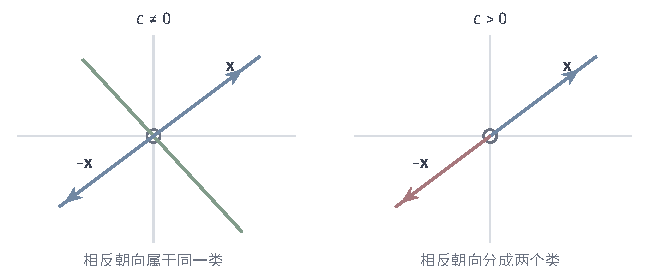
\includegraphics[width=112mm]{figures/01-mathematical-preliminaries-upper/00-shared/tikz/mathematical-language-combinatorics-analysis-optimization-comprehension-additions/equivalence-directions.pdf}
  \caption{平面中非原点的等价分类。每支箭头从原点指向一个点。左侧允许非零实比例，同一直线上的点属于同一类；右侧只允许正比例，同一直线的两侧分成蓝、红两类。绿色表示另一条直线上的类；空心原点不属于被分类的集合。}
  \label{fig:vol1-add-equivalence-directions}
\end{figure}

\subsection{偏序关系}
\label{sec:prelim-order-relations}

\paragraph{偏序与全序}
等价关系把对象分组，另一类常见的关系则用来比较先后或大小。
实数上的$\leq$可以比较任意两个数；集合之间的包含关系却不一定。
在$\mathcal P(\{1,2\})$中，$\varnothing\subseteq\{1\}\subseteq\{1,2\}$，
但$\{1\}$和$\{2\}$互不包含。包含关系可以比较其中一些对象，却不能比较任意两个对象。
下面的定义提炼出这类比较关系共同满足的条件。
\begin{definition}[偏序关系]
\label{def:prelim-partial-order}
集合$X$上的\term{偏序关系}（partial order）$R$是一种允许部分对象互不可比的比较关系：
它对任意$x,y,z\in X$满足反身性$xRx$、传递性（$xRy$且$yRz$蕴含$xRz$），
以及反对称性（$xRy$且$yRx$时必有$x=y$）。
若任意两个元素还至少满足$xRy$或$yRx$中的一个，则称$R$为全序（total order）。
\end{definition}
实数上的$\leq$是全序，因为任意两个实数都可比较。
幂集上的$\subseteq$是偏序：每个集合包含自身，包含关系可以传递，双向包含意味着集合相等；
但它不是全序，因为$\{1\}$与$\{2\}$互不包含。

\paragraph{最小元与最大元}
配备了偏序关系的集合称为偏序集合，记作$(X,\preceq)$，其中$\preceq$表示所选的偏序关系；
实数大小、集合包含等都可作为它的具体解释。
对非空子集$A\subseteq X$，若$a_{\min}\in A$满足$a_{\min}\preceq a$对每个$a\in A$成立，
就称$a_{\min}$为$A$的\term{最小元}（least element）。
若$a_{\max}\in A$满足$a\preceq a_{\max}$对每个$a\in A$成立，
就称$a_{\max}$为$A$的\term{最大元}（greatest element）。
若最小元存在，它必唯一：两个最小元彼此都不大于对方，由反对称性只能相等；最大元同理。

例如在$(\mathcal P(\{1,2\}),\subseteq)$中，整个幂集的最小元是$\varnothing$，最大元是$\{1,2\}$。
但子集族$\{\{1\},\{2\}\}$没有最小元，也没有最大元，因为两者互不可比。

\paragraph{极小元与极大元}
最小元要能与集合中的所有元素比较。若只要求$A$中没有比$a\in A$严格更小的元素，
即$b\in A$且$b\preceq a$必有$b=a$，就称$a$为\term{极小元}（minimal element）。
类似地，若$b\in A$且$a\preceq b$必有$b=a$，就称$a$为\term{极大元}（maximal element）。
最小元一定是极小元，反过来未必成立；最大元与极大元也有相同区别。
在刚才的子集族$\{\{1\},\{2\}\}$中，两个元素都是极小元，也都是极大元，
却都不是最小元或最大元。在全序中任意两元素可比，所以极小元必为最小元，极大元必为最大元。

\paragraph{上界与下界}
最小元和最大元必须属于$A$。若放宽这一要求，允许比较的基准取在$A$以外，就得到界；
不过界仍须属于事先选定的偏序集合$X$。
若$u\in X$满足$a\preceq u$对每个$a\in A$成立，称$u$为$A$的\term{上界}（upper bound）；
若$l\in X$满足$l\preceq a$对每个$a\in A$成立，称$l$为$A$的\term{下界}（lower bound）。
例如对$A=\{\{1\},\{2\}\}\subseteq\mathcal P(\{1,2\})$，
$\varnothing$是下界，$\{1,2\}$是上界，它们都不属于$A$。
因此存在上下界不意味着存在最小元和最大元；反过来，属于$A$的下界就是最小元，属于$A$的上界就是最大元。

\paragraph{上确界与下确界}
若$A$的全部上界组成的集合有最小元，就称它为$A$的上确界，记为$\sup A$；
若全部下界组成的集合有最大元，就称它为$A$的下确界，记为$\inf A$。
在幂集的包含偏序下，子集族的并是上确界，交是下确界：并包含每个成员，因而是上界，
又包含于任何一个共同上界，因而是最小的上界；交的论证方向相反。
于是前例中$\sup A=\{1,2\}$、$\inf A=\varnothing$，但$A$仍无最大元和最小元。
一般偏序集合不保证这些确界存在；第~\ref{sec:prelim-optimal-values-errors}节将在实数中用完备性保证非空有界集合的确界存在。

\section{索引族}
\label{sec:prelim-indices-sums-recurrences}

同一个数可以在一组记录中出现多次。例如记录$(1,1,4)$有三项，取值集合却只有$\{1,4\}$。
本节先用编号保留每次出现，再讨论怎样对这些带编号的对象求和、求积或逐项生成。

\subsection{索引族与序列}
\label{sec:prelim-indexed-sequences}

\paragraph{索引族}
直接把记录组成集合，会丢掉重复值所在的位置。为此给每项记录一个编号，并为每个编号指定唯一的对象。

\begin{definition}[索引族]
\label{def:prelim-indexed-family}
给定索引集合$I$和对象集合$X$，若为每个$i\in I$指定唯一的对象$a_i\in X$，就得到索引族（indexed family）。
整个族写作$(a_i)_{i\in I}$；也可把第$i$项记作$a(i)$。
\end{definition}
开头的记录写成索引族就是$a_1=1,a_2=1,a_3=4$，共有三个编号；
虽然前两个编号对应相同的数，求和时仍应分别计入。
索引集合未必有顺序，例如用城市名索引一组气温时，城市名本身没有规定先后。

\paragraph{序列}
按正整数顺序索引的对象族称为序列（sequence）。
若只取$1,\ldots,n$，就得到有限序列；若取全部正整数，就得到无限序列。
取值为实数的序列称为数列，例如$(1/n)_{n\geq1}$。
序列还可以从$0$开始，此时明写$(a_n)_{n\geq0}$。
带下标的对象族不一定是序列；序列的先后顺序来自整数索引本身的大小顺序。

序列也可以记录逐步更新的结果。若第$t$步的结果还包含多个坐标，就把第$j$个坐标记作$a_j^{(t)}$，其中带括号的上标$t$表示迭代步。
普通上标仍表示幂，所以$a_j^2$与$a_j^{(2)}$不同。

\paragraph{二维索引族}
一项观测含有多个坐标时，需要同时保留观测编号与坐标编号，可以用两个索引共同指定一个对象。
给定索引集合$I,J$及对象集合$X$，为每个$(i,j)\in I\times J$指定唯一对象$a_{i,j}\in X$，就得到二维索引族，
整个族写作$(a_{i,j})_{(i,j)\in I\times J}$。
只有两个索引都确定以后，才指定出一个对象；固定其中一个索引，就得到由另一个索引编号的一族对象。
例如$I=\{1,2\}$、$J=\{1,2,3\}$，令$a_{i,j}=3(i-1)+j$，可排成
\[
 \begin{array}{c@{\quad}ccc}
  &j=1&j=2&j=3\\\hline
 i=1&1&2&3\\
 i=2&4&5&6
 \end{array}.
\]
此时$a_{2,3}=6$；固定$i=2$得到第二行的三项，固定$j=2$得到第二列的两项。
本书在多维索引间写逗号，并在每次使用时说明各索引的范围。

\subsection{集合族的并与交}
\label{sec:prelim-indexed-set-operations}
索引族中的对象也可以是集合。给定索引族$(A_i)_{i\in I}$，其中每个$A_i$都是全集$U$的子集，
两个集合的并与交可以推广到任意多个集合：
\[
 \begin{aligned}
  \bigcup_{i\in I}A_i
  &=\{u\in U:\text{存在 }i\in I\text{ 使 }u\in A_i\},\\
  \bigcap_{i\in I}A_i
  &=\{u\in U:\text{对每个 }i\in I\text{ 都有 }u\in A_i\}.
 \end{aligned}
\]
$I=\{1,2\}$时回到前面的$A_1\cup A_2$与$A_1\cap A_2$；
$I=\{1,2,\ldots\}$时也写成$\bigcup_{n=1}^\infty A_n$。
例如在全集$U=[0,1]$中取$A_n=[1/n,1]$，则$\bigcup_{n\geq1}A_n=(0,1]$：
每个$x\in(0,1]$在$n\geq1/x$时属于$A_n$，而$0$不属于任何$A_n$。

De Morgan律对任意索引族同样成立：
\begin{equation}
 \begin{aligned}
  \left(\bigcup_{i\in I}A_i\right)^{\mathrm c}
  &=\bigcap_{i\in I}A_i^{\mathrm c},\\
  \left(\bigcap_{i\in I}A_i\right)^{\mathrm c}
  &=\bigcup_{i\in I}A_i^{\mathrm c}.
 \end{aligned}
 \label{eq:prelim-de-morgan-families}
\end{equation}
证明与两个集合时相同：$u$不属于并集，等价于对每个$i$都不属于$A_i$；
$u$不属于交集，等价于至少有一个$i$使$u\notin A_i$。
后面测量集合时要对一列无穷多个集合取并与交，用的就是这里的记号和规律。

\subsection{有限和与有限积}
\label{sec:prelim-finite-sums-products}

\paragraph{有限和与有限积}
对$n\geq1$个实数$a_1,\ldots,a_n$，依次相加与相乘分别记为
\[
  \sum_{i=1}^{n}a_i=a_1+\cdots+a_n,\qquad
  \prod_{i=1}^{n}a_i=a_1\cdots a_n.
\]
例如$a_1=1,a_2=4,a_3=9$时，有限和为$14$，有限积为$36$。
若没有任何项，约定
\[
  \sum_{i\in\varnothing}a_i=0,\qquad
  \prod_{i\in\varnothing}a_i=1.
\]
理由是把一组项拆成两部分分别汇总时，若其中一部分为空，结果不应改变：加法需要$0$，乘法需要$1$。
例如从累计值$0$开始逐项相加，尚未加入任何一项时的累计值正好是空和。

\paragraph{哑索引与自由索引}
范围确定后，求和变量的名称不影响结果：
\[
  \sum_{i=1}^{n}a_i=\sum_{k=1}^{n}a_k.
\]
这里$i$是\term{哑索引}（dummy index），它只是“当前加到第几项”的占位记号，
求和完成后不再出现，所以换成任何没在别处用过的字母，结果都不变。

自由索引则不同。设$x_{i,j}$表示第$i$个样本的第$j$个坐标，把$n$个样本的同一坐标加起来，得到
\[
  b_j=\sum_{i=1}^{n}x_{i,j},\qquad j=1,\ldots,d.
\]
其中$j$是自由索引（free index）：固定$j$才能知道在汇总哪个坐标，它也出现在结果$b_j$中。
可以把求和的$i$统一改为$k$，却不能只把右侧的$j$改成$k$而保留左侧的$b_j$。
给哑索引换名时，也不能占用式中已有的自由索引；把本式的$i$改成$j$会破坏原来的含义。

\paragraph{有限和的运算法则}
有限和中的各项可以先乘系数再相加，也可以先分别求和再乘系数。这一规则称为求和的线性关系，
它来自实数加法的交换律、结合律以及乘法对加法的分配律。对实数$a,b$与实数$u_1,\ldots,u_n$、$v_1,\ldots,v_n$，
\[
  \sum_{i=1}^{n}(au_i+bv_i)
  =
  a\sum_{i=1}^{n}u_i+b\sum_{i=1}^{n}v_i.
\]

\paragraph{有限积的运算法则}
有限积可以按对应项相乘后合并，也可以把同一个常数从每一项中提出。对$n\geq1$个实数
$a_i,b_i$和实常数$c$，有
\[
 \prod_{i=1}^n(a_i b_i)
 =\left(\prod_{i=1}^n a_i\right)\left(\prod_{i=1}^n b_i\right),\qquad
 \prod_{i=1}^n(ca_i)=c^n\prod_{i=1}^n a_i.
\]
这些等式来自实数乘法的交换律与结合律；第二式中$c$共出现$n$次。
若每个$b_i\neq0$，还可逐项相除：
\[
 \prod_{i=1}^n\frac{a_i}{b_i}
 =\frac{\prod_{i=1}^n a_i}{\prod_{i=1}^n b_i}.
\]
例如$(2\cdot1)(2\cdot4)(2\cdot9)=2^3(1\cdot4\cdot9)=288$。

有限积没有类似求和的线性关系。取$a_1=1,b_1=2,a_2=3,b_2=4$，则
$\prod_{i=1}^2(a_i+b_i)=(1+2)(3+4)=21$，而$\prod_{i=1}^2a_i+\prod_{i=1}^2b_i=1\cdot3+2\cdot4=11$，
所以一般不能把和的连乘拆成两个连乘之和。

\paragraph{多重求和}
对有限实数数组$(a_{i,j})$，$i=1,\ldots,n$，$j=1,\ldots,d$，可以先按行求和，也可以先按列求和：
\[
  \sum_{i=1}^{n}\sum_{j=1}^{d}a_{i,j}
  =
  \sum_{j=1}^{d}\sum_{i=1}^{n}a_{i,j},
\]
因为两边都遍历$\{1,\ldots,n\}\times\{1,\ldots,d\}$，每个索引对恰好贡献一次；
有限实数加法的交换律和结合律允许改变遍历顺序。
例如数组两行为$(1,2,3)$和$(4,5,6)$，按行汇总得$6+15=21$，
按列汇总得$5+7+9=21$。

如果内层范围依赖外层索引，换序时范围也必须随之重写。例如
\begin{equation}
  \sum_{i=1}^{n}\sum_{j=1}^{i}a_{i,j}
  =
  \sum_{j=1}^{n}\sum_{i=j}^{n}a_{i,j}.
  \label{eq:prelim-triangular-sum}
\end{equation}
两边遍历的索引对都恰好是满足$1\leq j\leq i\leq n$的全部$(i,j)$。$n=3$时共有六项，
分别对应$(1,1)$、$(2,1)$、$(2,2)$、$(3,1)$、$(3,2)$和$(3,3)$。
若把右侧内层误写为$i=1,\ldots,n$，就会遍历全部九个索引对，多算$(1,2)$、$(1,3)$、$(2,3)$三项。
合法换序保留的是同一批项，不只是交换两个求和符号。
无限级数与积分的换序还需要额外条件，不能仅从有限情形类推。

\paragraph{多重求积}
对有限实数数组$(a_{i,j})$，把每个位置的数各乘一次，得到多重积。
由于乘法满足交换律与结合律，矩形索引范围内可以按行或按列求积：
\[
 \prod_{i=1}^n\prod_{j=1}^d a_{i,j}
 =\prod_{j=1}^d\prod_{i=1}^n a_{i,j}.
\]
例如两行为$(1,2,3)$和$(4,5,6)$时，两种次序分别给出
\[
 (1\cdot2\cdot3)(4\cdot5\cdot6)
 =(1\cdot4)(2\cdot5)(3\cdot6)=720.
\]
与多重求和一样，内层范围依赖外层索引时，换序必须保留同一批索引对。例如
\[
 \prod_{i=1}^n\prod_{j=1}^i a_{i,j}
 =\prod_{j=1}^n\prod_{i=j}^n a_{i,j}.
\]
两边都只取满足$1\leq j\leq i\leq n$的位置；这些有限积的换序不要求各项非零。

\subsection{递推关系}
\label{sec:prelim-recurrence-unrolling}

\paragraph{递推关系}
从初值出发、用已经得到的项确定下一项的关系称为\term{递推}（recurrence）。
例如对$a_1=1,a_2=4,a_3=9$，累计和可以写成
\[
 S^{(0)}=0,\qquad S^{(t+1)}=S^{(t)}+a_{t+1},\qquad t=0,1,2.
\]
依次得到$S^{(1)}=1$、$S^{(2)}=5$、$S^{(3)}=14$。
同一组数也可写为$S^{(t)}=\sum_{i=1}^t a_i$：求和式直接给出第$t$项，
递推式则说明如何从前一项得到后一项。初值与更新关系共同确定序列；只有更新关系通常不够。

\paragraph{数学归纳法}
由递推猜出通项公式以后，需要确认公式对\emph{每一个}$t$都成立，而不只对算过的前几项成立。
递推式本身提示了证明方法：若公式在初值处成立，并且“公式对第$t$项成立”总能推出“它对第$t+1$项成立”，
那么从初值出发逐步推进，任何给定的$t$都能在有限步内到达，公式便对全部$t$成立。

这种证明方法称为\term{数学归纳法}（mathematical induction）：要证明关于$t=0,1,2,\ldots$的命题$P(t)$全部成立，
只需证明$P(0)$成立（归纳基础），以及对每个$t\geq0$，由$P(t)$可推出$P(t+1)$（归纳步）。
归纳步中暂时假定的$P(t)$称为归纳假设。

以前面的累计和为例，命题$P(t)$为$S^{(t)}=\sum_{i=1}^ta_i$。
$P(0)$成立，因为$S^{(0)}=0$恰是空和。若$P(t)$成立，则
$S^{(t+1)}=S^{(t)}+a_{t+1}=\sum_{i=1}^ta_i+a_{t+1}=\sum_{i=1}^{t+1}a_i$，即$P(t+1)$成立。
所以递推式与求和式对每个$t$描述同一个序列。

\paragraph{等差递推}
若每一步都增加同一个实数$d$，就得到等差递推：
\[
 a^{(t+1)}=a^{(t)}+d,\qquad a^{(0)}=a_0,\qquad t=0,1,\ldots.
\]
从初值到第$t$步共加了$t$次$d$，因此
\[
 a^{(t)}=a_0+td.
\]
用归纳法写出来：$t=0$时右侧为$a_0$；若$a^{(t)}=a_0+td$，则$a^{(t+1)}=a_0+td+d=a_0+(t+1)d$。
例如从$2$开始，每步加$3$，依次得到$2,5,8,11,\ldots$，第$t$步为$2+3t$。
$d>0$时各项递增，$d<0$时各项递减，$d=0$时保持初值。

\paragraph{等比递推}
从$8$开始，每一步乘$1/2$，便依次得到$8,4,2,1,\ldots$。
用$e^{(t)}$表示第$t$项，把$1/2$推广为固定系数$\rho\in\mathbb{R}$，可写成
\begin{equation}
  e^{(t+1)}=\rho e^{(t)},\qquad e^{(0)}=e_0,\qquad t=0,1,\ldots,
  \label{eq:prelim-geometric-recurrence}
\end{equation}
逐步展开得到
\[
  e^{(t)}=\rho^t e_0,\qquad t=0,1,2,\ldots
\]
（约定$\rho^0=1$）。归纳步只需一行：若$e^{(t)}=\rho^te_0$，则$e^{(t+1)}=\rho\cdot\rho^te_0=\rho^{t+1}e_0$。
每步都有$|e^{(t+1)}|=|\rho|\,|e^{(t)}|$：当$|\rho|<1$时，非零项的绝对值在下一步缩小；
$\rho=-1$使大小不变而符号交替，$|\rho|>1$使非零项的绝对值放大。
若$e_0=0$，每一项都是零；若$\rho=0$，第一次更新后便一直为零。

\paragraph{有限几何和}
等比序列的各项相加，得到有限几何和$G_N=\sum_{n=0}^N\rho^n=1+\rho+\cdots+\rho^N$。
它可以用“错位相减”求出：把$G_N$乘以$\rho$，每一项都向后移一位，
\[
 \rho G_N=\rho+\rho^2+\cdots+\rho^{N+1}.
\]
两式相减时，中间各项成对抵消，只剩首项$1$与末项$\rho^{N+1}$：$(1-\rho)G_N=1-\rho^{N+1}$。因此
\begin{equation}
 \sum_{n=0}^N\rho^n=\frac{1-\rho^{N+1}}{1-\rho}\qquad(\rho\neq1),
 \qquad\sum_{n=0}^N1^n=N+1.
 \label{eq:prelim-finite-geometric-sum}
\end{equation}
例如$\rho=1/2$、$N=3$时，$1+1/2+1/4+1/8=15/8$，与$(1-1/16)/(1/2)$相同。
这种“相邻项抵消”的做法也适用于一般的差：对任意数列$(b_n)$，
\begin{equation}
 \sum_{n=1}^N(b_{n+1}-b_n)=b_{N+1}-b_1,
 \label{eq:prelim-telescoping-sum}
\end{equation}
因为展开后每个中间的$b_n$恰好以正、负号各出现一次。这称为裂项求和。
例如$\frac1{n(n+1)}=\frac1n-\frac1{n+1}$，所以$\sum_{n=1}^N\frac1{n(n+1)}=1-\frac1{N+1}$。
这里先由更新规则确定有限步结果；$N$无限增大时这些和怎样变化，将在第~\ref{chap:function-limits}章讨论。

\section{函数与函数族}
\label{sec:prelim-functions-value-ranges}

索引族记录的是已经得到的数值；预测还需要一条由输入算出输出的规则。
二元关系允许一个输入关联多个输出，也允许某些输入没有输出；
用规则预测时，我们需要更确定的对应：每个允许的输入都恰好给出一个输出。
平方运算把每个实数$x$对应到$x^2$，就是这样的对应。

本节先把这种对应定义为函数，区分预先规定的输出范围与实际取得的输出；
随后说明怎样组合函数、什么时候可以由输出反求输入；
再把函数本身作为集合的元素，研究由参数编号的函数族；
最后比较实值函数的取值大小，引入界、确界和最值。

\subsection{函数的定义}
\label{sec:prelim-function-definition}

\paragraph{函数}
设$X,Y$是两个集合。若$X$到$Y$的关系使每个$x\in X$\emph{恰好}与一个$y\in Y$有关系，
就把这个对应称为\term{函数}（function），也称映射（mapping），记作$f:X\to Y$，
并把与$x$对应的唯一元素记为$f(x)$。
$X$称为定义域（domain），$Y$称为陪域（codomain），$f(x)$称为$f$在$x$处的函数值。
记号$x\mapsto f(x)$表示“把$x$对应到$f(x)$”。

用关系的语言说，函数就是满足“每个$x$恰有一个$y$使$(x,y)\in R$”的关系$R\subseteq X\times Y$；
这个关系本身，即集合$\{(x,f(x)):x\in X\}$，称为函数的图像（graph）。
例如$f:\mathbb R\to\mathbb R$、$f(x)=x^2$在$x=-2$处的函数值为$4$；
“不大于”关系却不是函数，因为同一个$x$与无限多个$y$有关系。

声明一个函数需要同时说明定义域、陪域和对应规则；只写一个表达式，还没有完全规定函数。
两个函数相等，要求这三项分别相同。例如$x\mapsto x^2$作为$\mathbb R\to\mathbb R$与作为$[0,\infty)\to\mathbb R$，
是两个不同的函数；后面判断能否由输出反求输入时，这一区别会改变结论。

从$X$到$Y$的全部函数组成的集合记为$Y^X$。当$X=\{1,\ldots,n\}$、$Y=\mathbb R$时，
一个函数$f$就是$n$个按编号排好的实数$f(1),\ldots,f(n)$，第~\ref{chap:linear-operations}章把这样一列数记作$n$维坐标向量；
前面的索引族$(a_i)_{i\in I}$也正是从$I$到$X$的函数$i\mapsto a_i$。

\paragraph{像与值域}
对定义域中的子集$A\subseteq X$，所有实际得到的输出组成集合
\[
 f(A)=\{f(x):x\in A\},
\]
称为$A$在$f$下的像（image）。整个定义域的像$f(X)$称为函数的值域。
陪域是预先规定的输出范围，值域是实际取得的全部输出，因而$f(X)\subseteq Y$。
对平方函数，$f(\{-2,1\})=\{1,4\}$，值域是$[0,\infty)$，真包含于陪域$\mathbb R$。

\paragraph{原像}
给定输出的一个范围$B\subseteq Y$，可以反过来收集所有使输出落在$B$中的输入：
\begin{equation}
 f^{-1}(B)=\{x\in X:f(x)\in B\}.
 \label{eq:prelim-preimage}
\end{equation}
这称为$B$在$f$下的\term{原像}（preimage）。原像是定义域的子集。
对平方函数，逐项解相应条件得到
\[
 \begin{aligned}
 f^{-1}(\{1\})&=\{-1,1\},\\
 f^{-1}([1,4])&=[-2,-1]\cup[1,2],\\
 f^{-1}(\{-1\})&=\varnothing.
 \end{aligned}
\]
因此原像可以包含多个元素，也可以为空。
记号$f^{-1}(B)$作用在集合$B$上，结果也是集合；它本身不要求$f$存在逆映射（逆映射见第~\ref{sec:prelim-function-types}节）。

原像与集合运算相容：对$B,B'\subseteq Y$，
\[
 \begin{aligned}
  f^{-1}(B\cup B')&=f^{-1}(B)\cup f^{-1}(B'),\\
  f^{-1}(B\cap B')&=f^{-1}(B)\cap f^{-1}(B'),\\
  f^{-1}(Y\setminus B)&=X\setminus f^{-1}(B).
 \end{aligned}
\]
以第三式为例，$x\in f^{-1}(Y\setminus B)$当且仅当$f(x)\notin B$，也就是$x\notin f^{-1}(B)$；
前两式同样只需把“$f(x)$属于并集或交集”逐字改写。

像则没有完全相同的性质。像保持并，即$f(A\cup A')=f(A)\cup f(A')$，但一般不保持交：
对平方函数，$f(\{-1\}\cap\{1\})=f(\varnothing)=\varnothing$，而$f(\{-1\})\cap f(\{1\})=\{1\}$。
原像保持补集、并与交，这一性质将在后文判断哪些函数“可测”时反复使用。

\subsection{函数的运算}
\label{sec:prelim-map-operations}

已有的函数可以组合成新的函数。函数值是实数时，可以在每个输入处对函数值做四则运算；
更一般地，可以把一个函数的输出作为另一个函数的输入。

\paragraph{实值函数的四则运算}
若$f,g:X\to\mathbb R$有相同定义域，可以在每个输入处计算函数值的和、差、积：
\[
 \begin{aligned}
 (f+g)(x)&=f(x)+g(x),\\
 (f-g)(x)&=f(x)-g(x),\\
 (fg)(x)&=f(x)g(x).
 \end{aligned}
\]
对实常数$c$，定义
\[
  (cf)(x)=cf(x).
\]
这些新函数的定义域仍是$X$。

商函数则只在分母不为零的范围内定义：
\[
  (f/g)(x)=f(x)/g(x),
\]
其定义域为$\{x\in X:g(x)\neq0\}$。例如在$\mathbb R$上取$f(x)=x$、$g(x)=x-1$，则$(f+g)(x)=2x-1$定义在整个实轴上，
而$(f/g)(x)=x/(x-1)$的定义域不含$1$。

\paragraph{函数的复合}
若$f:X\to Y$、$g:Y\to Z$，先用$f$求值，再把结果送入$g$，就得到\term{复合}函数
（composition）$g\circ f:X\to Z$，定义为
\[
 (g\circ f)(x)=g(f(x)).
\]
例如$f(x)=x^2$、$g(x)=x+1$时，
$(g\circ f)(x)=x^2+1$，而$(f\circ g)(x)=(x+1)^2$。
在$x=1$处，两者分别为$2$和$4$，所以复合的次序一般不能交换。

复合有意义的前提是前一个函数的每个输出都属于后一个函数的定义域，即$f(X)$包含于$g$的定义域。
若条件不满足，就要先缩小前一个函数的定义域。
例如$f:\mathbb R\to\mathbb R$、$f(x)=x-1$与$g:[0,\infty)\to\mathbb R$、$g(u)=\sqrt u$不能直接复合，
因为$f$有负的输出；只有把$f$限制在使$f(x)\geq0$的输入$x\geq1$上，才能定义$(g\circ f)(x)=\sqrt{x-1}$。

复合的次序一般不能交换，括号的位置却可以改变。对$f:X\to Y$、$g:Y\to Z$、$h:Z\to W$，
按定义逐层代入，$(h\circ(g\circ f))(x)=h((g\circ f)(x))=h(g(f(x)))$，
而$((h\circ g)\circ f)(x)=(h\circ g)(f(x))=h(g(f(x)))$。
两种括号方式在每个$x$处给出相同的值，定义域与陪域也相同，故
\[
 h\circ(g\circ f)=(h\circ g)\circ f.
\]
这称为复合的结合律，因此多次复合可以不写括号，记作$h\circ g\circ f$。

\subsection{函数的类型}
\label{sec:prelim-function-types}

原像回答“哪些输入给出这些输出”，答案是一个集合。若希望由陪域中的每个输出\emph{唯一地}恢复输入，
就要求函数既不把两个不同输入送到同一个输出，又不遗漏陪域中的任何元素。
下面先引入“什么都不改变”的恒等映射，作为描述“撤销”的基准；再把上述两项要求分别定义为单射与满射，
最后说明二者同时成立时怎样定义逆映射。

\paragraph{恒等映射}
把每个元素送回自身的映射$\operatorname{id}_X:X\to X$，
$\operatorname{id}_X(x)=x$，称为恒等映射（identity map）。
对$f:X\to Y$，有$f\circ\operatorname{id}_X=f$、$\operatorname{id}_Y\circ f=f$：
恒等映射在复合中不改变原函数，作用类似于数$1$在实数乘法中的作用。

\paragraph{单射}
若不同输入的输出总不相同，就称$f:X\to Y$为\term{单射}（injection）。
等价地，$f(x_1)=f(x_2)$必定推出$x_1=x_2$。
平方函数$f:\mathbb R\to\mathbb R$不是单射，因为$f(-1)=f(1)$；
把定义域限制为$[0,\infty)$后，它就成为单射。

\paragraph{满射}
若陪域中的每个元素都能由某个输入取得，即$f(X)=Y$，就称$f$为\term{满射}（surjection）。
平方函数$\mathbb R\to\mathbb R$不是满射，因为负数取不到；
把陪域改为$[0,\infty)$后，它就是满射。
单射要求不同输入的输出互不相同，满射要求实际输出覆盖整个陪域，两项要求互不包含。

\paragraph{双射与逆映射}
\phantomsection
\label{def:prelim-invertible-map}
同时为单射和满射的函数$f:X\to Y$称为双射（bijection）。
对双射，满射保证每个$y\in Y$至少有一个原输入，单射保证至多有一个，所以恰有一个原输入$x\in X$。
把$y$对应到这个$x$的函数称为逆映射（inverse map），记作$f^{-1}:Y\to X$，满足
\[
 f^{-1}\circ f=\operatorname{id}_X,\qquad
 f\circ f^{-1}=\operatorname{id}_Y.
\]
例如$g:[0,\infty)\to[0,\infty)$、$g(x)=x^2$是双射，
其逆映射为$g^{-1}(y)=\sqrt y$。若定义域取整个$\mathbb R$，就无法从平方值唯一恢复原输入。

反过来，若存在$h:Y\to X$使$h\circ f=\operatorname{id}_X$且$f\circ h=\operatorname{id}_Y$，则$f$必为双射：
对$f(x_1)=f(x_2)$两边作用$h$得$x_1=x_2$，所以$f$是单射；每个$y$都等于$f(h(y))$，所以$f$是满射。
因此“可以双向撤销”与“双射”是同一个条件。
从一元函数的图像看，单射意味着每条水平线至多与图像相交一次；
满射意味着陪域中的每个高度，图像上都至少有一个点。

图~\ref{fig:prelim-preimage-inverse}用有限集合说明两种反向操作。
沿指向$1$的全部箭头寻找原像，可以得到两个输入；
逆映射则要求每个输出有且只有一个箭头来源。

\begin{figure}[htbp]
  \centering
  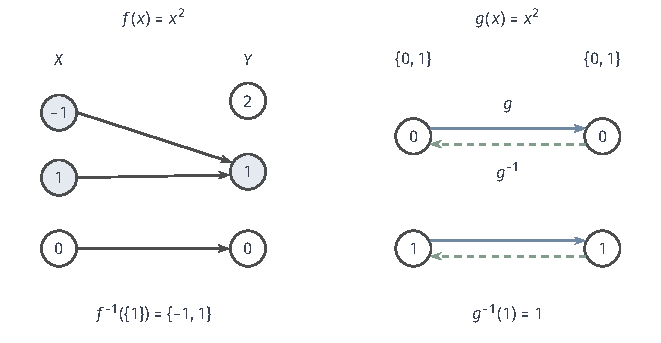
\includegraphics[width=112.0mm]{figures/01-mathematical-preliminaries-upper/01-mathematical-language-combinatorics-analysis-optimization/tikz/prelim-preimage-inverse/figure.pdf}
  \caption{原像与逆映射回答不同问题。左侧$f:\{-1,0,1\}\to\{0,1,2\}$按平方取值，
  标出的$1$有两个原输入，$2$没有原输入；原像$f^{-1}(\{1\})=\{-1,1\}$仍有定义。
  右侧将定义域与陪域都限制为$\{0,1\}$得到双射$g$，实线表示正向求值，虚线表示
  逆映射，因而$g^{-1}(1)=1$是一个元素。两侧均为精确的有限映射。}
  \label{fig:prelim-preimage-inverse}
\end{figure}

双射复合后的反求需要倒转次序。若$f:X\to Y$与$g:Y\to Z$都是双射，
先撤销$g$，再撤销$f$，有
\begin{equation}
 (g\circ f)^{-1}=f^{-1}\circ g^{-1}.
 \label{eq:prelim-inverse-composition}
\end{equation}
验证时分别代入$x\in X$与$z\in Z$：
\[
 \begin{aligned}
 f^{-1}(g^{-1}(g(f(x))))&=x,\\
 g(f(f^{-1}(g^{-1}(z))))&=z.
 \end{aligned}
\]
例如取双射$f:[0,\infty)\to[0,\infty)$、$f(x)=x^2$与$g:[0,\infty)\to[1,\infty)$、$g(u)=u+1$，
复合$g\circ f$先平方、再加$1$，把非负数$x$变成$z=x^2+1$。
反求时次序倒转：先减$1$、再开平方，得到$x=\sqrt{z-1}$，其定义域为$[1,\infty)$。

\subsection{函数族与参数化}
\label{sec:prelim-function-families}

\paragraph{函数族}
回到本章开头的预测问题。我们事先并不知道哪条规则最合适，通常先划定一批候选规则，再从中挑选。
这批候选规则本身是一个集合，它的元素是整个函数。
具有同一定义域和陪域的一组函数组成函数族（family of functions）。

例如，形如$f(x)=ax+b$的函数称为一元仿射函数（affine function），所有这样的函数组成
\[
 \mathcal F=\{f_{a,b}:\mathbb R\to\mathbb R:\ f_{a,b}(x)=ax+b,\ (a,b)\in\mathbb R^2\}.
\]
族中的每个元素是一整个函数。取$(a,b)=(2,1)$得到函数$f_{2,1}(x)=2x+1$；
再取输入$x=3$，才得到一个函数值$f_{2,1}(3)=7$。

\paragraph{函数参数化}
用参数为函数族中的函数编号，称为参数化（parameterization）。
一般写成$\theta\mapsto f_\theta$，其中$\theta$属于参数集合$\Theta$，
$f_\theta:X\to Y$是相应的函数。
映射$\theta\mapsto f_\theta$的输入是参数，输出是函数；函数$f_\theta$自身的输入仍是$x$。
在上例中，$\theta=(a,b)$指定一条直线，而$x$指定在直线上的哪个位置求值。
参数化把“在函数中挑选”改写为“在参数集合中挑选”；参数集合通常是$\mathbb R^2$这样熟悉的集合，
便于后续用数值方法比较和调整。

\paragraph{函数参数化的可识别性}
不同参数可能表示同一个函数，所以参数与函数未必一一对应。能否由函数反过来确定参数，取决于下面的条件。
\begin{definition}[函数参数化的可识别性]
\label{def:prelim-identifiable-parameterization}
给定参数集合$\Theta$与函数族$\{f_\theta:X\to Y:\theta\in\Theta\}$。
若$f_\theta=f_{\theta'}$蕴含$\theta=\theta'$，即$\theta\mapsto f_\theta$为单射，
则称这一函数参数化可识别（identifiable）；也就是说，完整函数唯一确定其参数。
否则称为不可识别。
\end{definition}
这里比较的是整个定义域上的函数，而非几个位置的函数值。
例如仿射函数族中$b=f_{a,b}(0)$、$a=f_{a,b}(1)-f_{a,b}(0)$，
所以完整函数唯一确定$(a,b)$，这一参数化可识别。若只观察$x=0$处的函数值，则只能确定$b$，
不能确定$a$。可见，有限个观测是否足以确定参数，与参数化是否可识别是两个不同的问题。

\Needspace{11\baselineskip}
\begin{example}[参数不同而函数相同]
\label{ex:prelim-nonidentifiable-parameterization}
考虑参数化函数
\[
  f_{a,b}:\mathbb{R}\to\mathbb{R},
  \qquad
  f_{a,b}(x)=abx,
  \qquad
  (a,b)\in\mathbb{R}^2.
\]
参数$(1,2)$与$(2,1)$不同，却对每个$x$给出相同的函数值。更一般地，只要$c\neq0$，
$(ca,b/c)$与$(a,b)$就表示同一个函数。从完整的输入输出关系可以确定乘积$ab$（例如取$x=1$，有$ab=f_{a,b}(1)$），
却不能分别确定$a$和$b$。这是参数化本身不可识别，而不是计算精度不足。
\end{example}


图~\ref{fig:vol1-add-parameter-function-value}把“由参数得到函数”和“由函数得到函数值”这两层操作分开：三组不同参数先汇入同一条完整规则，然后才在指定的$x$处求值。
\begin{figure}[!htb]
  \centering
  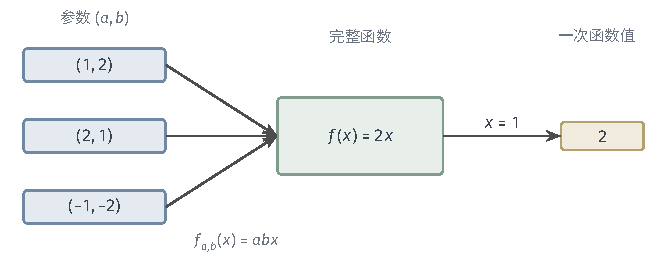
\includegraphics[width=112mm]{figures/01-mathematical-preliminaries-upper/00-shared/tikz/mathematical-language-combinatorics-analysis-optimization-comprehension-additions/parameter-function-value.pdf}
  \caption{参数化$f_{a,b}(x)=abx$中的三层对象。参数$(1,2),(2,1),(-1,-2)$的乘积均为$2$，所以它们表示同一个函数$f(x)=2x$；再指定$x=1$，才得到一次求值结果$2$。多组参数汇入同一完整函数，正是不可识别性。}
  \label{fig:vol1-add-parameter-function-value}
\end{figure}

不可识别的参数可以用前面的等价关系整理。规定$\theta\sim\theta'$当且仅当$f_\theta=f_{\theta'}$，
就得到参数集合上的等价关系：函数相等本身是反身、对称、传递的，三条性质直接继承。
每个等价类收集同一个函数的全部参数表示；在$f_{a,b}(x)=abx$中，$(a,b)$所在的等价类是满足$a'b'=ab$的全部参数$(a',b')$。

把每个等价类对应到它所表示的函数，就得到从商集$\Theta/{\sim}$到函数族$\{f_\theta:\theta\in\Theta\}$的双射。
参数化可识别，恰好意味着每个等价类只含一个参数。
换言之，函数族中的元素按函数区分，参数则可能为同一个函数保留多种表示。

\subsection{实值函数的界与极值}
\label{sec:prelim-optimal-values-errors}

从候选函数中挑选时，常把每个候选的优劣写成一个实数，例如预测误差，再寻找使它最小的候选。
这就要求讨论一个实值函数能取到多小的值、最小值是否真的取得。
函数值组成实数集合，而实数的通常大小$\leq$是全序。下面先把偏序集合中的界与确界用于实数，
说明保证确界存在的实数完备性，再把这些概念用于函数。

\paragraph{上界与下界}
设$A\subseteq\mathbb R$非空。若$a\leq M$对每个$a\in A$成立，
就称$M$为$A$的上界（upper bound）；若$m\leq a$对每个$a\in A$成立，
就称$m$为下界（lower bound）。这正是前面偏序集合中上界、下界的定义在$(\mathbb R,\leq)$中的情形。
存在上界称为上有界，存在下界称为下有界，两者都有称为有界。
例如$(0,1)$有上界$1,2$，也有下界$0,-1$。界不必是集合中的元素，也不唯一。

\paragraph{上确界与下确界}
上界中的最小者称为\term{上确界}（supremum），记作$\sup A$；
下界中的最大者称为\term{下确界}（infimum），记作$\inf A$。
例如$\sup(0,1)=1$、$\inf(0,1)=0$，两个确界都不属于$(0,1)$。

上确界$\beta$不仅要满足$a\leq\beta$对所有$a\in A$成立，
还要满足每个$\varepsilon>0$都存在$a\in A$使$a>\beta-\varepsilon$。
后一个条件说明，任何比$\beta$小的数都不是上界。
下确界$\alpha$类似地满足$\alpha\leq a$对所有$a\in A$成立，且每个$\varepsilon>0$都存在$a\in A$
使$a<\alpha+\varepsilon$。

上界有无限多个，其中是否真有最小的一个，并不能从定义直接看出。
本书把下面的性质作为实数的基本性质使用，称为实数的完备性（也称确界原理）：
非空上有界实数集合有实数上确界，非空下有界实数集合有实数下确界。
有理数没有这一性质：集合$\{q\in\mathbb Q:q^2<2\}$在有理数中有上界（例如$2$），
但它在实数中的上确界是$\sqrt2$，而$\sqrt2$不是有理数。于是每个有理上界都严格大于$\sqrt2$，
在它与$\sqrt2$之间总还有更小的有理上界，所以在有理数中找不到最小的上界。
实数补上了这样的“空隙”，后面关于极限存在的结论都要用到这一点。

\paragraph{函数的有界性}
对非空定义域$X$上的实值函数$f:X\to\mathbb R$，讨论其有界性就是讨论值域$f(X)$的有界性。
例如$f(x)=x$在$(0,1)$上有界，在$\mathbb R$上则既无上界也无下界。
值域的确界简记为
\[
 \inf_{x\in X}f(x)=\inf f(X),\qquad
 \sup_{x\in X}f(x)=\sup f(X).
\]
若$f(X)$无下界，约定其下确界为$-\infty$；若无上界，约定其上确界为$+\infty$。
这两个符号表示没有有限的界，不是实值函数实际取到的数。

\paragraph{最小值与最小点}
若存在$x^\star\in X$使
\[
 \forall x\in X,\qquad f(x^\star)\leq f(x),
\]
则称$x^\star$为\term{全局最小点}（global minimizer），$f(x^\star)$为最小值。
符号$\forall$读作“对所有”，这里要求与定义域内的每个函数值比较。
最小值记作$\min_{x\in X}f(x)$；全部最小点组成的集合记作
\[
 \argmin_{x\in X}f(x)
 =\{x\in X:\ f(x)\leq f(z)\text{ 对所有 }z\in X\}.
\]
$\min$给出一个数，$\argmin$给出输入的集合；若不存在最小点，后一个集合为空。

最小值存在时必等于下确界：$f(x^\star)$不超过每个函数值，所以是值域的一个下界；
任何下界$m$都满足$m\leq f(x^\star)$，因为$f(x^\star)$本身就是一个函数值。
所以$f(x^\star)$是最大的下界。反过来，下确界存在却未必被取得。
例如$f(x)=x$在$(0,1)$上的下确界为$0$，但没有最小点，
因为任意允许的$x$都有更小的允许输入$x/2$。

\paragraph{最大值与最大点}
若存在$x^\star\in X$使$f(x^\star)\geq f(x)$对所有$x\in X$成立，
则称$x^\star$为全局最大点，$f(x^\star)$为最大值。
最大值记作$\max_{x\in X}f(x)$，全部最大点组成
\[
 \argmax_{x\in X}f(x)
 =\{x\in X:\ f(x)\geq f(z)\text{ 对所有 }z\in X\}.
\]
与最小值的论证对称，最大值存在时等于上确界。函数$f(x)=x$在$(0,1)$上没有最大值；
将定义域换为$[0,1]$后，最大值为$1$、最大点为$1$，最小值为$0$、最小点为$0$。

\begin{example}[同一个最优值可以对应多个输入]
\label{ex:prelim-optimal-value-versus-points}
令$X=[-2,2]$，$f(x)=(x^2-1)^2$。平方非负，且$x=\pm1$都使它为零，所以
\[
  \min_{x\in X}f(x)=\inf_{x\in X}f(x)=0,\qquad
  \argmin_{x\in X}f(x)=\{-1,1\}.
\]
又因为$0\leq x^2\leq4$，有$|x^2-1|\leq3$，于是$f(x)\leq9$，等号恰在$x=\pm2$
处成立。因此最大值为$9$，最大点集合为$\{-2,2\}$。最小值是一个数，不会因为有两个
最小点就变成两个最小值；最优点是否唯一是另一个问题。
\end{example}

图~\ref{fig:prelim-minimum-infimum}固定表达式$f(x)=x$，比较它在$(0,1)$与$[0,1]$上定义的两个函数。
两侧的函数值都以$0$为下确界；右侧把$x=0$纳入定义域后，这个下确界才由某个输入取得。
区别的关键在于边界点是否属于定义域，而不在于两条曲线是否趋向同一个高度。

\begin{figure}[htbp]
  \centering
  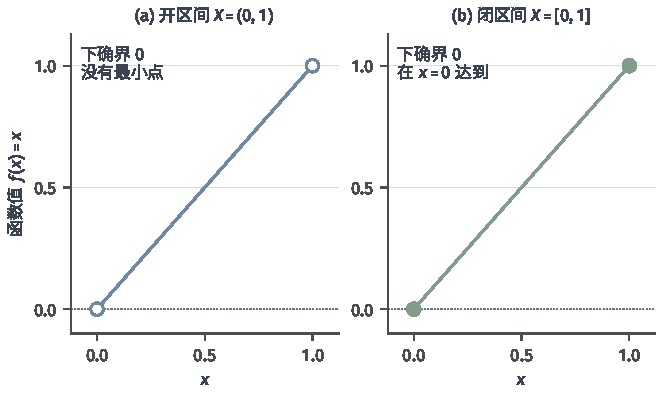
\includegraphics[width=112.0mm]{figures/01-mathematical-preliminaries-upper/01-mathematical-language-combinatorics-analysis-optimization/matplotlib/prelim-minimum-infimum/figure.pdf}
  \caption{同一求值表达式$f(x)=x$在两个定义域上的边界对照。左图定义域为$(0,1)$，空心端点不属于图像，函数值可任意接近$0$，却不能取到；右图定义域为$[0,1]$，实心端点$(0,0)$达到下确界。两图的下确界相同，最小点是否存在取决于可行端点是否保留。图为解析教学示例。}
  \label{fig:prelim-minimum-infimum}
\end{figure}
\FloatBarrier

\section{本章小结}
\label{sec:prelim-sets-functions-summary}

回到开头的四个问题：允许的输入和输出由集合规定，输入到输出的对应由函数描述，
候选规则由函数族与参数化编号、由界与最值比较，多次观测的数值则由索引族编号、由有限和与有限积汇总。

集合的运算满足交换、结合、分配与De Morgan律，两个集合相等可以拆成双向包含来证明。
二元关系把满足条件的有序对收集为笛卡尔积的子集；
关系的自反、对称与传递闭包分别补入对应性质所必需的有序对。
等价关系恰好对应集合的划分，偏序关系允许部分对象互不可比；最小元与极小元、界与集合内的最值需要分别判断。
索引族保留各项的编号与重复出现，集合族的并与交把两个集合的运算推广到任意多个。
有限和、有限积和递推描述这些项怎样汇总或生成，数学归纳法确认由递推得到的通项对每一步都成立，
有限几何和与裂项求和则是后文估计无限求和的起点。

函数是每个输入恰有一个输出的关系：像与原像分别沿输出和输入方向收集对象，原像保持并、交与补，
逆映射则要求函数为双射，也就是可以双向撤销；复合满足结合律，但一般不能交换次序。
函数族以整个函数为元素，参数化为这些函数编号，不同编号可以对应同一个函数。
比较候选函数时，确界原理保证非空定义域上有界函数的值域有上、下确界，但最值是否取得还要另外判断。

这些对象与记号是后续讨论的共同起点：第~\ref{chap:combinatorics}章研究集合的有限计数与基数比较，
第~\ref{chap:function-limits}章研究极限；第~\ref{chap:linear-operations}章起的线性空间部分把有限组数值排成向量与矩阵，
并在其上建立线性运算；随后第~\ref{chap:univariate-differentiation}章、第~\ref{chap:univariate-integration}章和第~\ref{chap:multivariate-calculus}章分别研究一元函数的微分、一元函数的积分与多元微积分。

\chapter{集合的计数}
\label{chap:combinatorics}

有限集合的大小是元素个数。例如四门课中任取一些课程，每一种选择对应一个子集，
计数就是求这样的子集有多少个。答案看似只需逐个列举，但对象稍多时列举既费力又容易重复或遗漏；
我们需要能从问题结构直接算出数量的规则。另一方面，后文比较候选函数时，函数类往往含有无限多个函数，
直接计数没有意义；不过在固定的几个输入上，许多函数会给出相同的输出，这时可以改数不同的输出模式。

本章先建立有限集合的计数方法，再把同样的思路用于函数在有限输入上的输出模式。
前置内容是第~\ref{chap:sets-functions-and-proofs}章的集合运算、函数（特别是双射）、有限求和与数学归纳法。
区间长度与更一般集合的测量将在下一章介绍，因为可数覆盖的构造还需要数列和级数的收敛知识。

\section{有限集合的计数}
\label{sec:comb-families-counting}

计数前必须确定什么算一个结果。从四个对象中依次取两个，$(1,3)$与$(3,1)$是不同的有序记录；
只保留选中的对象时，它们都表示子集$\{1,3\}$。同一批选择采用不同的记录方式，数量就不同。
本节先用双射比较两个集合的大小，再由加法规则、乘法规则推出排列数与组合数，
用它们计数子集与划分，最后处理类别重叠时的校正，以及由子集累计值恢复单个贡献的反演。
以下令$V=\{1,\ldots,n\}$为有限集合，$n\geq0$；数值例子使用$V_0=\{1,2,3,4\}$。

\subsection{基础计数方法}
\label{sec:comb-decomposition-counting}
\label{sec:comb-finite-counting}
\label{sec:comb-classification-products}

全部计数方法都基于三件事：把要数的集合换成一个更容易数的集合；把它分成互不重叠的几类；
或把每个结果拆成依次进行的几步选择。下面先说明这三条规则，再用它们推出排列和组合的公式。

\subsubsection{加法规则和乘法规则}
\label{sec:comb-classification-counting}

\paragraph{双射与计数}
有限集合$A$的元素个数记为$|A|$。“数出$A$有$n$个元素”的含义，就是把元素依次编号为$1,\ldots,n$，
也就是给出一个双射$\{1,\ldots,n\}\to A$。由此得到最基本的计数原则：
若两个有限集合之间存在双射，则它们的元素个数相同。
理由是双射与编号复合仍是双射：若$g:\{1,\ldots,n\}\to A$是编号、$f:A\to B$是双射，则$f\circ g$就是$B$的编号。
这条原则允许我们把难数的集合换成好数的集合，只要找到两者之间的一一对应。
后面计数子集时，就是先把子集一一对应到零一记录。

\paragraph{加法规则}
一项选择若分为互不重叠的几类，可以分别数出各类，再把数量相加。
用集合表示，若有限集合$A_1,\ldots,A_r$两两不交，则
\[
 \left|\bigcup_{i=1}^r A_i\right|=\sum_{i=1}^r|A_i|.
\]
这称为计数的加法规则。它来自编号的拼接：先给$A_1$的元素编号$1,\ldots,|A_1|$，
再接着给$A_2$的元素编号，依此类推；两两不交保证没有元素被编号两次，
各类的并等于全部结果保证没有元素被遗漏，所以最后的编号恰好到$\sum_i|A_i|$。
例如从两本数学书和三本计算机书中选一本，若这两类没有共同的书，共有$2+3=5$种选择。
若同一本书同时列在两类中，就不能直接相加；重叠情形将在容斥原理中处理。

\paragraph{乘法规则}
\phantomsection
\label{sec:comb-stepwise-counting}
一次结果若由若干个位置上的选择组成，并且各位置的任意选择都可组合成结果，就可以用乘法计数。
对有限集合$A_1,\ldots,A_r$，笛卡尔积中的每个结果是一个有序记录，故
\[
 |A_1\times\cdots\times A_r|=\prod_{i=1}^r|A_i|.
\]
这称为计数的乘法规则。$r=2$时，按第一个位置的取值把$A_1\times A_2$分成$|A_1|$类，
第$a$类是$\{a\}\times A_2$，它与$A_2$之间有双射$(a,b)\mapsto b$，所以每类有$|A_2|$个元素；
加法规则给出总数$|A_1|\cdot|A_2|$。一般的$r$再对位置个数用数学归纳法：
$A_1\times\cdots\times A_{r+1}$与$(A_1\times\cdots\times A_r)\times A_{r+1}$之间有显然的双射。
例如第一位取$a,b$之一，第二位取$1,2,3$之一，
共有$2\times3=6$个结果：$(a,1),(a,2),(a,3),(b,1),(b,2),(b,3)$。
长度为$n$的零一记录是$\{0,1\}^n$中的元素，每位有两个选项，因此共有$2^n$条。

分步选择时，后一步的可选对象常依赖前一步的结果，例如先选组长、再从其余人中选记录员。
这时各步的选项集合不同，但只要第$i$步在每种已有记录后都恰有$n_i$个可选结果，
完整记录数仍是$\prod_i n_i$：按第一步的结果分类，每类内部的完整记录数相同，
加法规则把这些相同的数相加，就得到第一步的选项数乘以每类的数量，再对步数归纳。
关键在于选项\emph{个数}不随前面的选择改变，而选项的具体内容可以改变。

\paragraph{等倍归并}
有时直接数出的记录比真正关心的结果多，而每个结果恰好被记录了相同的次数。
设记录的集合$A$按所表示的结果分成若干类，每类恰有$k$个记录，那么结果的个数是$|A|/k$：
加法规则给出$|A|=k\times(\text{结果个数})$。
这一规则要求每个结果被记录的次数\emph{相同}；若次数不同，就不能统一相除。
后面由排列推出组合、由有名称的划分推出无名称的划分，用的都是这条规则。

\subsubsection{排列数和组合数}
\label{sec:comb-permutation-combination-counts}

从同一组对象中选取若干个对象，可以保留它们的位置，也可以只保留选中了谁。
先按位置计数，再合并只因位置不同而重复的记录，就能联系这两类问题。

\paragraph{排列数}
从$n$个不同对象中取出$k$个，按位置排列且不重复，所得有序$k$元组称为一个排列。
以下$k$是满足$0\leq k\leq n$的整数。第一个位置有$n$种选择，
第二个位置剩$n-1$种，依此类推，第$k$个位置有$n-k+1$种；乘法规则给出
\[
 P(n,k)=\prod_{i=0}^{k-1}(n-i)=n(n-1)\cdots(n-k+1).
\]
$k=0$时取空积$1$，对应唯一的空排列。
例如从四人中选出有区别的组长和记录员，有$P(4,2)=4\cdot3=12$种安排。
交换两人的职位会得到不同结果。

把$n$个对象全部排好时，结果数为$n(n-1)\cdots1$，简记为$n!$，
称为$n$的\term{阶乘}（factorial）；约定$0!=1$。利用这个简写，
\[
 P(n,k)=\frac{n!}{(n-k)!}.
\]
这里的阶乘只是连乘记号，排列数的依据仍是前面的分步选择。

\paragraph{组合数}
若只记录选中的对象，结果就是一个$k$元子集，称为一个组合；$k$元子集的个数记为$\binom nk$，称为组合数，读作“$n$选$k$”。
每个排列都确定一个$k$元子集，即它用到的对象；反过来，同一个$k$元子集中的$k$个对象可以按$P(k,k)=k!$种次序排成排列。
所以全部$P(n,k)$个排列按所对应的子集分成$\binom nk$类，每类恰有$k!$个排列。
等倍归并给出$P(n,k)=\binom nk k!$，于是
\begin{equation}
 \binom nk
 =\frac{P(n,k)}{k!}
 =\frac{n!}{k!(n-k)!},
 \qquad 0\leq k\leq n.
 \label{eq:prelim-binomial-coefficient}
\end{equation}
例如十二个有序二人安排中，每个无序小组都出现两次，所以小组数为
$12/2=6$。
从$V_0$选出的六个二元子集是
\[
 \{1,2\},\ \{1,3\},\ \{1,4\},\ \{2,3\},\ \{2,4\},\ \{3,4\}.
\]
约定$\binom nk=0$用于$k<0$或$k>n$；$\binom n0=\binom nn=1$分别对应空集和整个$V$。

\paragraph{组合数的对称性}
选中一个$k$元子集，就同时确定了它的$n-k$元补集。
取补集给这两类子集建立一一对应，因此
\[
 \binom nk=\binom n{n-k}.
\]
例如从四人中选一人，与指定未选中的三人，是同一批选择的两种记录方法。

\paragraph{组合数的总和}
把全部子集按大小分成$0,1,\ldots,n$元子集这$n+1$个互斥类别。
加法规则把各类数量相加。另一方面，全部子集与长度为$n$的零一记录一一对应
（下一小节的幂集计数将写出这一双射），乘法规则给出它们共有$2^n$个，所以
\[
 \sum_{k=0}^n\binom nk=2^n.
\]
例如$n=4$时，各类数量为$1,4,6,4,1$，总数为$16$。
同一个集合按两种方式计数，所得数量必然相等；这种“双重计数”是证明组合恒等式的常用办法。

\paragraph{组合数的拆分 (Pascal恒等式)}

分类还可以得到组合数之间的关系。固定$V$中的一个元素，把$k$元子集分成包含它和不包含它两类。
不包含时，从其余$n-1$个元素选$k$个；包含时，从其余元素再选$k-1$个。因此
\[
 \binom nk=\binom{n-1}k+\binom{n-1}{k-1},\qquad n\geq1.
\]
这就是Pascal恒等式。令$a_{n,k}=\binom nk$，还可写成递推式
\begin{equation}
 a_{n,k}=a_{n-1,k}+a_{n-1,k-1},\qquad n\geq1,
 \label{eq:comb-binomial-recurrence}
\end{equation}
其中$a_{0,0}=1$，范围外的值取$0$。由此依次得到$(1)$、$(1,1)$、$(1,2,1)$、
$(1,3,3,1)$和$(1,4,6,4,1)$。图~\ref{fig:vol1-add-pascal-recurrence}显示$\binom42=3+3$的两类来源。
\begin{figure}[!htb]
  \centering
  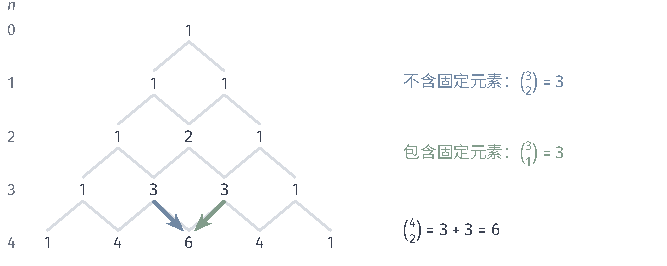
\includegraphics[width=112mm]{figures/01-mathematical-preliminaries-upper/01-mathematical-language-combinatorics-analysis-optimization/tikz/comprehension-additions/pascal-recurrence.pdf}
  \caption{组合数的逐行递推。第$n$行列出$\binom n0,\ldots,\binom nn$；箭头突出$\binom42=\binom32+\binom31=3+3$。两种分类分别从其余三个元素选两个，或先保留固定元素再从其余三个中选一个。网格位置表示递推依赖，不表示子集包含关系。}
  \label{fig:vol1-add-pascal-recurrence}
\end{figure}

\paragraph{组合数的交错和}
交错和$\sum_k(-1)^k\binom nk$把偶数大小子集的个数记为正，奇数大小子集的个数记为负。
当$n\geq1$时，固定$V$中的一个元素$i$，定义映射：若$i\in S$就把$i$删去，若$i\notin S$就把$i$加入。
这个映射作用两次回到原子集，所以是$\mathcal P(V)$到自身的双射；它每次恰好改变子集大小$1$，
因而把偶数大小的子集一一送到奇数大小的子集。两类子集个数相同，正负相抵，因而
\begin{equation}
 \sum_{k=0}^n(-1)^k\binom nk=0,\qquad n\geq1.
 \label{eq:comb-alternating-subset-count}
\end{equation}
$n=0$时只有空集，交错和为$1$。后面的容斥与Möbius反演将用这项抵消关系。

\subsubsection{子集与划分的计数}
\label{sec:comb-subset-partition-counts}

排列和组合数的是固定大小的选择。若不限制选多少个，或者要把全部对象分到几组，
仍可以先用双射换成零一记录，再用乘法规则与等倍归并计数。

\paragraph{幂集}
\phantomsection
\label{sec:comb-ordered-unordered}
若不限制子集大小，结果集合为幂集$\mathcal P(V)$，它包含$V$的所有子集。
每个子集$S$对应一条长度为$n$的零一记录$(z_1,\ldots,z_n)$：第$i$位为$1$表示$i\in S$，为$0$表示$i\notin S$。
不同子集至少在一个元素上不同，记录也就在相应位上不同；任给一条记录，取值为$1$的位置又组成一个子集。
所以这是$\mathcal P(V)$到$\{0,1\}^n$的双射，乘法规则给出
\begin{equation}
 |\mathcal P(V)|=2^n.
 \label{eq:comb-power-set-count}
\end{equation}
例如$V_0$有$16$个子集；$n=0$时，幂集只有空集这一个元素，数量为$2^0=1$。
若只允许其中部分子集，把这些允许的子集组成的集合称为
\term{集合族}（set family），记作$\mathcal F\subseteq\mathcal P(V)$，这与第~\ref{chap:sets-functions-and-proofs}章的集合族是同一概念。
例如只收集$V_0$的二元子集，就得到一个含$\binom42=6$个成员的集合族。

\paragraph{二分划分}
把$V$中的对象分到有名称的两侧，例如“已选”和“未选”，可记为$(S,V\setminus S)$。
结果由第一侧$S$唯一确定，任意$S\subseteq V$也都给出一个结果，所以允许空侧时共有$2^n$个结果。
例如把四门课分别放入“已选”和“未选”两侧，共有$16$种分法。

若两侧没有名称，交换两侧表示同一结果，这时数的是集合$\{S,V\setminus S\}$。
对$n\geq1$，$S$与$V\setminus S$总不相同，因为恰有一个包含元素$1$；
所以每个无名称结果恰有两个有名称表示，等倍归并给出$2^n/2=2^{n-1}$个。
若还要求两侧均非空，就从有名称的结果中去掉$(\varnothing,V)$与$(V,\varnothing)$两个，
有名称和无名称的数量分别为$2^n-2$与$2^{n-1}-1$。例如把四个对象分成两个无名称的非空组，共有$8-1=7$种。
$n=0$时，允许空侧只有$(\varnothing,\varnothing)$一个结果，且两侧相同；要求非空则没有结果。
这时每个无名称结果不再恰有两个表示，等倍归并的条件不成立，不能使用除以$2$的公式。

\subsection{存在重叠关系的计数}
\label{sec:comb-overlap-counting}
\label{sec:comb-inclusion-mobius}

加法规则要求类别不交。若同一元素属于多个集合，直接相加就会重复计算，需要用交集大小校正。

\paragraph{容斥原理}

设$A=\{1,2,3,4\}$、$B=\{3,4,5\}$。$|A|+|B|=4+3=7$把公共元素$3,4$都数了两次，
减去一次交集大小便得到$|A\cup B|=4+3-2=5$。
一般地，把并集分为$A\setminus B$、$A\cap B$与$B\setminus A$三个互斥区域。
加法规则给出$|A|=|A\setminus B|+|A\cap B|$、$|B|=|B\setminus A|+|A\cap B|$，
以及$|A\cup B|=|A\setminus B|+|A\cap B|+|B\setminus A|$。把前两式相加再与第三式比较，可得
\[
 |A\cup B|=|A|+|B|-|A\cap B|.
\]
图~\ref{fig:comb-inclusion-exclusion-overlap}显示需要减掉的正是公共区域多出来的一次计数。
\begin{figure}[htbp]
  \centering
  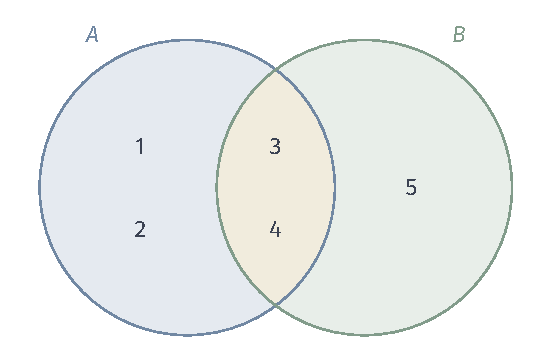
\includegraphics[width=90mm]{figures/01-mathematical-preliminaries-upper/01-mathematical-language-combinatorics-analysis-optimization/tikz/inclusion-exclusion-overlap.pdf}
  \caption{两个有限集合的重叠计数。$A=\{1,2,3,4\}$，$B=\{3,4,5\}$；仅属于$A$的区域放入$1,2$，公共区域放入$3,4$，仅属于$B$的区域放入$5$。把两圈元素个数相加时，公共区域被数两次，减去一次后得到并集中的五个不同元素。}
  \label{fig:comb-inclusion-exclusion-overlap}
\end{figure}

对三个有限集合，逐个元素检查它被计了几次。只属于一个集合的元素在$|A|+|B|+|C|$中计一次，不出现在任何交集中；
恰属于两个集合的元素先计两次，再在一个两两交集中减去一次，最终计一次；
同时属于三者的元素先计三次，在三个两两交集中各减一次后变为$3-3=0$次，
所以还要加回三重交集。因此
\[
 \begin{aligned}
 |A\cup B\cup C|&=|A|+|B|+|C|\\
 &\quad-|A\cap B|-|A\cap C|-|B\cap C|+|A\cap B\cap C|.
 \end{aligned}
\]
在上述例子加入$C=\{4,5,6\}$，两两交集大小为$2,1,2$，三重交集大小为$1$，
并集大小为$4+3+3-2-1-2+1=6$。

\term{容斥原理}（inclusion--exclusion principle）
把这种交替校正推广到任意有限个集合。
\begin{theorem}[有限容斥原理]
\label{thm:comb-inclusion-exclusion}
设$A_1,\ldots,A_m$是有限集合。则
\begin{equation}
  \left|\bigcup_{i=1}^{m}A_i\right|
  =\sum_{\varnothing\neq I\subseteq\{1,\ldots,m\}}
  (-1)^{|I|+1}\left|\bigcap_{i\in I}A_i\right|.
  \label{eq:comb-inclusion-exclusion}
\end{equation}
\end{theorem}

\begin{proof}
沿用三个集合时的思路，逐个元素比较两侧的贡献。左侧中，并集的每个元素恰计一次。
右侧是若干集合大小的带符号和；把每个$|\bigcap_{i\in I}A_i|$写成其中元素各计一次的和，
再按元素合并，就只需检查每个元素$x$在右侧的总系数。
设$x$恰好属于$r$个集合$A_i$，记这些下标组成集合$J$，$|J|=r$。
$x$属于交集$\bigcap_{i\in I}A_i$当且仅当$I\subseteq J$。$r=0$时没有这样的非空$I$，$x$也不在并集中，两侧都不计入它。
$r\geq1$时，大小为$k$的$I\subseteq J$有$\binom rk$个，每个贡献系数$(-1)^{k+1}$，所以$x$在右侧的总系数为
\[
 \sum_{k=1}^r(-1)^{k+1}\binom rk
 =-\left(\sum_{k=0}^r(-1)^k\binom rk-1\right)=1,
\]
最后一步用式~\eqref{eq:comb-alternating-subset-count}：$r\geq1$时交错和为零。
所以并集中的每个元素在右侧也恰好计入一次，两侧相等。
\end{proof}

\paragraph{补集计数}

有些限制条件同时涉及多项要求，直接数满足全部要求的结果比较困难；
不满足要求的结果却可以按“违反哪一条”分别描述。这时先数坏结果，再从总数中减去。
例如四门课的选择用$\bm z=(z_1,z_2,z_3,z_4)\in\{0,1\}^4$表示，$z_i=1$表示选第$i$门课。
要求课程$1,2$恰选一门，选$3$必须选$1$，选$4$必须选$2$或$3$中的至少一门。
违反各条规则的集合分别为
\[
 \begin{aligned}
 A_1&=\{\bm z:z_1=z_2\},\\
 A_2&=\{\bm z:z_3=1,\ z_1=0\},\\
 A_3&=\{\bm z:z_4=1,\ z_2=z_3=0\}.
 \end{aligned}
\]
由De Morgan律，满足全部规则的结果组成$A_1^{\mathrm c}\cap A_2^{\mathrm c}\cap A_3^{\mathrm c}=(A_1\cup A_2\cup A_3)^{\mathrm c}$，
所以合法结果数等于$16-|A_1\cup A_2\cup A_3|$，而后者正好用容斥原理计算。
各项大小都可以用乘法规则读出：$A_1$中$z_1=z_2$的共同取值有$2$种，$z_3,z_4$各有$2$种，故$|A_1|=8$；
$A_2$固定两位、其余两位自由，故$|A_2|=4$；$A_3$固定三位，故$|A_3|=2$。
$A_1\cap A_2$要求$z_1=z_2=0$、$z_3=1$，只剩$z_4$自由，有两个元素；
$A_1\cap A_3$要求$z_2=0$，进而$z_1=0$，又$z_3=0$、$z_4=1$，只有$(0,0,0,1)$；
$A_2\cap A_3$同时要求$z_3=1$与$z_3=0$，为空集，三重交集也就为空。
坏结果共有$8+4+2-2-1-0+0=11$个，
所以合法结果为$16-11=5$个，对应的课程集合族是
\begin{equation}
 \mathcal C_0=\bigl\{\{1\},\{1,3\},\{1,3,4\},\{2\},\{2,4\}\bigr\}.
 \label{eq:comb-running-feasible-family}
\end{equation}
直接核对也得到同样的五个：$z_1=1,z_2=0$时$z_3$可任取，但$z_4=1$要求$z_3=1$，得到三种；
$z_1=0,z_2=1$时必须$z_3=0$，$z_4$可任取，得到两种。

\subsection{Möbius反演}
\label{sec:comb-cumulative-inversion}

容斥原理由各交集的大小恢复并集的大小。类似的问题也出现在更一般的数值上：
设想四门课程组合各有一个“得分”，单门课各有贡献，某两门课同时选又会产生额外的配合效果。
我们能观察到的是每个课程组合的总得分，想知道的却是每个组合自身贡献了多少。
总得分是其全部子组合贡献的累计，恢复单个贡献就是把这种累计倒过来。
本小节先把“给子集赋值”写成集合函数，再给出反演公式并证明它。

\paragraph{集合函数}

以$V$的子集为输入的函数称为集合函数（set function）。例如实值集合函数写作$g:\mathcal P(V)\to\mathbb R$，
元素计数$g(S)=|S|$就是一例。还可以在$W=\{1,3\}$上规定
$g(\varnothing)=0$、$g(\{1\})=g(\{3\})=2$、$g(W)=7$。
这个函数为每个子集给出了实数值，其中二元集合的$7$不等于两个单项值之和，说明集合函数未必可加。
多出来的$7-2-2=3$正是$\{1,3\}$作为一个整体额外贡献的部分；下面的反演公式会把这一计算推广到任意子集。

\paragraph{子集格}

累计沿包含关系进行：$S$的累计值收集所有$T\subseteq S$的贡献。
第~\ref{sec:prelim-binary-relations}节已经说明，包含关系是幂集上的偏序。
有限集合$V$的所有子集按这一偏序排列，组成子集格。它的元素是子集，次序为
$T\subseteq S$；
两个子集的交是它们最大的公共子集，并集是包含两者的最小子集。
例如$\{1\}$与$\{3\}$均包含于$\{1,3\}$，它们的共同下方还有空集。

\paragraph{Möbius反演}

记$h(T)$为子集$T$自身的贡献，$g(S)$为所有$T\subseteq S$贡献的总和。
已知$g$时，可以用下面的\term{Möbius反演}（Möbius inversion）公式恢复$h$。
\begin{theorem}[子集格上的 Möbius 反演]
\label{thm:comb-mobius-inversion}
设$V$为有限集合，$g,h:\mathcal{P}(V)\to\mathbb{R}$满足
\begin{equation}
  g(S)=\sum_{T\subseteq S}h(T)
  \qquad\text{对每个 }S\subseteq V.
  \label{eq:comb-zeta-transform}
\end{equation}
则
\begin{equation}
  h(S)
  =
  \sum_{T\subseteq S}(-1)^{|S|-|T|}g(T).
  \label{eq:comb-mobius-inversion}
\end{equation}
反过来，由式~\eqref{eq:comb-mobius-inversion}定义$h$也会恢复
式~\eqref{eq:comb-zeta-transform}。
\end{theorem}

\begin{proof}
把式~\eqref{eq:comb-zeta-transform}代入反演式右侧。所得双重和遍历满足$R\subseteq T\subseteq S$的全部集合对$(R,T)$，
先固定外层的$T$与先固定$R$遍历的是同一批集合对，所以可以像第~\ref{sec:prelim-finite-sums-products}节的三角形求和那样交换有限求和次序，得到
\begin{align*}
  \sum_{T\subseteq S}(-1)^{|S|-|T|}g(T)
  &=
  \sum_{T\subseteq S}(-1)^{|S|-|T|}
  \sum_{R\subseteq T}h(R)\\
  &=
  \sum_{R\subseteq S}h(R)
  \sum_{T:R\subseteq T\subseteq S}
  (-1)^{|S|-|T|}.
\end{align*}
固定$R$后，满足$R\subseteq T\subseteq S$的集合$T$由$S\setminus R$中哪些元素被加入决定，
即$T=R\cup D$，其中$D\subseteq S\setminus R$可以任意选取，且$|S|-|T|=|S\setminus R|-|D|$。
记$q=|S\setminus R|$，按$|D|=j$分类，大小为$j$的$D$有$\binom qj$个，内层和等于
\[
  \sum_{j=0}^{q}\binom{q}{j}(-1)^{q-j}
  =(-1)^q\sum_{j=0}^q(-1)^j\binom qj
  =\begin{cases}1,&q=0,\\0,&q\geq1,\end{cases}
\]
最后一步用式~\eqref{eq:comb-alternating-subset-count}。
它在$R=S$时为$1$，在$R\neq S$时为$0$，所以全部较小子集的贡献抵消，只留下
$h(S)$。反方向也可直接核对：由反演式定义$h$后，
\[
 \sum_{T\subseteq S}h(T)
 =\sum_{R\subseteq S}g(R)
   \sum_{T:R\subseteq T\subseteq S}(-1)^{|T|-|R|}
 =g(S).
\]
两次内层求和都使用组合数交错和的配对抵消：只有$R=S$时剩一个空集项，其余情形为零。
\end{proof}

\paragraph{反演的算例}

记$\mathbb I\{\text{条件}\}$在条件成立时取$1$，否则取$0$。
下面在$V_0$上取一个教学例子，逐项核对反演公式
\[
 g(S)=2|S|+3\mathbb I\{\{1,3\}\subseteq S\}-\mathbb I\{\{2,4\}\subseteq S\}.
\]
四个单项各贡献$2$，子集$\{1,3\}$另加$3$，子集$\{2,4\}$另加$-1$。
表~\ref{tab:comb-four-element-mobius}列出全部累计值及恢复的贡献。
\begin{table}[htbp]
  \centering
  \begin{tabular}{ccc@{\qquad}ccc}
    \toprule
    $S$ & $g(S)$ & $h(S)$ & $S$ & $g(S)$ & $h(S)$ \\
    \midrule
    $\varnothing$ & $0$ & $0$ & $\{1,2\}$ & $4$ & $0$ \\
    $\{1\}$ & $2$ & $2$ & $\{1,3\}$ & $7$ & $3$ \\
    $\{2\}$ & $2$ & $2$ & $\{1,4\}$ & $4$ & $0$ \\
    $\{3\}$ & $2$ & $2$ & $\{2,3\}$ & $4$ & $0$ \\
    $\{4\}$ & $2$ & $2$ & $\{2,4\}$ & $3$ & $-1$ \\
    $\{3,4\}$ & $4$ & $0$ & $\{1,2,3\}$ & $9$ & $0$ \\
    $\{1,2,4\}$ & $5$ & $0$ & $\{1,3,4\}$ & $9$ & $0$ \\
    $\{2,3,4\}$ & $5$ & $0$ & $V_0$ & $10$ & $0$ \\
    \bottomrule
  \end{tabular}
  \caption{四元素子集格上的累计值与局部贡献。除四个单项、交互
  $\{1,3\}$和$\{2,4\}$外，其余局部贡献均为零。}
  \label{tab:comb-four-element-mobius}
\end{table}

例如$g(\{1,3\})=7$，减去两个单项累计值并加回空集基准，得到
\[
 h(\{1,3\})=7-2-2+0=3.
\]
同样，$h(\{2,4\})=3-2-2+0=-1$。对$S=\{1,2,3\}$，
\[
 h(S)=9-(4+7+4)+6-0=0.
\]
图~\ref{fig:comb-mobius-cumulative-local}比较$\{1,3\}$的四个子集上的累计值与自身贡献。
\begin{figure}[htbp]
  \centering
  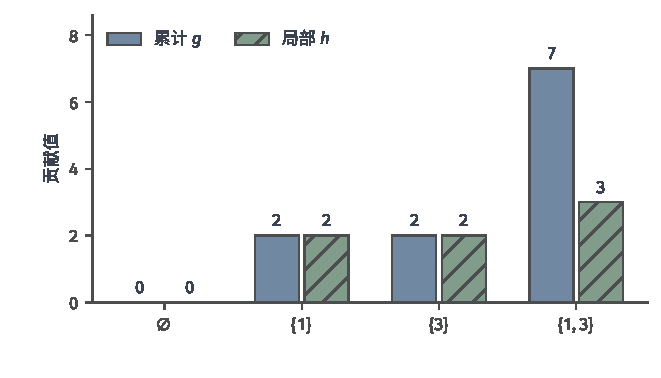
\includegraphics[width=112.0mm]{figures/01-mathematical-preliminaries-upper/01-mathematical-language-combinatorics-analysis-optimization/matplotlib/comb-mobius-cumulative-local/figure.pdf}
  \caption{同一四元素教学构造在$\{1,3\}$的子集上的累计值与局部贡献。左侧蓝柱为$g$，右侧绿斜纹柱为$h$；
 单项贡献各为$2$，二元累计值$7$包含额外交互$3$。图中四个子集的数据由正文解析式精确计算，
 没有省略影响这个二元交互的子集。}
 \label{fig:comb-mobius-cumulative-local}
\end{figure}

反演允许正、负贡献。它与容斥都使用二项式系数的交替抵消，
但容斥保留并集中的每个元素，反演保留指定子集自身的贡献。

\paragraph{Möbius函数}

反演公式中的系数$(-1)^{|S|-|T|}$只依赖两个子集的相对位置。
同样的“由累计值恢复贡献”问题也可以在任意有限偏序集上提出，这时系数由Möbius函数给出。
它由$\mu(S,S)=1$及
\[
 \mu(T,S)=-\sum_{T\preceq R\prec S}\mu(T,R)\qquad(T\prec S)
\]
递归定义，不满足$T\preceq S$时取$0$；这里$\preceq$表示偏序，$\prec$表示偏序且不相等。
递归式的含义是：对每个$S\succ T$，从$T$到$S$之间全部系数之和为零，这正是证明中内层和需要的抵消。
在子集格上，$\mu(T,S)=(-1)^{|S|-|T|}$满足这一递归：对$T\subsetneq S$，记$q=|S\setminus T|\geq1$，
则$\sum_{T\subseteq R\subseteq S}(-1)^{|R|-|T|}=\sum_{j=0}^q(-1)^j\binom qj=0$，
移项正是递归式。所以子集格上的反演系数只取正负一，与定理~\ref{thm:comb-mobius-inversion}一致。

\FloatBarrier
\section{有限输入上的可区分模式}
\label{sec:comb-label-family-capacity}

第~\ref{sec:prelim-function-families}节把候选规则组织成函数族。用观测数据挑选规则时，
我们只看得到每条规则在有限个观测输入上的输出；两条规则若在这些输入上输出相同，数据就无法区分它们。
函数类可以包含无限多个函数，但观察有限个输入时，不同函数给出的输出记录只有有限种，可以用上一节的方法计数。
本节把这些记录称为输出模式，研究两个问题：在给定个数的输入上最多能实现多少种模式；
以及最多能在多少个输入上任意指定输出。前者衡量函数类在有限数据上的区分能力，后者把这种能力概括为一个整数。
二值输出先给出限制类、生长函数和VC维；多分类输出的标签多于两个，改变一个输出有多种选择，需要区分替代标签的要求；
实值输出则先与固定阈值比较，再考虑离阈值的间隔。

\subsection{二值函数类}
\label{sec:comb-vc-growth}

固定非空输入空间$\mathcal X$与非空函数类$\mathcal H\subseteq\{0,1\}^{\mathcal X}$，
这里$\{0,1\}^{\mathcal X}$是第~\ref{sec:prelim-function-definition}节记号下全部$\mathcal X\to\{0,1\}$函数组成的集合。
每个函数在输入处只输出$0$或$1$，例如判断一封邮件是否为垃圾邮件。以下先固定输入，再比较不同输入上的模式数量。

\subsubsection{生长函数}
\label{sec:comb-binary-restrictions}

\paragraph{限制类}

先把观察范围限制在一组固定输入上，只保留函数在这些位置的输出。这样，即使原函数类无限大，当前可以区分的输出记录仍可能只有有限种。

\begin{definition}[限制类]
设$C=\{x_1,\ldots,x_m\}$为互异输入组成的有限集，并固定所列次序。
把每个函数在这些输入上的取值组成一个向量，所有这样的向量构成限制类（restriction）：
\[
 \mathcal H|_C=\{(h(x_1),\ldots,h(x_m)):h\in\mathcal H\}.
\]
\end{definition}
一个向量是一个可实现的输出模式。不同函数若在$C$上取值相同，只在限制类中计一次。
限制类是$\{0,1\}^m$的子集，所以由乘法规则至多有$2^m$个模式，无论$\mathcal H$本身有多大。
例如取$\mathcal X=\mathbb R$，令$\mathcal H=\{h_a:a\in\mathbb R\}$，
其中阈值函数$h_a(x)=\mathbb I\{x\geq a\}$把阈值右侧标为$1$，左侧标为$0$；
这里$\mathbb I\{\text{条件}\}$在条件成立时取$1$，否则取$0$。
在输入$1,2,3$上，模式只取决于阈值$a$落在哪一段：$a\leq1$时为$111$，$1<a\leq2$时为$011$，
$2<a\leq3$时为$001$，$a>3$时为$000$。所以其限制类只有这四个模式，$8$种零一记录中有一半无法实现。
$a=1.5$与$a=1.8$都产生$011$，但在输入$1.7$上取值不同，所以当前模式相同不等于函数相同。

\paragraph{生长函数}

限制类的大小取决于输入位置。固定输入个数后，对所有输入组取最大的模式数，得到生长函数。
\begin{definition}[生长函数]
  \label{def:growth-function}
  生长函数（growth function）记录$m$个输入上最多能区分多少模式。
  对整数\(m\geq0\)，定义
  \begin{equation}
    \Pi_{\mathcal H}(m)
    =\max_{x_1,\ldots,x_m\in\mathcal X}
    |\{(h(x_1),\ldots,h(x_m)):h\in\mathcal H\}|.
    \label{eq:growth-function}
  \end{equation}
  \(m=0\)时只有一个空标记，故\(\Pi_{\mathcal H}(0)=1\)。
\end{definition}

这里允许输入重复，因此有限输入空间也能讨论任意$m$；重复位置必须取得相同标签。
模式数是$1$到$2^m$之间的整数（函数类非空，所以至少有一个模式），有限个整数中总有最大者，
即使输入组有无限多种，可能取到的模式数也只有这些整数，所以定义中的最大值存在。
对阈值函数类，把$m$个互异点从小到大排为$x_1<\cdots<x_m$，模式由阈值落在
$(-\infty,x_1],(x_1,x_2],\ldots,(x_{m-1},x_m],(x_m,\infty)$中哪一段决定，
共$m+1$段，每段给出不同的模式；输入有重复时互异点更少，模式也更少。故$\Pi_{\mathcal H}(m)=m+1$。
例如$m=3$时，恰是前面的四种模式。

\paragraph{指示函数}

二值函数与子集一一对应：函数$h$确定了取值为$1$的输入组成的集合$h^{-1}(\{1\})$，
反过来，给定$S\subseteq\mathcal X$，函数$\mathbb I_S(x)=\mathbb I\{x\in S\}$称为$S$的\term{指示函数}（indicator function）：
它在$S$上取$1$，在$S$外取$0$。因此限制类中的模式也可以看作$C$的子集，即标为$1$的输入组成的集合，
生长函数就可以用有限子集计数求出。
设$\mathcal X$为无限集，固定整数$k\geq0$，令
\[
 \mathcal H_k=\{\mathbb I_S:S\subseteq\mathcal X,\ |S|\leq k\}.
\]
在$m$个互异输入上，正标签位置可以是任意大小不超过$k$的子集，因此
\[
 \Pi_{\mathcal H_k}(m)=\sum_{j=0}^{\min\{k,m\}}\binom mj.
\]
例如$k=1,m=3$时只有$000,100,010,001$，数量为$1+3=4$。
这里统计的是模式数，没有给这些模式规定概率。

\subsubsection{VC维}
\label{sec:comb-binary-shattering-counts}

\paragraph{打散}

若一组输入的全部二值模式都能实现，就可以在这些输入上任意指定标签。
\begin{definition}[打散]
  \label{def:shattering}
  若对有限互异输入集\(C\)的每个二值标记\((b_1,\ldots,b_m)\)，都存在\(h\in\mathcal H\)满足\(h(x_i)=b_i\)对全部\(i\)成立，就称\(\mathcal H\)\term{打散}（shatter）\(C\)。等价地，\(\mathcal H|_C=\{0,1\}^m\)。
\end{definition}

例如阈值函数能在一个点上实现$0$和$1$，所以能打散单点集。
在$x_1<x_2$上却不能实现$10$：若$x_1\geq a$，必有$x_2\geq a$。
因此任意两个点都不能被阈值函数类打散。

\paragraph{VC维}

VC维把能够被打散的输入集大小概括为一个数。
\begin{definition}[VC维]
  \label{def:vc-dimension}
  \(\mathcal H\)的\term{VC维}（Vapnik--Chervonenkis dimension）为
  \[
    \operatorname{VC}(\mathcal H)
    =\sup\{|C|:C\subseteq\mathcal X,\ |C|<\infty,\ C\text{被}\mathcal H\text{打散}\}.
  \]
  空集总能被非空函数类打散，所以维度可为\(0\)；若任意大有限集都能被打散，则取值为\(+\infty\)。
\end{definition}

由刚才的单点与两点判断，阈值函数类的VC维为$1$。
这个数记录可被任意标记的输入数，不是参数个数：
$h_{a,b}(x)=\mathbb I\{x\geq a+b\}$虽写成两个参数，仍是同一个阈值函数类，VC维仍为$1$。

\paragraph{区间指示函数}

此例取$\mathcal X=\mathbb R$、$\mathcal H=\{h_{a,b}:a,b\in\mathbb R,\ a\leq b\}$，
其中$h_{a,b}(x)=\mathbb I\{a\leq x\leq b\}$。
对$x_1<\cdots<x_m$，非空正标签位置只能是连续块$\{i,i+1,\ldots,j\}$。
每个连续块都可由区间选出，再加上全零模式，得到
\[
 \Pi_{\mathcal H}(m)=1+\sum_{i=1}^m(m-i+1)=1+\frac{m(m+1)}2.
\]
两个点的四种模式均可实现；三个点却不能实现$101$，因为包含两端的区间也包含中点。
所以区间函数类的VC维为$2$。图~\ref{fig:comb-interval-shattering-patterns}显示这两项判断。
\begin{figure}[htbp]
  \centering
  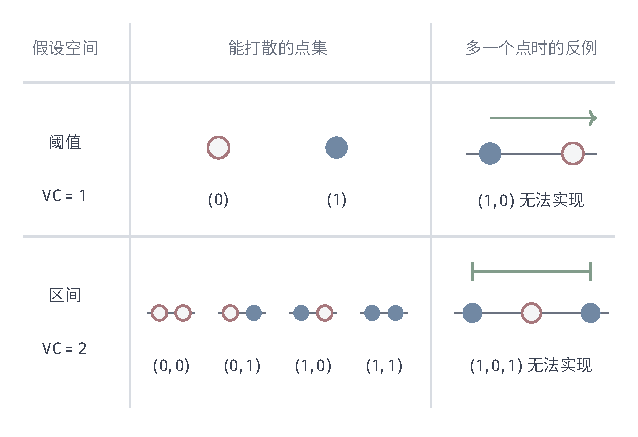
\includegraphics[width=107.999mm]{figures/01-mathematical-preliminaries-upper/01-mathematical-language-combinatorics-analysis-optimization/tikz/comb-interval-shattering-patterns/figure.pdf}
  \caption{阈值与单区间函数类的VC维。中列给出能够打散的输入和相应模式；
 右列给出多一个输入时无法实现的模式。实心点表示标签$1$，空心点表示标签$0$；
 箭头表示阈值的正标签向右延续，线段表示包含两个端点的区间也包含中间点。}
 \label{fig:comb-interval-shattering-patterns}
 \label{fig:learning-vc-shattering}
 \label{fig:learning-vc-dimension-examples}
\end{figure}

图~\ref{fig:combinatorics-growth-patterns}比较区间类的模式数与全部$2^m$个二值模式。
计数相同不要求模式相同：$\mathcal H_2$也有$1+m(m+1)/2$个模式，
但在三个点上缺少$111$，区间类缺少的是$101$。
\begin{figure}[htbp]
  \centering
  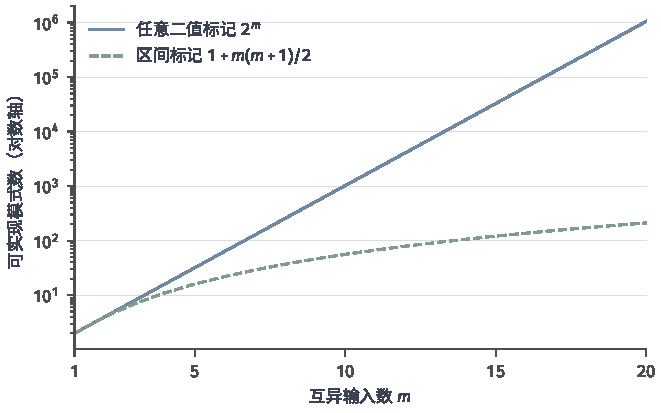
\includegraphics[width=112.0mm]{figures/01-mathematical-preliminaries-upper/01-mathematical-language-combinatorics-analysis-optimization/matplotlib/combinatorics-growth-patterns/figure.pdf}
  \caption{有限输入上的二值模式数（精确计数教学图）。蓝实线为不受限制的\(2^m\)，绿虚线为实数轴区间分类器的\(1+m(m+1)/2\)。纵轴使用对数刻度，绿线是该具体类的精确计数；它也恰等于至多两个正类点的集合族计数，但两类实现的模式可以不同。}
  \label{fig:combinatorics-growth-patterns}
  \label{fig:learning-sauer-growth}
\end{figure}

\FloatBarrier
\Needspace{16\baselineskip}
\paragraph{Sauer--Shelah引理}

阈值类和区间类的模式数都只随$m$多项式增长，远小于$2^m$；它们的VC维也都有限。
这不是巧合：只要VC维有限，生长函数就被一个关于$m$的多项式控制。
为了证明这一点，我们把问题从函数类移到有限的模式族上。
固定输入$x_1,\ldots,x_m$后，限制类是一个模式族$\mathcal A\subseteq\{0,1\}^m$。
称$\mathcal A$打散坐标集$I\subseteq\{1,\ldots,m\}$，是指$\mathcal A$中的模式在$I$的坐标上能实现全部$2^{|I|}$种取值；
$\mathcal H$打散输入$\{x_i:i\in I\}$，恰好意味着限制类打散坐标集$I$。
下面的界由删除最后一个坐标后的分类得到。
\begin{lemma}[Sauer--Shelah引理]
  \label{lem:sauer-shelah}
  若\(d=\operatorname{VC}(\mathcal H)<\infty\)，则对任意\(m\geq0\)，
  \[
    \Pi_{\mathcal H}(m)\leq\sum_{j=0}^{\min\{d,m\}}\binom mj.
  \]
  特别地，当\(1\leq d\leq m\)时，
  \begin{equation}
    \Pi_{\mathcal H}(m)\leq\sum_{j=0}^{d}\binom mj
    \leq\left(\frac{em}{d}\right)^d.
    \label{eq:sauer-shelah}
  \end{equation}
\end{lemma}

\begin{proof}
记$\Phi(m,d)=\sum_{j=0}^{\min\{d,m\}}\binom mj$。我们证明更一般的命题：
任何不能打散超过$d$个坐标的模式族$\mathcal A\subseteq\{0,1\}^m$都满足$|\mathcal A|\leq\Phi(m,d)$。
对$\mathcal H$的任一输入组，限制类不能打散超过$d$个坐标（否则相应输入被$\mathcal H$打散，与VC维为$d$矛盾），
所以这个命题给出引理的第一项结论。

先处理边界情形。$m=0$时只有空模式，$|\mathcal A|\leq1=\Phi(0,d)$。
$d=0$时$\mathcal A$不能打散任何单个坐标；若$\mathcal A$含有两个不同模式，它们在某一坐标上分别取$0$和$1$，
就打散了这个坐标，所以$|\mathcal A|\leq1=\Phi(m,0)$。

对$m,d\geq1$，假定命题对$m-1$个坐标、任意维数上界都成立。
把每个模式删去末坐标，所得前缀组成$U\subseteq\{0,1\}^{m-1}$；
令$W\subseteq U$为既能接$0$又能接$1$的前缀，即$u0$与$u1$都属于$\mathcal A$的前缀$u$。
按前缀给$\mathcal A$的模式分类：每个前缀$u\in U$对应一个或两个模式，恰在$u\in W$时对应两个。
加法规则给出$|\mathcal A|=|U|+|W|$。

$U$不能打散超过$d$个坐标：若$U$打散坐标集$I$，则$\mathcal A$中的模式在$I$上也实现全部取值，故$|I|\leq d$。
$W$不能打散$d$个坐标：若$W$打散某个$|I|=d$的坐标集，则对$I$上的任意取值，都有$W$中的前缀实现它，
而该前缀接$0$或接$1$都在$\mathcal A$中，于是$\mathcal A$打散$I\cup\{m\}$这$d+1$个坐标，产生矛盾。
所以$W$不能打散超过$d-1$个坐标。对$U$与$W$分别使用归纳假设，再用Pascal恒等式逐项合并，便得到
\[
  |\mathcal A|
  \leq\sum_{j=0}^{d}\binom{m-1}{j}
       +\sum_{j=0}^{d-1}\binom{m-1}{j}
  =\binom{m-1}0+\sum_{j=1}^{d}\left[\binom{m-1}j+\binom{m-1}{j-1}\right]
  =\sum_{j=0}^{d}\binom mj,
\]
其中超过坐标数的组合数约定为零，因此这也等于$\Phi(m,d)$。重复输入只会减少可独立取值的坐标，不会增大模式数，
因此对全部输入组取最大值得到第一项结论。

简化界另用初等指数不等式$1+u\leq e^u$（$u\geq0$），其中$e$为自然指数的底；
这一不等式将在第~\ref{chap:function-limits}章由指数函数的级数构造直接读出。
它把有限二项式和写成便于比较的上界，前面的二项式和结论不依赖这一步。
还要比较$\sum_j\binom mja^j$与$(1+a)^m$：把$m$个因子$(1+a)$的乘积逐项展开，
每一项从每个因子中选$1$或$a$；按选出$a$的因子组成的集合分类，选出$j$个$a$的方式恰有$\binom mj$种，每种贡献$a^j$。
因此$\sum_{j=0}^m\binom mja^j=(1+a)^m$，舍去$j>d$的非负项便得下式中的第二个不等号。
当\(1\leq d\leq m\)时，令\(a=d/m\in(0,1]\)。对\(j\leq d\)有\(a^d\leq a^j\)，故
\[
  a^d\sum_{j=0}^{d}\binom mj
  \leq\sum_{j=0}^{d}\binom mj a^j
  \leq(1+a)^m\leq e^{am}=e^d.
\]
除以\(a^d=(d/m)^d\)便得到简化界。\(d=0\)时第一项界为\(1\)，不使用含\(d\)作分母的简化式。
\end{proof}

例如$d=2$时，上界为$1+m+\binom m2$，区间函数类恰好达到它。
这个引理是计数结论；将它用于抽样误差，还需要概率、可测性等条件，
可参考\BookChapterRef{chap:random-sequences-and-processes}{卷2《数学准备：概率、因果与决策》的“随机序列与随机过程”章}。

\subsection{多分类函数类}
\label{sec:comb-multiclass-dimensions}

固定非空输入集合$X$、非空标签集合$Y$和非空函数类$\mathcal H\subseteq Y^X$。
限制类仍记录有限互异输入上的输出向量。二值情形下，打散要求每个输入都能取“另一个”标签，
而另一个标签是唯一的。标签超过两个时，改变一个标签有多种选择，“任意安排输出”就有不同的严格程度：
可以要求在事先固定的两个标签之间任选，可以要求每个模式都能单独改动任一坐标，
也可以只要求能任意决定每个输入是否等于某个参照标签。
下面依次给出这三种要求及相应维数，它们对替代标签的限制由强到弱，最后比较三者的大小关系。

\subsubsection{Natarajan维}
\label{sec:comb-fixed-label-pairs}

\paragraph{Natarajan打散}

Natarajan打散在每个输入上预先固定两个不同标签，再要求实现全部逐点二选一组合。
设$C=\{x_1,\ldots,x_m\}\subseteq X$。若存在$f,g:C\to Y$，
满足每个$x$上$f(x)\neq g(x)$，且对每个$B\subseteq C$都有$h_B\in\mathcal H$满足
\begin{equation}
 h_B(x)=\begin{cases}f(x),&x\in B,\\g(x),&x\in C\setminus B,\end{cases}
 \label{eq:natarajan-shattering}
\end{equation}
就称$C$被$\mathcal H$ \term{Natarajan打散}（Natarajan shattering）。
例如两个输入分别固定标签对$(a,b)$、$(u,v)$时，需要
$(a,u),(a,v),(b,u),(b,v)$四种模式全部出现。

\paragraph{Natarajan维}

固定标签对以后，可以逐个检查哪些输入集允许全部二选一安排。将这些输入集的大小汇总，就得到函数类在这种要求下的维数。

\begin{definition}[Natarajan维]
\label{def:natarajan-dimension}
$\mathcal H$的Natarajan维（Natarajan dimension）为
\[
 d_N(\mathcal H)=\sup\{|C|:C\subseteq X\text{为被}\mathcal H\text{ Natarajan打散的有限集}\}.
\]
没有非空被打散集合时取$0$，可打散任意大有限集时取$+\infty$。
\end{definition}

二标签时，每点的两种标签就是整个$Y$，所以Natarajan维等于VC维。
下面的三标签例子可以逐项检查定义中的四种选择。
\begin{example}[Natarajan维恰为2的有限函数类]
\label{ex:comb-natarajan-concrete}
令输入空间为三封固定邮件$x_1,x_2,x_3$，函数类只含
图~\ref{fig:natarajan-concrete}中的四个函数。在$x_1$上固定标签对“正常、广告”，
在$x_2$上固定“正常、诈骗”，四个函数实现两对标签的全部四种逐点选择，所以
$d_N\geq2$。第三封邮件在四个函数下都预测为正常，任何包含$x_3$的输入集都不能
在该处实现两个不同标签；输入空间只有三点，因此$d_N\leq2$。两项合起来得到
$d_N=2$。
\end{example}

\begin{figure}[htbp]
  \centering
  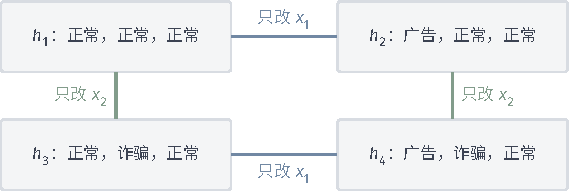
\includegraphics[width=96.28mm]{figures/01-mathematical-preliminaries-upper/01-mathematical-language-combinatorics-analysis-optimization/tikz/natarajan-concrete/figure.pdf}
  \caption{Natarajan打散的四种预测。每个框中的三项依次对应$x_1,x_2,x_3$；
 横向只改变$x_1$，纵向只改变$x_2$，而$x_3$始终预测为正常。
 每个输入处的两个标签预先固定，四个函数实现全部二选一组合。}
 \label{fig:natarajan-concrete}
\end{figure}
\FloatBarrier

\paragraph{生长函数}

当$|Y|=K<\infty$时，沿用式~\eqref{eq:growth-function}对所有输入组取最大值，
定义多分类生长函数$\Pi_{\mathcal H}(m)$，它至多为$K^m$。
有限Natarajan维可将这一上界改进为下面的二项式和。
\begin{theorem}[有限标签的预测数目上界]
\label{thm:multiclass-growth-bound}
设\(2\leq |Y|=K<\infty\)，\(d=d_N(\mathcal H)<\infty\)。
记\(q=\binom K2=K(K-1)/2\)为不同无序标签对的数目，则对每个整数\(m\geq0\)，
\begin{equation}
  \Pi_{\mathcal H}(m)\leq G_{d,K}(m)
  :=\sum_{j=0}^{\min\{d,m\}}\binom mj q^j.
  \label{eq:comb-multiclass-growth-bound}
\end{equation}
\end{theorem}

\begin{proof}
将有限非空模式族\(V\subseteq Y^m\)视为坐标集\(\{1,\ldots,m\}\)上的函数类，
并设其Natarajan维至多为\(d\)。删去末坐标得到前缀族\(U\subseteq Y^{m-1}\)。
对\(u\in U\)，记它能够接上的末尾标签数为\(r(u)\geq1\)。按前缀分类，\(|V|=\sum_{u\in U}r(u)\)，
而\(|U|=\sum_{u\in U}1\)，所以\(|V|-|U|=\sum_u(r(u)-1)\)。
对每个不同标签对\(\{a,b\}\)，令\(U_{a,b}\)为既能接上\(a\)又能接上\(b\)的前缀族。
一个前缀属于\(U_{a,b}\)，当且仅当\(\{a,b\}\)是它能接上的\(r(u)\)个标签中的一对，所以它恰属于\(\binom{r(u)}2\)个\(U_{a,b}\)，
即\(\sum_{\{a,b\}}|U_{a,b}|=\sum_u\binom{r(u)}2\)。又因\(r\geq1\)时\(r-1\leq r(r-1)/2=\binom r2\)，对前缀求和可得
\[
  |V|\leq |U|+\sum_{\substack{\{a,b\}\subseteq Y\\a\neq b}}|U_{a,b}|.
\]
每个无序对在求和中只出现一次。\(U\)的Natarajan维至多为\(d\)。当\(d\geq1\)
时，每个非空\(U_{a,b}\)的Natarajan维至多为\(d-1\)：否则它可以在某\(d\)个
坐标上实现全部固定标签对的选择；每个对应前缀又能接上\(a\)或\(b\)，使\(V\)
在这\(d\)个坐标与末坐标上实现全部二元选择，违反维度上界。空\(U_{a,b}\)的
计数贡献为零。

记\(M(m,d)\)为Natarajan维至多\(d\)的非空模式族\(V\subseteq Y^m\)能够达到的
最大大小，标签集\(Y\)保持固定。对\(m,d\geq1\)，上述分组给出
\[
  M(m,d)\leq M(m-1,d)+qM(m-1,d-1).
\]
零个坐标只有一个空模式，故\(M(0,d)=1\)。维度为零时也至多有一个模式：两个
不同模式必在某坐标上取不同标签，从而Natarajan打散一个坐标。因此\(M(m,0)=1\)。
对\(m\)归纳，将两个较小问题的上界代入，并使用二项式递推关系，得到
\[
\begin{aligned}
  M(m,d)
  &\leq\sum_{j=0}^{d}\binom{m-1}{j}q^j
       +q\sum_{j=0}^{d-1}\binom{m-1}{j}q^j\\
  &=\sum_{j=0}^{d}\binom mj q^j,
\end{aligned}
\]
其中超出坐标数的组合数约定为零。任意输入组上的限制类，其Natarajan维不超过
\(d_N(\mathcal H)\)；重复输入不能作为两个可独立选择的坐标。因此对输入组取最大值，
得到式~\eqref{eq:comb-multiclass-growth-bound}。
\end{proof}

例如$K=3,d=1,m=4$时，$q=3$，界为$1+4\times3=13$，小于全部$3^4=81$种模式。
$K=2$时$q=1$，该公式恢复Sauer--Shelah计数界。

\subsubsection{DS维}
\label{sec:comb-coordinate-replacements}

\paragraph{伪立方体}

另一种要求是不固定标签对，而让每个模式都能单独改变任一坐标，并仍留在同一个有限模式族中。
\begin{definition}[伪立方体]
\label{def:pseudocube}
有限非空集合$V\subseteq Y^m$称为$m$维伪立方体，如果对每个$v\in V$和
每个$i\in\{1,\ldots,m\}$，都存在$u\in V$满足
$u_i\neq v_i$且$u_j=v_j$对所有$j\neq i$成立。
\end{definition}

例如取三个互异标签$a,b,c$，
\[
 \mathcal V=\{(a,a),(a,b),(b,b),(b,c),(c,c),(c,a)\}
\]
是二维伪立方体：每个模式沿第一、第二坐标都能找到一个邻居。
它却不含固定两标签对形成的四个角。图~\ref{fig:comb-multiclass-pattern-grid}把六个模式列入表格，
每行每列都有两个模式，但没有完整的二行二列矩形。
\begin{figure}[htbp]
  \centering
  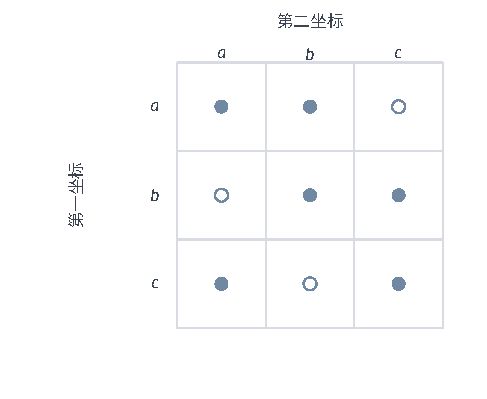
\includegraphics[width=82.501mm]{figures/01-mathematical-preliminaries-upper/01-mathematical-language-combinatorics-analysis-optimization/tikz/comb-multiclass-pattern-grid/figure.pdf}
  \caption{六模式族$\mathcal V$的精确占位图。实心点表示模式属于该族，空心点表示缺失模式。每行每列恰有两个实心点，却没有完整的四角矩形；这不是两个标签的完整立方体。}
 \label{fig:comb-multiclass-pattern-grid}
\end{figure}

\paragraph{DS打散}

若$m$个互异输入组成的有序点集$C$满足$\mathcal H|_C$包含一个$m$维伪立方体，
称$C$被\term{DS打散}（DS shattering）。例如把上述六模式作为两个输入上的全部限制类，
这两个输入便被DS打散，因为六个模式构成二维伪立方体。

\paragraph{DS维}

把能够逐坐标替换的输入规模汇总，就得到Daniely--Shalev-Shwartz维，简称DS维；
下面采用有限伪立方体的表述\scite{brukhim2022multiclass}。
\begin{definition}[DS维]
\label{def:ds-dimension}
DS维$d_{DS}(\mathcal H)$为可被DS打散的有限输入集大小的上确界。
空集给出大小$0$；若任意大的有限集都能被DS打散，维数取$+\infty$。
\end{definition}

对只有两个输入的函数类$\mathcal V$，上述六个模式构成二维伪立方体，因此$d_{DS}=2$。
没有四角矩形意味着不能Natarajan打散两个输入，而一个输入可以取不同标签，故$d_N=1$。
图~\ref{fig:ds-six-cycle}标出每个模式沿两个坐标的邻居。
\begin{figure}[htbp]
  \centering
  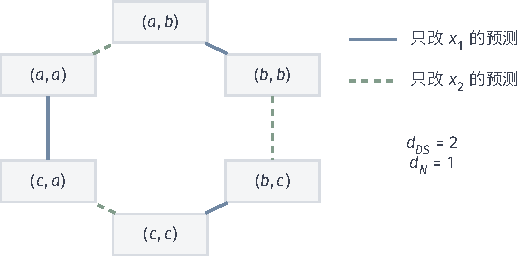
\includegraphics[width=89.02mm]{figures/01-mathematical-preliminaries-upper/01-mathematical-language-combinatorics-analysis-optimization/tikz/ds-six-cycle/figure.pdf}
  \caption{六模式族$\mathcal V$的逐坐标邻接。每个顶点是一种两输入预测；
 蓝实线只改变第一坐标，绿虚线只改变第二坐标。每个顶点在两个方向上都有邻居，
 所以它构成二维伪立方体；图中没有固定两标签对形成的四角矩形，故其
 DS维为2而Natarajan维为1。}
 \label{fig:ds-six-cycle}
\end{figure}

\subsubsection{图维}
\label{sec:comb-reference-labels}

\paragraph{图打散}

图打散先固定每点的参照标签，再要求任意一部分输入匹配参照、其余输入不匹配。
不匹配时采用哪个标签不必预先指定。
\begin{definition}[图打散]
\label{def:graph-dimension}
若有限集$C\subseteq X$存在$f:C\to Y$，使每个$B\subseteq C$都对应某个
$h_B\in\mathcal H$，满足
\[
 h_B(x)=f(x)\ (x\in B),\qquad h_B(x)\neq f(x)\ (x\in C\setminus B),
\]
则称$C$被$\mathcal H$图打散。
\end{definition}

例如参照标签为$(a,u)$时，$(a,u),(a,v),(b,u),(c,w)$分别实现全匹配、只匹配第一处、
只匹配第二处和全不匹配，其中$v\neq u$、$b,c\neq a$、$w\neq u$。

\paragraph{图维}

图打散判断一组输入能否独立安排匹配与不匹配。把能够这样安排的输入数概括为一个上界，就得到对应的维数。

\begin{definition}[图维]
\label{def:graph-dimension-value}
图维（graph dimension）记录可独立安排这种匹配关系的最大点数。
设$\mathcal C_G$为所有被$\mathcal H$图打散的有限输入集组成的集合，定义
\[
 d_G(\mathcal H)=\sup_{C\in\mathcal C_G}|C|.
\]
\end{definition}

\begin{example}[图维恰为2的有限函数类]
\label{ex:comb-graph-shattering-concrete}
令输入空间为$\{x_1,x_2,x_3\}$，函数类只含图~\ref{fig:graph-shattering-concrete}
中的四个函数。以$f(x_1)=a,f(x_2)=u$为基准，四个函数在前两个输入上分别实现
“两处都匹配、只匹配第一处、只匹配第二处、两处都不匹配”，所以
$\{x_1,x_2\}$被图打散。第三个输入始终取$z$，任何包含$x_3$的集合都不能在该处
独立安排匹配与不匹配；输入空间又只有三个点，故这个函数类的图维恰为2。
\end{example}

\begin{figure}[htbp]
  \centering
  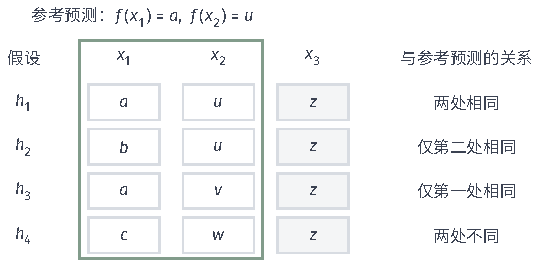
\includegraphics[width=91.401mm]{figures/01-mathematical-preliminaries-upper/01-mathematical-language-combinatorics-analysis-optimization/tikz/graph-shattering-concrete/figure.pdf}
  \caption{图打散与图维的有限例子。框线圈定的两列相对于参考函数实现全部四种匹配或
 不匹配组合；第三列固定为$z$。同一输入偏离基准时可以采用不同标签，
 因而图打散没有预先固定唯一的替代标签。}
 \label{fig:graph-shattering-concrete}
\end{figure}

\paragraph{维数比较}

三种维数分别要求固定标签对、逐坐标邻居和匹配参照标签，按对替代标签的限制由强到弱排列。
表~\ref{tab:comb-multiclass-dimensions}列出条件，图~\ref{fig:learning-multiclass-dimensions}显示对应模式。
\begin{table}[htbp]
  \centering
  \begin{tabular}{p{0.17\linewidth}p{0.70\linewidth}}
    \toprule
    维度 & 在有限输入上的要求\\
    \midrule
    Natarajan维 & 每点固定两个不同标签，全部\(2^m\)种逐点二选一组合均可实现\\
    DS维 & 包含有限非空模式族，每个模式在任一坐标都可单独改变并仍留在族中\\
    图维 & 每点固定一个基准标签，任意点集上匹配、其补集上不匹配的模式均可实现\\
    \bottomrule
  \end{tabular}
  \caption{多类别组合维度的不同量词。图维中的“图”指标记相等关系的图打散，不是输入关系图的顶点数。}
  \label{tab:comb-multiclass-dimensions}
\end{table}

\begin{figure}[htbp]
  \centering
  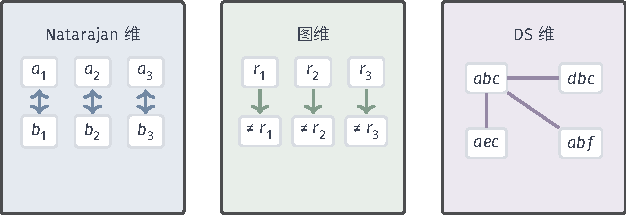
\includegraphics[width=106.056mm]{figures/01-mathematical-preliminaries-upper/01-mathematical-language-combinatorics-analysis-optimization/tikz/learning-multiclass-dimensions/figure.pdf}
  \caption{多分类维度关注的三种结构。Natarajan维固定每个输入处的两个标签，
 图维固定一个基准标签并区分匹配与不匹配，DS维考察预测向量之间只改变一个坐标的
 邻接。右栏只展示局部邻接方式；完整伪立方体还要求每个模式在每个坐标上都有邻居。}
 \label{fig:learning-multiclass-dimensions}
\end{figure}
\FloatBarrier

三种打散要求对替代标签作出的限制不同，但同一组预测模式可以同时接受这些检验。下面比较由这些要求得到的维数，并说明标签数有限时还能推出什么。

\begin{theorem}[多分类维度的比较]
\label{thm:multiclass-dimension-comparison}
对任意非空标签空间与非空函数类，有
\[
  d_N(\mathcal H)\leq d_{DS}(\mathcal H)\leq d_G(\mathcal H).
\]
二标签时三者均等于VC维。若\(|Y|=K<\infty\)，则\(d_N(\mathcal H)<\infty\)
也蕴含\(d_G(\mathcal H)<\infty\)。
\end{theorem}

\begin{proof}
若\(m\)个输入被Natarajan打散，每个坐标的两个候选标签固定，全部\(2^m\)种
选择组成一个有限非空模式族。任意模式都能只翻转任一坐标上的选择并仍留在族中，
所以它是\(m\)维伪立方体，证明\(d_N\leq d_{DS}\)。

若限制类包含\(m\)维伪立方体\(V\)，固定\(v\in V\)作为基准。任取希望偏离基准
的坐标集\(I\subseteq\{1,\ldots,m\}\)，逐个沿\(I\)中的坐标移动到邻居，每个
坐标只移动一次。每一步仅改变当前坐标；之前改变的坐标保持不变，\(I\)之外的
坐标始终与\(v\)相同。因此最终模式恰在\(I\)上不等于\(v\)，在其补集上等于
\(v\)。令\(I\)遍历所有子集就得到图打散，故\(d_{DS}\leq d_G\)。

二标签时，偏离基准的标签唯一。图打散因此要求全部二元模式；伪立方体从任意模式
逐坐标翻转也能到达全部二元模式。Natarajan打散中的两标签正是整个标签集，所以
三种维度都等于VC维。

若\(K=1\)，函数类在任何输入上只有一种标记，三种维度均为零。若\(2\leq K<\infty\)
且\(d_N=d<\infty\)，图打散\(m\)个输入至少需要\(2^m\)个不同模式。由定理~
\ref{thm:multiclass-growth-bound}，必有\(2^m\leq G_{d,K}(m)\)。固定\(d,K\)后，
当$d=0$时，右侧为$1$，所以只能有$m=0$。当$d\geq1$且$m\geq2(d+1)$时，
大小为$d+1$的子集只是全部$2^m$个子集中的一类，再利用组合数的连乘公式，可得
\[
 2^m\geq\binom m{d+1}\geq\frac{(m/2)^{d+1}}{(d+1)!},
 \qquad
 G_{d,K}(m)\leq C m^d,
\]
其中$C=\sum_{j=0}^d q^j/j!$只依赖$d,K$。与$2^m\leq G_{d,K}(m)$合并并约去$m^d$，
得到$m\leq2^{d+1}(d+1)!C$。较小的$m<2(d+1)$也已有有限上界，故图维有限。
\end{proof}

六模式族$\mathcal V$以$(a,a)$为参照时，$(a,a),(a,b),(c,a),(b,b)$实现四种匹配安排，
所以$d_G=2$。该例的三个维数依次为$1,2,2$。
有限标签条件用于计数界。例如无限标签集$Y$上的全部常值函数$h_y(x)=y$，
三个维数都为$1$，但在单个输入上已有无限多个模式，不能套用含有限$K$的计数公式。

\subsection{实值函数类}
\label{sec:comb-real-valued-threshold-margins}

以下固定非空输入空间$\mathcal X$与非空函数类$\mathcal F\subseteq\mathbb R^{\mathcal X}$。
实数输出在单点上就可能无限多；与其计数精确数值，可以先固定每个输入的阈值，
只记录输出在阈值哪一侧。加入正间隔后，还能描述在给定尺度下能否作出这些选择。

\subsubsection{伪维}
\label{sec:comb-threshold-patterns}

\paragraph{伪打散}

实值函数在单个输入上就能取无限多个值，若按精确数值计数，限制类往往无限，前面的计数没有意义。
把实数输出转化为二值信息的最直接办法，是与一个阈值比较，只记录输出在阈值上方还是下方。
对每个输入先选一个阈值，再检查全部高低组合是否可由函数实现，这称为伪打散。
阈值对全部模式保持不变，实现不同模式的函数则可以不同。
\begin{definition}[伪打散]
\label{def:pseudo-shattering}
设$\mathcal F\subseteq\mathbb R^{\mathcal X}$。有限集$C=\{x_1,\ldots,x_m\}$被
$\mathcal F$\term{伪打散}（pseudo-shattering），是指存在$r_1,\ldots,r_m\in\mathbb R$，使任意
$\bm b\in\{0,1\}^m$都对应某个$f_{\bm b}\in\mathcal F$，满足
\[
 b_i=1\Rightarrow f_{\bm b}(x_i)>r_i,\qquad
 b_i=0\Rightarrow f_{\bm b}(x_i)<r_i\quad(1\leq i\leq m).
\]
这里$\Rightarrow$表示“只要左侧条件成立，右侧便须成立”。
\end{definition}

例如取常值函数类$\mathcal F=\{f_a:a\in\mathbb R\}$，其中$f_a(x)=a$。
在一个输入处取阈值$0$，用$a=1$和$a=-1$便能实现高、低两种模式。
两个输入则不能被它伪打散：若阈值$r_1\leq r_2$，要求第一处低于$r_1$、第二处高于$r_2$，
同一个常数不可能同时满足；$r_2\leq r_1$时交换两处即可。

\paragraph{伪维}

常值函数的例子表明，可任意安排高低模式的输入数可能受到限制。伪维用一个数记录这种独立选择能够覆盖的输入规模。

\begin{definition}[伪维]
\label{def:pseudo-dimension}
$\mathcal F$的\term{伪维}（pseudo-dimension）为
$\operatorname{Pdim}(\mathcal F)=\sup\{|C|:C\text{为被}\mathcal F\text{伪打散的有限集}\}$，
允许值为$+\infty$；没有非空被打散集合时值为$0$。
\end{definition}

由刚才的一点、两点判断，常值实函数类的伪维为$1$。
对二值函数类取阈值$1/2$，伪打散就是VC打散，因此伪维与VC维一致。

\subsubsection{胖打散维}
\label{sec:comb-margin-patterns}

\paragraph{胖打散}

\term{胖打散}（fat shattering）要求输出不仅位于阈值两侧，还要与阈值相距至少一个给定正数$\gamma$。
\begin{definition}[胖打散]
\label{def:fat-shattering}
给定$\gamma>0$，若有限集$C=\{x_1,\ldots,x_m\}$存在固定阈值$r_1,\ldots,r_m$，
使任意$\bm b\in\{0,1\}^m$均对应$f_{\bm b}\in\mathcal F$满足
\begin{equation}
 b_i=1\Rightarrow f_{\bm b}(x_i)\geq r_i+\gamma,\qquad
 b_i=0\Rightarrow f_{\bm b}(x_i)\leq r_i-\gamma,
 \label{eq:fat-shattering}
\end{equation}
则称$C$在尺度$\gamma$下被$\mathcal F$胖打散。
等价地，以$\sigma_i=2b_i-1$编码，可写为
\begin{equation}
 \sigma_i\bigl(f_{\bm\sigma}(x_i)-r_i\bigr)\geq\gamma
 \quad(i=1,\ldots,m).
 \label{eq:functional-fat-shattering}
\end{equation}
\end{definition}

例如输入空间只有一个点，函数类在该点的输出只能取$19.999$和$20.001$，固定阈值$20$。
它能实现高、低两种模式，并能留下间隔$\gamma=0.001$，却不能留下间隔$1$。
这说明跨过阈值和以给定幅度跨过阈值是不同要求。

\paragraph{胖打散维}

同一函数类在不同间隔要求下，能够独立安排的输入数可能不同。固定尺度后，再汇总所有满足胖打散要求的输入集大小，就得到相应的维数。

\begin{definition}[胖打散维]
\label{def:fat-shattering-dimension}
尺度$\gamma$下的\term{胖打散维}（fat-shattering dimension）为
$\operatorname{fat}_\gamma(\mathcal F)=
\sup\{|C|:C\text{为在尺度}\gamma\text{下被}\mathcal F\text{胖打散的有限集}\}$。
采用与伪维相同的$0$及$+\infty$约定。
\end{definition}

固定尺度后，胖打散维记录能同时满足该间隔要求的输入数目。
例如上面只有两个常值输出的函数类，在$0<\gamma\leq0.001$时维数为$1$，在$\gamma>0.001$时为$0$。

\paragraph{单调性}

增大$\gamma$只会加强要求，所以$\operatorname{fat}_\gamma(\mathcal F)$关于$\gamma$单调不增。
因$\gamma>0$保证每个见证严格位于阈值一侧，还得到
$\operatorname{fat}_\gamma(\mathcal F)\leq\operatorname{Pdim}(\mathcal F)$。
反过来，一个被伪打散的固定有限集，在某个正尺度下也被胖打散：
从有限种模式各选一个见证函数，取它们在各输入处距阈值的最小距离即可。
这个距离为正，但依赖输入集和所选函数，不能替代预先指定的尺度。

\Needspace{8\baselineskip}
\paragraph{分块常值函数}

下面用可以直接计算的函数类说明幅度限制的作用。
\begin{example}[分块常值函数的胖打散维]
\label{ex:comb-piecewise-constant-fat-dimension}
设非空集合$A_1,\ldots,A_m$构成$\mathcal{X}$的一个划分，并令
\[
  \mathcal{F}_B
  =
  \left\{
    \sum_{j=1}^{m}a_j\mathbb{I}_{A_j}:
    |a_j|\leq B
  \right\},
  \qquad B>0.
\]
当$0<\gamma\leq B$时，从每个$A_j$选一点并取阈值$r_j=0$；对任意符号模式令
$a_j=\gamma\sigma_j$，便能以间隔$\gamma$实现该模式，所以这$m$个点被胖打散。反过来，
任意$m+1$个点中至少两个落在同一个$A_j$内，而类中每个函数在这两个点取值相同。若二者
的阈值为$r$与$r'$且能够被胖打散，模式$(+1,-1)$要求$r'-r\geq2\gamma$，模式
$(-1,+1)$又要求$r-r'\geq2\gamma$，二者矛盾。因此该尺度下的胖打散维恰为$m$。
当$\gamma>B$时，
单点上的两个符号也要求函数值之差至少为$2\gamma$，超过允许区间$[-B,B]$的宽度$2B$，
故胖打散维为$0$。这个算例把分区数控制的自由方向与系数上界控制的可分辨幅度分开了。
\end{example}

图~\ref{fig:comb-fat-margin-output-square}取两个分块、$B=1$，
把两处输出表示为平面中的一个点。四种高低模式能否实现，取决于间隔区域是否仍与允许的正方形相交。
\begin{figure*}[htbp]
  \centering
  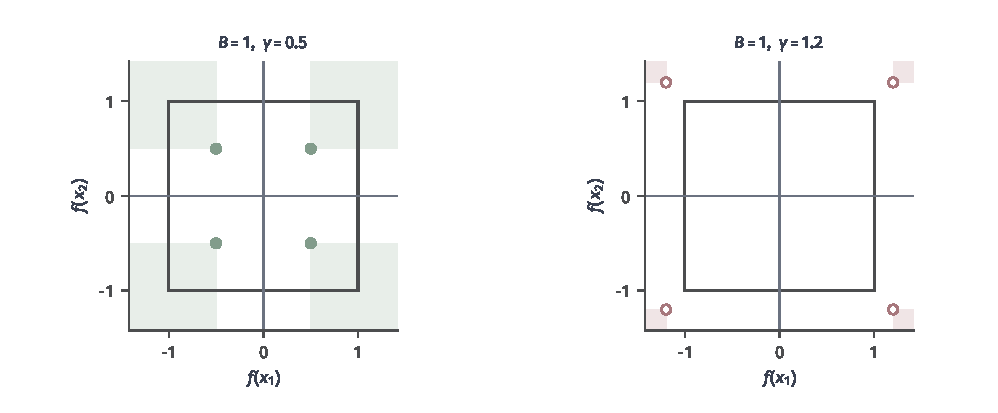
\includegraphics[width=169.0mm]{figures/01-mathematical-preliminaries-upper/01-mathematical-language-combinatorics-analysis-optimization/matplotlib/comb-fat-margin-output-square/figure.pdf}
  \caption{两个分块、$B=1$与固定阈值$r_1=r_2=0$的输出几何。灰框是函数类允许的
 $(f(x_1),f(x_2))\in[-1,1]^2$；浅色区域要求两坐标分别离阈值至少$\gamma$。
 左图的浅绿区域对应$\gamma=0.5$，四种符号可由实心点实现；右图的浅红区域对应$\gamma=1.2$，空心点只标出要求的边界，
 全部落在允许框之外，因而不是类中的函数输出。图为解析教学构造。}
 \label{fig:comb-fat-margin-output-square}
 \label{fig:fat-shattering-example}
\end{figure*}

限制类记录具体模式，生长函数记录模式数，打散维数记录满足相应打散条件的输入规模。
实值函数的伪维与胖打散维分别采用固定阈值和正间隔。
它们与函数空间中的距离、覆盖数是不同概念；后者可参考第~\ref{chap:functional-analysis-and-approximation}章。

\section{本章小结}
\label{sec:comb-summary}

有限计数首先要确定结果的身份：排列保留次序，组合只记录子集，分组还要说明各部分是否有名称。
所有计数都建立在三条规则上：双射把难数的集合换成好数的集合，互斥类别使用加法，完整分步选择使用乘法；
每个结果被重复记录同样多次时，用等倍归并相除。由此得到排列数、组合数、幂集与二分划分的数量，
双重计数与配对又给出组合数的总和、Pascal恒等式和交错和。类别重叠时，容斥用交集校正重复，
补集计数借助De Morgan律把“满足全部限制”改写为“不违反任何一条”。
Möbius反演进一步处理集合的实值累计函数，从累计值恢复各子集的贡献，其系数来自同一种交错抵消。

函数类可能含有无限多个函数，但在有限输入上只有有限种输出模式。限制类记录固定输入上的模式，
生长函数记录最多有多少模式，VC维记录最多能在多少个输入上任意指定二值输出。
Sauer--Shelah引理说明，VC维有限时模式数只随输入数多项式增长，而不是指数增长。
多分类需要明确替代标签的要求，Natarajan维、DS维与图维依次放宽这一要求；
实值函数则通过阈值和间隔形成可比较的模式，得到伪维与胖打散维。

计数始终需要说明什么算一个结果，以及同一个结果会被当前记录方式表示几次。
下一章转向无限过程：先研究数列与函数的趋近，并在级数的基础上把区间长度推广到集合测量，
再建立函数的微分与积分。

\chapter{连续函数}
\label{chap:mathematical-analysis}
\label{chap:continuous-functions}

输入逐渐接近一个位置时，函数值能否接近确定的结果？局部的变化率怎样预测有限位移，整个范围内的数值又怎样累计？本章以实数和有限维向量函数为主要对象，研究极限、局部变化与整体累计。第~\ref{chap:sets-functions-and-proofs}章的函数、向量和量词，以及第~\ref{chap:combinatorics}章的增长尺度，是这里表达误差和近似的起点。

这三个问题所需的条件不同。距离和完备性用于判断逼近是否有终点，连续性用于控制输入变化后的输出；微分进一步给出局部线性或高阶近似，积分则累计一个范围内的贡献。我们先分别建立这些工具，再让函数本身组成序列，检查连续性、积分和求导能否传到极限。连续函数是主要入口，不连续或不可微的函数用来说明适用边界。章末的两个问题将留给第~\ref{chap:measurable-functions}章：怎样扩大可积分的函数范围，以及怎样在没有一致误差控制时判断积分极限。

\section{函数的极限与连续性}
\label{sec:analysis-continuous-limits}

本节研究对象怎样接近极限，以及输入趋近时输出怎样变化。逐项能够计算不保证序列有极限，每点连续也不保证整个范围具有共同的误差阈值。下面先用距离和序列区分极限的含义与存在条件，再把这种接近用于函数，最后研究定义域怎样保证极值达到与一致控制。

\subsection{序列的接近与极限存在}
\label{sec:analysis-sequences-series-errors}

数列$1/n$接近$0$，$(-1)^n$却始终振荡。要把这一区别推广到向量和其他对象，我们先规定比较距离，再说明怎样趋向一个候选极限。柯西条件进一步只比较序列尾部，使不知道终点时也能判断是否具备收敛的基础；闭性则检查所得终点是否仍在允许范围内。

\subsubsection{对象之间的接近程度}

\paragraph{实数与向量的距离}

实数之差的绝对值给出一种距离：在实数轴上，两个数之差的绝对值越小，它们越接近。
这一度量只适用于实数；机器学习里还要比较两个特征向量、两条预测曲线甚至两个概率分布是否
接近。为了让“接近”在这些不同对象上都有统一含义，我们把绝对值距离所满足的直观性质
抽出来，要求任何“距离”都遵守它们。可以要求距离满足三条共同规则：零距离能够辨认同一对象，交换对象不改变距离，经过第三个对象的距离之和不小于直接距离。满足这些规则的函数称为度量。
\begin{definition}[度量与度量空间]
\label{def:analysis-metric-space}
集合$X$上的\term{度量}（metric）是函数$d:X\times X\to[0,\infty)$，满足对任意$x,y,z\in X$，
\[
  \begin{aligned}
    d(x,y)=0&\Longleftrightarrow x=y,\\
    d(x,y)&=d(y,x),\\
    d(x,z)&\leq d(x,y)+d(y,z).
  \end{aligned}
\]
带有度量的集合$(X,d)$称为\term{度量空间}（metric space）。
\end{definition}
三条规则各管一件事。第一条要求距离能把不同对象区分开：只有同一个点距离才为零，否则两个不同的点在任何比较中都无法区分。第二条保证“接近”是对称的。第三条不要求距离沿直线累加，只要求绕路不比直达更近，由此得到分析中常用的一条推理：把误差分成几段分别控制，总误差不超过各段之和。式中的范数$\lVert\cdot\rVert_2$在第~\ref{chap:sets-functions-and-proofs}章已定义为向量各坐标平方和的平方根，$\lVert\bm{x}-\bm{y}\rVert_2$就是两个向量对应坐标之差的平方和再开方。

欧氏空间使用$d(\bm{x},\bm{y})=\lVert\bm{x}-\bm{y}\rVert_2$；有限集合可以使用离散度量$d(x,y)=\mathbb{I}\{x\neq y\}$。这里使用的度量都取有限的非负实数，因此$d$的值域写成$[0,\infty)$。同一个集合选择不同度量，可能改变何谓收敛以及函数是否连续；不过，有些度量只改变数值尺度，例如$d$与$2d$具有相同的收敛序列和连续映射。不能仅凭距离公式不同就断言这些性质不同。

\begin{definition}[开球]
\label{def:analysis-open-ball}
在度量空间$(X,d)$中，以$x\in X$为中心、半径$r>0$的开球记为
$B(x,r)=\{y\in X:d(x,y)<r\}$。
\end{definition}

开球把“离一个点足够近”写成集合。若$V\subseteq X$包含某个$B(x,r)$，就称
$V$是$x$的邻域；邻域本身不必是开集。由这些邻域可以判断一个范围是否包含
其中每个点附近的点。

\begin{definition}[开集与闭集]
\label{def:analysis-open-closed-sets}
在度量空间$(X,d)$中，集合$U\subseteq X$若对每个$x\in U$都存在$r>0$使$B(x,r)\subseteq U$，就称为
\term{开集}（open set）；集合$C\subseteq X$若其补集$X\setminus C$为开集，就称为
\term{闭集}（closed set）。
\end{definition}

开闭性总是相对于当前空间而言。例如$[0,1/2)$在$\mathbb R$中不是开集，
但在子空间$X=[0,1]$中是开集：此时开球是实轴开区间与$X$的交，
$0$的一个小球不必包含负数。全集$X$和空集既开又闭；“不是开集”也不等于
“就是闭集”，实轴上的$[0,1)$便两者都不是。

同一集合上的距离选择也应随比较任务变化。在$\mathbb R$上，通常距离
$d_1(x,y)=|x-y|$把数值相近的状态看作接近，离散距离
$d_2(x,y)=\mathbb I\{x\neq y\}$则只区分相同与不同。
点$0$的$d_1$小球是区间，而半径小于$1$的$d_2$球只有$\{0\}$。
在有限状态的概率向量$\bm p,\bm q$之间，$\sum_i|p_i-q_i|$比较的是整组
权重的差异；在有界函数$f,g:S\to\mathbb R$之间，
$\sup_{x\in S}|f(x)-g(x)|$比较的是所有输入处误差的上确界。
后两种距离的点分别是概率向量和函数，不能用一个未指定坐标的实数绝对值代替。
后文会用$1/n$和恒等映射具体核对$d_1,d_2$对收敛、连续性的不同判断。

\paragraph{比较尺度下的对象区分}

有时比较规则只能看到对象的一部分，因而会把两个不同对象判为零距离。例如在
$\mathbb R^2$中只比较第一个坐标，$d(\bm x,\bm y)=|x_1-y_1|$仍保留对称性和
三角不等式，却无法区分$(0,0)$与$(0,1)$。后面的样本函数距离也需要表达这种分辨力有限的比较。
\begin{definition}[伪距离]
\label{def:analysis-pseudometric}
集合$X$上的\term{伪距离}（pseudometric，也称伪度量）是函数
$d:X\times X\to[0,\infty)$，对所有$x,y,z\in X$满足
\[
 d(x,x)=0,\qquad d(x,y)=d(y,x),\qquad d(x,z)\leq d(x,y)+d(y,z).
\]
它允许$x\neq y$时仍有$d(x,y)=0$；若进一步要求零距离蕴含$x=y$，就得到度量。
\end{definition}
零距离并不意味着原始对象相等。若任务本来就不区分这些对象，可以把它们合并：
定义$x\sim y$当且仅当$d(x,y)=0$。自反性、对称性及三角不等式分别保证这是一项
等价关系。在商集$X/{\sim}=\{[x]:x\in X\}$上定义
\begin{equation}
 \bar d([x],[y])=d(x,y).
\label{eq:analysis-quotient-metric}
\end{equation}
这一定义必须不依赖代表元。若$x\sim x'$且$y\sim y'$，则
$d(x,y)\leq d(x,x')+d(x',y')+d(y',y)=d(x',y')$；交换两对点又得反向不等式，
故距离相等。其余度量条件直接继承，而且$\bar d([x],[y])=0$恰好等价于
$[x]=[y]$，所以商集确实成为度量空间。

在只看第一坐标的例子中，$[(a,b)]=\{(a,t):t\in\mathbb R\}$是一条竖直直线；
商空间中的点是这些直线，两点距离为第一坐标之差的绝对值。原空间丢失的第二坐标
没有被恢复，而是被排除在比较对象之外。
第~\ref{chap:measurable-functions}章构造函数等价类时会回用这一做法。

\subsubsection{序列的极限与极限归属}

\paragraph{收敛与长期振荡范围}

考虑两列数：$a_n=1/n$越来越接近$0$，$b_n=(-1)^n$却始终在两个值之间交替。后者虽然有界，仍没有一个值能持续代表它的尾部。对以自然数为索引的数列$(a_n)_{n\geq1}$，收敛要求的是：任意给定误差后，足够靠后的全部项都进入同一个误差范围。具体地，若对每个$\varepsilon>0$，都存在只依赖于$\varepsilon$的整数$N$，使得
\[   n\geq N\quad\Longrightarrow\quad |a_n-a|<\varepsilon, \]
就称$a_n$\term{收敛}（converge）到$a$，记作$a_n\to a$。这一定义要求同一个 $N$控制其后的全部项，而不是只要求数列偶尔靠近$a$。极限若存在便唯一：若$a\neq b$ 都是极限，取$\varepsilon=|a-b|/3$，充分靠后的$a_n$会同时落入两个不相交的邻域， 产生矛盾。

收敛数列必有界。事实上，取$\varepsilon=1$后，除有限个前项外都有 $|a_n|\leq |a|+1$，再把有限个前项的绝对值一并取最大值即可。反向结论通常不成立， 例如$a_n=(-1)^n$有界却不收敛。若再加入单调性，情况便不同。

这里需要使用实数的\term{完备性}（completeness）。它的一种等价表述是确界公理：
每个非空且有上界的实数集合都有实数上确界。稍后讨论柯西数列时，还会看到完备性的
另一种等价表述。完备性回答的是“极限会不会落到空间之外”：单调有界的实数列一定收敛，
同样的数列放在有理数中考察时，上确界却可能不是有理数。逐次逼近$\sqrt2$的有理数列
就是这样一列，后面的项彼此越来越近，却没有有理数作为终点。完备性不改变“接近”的
定义，只要求空间把这类逼近的终点包含进来。
\begin{theorem}[单调有界收敛定理]
\label{thm:analysis-monotone-bounded-sequence}
若实数列$(a_n)_{n\geq1}$单调不减且有上界，则$a_n$收敛到 $a=\sup\{a_n:n\geq1\}$。单调不增且有下界的情形类似。
\end{theorem}
这里回顾该结论，不再展开熟悉的证明。“有界”与“单调”缺一不可：$n$单调却无上界，$(-1)^n$有界却不单调。这一结论还依赖实数的完备性；若只在有理数中考察逐步逼近$\sqrt{2}$的有理数列，所有项都在有理数中，极限却不在这个空间中。下一项将把这种“柯西数列的极限仍留在空间内”的性质推广到一般度量空间。

无有限极限的数列称为发散，但发散不一定意味着振幅越来越大。$(-1)^n$始终振荡，
而$a_n=n$趋于正无穷。准确地说，
\[
 a_n\to+\infty
 \quad\Longleftrightarrow\quad
 \forall M\in\mathbb R,\ \exists N,\ \forall n\geq N,\ a_n>M;
\]
趋于负无穷把最后的不等式改为$a_n<M$。这不是仅要求某些项很大。
$\overline{\mathbb R}=\mathbb R\cup\{-\infty,+\infty\}$称为扩展实数，
用于记录这类边界结果；$\infty-\infty$仍没有定义。

后文还会按条件使用几个熟悉结论：若$a_n\to a$、$b_n\to b$且$a,b$有限，
和、积的极限分别是$a+b$、$ab$；商的规则还要求$b\neq0$。
若充分大的$n$满足$a_n\leq c_n\leq b_n$，且两端同趋于$c$，夹逼定理给出
$c_n\to c$。这些条件防止把有界振荡误当成极限，或把有限极限的代数规则用于未定义的无穷运算。

并非每个有界数列都有极限。若尾部仍然振荡，可以先记录它最终逼近的上下边界。

\begin{definition}[数列的上极限与下极限]
\label{def:analysis-liminf-limsup}
对扩展实数列$(a_n)$，尾部下确界$\inf_{k\geq n}a_k$随$n$单调不减，尾部上确界
$\sup_{k\geq n}a_k$随$n$单调不增。因此可在扩展实数中定义
\[
  \liminf_{n\to\infty}a_n
  =
  \lim_{n\to\infty}\inf_{k\geq n}a_k,
  \qquad
  \limsup_{n\to\infty}a_n
  =
  \lim_{n\to\infty}\sup_{k\geq n}a_k.
\]
函数列的下极限与上极限也可按每个$x$逐点定义，后面讨论函数逼近时仍使用同一操作。若$a_n$收敛，则二者都等于通常极限；
若不收敛，它们分别记录尾部最终能够逼近的下界与上界；不要求某一项恰好达到它们。
\end{definition}
例如$(-1)^n$的下极限为$-1$、上极限为$1$，而通常极限不存在。
这两个量有明确的算法意义：迭代振荡时，上、下极限给出“最好与最坏的长期水平”，比单纯
说“不收敛”更有信息量。
总有$\liminf a_n\leq\limsup a_n$；二者同为有限$a$当且仅当$a_n\to a$，
同为$+\infty$或$-\infty$时则对应上述无穷极限。上下极限相等并不自动意味着
有一个有限实数极限，仍须核对共同值。

\paragraph{柯西条件与空间完备性}

前面的收敛定义要求先有一个候选极限$a$；单调有界定理给出的候选就是上确界，因此它的证明依赖确界公理。实际计算时常见的处境不同：我们只有逐步产生的项，还没有任何候选。这时能检验的只有项与项之间的距离。

若后面的项彼此越来越近，序列是否有极限？\term{柯西数列}（Cauchy sequence）就描述这种尾部互近：
\[   \forall\varepsilon>0,\quad   \exists N,\quad   \forall m,n\geq N,\quad |a_m-a_n|<\varepsilon. \]
每个收敛实数列都是柯西数列，因为 $|a_m-a_n|\leq|a_m-a|+|a_n-a|$。反过来，每个实柯西数列也收敛；这是实数完备性的等价表述之一，也是前面完备性动机的正式版本。柯西条件只比较序列项之间的距离，无需预先指定候选极限，因而适合分析尚不知道极限为何物的迭代。

若能控制相邻差，还可以借助三角不等式验证柯西条件。对$m>n$，
\begin{equation}
  |a_m-a_n|
  \leq
  \sum_{k=n}^{m-1}|a_{k+1}-a_k|.
\label{eq:analysis-cauchy-tail-bound}
\end{equation}
这个估计把“两个较晚的项相距多远”变成了“它们之间每一步变化累计有多大”。不过，相邻差各自趋于零还不够：中间的步数也在增加，必须控制整段和。取$|a_{k+1}-a_k|=1/k$时每一步都在变小，$m$与$n$之间的项数却随之增加，整段和仍会无界。第~\ref{sec:analysis-function-convergence-essential-bounds}节将把这种累计写成级数，再用几何尾和分析压缩更新。这里先保留有限段估计，不假定累计已经有极限。


向量列的每一项是一个完整的向量。例如
$\bm x_n=(1/n,(-1)^n/n)^\top$满足
$\lVert\bm x_n-\bm0\rVert_2=\sqrt2/n\to0$，所以它在欧氏距离下趋于零向量。
有限维中逐个坐标趋近与欧氏距离趋近等价；换成一般对象以后，应直接使用选定的距离。
\begin{definition}[度量空间中的收敛与柯西数列]
\label{def:analysis-metric-sequence-convergence}
点列$(x_n)$在$(X,d)$中收敛到$x$，是指
\[
  \forall\varepsilon>0,\quad
  \exists N,\quad
  n\geq N\Longrightarrow d(x_n,x)<\varepsilon;
\]
等价地，$d(x_n,x)\to0$。点列$(x_n)$称为柯西数列，是指
\[
  \forall\varepsilon>0,\quad
  \exists N,\quad
  m,n\geq N\Longrightarrow d(x_m,x_n)<\varepsilon.
\]
\end{definition}
这两条定义分别把实数中的$|a_n-a|$与$|a_m-a_n|$替换为一般距离。

比较同一个集合$\mathbb R$上的通常度量$d_1(x,y)=|x-y|$与离散度量
$d_2(x,y)=\mathbb I\{x\neq y\}$。对$x_n=1/n$，
\[
  d_1(x_n,0)=1/n\longrightarrow0,
  \qquad d_2(x_n,0)=1.
\]
因此它在通常度量下收敛到$0$，在离散度量下却不收敛到$0$。在离散度量中，取
$\varepsilon=1/2$就会要求充分靠后的项\emph{恰好等于}极限；只是在数值上越来越小
并不够。图~\ref{fig:analysis-metric-convergence}左侧把这两种判断并排画出，
右侧则在第~\ref{sec:analysis-metric-continuity-extrema}节讨论连续性时回用。

\begin{definition}[完备度量空间]
\label{def:analysis-complete-metric-space}
度量空间$(X,d)$若每个柯西数列都收敛到$X$中的点，就称为\term{完备}
（complete）。
\end{definition}
实数空间与有限维欧氏空间完备，有理数空间在通常距离下不完备。回到前面逐次逼近
$\sqrt2$的有理数列：它满足柯西条件，若在$\mathbb Q$中有极限，极限唯一性又迫使该
极限为不属于$\mathbb Q$的$\sqrt2$。完备性补上的正是域内极限的存在；它不要求像
$(-1)^n$这样的非柯西列也收敛。把完备性作为度量空间的性质提出，是为了让
“已知序列是柯西列，能否在某空间中取得极限”这个问题可以和具体空间分开讨论。


图~\ref{fig:vol1-add-cauchy-completeness}把这列有理近似的数值与误差分开画出。尾部互近说明序列满足柯西要求，完备性还负责保证极限属于所讨论的空间；有理数的例子正好缺少后一项。
\begin{figure}[!htb]
  \centering
  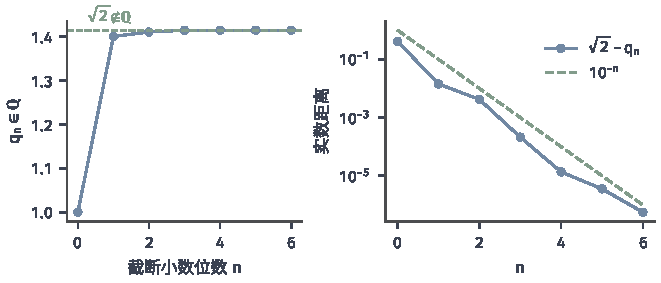
\includegraphics[width=112mm]{figures/01-mathematical-preliminaries-upper/01-mathematical-language-combinatorics-analysis-optimization/matplotlib/comprehension-additions/cauchy-completeness.pdf}
  \caption{令$q_n=\lfloor10^n\sqrt2\rfloor/10^n$，展示$n=0,\ldots,6$。左图各项均为有理数，虚线是实数极限$\sqrt2$；右图的实数距离满足$0<\sqrt2-q_n<10^{-n}$，用对数纵轴显示。有限个点不代替柯西性证明；该误差界与三角不等式才控制任意两个尾部项。}
  \label{fig:vol1-add-cauchy-completeness}
\end{figure}

\paragraph{闭集中的极限保留}

收敛与完备性保证逼近有终点后，还要检查终点是否仍满足原来的范围约束。前面用补集为开定义闭集，下面把这一条件改写为序列极限的保留条件。

\begin{lemma}[闭集的序列判据]
\label{lem:analysis-closed-sequence-criterion}
设$C$为度量空间$X$的子集。$C$闭当且仅当：对每个由$C$中点组成的序列，
若$x_n\to x$在$X$中成立，则$x\in C$。
\end{lemma}
\begin{proof}
若$C$闭而$x\notin C$，开集$X\setminus C$包含某个$B(x,r)$。
收敛要求充分靠后的$x_n$落入这个球，与$x_n\in C$矛盾。
反之，若$C$不闭，则存在$x\in X\setminus C$，使每个$B(x,r)$都与$C$相交。
为每个$n$选$x_n\in C\cap B(x,1/n)$，便有$x_n\to x\notin C$，违反序列条件。
\end{proof}

因此，完备度量空间的闭子集在继承的距离下也完备：子集中的柯西列先在母空间收敛，
闭性再保证极限仍在子集中。反过来，任一完备子空间在母度量空间中都是闭的，
因为在母空间收敛的子空间点列必为柯西列，子空间内的极限由唯一性等于原极限。
闭与有界描述不同性质；例如$(0,1)$有界但不闭，$\mathbb R$闭但不有界。

\subsection{输入趋近时的输出控制}
\label{sec:analysis-metric-continuity-extrema}

有了输入和输出的距离，就可以检查函数是否把接近的输入映成接近的输出。先在一个位置给出极限和连续性，再看能否为所有位置使用同一个输入精度。后两种统一控制分别由一致连续和Lipschitz条件表达。

\subsubsection{一点附近的函数变化}

\paragraph{函数极限与连续性}

对$f:X\to Y$及定义域$X$的一个聚点$a$（每个去掉$a$的邻域都含有$X$中的点），函数极限$\lim_{x\to a}f(x)=b$要求：对任意$\varepsilon>0$，存在$\delta>0$，使
\[
 0<d_X(x,a)<\delta\quad\Longrightarrow\quad d_Y(f(x),b)<\varepsilon.
\]
这里排除$x=a$，所以函数在$a$的取值甚至可以没有定义。连续性则要求$a$属于定义域，并把极限值与$f(a)$联系起来。对于定义域中的孤立点，足够小的邻域只含该点，连续性条件也自然成立。

确定输入与输出的距离后，可以要求小的输入扰动只引起小的输出扰动。这就把熟悉的
实函数连续性推广到一般度量空间。

为什么需要这项性质？因为它保证“先取极限再代入函数”与“先代入函数再取极限”结果相同。
若已知$x_n\to x$，我们希望$f(x_n)$的极限可以直接写成$f(x)$，而不必每换一列输入就
重做一次极限计算。连续映射就是允许这样做的函数；后面的隐函数定理、积分号下求导
都依赖这条替换规则。
\Needspace{12\baselineskip}
\begin{definition}[度量空间中的连续映射]
\label{def:analysis-continuity}
设$(X,d_X)$与$(Y,d_Y)$为度量空间。函数$f:X\to Y$在$x\in X$处
\term{连续}（continuous），是指
\[
  \begin{gathered}
    \forall\varepsilon>0,\quad \exists\delta>0,\quad \forall x'\in X,\\
    d_X(x,x')<\delta\Longrightarrow d_Y\bigl(f(x),f(x')\bigr)<\varepsilon.
  \end{gathered}
\]
若$f$在每个$x\in X$处连续，则称$f$在$X$上连续。
\end{definition}
这里$\delta$可以依赖所考察的位置$x$和要求的精度$\varepsilon$。在度量空间中，也可以用序列检验同一个条件：任意趋向$x$的$x_n$都使$f(x_n)$趋向$f(x)$。因此，已知$x_n\to x$且$f$在$x$处连续时，才可写成$f(\lim_nx_n)=\lim_nf(x_n)$；两端的趋近分别使用输入和输出空间的度量。

例如恒等映射$F(x)=x$从$(\mathbb R,d_1)$映到$(\mathbb R,d_2)$时处处不连续。
在任意$x$附近，总能找到通常距离任意小但不等于$x$的$x'$，它们的输出距离却始终为
$1$，无法小于$\varepsilon=1/2$。反过来，从$(\mathbb R,d_2)$到
$(\mathbb R,d_1)$的同一公式连续：选$\delta=1/2$，输入距离小于$\delta$就只可能
有$x'=x$，输出距离于是为$0$。这不是函数公式发生变化，而是输入输出空间对
“附近”的判断不同。图~\ref{fig:analysis-metric-convergence}右侧显示前一种失败。

\begin{figure*}[htbp]
  \centering
  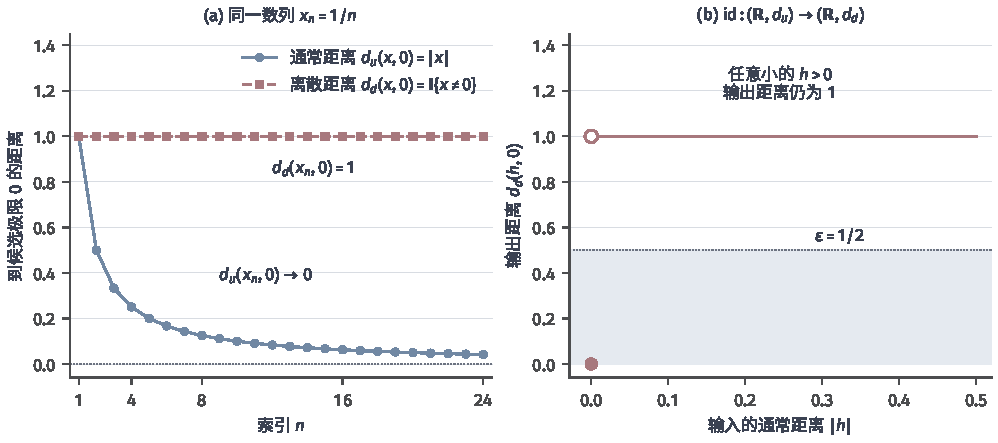
\includegraphics[width=169.0mm]{figures/01-mathematical-preliminaries-upper/01-mathematical-language-combinatorics-analysis-optimization/matplotlib/analysis-metric-convergence/figure.pdf}
  \caption{数值相同，距离不同。图中$d_u,d_d$分别对应正文的通常距离$d_1$与离散距离$d_2$。（a）数列 $x_n=1/n$ 到 $0$ 的通常距离趋于零，离散距离却恒为 $1$，所以收敛要连同度量说明。（b）恒等映射从通常度量空间映入离散度量空间时，任意非零且很小的输入位移仍对应输出距离 $1$，不能进入 $\varepsilon=1/2$ 的输出邻域，故它在 $0$ 处不连续。图为解析教学示例。}
  \label{fig:analysis-metric-convergence}
\end{figure*}

\paragraph{连续运算与函数复合}

连续性可以沿已有的计算关系传递。若$f,g:X\to\mathbb R$在$a$处连续，和、积都在$a$处连续；商还要求$g(a)\neq0$，连续性随后保证分母在一个邻域内不为零。若$f:X\to Y$在$a$处连续，$G:Y\to Z$在$f(a)$处连续，则$G\circ f$在$a$处连续。给定输出误差，先从$G$取得中间量的误差阈值，再从$f$取得输入阈值，就得到复合映射的控制。

这些规则建立在同一个位置的极限之上，不能跨过定义域限制。例如$1/x$在每个非零位置连续，却不能据此为$0$指定一个连续延拓；$|x|$处处连续，也仍需另查原点处是否存在共同斜率。

\subsubsection{整个范围上的变化控制}

\paragraph{一致连续的共同误差半径}

一个直观的图像是：普通连续只要求每个点周围都有一小片区域映射得足够近，但这片区域在陡峭处
可以缩得极小；一致连续则要求存在一个统一大小的“近邻半径”，在定义域任何位置都管用。
若要在事先不知道具体位置的情况下选一个输入误差阈值，并用它统一控制整个定义域的输出
误差，就需要让$\delta$不依赖位置。这一更强要求称为一致连续；它使同一个输入精度
足以控制整个定义域上的输出误差，因此可用于后面某些统一近似的证明。
它与函数列的一致收敛约束的对象不同：前者比较同一个函数在两个位置的值，后者比较
近似函数与目标函数在同一位置的值，不要求这些函数先一致连续。
\begin{definition}[一致连续映射]
\label{def:analysis-uniform-continuity}
设$(X,d_X)$与$(Y,d_Y)$为度量空间，$f:X\to Y$。若对每个$\varepsilon>0$都能找到一个与具体位置无关的$\delta>0$，使任意
$x,x'\in X$只要$d_X(x,x')<\delta$便有
$d_Y(f(x),f(x'))<\varepsilon$，就称$f$\term{一致连续}
（uniformly continuous）。
\end{definition}
连续性本身并不足以给出这种统一控制：
$f(x)=x^2$在$\mathbb{R}$上连续，令$x\to+\infty$并取$x'=x+1/x$，可见输入距离趋于零而输出距离
$|f(x')-f(x)|=2+1/x^2$不趋于零。

\paragraph{Lipschitz条件的比例控制}

一致连续给出统一的输入阈值，却没有要求输出误差与输入误差成固定比例。若还希望用一个常数直接估计误差的放大倍数，就要进一步要求线性上界。
\begin{definition}[Lipschitz连续映射]
\label{def:analysis-lipschitz-continuity}
设$(X,d_X)$与$(Y,d_Y)$为度量空间，$f:X\to Y$。若存在有限常数$L\geq0$，使所有$x,x'\in X$都满足
\begin{equation}
  d_Y\bigl(f(x),f(x')\bigr)\leq Ld_X(x,x'),
\label{eq:analysis-lipschitz-condition}
\end{equation}
则称$f$为$L$-\term{Lipschitz连续}（Lipschitz continuous）。
\end{definition}
当$L>0$时，取$\delta=\varepsilon/L$便得到一致连续性；$L=0$时函数为常值，也一致连续。
函数$f(x)=\sqrt{x}$在$[0,1]$上满足$|\sqrt{x}-\sqrt{x'}|\leq\sqrt{|x-x'|}$，
因而选$\delta=\varepsilon^2$就得到一致连续性，却不能得到Lipschitz连续性：若存在有限$L$，
令$x'=0$便会要求$\sqrt{x}\leq Lx$，即$1/\sqrt{x}\leq L$，这在$x\downarrow0$时不可能成立。
同一个公式在不同定义域上可能具有不同的统一控制。$f(x)=x^2$在$[0,1]$上满足
$|x^2-z^2|\leq2|x-z|$，因而$2$-Lipschitz；在整个实线上却没有有限的全局Lipschitz
常数。这两个例子说明，统一的$\varepsilon$--$\delta$控制与线性误差上界仍是不同要求。

\term{局部Lipschitz函数}（locally Lipschitz function）要求每个点附近的函数变化
都能由某个有限Lipschitz常数控制。与全局Lipschitz条件不同，各个邻域可以使用不同的常数。
\begin{definition}[局部Lipschitz函数]
\label{def:analysis-local-lipschitz}
设$U\subseteq\mathbb{R}^d$为开集，$f:U\to\mathbb{R}$。若对每个$\bm{x}\in U$，
都存在半径$r>0$与有限常数$L\geq0$，使$B(\bm{x},r)\subseteq U$，并且
\[
  |f(\bm{y})-f(\bm{z})|
  \leq L\lVert\bm{y}-\bm{z}\rVert_2
  \quad\text{对所有 }\bm{y},\bm{z}\in B(\bm{x},r)\text{成立},
\]
则称$f$在$U$上局部Lipschitz。
\end{definition}

这里$r$与$L$可以依赖中心点；一旦邻域确定，同一个$L$须控制其中的任意两点。
例如$f(x)=x^2$在任意$(x_0-r,x_0+r)$上可取$L=2(|x_0|+r)$，所以在实轴上
局部Lipschitz，却不是全局Lipschitz。向量值函数也用输出范数替换绝对值，
作完全相同的局部定义。局部控制要提升为区域内的统一控制，还需要区域或导数的额外条件。

\subsection{定义域限制下的统一控制与极值达到}

前面只规定函数的变化条件。现在把定义域也纳入判断：近似最优点可能逃向无穷远，或趋向被排除的边界。紧致性用于从序列中保留域内的极限子列；再与连续性结合，才得到极值达到和共同的误差尺度。

\subsubsection{有界序列能否保留收敛子列}

\paragraph{紧致性与有限覆盖}

第~\ref{chap:sets-functions-and-proofs}章已区分下确界与最小值：数值可以逼近一个下界，却始终找不到达到它的点。
要让近似最优点最终提供一个可行解，需要防止点列逃向无穷远或被排除的边界。
在一般度量空间中，承担这一职责的是紧致性。可以用一个最优化的直觉理解它：要在一列越来越好
的候选里取出真正的极限点，定义域必须是“封闭且走不出去”的，否则逼近序列可能收敛到定义域
边界外的点，那个点又恰好是最优值所在。紧致性正是这种“任何逼近序列都在域内留下聚点”的
保证。它并不保证函数有下界，只保证定义域本身
不留“逼近点可以逃出去”的缺口；配合连续性才能把下确界转成最小值。
\begin{definition}[开覆盖与紧致性]
\label{def:analysis-compactness}
设$(X,d)$为度量空间，$K\subseteq X$。若一族$X$中的开集的并包含$K$，就称这族开集为$K$的
\term{开覆盖}（open cover）；若从中选出的有限个开集仍覆盖$K$，它们就构成
\term{有限子覆盖}（finite subcover）。集合$K$的每个开覆盖都能选出有限子覆盖时，
称$K$为\term{紧致}（compact）。
\end{definition}
在度量空间中，这一定义等价于
\term{序列紧致性}：集合中的每个序列都有一个子序列收敛到仍在该集合中的点。
后一种表述更适合分析算法产生的点列，因为它直接提供候选极限。
我们先看开覆盖条件怎样保证这样的子列。若某个点列没有收敛子列，则对每个$x\in K$，
必有一个开球只含点列的有限项；否则可从$B(x,1/k)$中依次选取下标递增的项，构成趋于$x$的子列。
这些开球覆盖$K$，紧致性让我们选出有限个球覆盖$K$，于是整条点列也只能有有限项，矛盾。
这说明了当前需要的“开覆盖紧致$\Rightarrow$序列紧致”方向；反向等价在此不展开证明。

\paragraph{有限维中的闭且有界}

在有限维欧氏空间$\mathbb{R}^d$中，Heine--Borel定理说明紧致等价于闭且有界。这个结论不能原样搬到一般度量空间。考虑所有有界实数序列组成的空间
\[   \ell^\infty   =   \left\{\bm{x}=(x_1,x_2,\ldots):   \sup_{k\geq1}|x_k|<\infty\right\},   \qquad   d(\bm{x},\bm{y})=\sup_{k\geq1}|x_k-y_k|. \]
令$\bm{e}_n$只有第$n$个坐标为$1$，其余坐标为$0$。集合$\{\bm{e}_n:n\geq1\}$有界，且不同元素的距离恒为$1$。因此由该集合中元素组成的收敛点列必最终常值：柯西条件取误差$1/2$后，尾部不能再含两个不同元素。极限仍在集合内，由闭集的序列判据可知它闭。然而原点列$(\bm e_n)$的任何子序列都不是柯西数列，更不可能收敛。一般空间中 “闭且有界”不足以替代紧致，正是因为无穷多个彼此分离的方向可能留在同一个有界球内。

\subsubsection{连续函数能否达到极值}

\paragraph{极值达到的条件}

定义域能保留极限子列，还需让函数值随这些点连续变化，才能把近似极值变成实际达到的值。紧致性与连续性在下面分别承担这两项职责。

\begin{theorem}[紧致集上的极值定理]
\label{thm:analysis-extreme-value}
设$K$是非空紧致度量空间，$f:K\to\mathbb{R}$连续，则$f$在$K$上同时达到最小值与最大值。
\end{theorem}
这里回顾熟悉的极值定理，不再展开证明。紧致性的两项作用是从近似最优点列中抽出收敛子序列，并保证极限仍在可行集合内。连续性随后把函数值极限传到该点。任一条件缺失都可能使最优解不存在。
\begin{example}[极值存在条件怎样失效]
\label{ex:analysis-extrema-failures}
在开区间$(0,1)$上，连续函数$f(x)=x$的下确界为$0$，却没有最小点；定义域不紧致， 极限点$0$被排除。把定义域改成闭但不紧致的$\mathbb{R}$，连续函数$f(x)=e^x$仍有下确界$0$而不达到它。另一方面，在紧致集合$[0,1]$上定义
\[   g(0)=1,\qquad g(x)=x\quad(x>0), \]
则$\inf g=0$也未达到；这次失败的是$g$在$0$处不连续。三个例子分别表明“连续”、 “闭”或“有界”中的单独一项都不是一般的极值存在保证。
\end{example}

连续性控制函数值，不直接控制斜率。对一元函数，导数还要求左右两侧的差商趋向同一个值：$x^2$在$0$同时满足这两项要求，$|x|$的函数值趋向$0$却有两个不同的侧向斜率，阈值函数$\mathbb I\{x\geq0\}$则连左右函数值都不趋向同一个数。
尖点只阻止共同斜率，跳跃连共同的函数值极限也破坏了。
图~\ref{fig:analysis-continuity-counterexamples}把三者放在同一位置比较；
下一小节将写出差商和整体线性近似的正式条件。

\begin{figure*}[htbp]
  \centering
  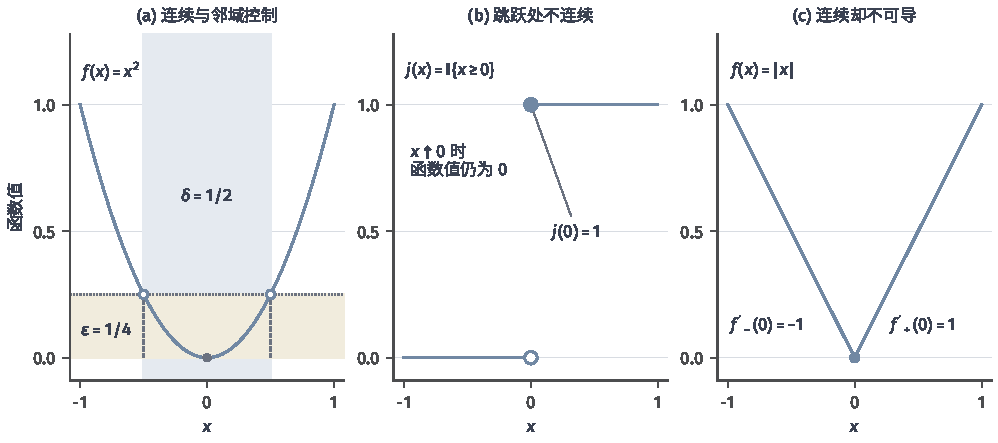
\includegraphics[width=169.0mm]{figures/01-mathematical-preliminaries-upper/01-mathematical-language-combinatorics-analysis-optimization/matplotlib/analysis-continuity-counterexamples/figure.pdf}
  \caption{三个不同的局部性质。（a）$f(x)=x^2$ 在 $0$ 处可用 $\delta=1/2$ 控制 $\varepsilon=1/4$：严格位于输入邻域内的点，其函数值严格落在输出邻域内。（b）阶跃函数在 $0$ 的左极限为 $0$，取值却为 $1$，空心点和实心点区分两者。（c）$|x|$ 在 $0$ 处连续，但左右导数分别为 $-1$ 和 $1$，不存在共同的双侧导数。图中曲线均为解析教学示例。}
  \label{fig:analysis-continuity-counterexamples}
\end{figure*}

\paragraph{紧致范围上的一致连续}

紧致性还能把逐点连续提升为一致连续：连续映射在紧致定义域上一定一致连续。
若它不一致连续，就能找到某个$\varepsilon_0>0$及点对$x_n,y_n\in K$，使
$d(x_n,y_n)<1/n$，而$d_Y(f(x_n),f(y_n))\geq\varepsilon_0$。
由序列紧致性选出$x_{n_k}\to x\in K$，三角不等式又给出$y_{n_k}\to x$。
连续性使两列函数值都趋于$f(x)$，与输出距离下界矛盾。
这为前面闭区间上的统一控制提供了一个一般条件，但不保证Lipschitz连续；
$\sqrt{x}$的例子已说明，输出变化未必能由输入距离的一次常数倍控制。

\section{函数的微分与局部近似}
\label{sec:analysis-local-models}

连续性保证输入变化足够小时输出变化也小，但没有说明变化沿什么方向、按什么比例发生。微分用局部线性或高阶模型回答这些问题。下面先建立变化的表示，再研究变化怎样沿复合计算、矩阵运算和隐式方程传递，最后控制有限位移与截断误差。尖点处的失效用方向差商说明，正式广义梯度放到第~\ref{chap:measurable-functions}章。

\subsection{局部变化的表示}
\label{sec:analysis-derivatives-linear-approximation}

在$f(x)=x^2$中，一个小输入增量可以分成线性响应和更小的余项；多元函数则要求所有小扰动共享一个线性响应。由此建立导数、全微分和Jacobian，再用Hessian描述线性响应怎样改变。对于绝对值的尖点，共同线性响应不存在，需要保留方向信息。

\subsubsection{一阶变化的线性表示}

\paragraph{差商、方向导数与偏导数}

从一元函数开始，把输出增量除以输入增量，得到这一小段上的平均变化率；
输入增量趋零后若仍有稳定值，就用它预测附近的输出。只保留一段的话，平均变化率会随
所取区间改变；使这个比值在区间长度趋零时有唯一极限，就把“局部斜率”从一个区间上的
平均值变成该点自身的性质。

一元函数$f:\mathbb{R}\to\mathbb{R}$在$x$处的\term{导数}（derivative）定义为
\[   f'(x)=\lim_{h\to0}\frac{f(x+h)-f(x)}{h}, \]
前提是这个双侧极限存在。
用一个具体数字体会它预测什么。取$f(x)=x^2$、$x=3$，在$h=0.1$时真实增量是
$3.1^2-3^2=0.61$，而用该点斜率$6$预测的一阶增量是$6\times0.1=0.6$，误差仅$0.01$；
$h$越小，这个相对误差越小。导数正是把“这一小段平均每单位输入变化引起多少输出变化”
在段长趋于零时的稳定值提取出来。
它说明输入发生小变化$h$时，函数增量的一阶部分是$f'(x)h$：
\begin{equation}
  f(x+h)=f(x)+f'(x)h+o(|h|).
\label{eq:analysis-scalar-first-order}
\end{equation}
第~\ref{sec:comb-growth-scales}节的小$o$仍表示相对余项趋零，不过这里的趋向是$h\to0$：余项$r(h)$满足$r(h)/|h|\to0$，不只是$h$本身很小。导数存在必然推出函数在该点连续，但连续不保证可导，例如$|x|$在$0$处连续，左右导数却分别为 $-1$和$1$。
这也解释了图中尖点与跳跃的区别；两者都不能使用经典双侧导数，失效的层次却不同。

对$f:\mathbb{R}^d\to\mathbb{R}$，沿方向$\bm{v}\in\mathbb{R}^d$的
\term{方向导数}（directional derivative）是
\[   D_{\bm{v}}f(\bm{x})   =   \lim_{t\to0}   \frac{f(\bm{x}+t\bm{v})-f(\bm{x})}{t}. \]
取$\bm{v}$为第$j$个坐标方向$\bm{e}_j$，就得到\term{偏导数}
（partial derivative）$\partial f/\partial x_j$。方向导数只检查一条直线，而整体可微性要求所有小扰动共享同一个线性近似。

\paragraph{全微分与Jacobian}

所有方向共享的近似还必须与扰动的叠加和缩放相容：把扰动写成
$\alpha\bm u+\beta\bm v$时，预测增量也应为两部分预测增量的同样组合。
满足
\[
 A(\alpha\bm u+\beta\bm v)=\alpha A(\bm u)+\beta A(\bm v)
 \quad(\bm u,\bm v\in\mathbb R^d,\ \alpha,\beta\in\mathbb R)
\]
的映射称为线性映射。例如固定向量$\bm a$后，$A(\bm h)=\bm a^\top\bm h$
把每个坐标的扰动乘以固定系数再相加。可微性要求用同一个这样的映射解释全部小扰动。

函数$f:\mathbb{R}^d\to\mathbb{R}$在$\bm{x}$处\term{可微}
（differentiable），是指存在一个线性映射 $A:\mathbb{R}^d\to\mathbb{R}$，使
\begin{equation}
  f(\bm{x}+\bm{h})
  =
  f(\bm{x})+A(\bm{h})+o(\lVert\bm{h}\rVert_2).
\label{eq:analysis-total-differentiability}
\end{equation}
线性部分$A(\bm h)$称为全微分，也记为$\mathrm df_{\bm x}(\bm h)$。
条件要求对任意趋零的非零扰动$\bm h$都有
$|f(\bm x+\bm h)-f(\bm x)-A(\bm h)|/\lVert\bm h\rVert_2\to0$，
而不是先固定一个方向，再允许误差控制随方向改变。
在欧氏空间中，每个这样的线性泛函都可写为 $A(\bm{h})=\langle\nabla f(\bm{x}),\bm{h}\rangle$，其中
\[   \nabla f(\bm{x})   =   \left(     \frac{\partial f}{\partial x_1}(\bm{x}),\ldots,     \frac{\partial f}{\partial x_d}(\bm{x})   \right)^{\top} \]
称为\term{梯度}（gradient）。因此梯度不是若干偏导数的随意排列，而是表示局部线性映射的向量；扰动$\bm{h}$通过内积变成函数的一阶变化。

可微必然推出所有方向导数存在，并且 $D_{\bm{v}}f(\bm{x})=\langle\nabla f(\bm{x}),\bm{v}\rangle$。反向结论不成立， 仅有偏导数更不够。
\begin{example}[偏导数存在但不可微]
\label{ex:analysis-partials-not-differentiable}
定义$f:\mathbb{R}^2\to\mathbb{R}$为
\[   f(x,y)=
\begin{cases}     \dfrac{xy}{\sqrt{x^2+y^2}}, & (x,y)\neq(0,0),\\[6pt]     0, & (x,y)=(0,0).
\end{cases} \]
沿两条坐标轴，函数恒为$0$，所以 $\partial f/\partial x(0,0)=\partial f/\partial y(0,0)=0$。若$f$在原点可微， 候选线性部分只能是零映射。可是沿$\bm{h}=(t,t)$，
\[   \frac{|f(t,t)-f(0,0)|}{\lVert(t,t)\rVert_2}   =   \frac{|t|/\sqrt{2}}{\sqrt{2}|t|}   =\frac12, \]
余项与$\lVert\bm{h}\rVert_2$之比不趋于零，故$f$在原点不可微。偏导数只看坐标轴，遗漏了其他接近路径。本例沿每个方向$\bm v=(a,b)$的
正向方向导数都存在，这里只令$t\downarrow0$，得到$ab/\sqrt{a^2+b^2}$（零方向取$0$）；它却不是关于$\bm v$
的线性函数，而且双侧方向导数在$ab\neq0$时不存在。方向极限采用单侧还是双侧，
必须与所用定义一致；本节定义采用双侧极限。
\end{example}

一个常用的充分条件是：若$f$的所有一阶偏导数在$\bm{x}$的某个邻域内存在，并在 $\bm{x}$处连续，则$f$在$\bm{x}$处可微。注意这只是方便核对的充分条件，不是必要条件； 可微函数的偏导数不一定在该点附近连续。

即使每个双侧方向导数都存在，也未必可微。例如令
$g(x,y)=x^3/(x^2+y^2)$于非零点，$g(0,0)=0$。
沿$\bm v=(a,b)\neq\bm0$有$D_{\bm v}g(0,0)=a^3/(a^2+b^2)$，
但坐标方向导数给出的候选梯度为$(1,0)^\top$，它对方向$(1,1)^\top$
预测$1$而非实际的$1/2$。这些方向变化率无法拼成一个线性映射。
与前例的单侧方向极限相比，这里直接检验了本节采用的双侧定义。

用$f(x)=x^3-3x$保留一个贯穿例子。在$x_0=1/2$处，
\[
  f(x_0)=-\frac{11}{8},\qquad f'(x_0)=3x_0^2-3=-\frac94.
\]
输入改变$h$时，一阶近似给出
\begin{equation}
  T_1(h)=f(x_0)+f'(x_0)h=-\frac{11}{8}-\frac94h.
\label{eq:analysis-cubic-linear-model}
\end{equation}
取$h=0.1$，$T_1(h)=-1.600$，而实际$f(0.6)=-1.584$。近似抓住了下降方向和主要
变化量，但还有$0.016$的误差；第~\ref{sec:analysis-second-order-curvature}节将用曲率解释这部分差别。

当一个输入产生多个输出时，每个输出都有一行局部线性系数，把这些行排在一起便得到
Jacobian矩阵。复合计算只需再把前一层的输出扰动作为后一层的输入扰动。
设$f:\mathbb{R}^d\to\mathbb{R}^m$。若存在矩阵 $\bm{J}_f(\bm{x})\in\mathbb{R}^{m\times d}$使
\begin{equation}
  f(\bm{x}+\bm{h})
  =
  f(\bm{x})+\bm{J}_f(\bm{x})\bm{h}
  +o(\lVert\bm{h}\rVert_2),
\label{eq:analysis-jacobian-linearization}
\end{equation}
则称$f$在$\bm{x}$处可微，$\bm{J}_f(\bm{x})$称为
\term{Jacobian矩阵}（Jacobian matrix）。其第$i,j$个元素是 $\partial f_i/\partial x_j$。矩阵有$m$行、$d$列，因为它把$d$维输入扰动映射成 $m$维输出扰动。

\subsubsection{二阶变化的曲率表示}
\label{sec:analysis-second-order-curvature}

\paragraph{Hessian与方向曲率}

上一节的线性近似在$x_0=1/2$处把函数值预测为$-1.600$，实际为$-1.584$，偏差$0.016$。
这个偏差从哪里来？因为斜率本身也在随位置改变。要估计这个偏差，就要知道斜率沿每个方向
改变得多快，这需要比一阶导数更高一阶的信息。

延续$f(x)=x^3-3x$的例子，一阶导数$f'(x)=3x^2-3$还随位置变化。再求一次导数，
得到$f''(x)=6x$，所以$f''(1/2)=3$。在$x_0=1/2$附近，斜率向右移动时增大，
曲线向上弯；这解释了真实值为何高于前节的切线预测。图~\ref{fig:analysis-derivative-orders}将切线和下面的二次修正放在同一幅曲线图上比较。加入二次项得到
\begin{equation}
  T_2(h)=T_1(h)+\frac12f''(x_0)h^2
        =-\frac{11}{8}-\frac94h+\frac32h^2.
\label{eq:analysis-cubic-quadratic-model}
\end{equation}
在$h=0.1$时，$T_2=-1.585$，与实际值$-1.584$只差$0.001$。
一阶导数回答此处沿给定方向增还是减，二阶导数回答这个变化率怎样改变。
第~\ref{sec:analysis-taylor-approximation}节将用Taylor展开给出一阶和二阶余项的完整表达式。

一阶近似只保留函数的局部斜率。若还要判断这个斜率怎样随位置改变，就需要
\term{Hessian矩阵}（Hessian matrix）。设$f:\mathbb{R}^d\to\mathbb{R}$在 $\bm{x}$附近二阶可微，定义
\[   \nabla^2 f(\bm{x})   =
\begin{bmatrix}     \dfrac{\partial^2 f}{\partial x_1^2} &     \cdots &     \dfrac{\partial^2 f}{\partial x_1\partial x_d}\\     \vdots & \ddots & \vdots\\     \dfrac{\partial^2 f}{\partial x_d\partial x_1} &     \cdots &     \dfrac{\partial^2 f}{\partial x_d^2}
\end{bmatrix}. \]
若二阶偏导数在邻域内连续，混合偏导数可以交换，Hessian矩阵因而对称。
这里把方表$\bm H$与方向$\bm v$组合而成的二次表达式
$\bm v^\top\bm H\bm v=\sum_{i=1}^d\sum_{j=1}^d H_{i,j}v_i v_j$称为二次型。
对方向$\bm v$，$\bm{v}^{\top}\nabla^2f(\bm{x})\bm{v}$是沿直线
$t\mapsto f(\bm{x}+t\bm{v})$在$t=0$处的二阶导数。它衡量的是沿该方向的一阶斜率变化。

对二次函数
\[   f(\bm{x})   =   \frac12\bm{x}^{\top}\bm{A}\bm{x}   +\bm{b}^{\top}\bm{x}+c, \]
只有$\bm{A}$的对称部分影响函数值。令 $\bm{H}=(\bm{A}+\bm{A}^{\top})/2$，则 $\nabla f(\bm{x})=\bm{H}\bm{x}+\bm{b}$且 $\nabla^2f(\bm{x})=\bm{H}$。
例如$\bm H=\operatorname{diag}(2,100)$时，方向二次型为$2v_1^2+100v_2^2$，
沿两个坐标方向都向上弯，但第二个方向的二阶变化率是第一个的$50$倍。
若改为$\operatorname{diag}(2,-100)$，两个坐标方向的弯曲方向便相反。
判断曲率需要检查整个二次型，而不是某一个对角元素。

对实对称矩阵$\bm H$，若每个非零$\bm v$都有$\bm v^\top\bm H\bm v>0$，称$\bm H$正定；
若只要求$\bm v^\top\bm H\bm v\geq0$，则称半正定。
把不等号反向得到负定与半负定；若既存在使二次型为正的方向，又存在使它为负的方向，
则称矩阵不定。这些名称分别说明全部方向或某些方向上的曲率符号。

\paragraph{驻点附近的局部形状}

函数在当前点附近是增是减，可用于判断局部极值。局部极小点是指某个邻域内
所有函数值都不小于该点的值；严格局部极小还要求其他点的值严格更大。
设$\bm{x}^{\star}$是开集内部的局部极小点，且$f$在该点可微。对每个方向 $\bm{v}$考察$f(\bm{x}^{\star}+t\bm{v})$，一元函数的必要条件给出 $\nabla f(\bm{x}^{\star})^{\top}\bm{v}=0$。这对所有$\bm{v}$成立，因此
\begin{equation}
  \nabla f(\bm{x}^{\star})=\bm{0}.
\label{eq:analysis-first-order-necessary}
\end{equation}
若$f$还在该点二阶可微，同样沿任意方向使用一元二阶必要条件，可得
\begin{equation}
  \bm{v}^{\top}\nabla^2f(\bm{x}^{\star})\bm{v}\geq0
  \quad\text{对所有 }\bm{v},
\label{eq:analysis-second-order-necessary}
\end{equation}
即Hessian矩阵半正定。局部极大点对应半负定。这些只是必要条件：
$f(x)=x^4$与$f(x)=-x^4$在$0$处分别有严格局部极小值和严格局部极大值，
二者的二阶导数却都为零；$f(x)=x^3$在$0$处的一阶导数和二阶导数也都为零，
却没有极值。Hessian矩阵半正定或半负定本身不能决定驻点类型。

驻点处各方向的二阶变化都为正，即Hessian正定，并且函数在邻域内二阶连续可微时，该点是严格局部极小点；负定时对应严格局部极大点。不定时存在一增一减两个方向，形成鞍点。这里只先说明判别的含义；从局部曲率到原函数的严格判断，还需要控制高阶余项，第~\ref{sec:analysis-taylor-approximation}节将给出完整论证。

\subsubsection{不可微位置的方向变化}
\label{sec:analysis-directional-nonsmooth}

\paragraph{尖点处的单边变化}

绝对值在$0$处连续，右侧差商为$1$，左侧差商为$-1$，因此没有共同的双侧导数。若只考察从当前位置沿给定方向前进，可以令$t\downarrow0$，定义正向方向差商的极限
\[
 D^+_v f(x)=\lim_{t\downarrow0}\frac{f(x+tv)-f(x)}{t}.
\]
对$f(x)=|x|$及$x=0$，这个极限为$|v|$。它对每个方向都有值，却不满足线性性：方向$1$和$-1$都得到$1$。ReLU函数$\max\{0,x\}$在$0$处同样有正向方向导数$\max\{0,v\}$。这里采用的正向极限与前面双侧方向导数是两个约定，使用时必须写明。

\paragraph{方向信息与单一梯度的边界}

如果一个向量真能表示全微分，其与方向的内积必须同时给出所有方向的一阶变化。绝对值和ReLU的正向方向变化不满足这一要求，任意指定一个梯度值也不能使函数变得可微。第~\ref{chap:measurable-functions}章将在局部Lipschitz条件下，用附近可微位置的梯度集合描述尖点；这仍不等于在尖点恢复一个经典导数。


在含阈值或脉冲事件的模型中，常保留离散前向映射，却在反向计算时把其导数替换成某个平滑且非零的函数。这种信号称为\term{替代梯度}（surrogate gradient）。它是算法人为指定的近似更新方向，不自动等于前向映射的经典导数，也通常不满足凸次梯度的不等式。因此使用时应分别写清前向函数、反向替代函数及其尺度，不能把训练规则描述成对原离散函数的精确求导。

中心差分
\[   \frac{f(x+\varepsilon)-f(x-\varepsilon)}{2\varepsilon} \]
检验的是实际代入的函数$f$在尺度$\varepsilon$上的变化。若前向计算采用离散函数，反向计算另行指定平滑信号，差分与反向信号就对应不同对象。核验程序时，应分别检查离散前向函数是否正确，以及反向信号是否符合指定的学习规则；不能把二者相等作为未经说明的检验标准。

\subsection{函数关系中的变化传递}
\label{sec:analysis-vector-chain-matrix-calculus}

实际计算往往把多个函数连接起来，或由矩阵运算、方程关系间接决定输出。它们共享的任务是把已知的局部变化传到最终结果，但所需信息不同：复合映射直接传递Jacobian；矩阵变量要保持乘法结构；隐式关系还必须先保证存在可微解分支。

\subsubsection{复合映射中的变化传递}

\paragraph{链式法则与乘法顺序}

若一次计算的输出成为下一次计算的输入，前一映射产生的局部扰动还要再经过后一映射的线性响应。复合后的响应因此是两个Jacobian的乘积，先后次序由实际计算关系决定。

若$f$在$\bm{x}$处可微，且$g:\mathbb{R}^m\to\mathbb{R}^p$在$f(\bm{x})$处可微，则复合映射满足
\begin{equation}
  \bm{J}_{g\circ f}(\bm{x})
  =
  \bm{J}_g\bigl(f(\bm{x})\bigr)\bm{J}_f(\bm{x}).
\label{eq:analysis-vector-chain-rule}
\end{equation}
这就是\term{链式法则}（chain rule）。维度同时给出乘法次序： $(p\times m)(m\times d)=p\times d$，反向相乘往往没有定义。即使方阵$\bm A,\bm B$同阶、两个次序的乘积都有定义，也通常有$\bm A\bm B\neq\bm B\bm A$，不能据标量求导经验调换因子。

\paragraph{标量目标的反向求导}

上面的$g$允许向量输出。当$p=1$时，$g$把中间向量变成一个标量。在优化问题中，
这个标量通常是待最小化的目标值，本书便把此时的$g$记为$\ell$。令
$\bm y=f(\bm x)$，总目标就是$L(\bm x)=\ell(f(\bm x))$；$\ell$只是原复合映射的
最后一层，并没有增加一个未说明的输出。采用列向量梯度，链式法则写成
\[
  \nabla L(\bm x)
  =\bm J_f(\bm x)^\top\nabla\ell(\bm y)\big|_{\bm y=f(\bm x)}.
\]
局部线性映射在前向计算中按$\bm J_f$作用，在标量目标的反向计算中按转置
$\bm J_f^\top$传回。这是后续反向传播的线性代数核心，具体网络结构留到模型章节。

\begin{example}[从中间向量求回复合目标的梯度]
\label{ex:analysis-chain-rule-calculation}
令
\[
  f(x_1,x_2)=(x_1^2,x_1x_2,x_2)^\top,
  \qquad \ell(\bm y)=\frac12(y_1^2+y_2^2+y_3^2).
\]
$f$从二维输入产生三维中间量，$\ell$再把三维中间量变成一个数。于是
\[
  \bm J_f=\begin{bmatrix}2x_1&0\\x_2&x_1\\0&1\end{bmatrix},
  \qquad \nabla\ell(\bm y)=\bm y.
\]
在$\bm x=(1,2)^\top$处，$\bm y=(1,2,2)^\top$，链式法则给出
\[
  \nabla L(1,2)
  =\begin{bmatrix}2&2&0\\0&1&1\end{bmatrix}
    \begin{bmatrix}1\\2\\2\end{bmatrix}
  =\begin{bmatrix}6\\4\end{bmatrix}.
\]
也可以把复合函数直接展开为
$L(x_1,x_2)=\tfrac12(x_1^4+x_1^2x_2^2+x_2^2)$，求偏导得到
$\nabla L=(2x_1^3+x_1x_2^2,\,x_1^2x_2+x_2)^\top$，在同一点仍为$(6,4)^\top$。
两种计算处理同一个目标；链式形式保留了中间映射，可分别复用各层的导数。
矩阵形状$(2\times3)(3\times1)=2\times1$也核对了梯度传递的次序。
\end{example}

若要把任意实数评分变成正数且总和为$1$的权重，可以先取指数再除以共同的总和。
这就是$n$维\term{归一化指数映射}（softmax）。对正整数$n$和
$\bm{z}\in\mathbb{R}^n$，令
\[
  s_i(\bm{z})
  =
  \frac{e^{z_i}}{\sum_{k=1}^n e^{z_k}},
  \qquad i=1,\ldots,n.
\]
记分母为$Z=\sum_k e^{z_k}$。指数函数求导和商法则给出
\[
  \frac{\partial s_i}{\partial z_j}
  =
  \frac{\mathbb{I}\{i=j\}e^{z_i}Z-e^{z_i}e^{z_j}}{Z^2}
  =
  s_i\bigl(\mathbb{I}\{i=j\}-s_j\bigr).
\]
因此整个Jacobian矩阵为
\begin{equation}
  \bm{J}_{\bm{s}}(\bm{z})
  =
  \operatorname{diag}(\bm{s})-\bm{s}\bm{s}^{\top}.
\label{eq:analysis-softmax-jacobian}
\end{equation}
对角项$s_i(1-s_i)$描述提高$z_i$对自身分量的影响，非对角项$-s_is_j$
来自共同分母：提高一个坐标会压低其余归一化分量。每行元素之和为零，
这也与给所有$z_i$同时加同一常数不改变输出相符。

\subsubsection{矩阵运算中的变化传递}

\paragraph{矩阵微分与迹内积}

第~\ref{chap:sets-functions-and-proofs}章已经建立矩阵乘法和转置。以下还用到逆矩阵、迹与行列式：逆矩阵$\bm X^{-1}$满足$\bm X\bm X^{-1}=\bm X^{-1}\bm X=\bm I$；对$d$阶方阵，行列式是$\det\bm X=\sum_{\pi\in S_d}\operatorname{sgn}(\pi)\prod_iX_{i,\pi(i)}$，其中$S_d$为排列集合，符号由排列的奇偶性决定。它为零恰好表示矩阵不可逆。这里采用这些有限维代数事实，系统推导见第~\ref{chap:linear-algebra}章。后面的迹内积和乘积展开会直接说明所需微分，不要求提前掌握整章线性代数。

如果输入本身是矩阵，逐条写出$mn$个偏导数会掩盖原有的矩阵乘法结构。矩阵$\bm{X}\in\mathbb{R}^{m\times n}$可以看成$mn$个坐标组成的对象，矩阵梯度则把这些一阶变化重新排回原来的形状。先固定Frobenius迹内积
\[   \langle\bm{A},\bm{B}\rangle_F   =   \operatorname{tr}(\bm{A}^{\top}\bm{B}) \]
其中$\operatorname{tr}$是方阵对角元素之和，所以这个内积也等于
$\sum_{i,j}\bm A_{i,j}\bm B_{i,j}$，对应范数为
$\lVert\bm H\rVert_F=(\sum_{i,j}\bm H_{i,j}^2)^{1/2}$。
对标量函数$f(\bm X)$，全微分要求
$f(\bm X+\bm H)=f(\bm X)+\mathrm df_{\bm X}(\bm H)+o(\lVert\bm H\rVert_F)$。
用这个内积
定义矩阵梯度：若一阶全微分能够写成
\begin{equation}
  \mathrm{d}f
  =
  \langle\nabla_{\bm{X}}f,\mathrm{d}\bm{X}\rangle_F
  =
  \operatorname{tr}\bigl((\nabla_{\bm{X}}f)^{\top}
  \mathrm{d}\bm{X}\bigr),
\label{eq:analysis-matrix-gradient-definition}
\end{equation}
则$\nabla_{\bm{X}}f$与$\bm{X}$形状相同。计算时可先用乘积法则展开微分，再利用
\[   \operatorname{tr}(\bm{A}\bm{B})   =\operatorname{tr}(\bm{B}\bm{A}),\qquad   \operatorname{tr}(\bm{A}\bm{B}\bm{C})   =\operatorname{tr}(\bm{B}\bm{C}\bm{A}), \]
把$\mathrm{d}\bm{X}$移动到末端。迹只允许循环移位，不能任意交换相邻矩阵。

先考虑二次型$q(\bm{x})=\bm{x}^{\top}\bm{A}\bm{x}$，其中 $\bm{A}\in\mathbb{R}^{d\times d}$固定。由乘积法则，
\begin{align*}
  \mathrm{d}q
  &=
  (\mathrm{d}\bm{x})^{\top}\bm{A}\bm{x}
  +\bm{x}^{\top}\bm{A}\,\mathrm{d}\bm{x}\\
  &=
  \bm{x}^{\top}(\bm{A}^{\top}+\bm{A})\,\mathrm{d}\bm{x}.
\end{align*}
因此
\begin{equation}
  \nabla_{\bm{x}}
  \bigl(\bm{x}^{\top}\bm{A}\bm{x}\bigr)
  =
  (\bm{A}+\bm{A}^{\top})\bm{x}.
\label{eq:analysis-quadratic-form-gradient}
\end{equation}
只有当$\bm{A}$对称时才能化为$2\bm{A}\bm{x}$。直接写成$2\bm{A}\bm{x}$会悄然加入对称性条件。

对固定的$\bm{A}\in\mathbb{R}^{m\times n}$，令 $f(\bm{X})=\operatorname{tr}(\bm{A}^{\top}\bm{X})$。它的微分已经符合式
\eqref{eq:analysis-matrix-gradient-definition}，所以
\begin{equation}
  \nabla_{\bm{X}}\operatorname{tr}(\bm{A}^{\top}\bm{X})
  =\bm{A}.
\label{eq:analysis-trace-linear-gradient}
\end{equation}
这个简单关系常用于从迹表达式中读出梯度。

\paragraph{逆矩阵与行列式的变化}

若方阵$\bm{X}$可逆，由恒等式$\bm{X}\bm{X}^{-1}=\bm{I}$取微分可得
\[   (\mathrm{d}\bm{X})\bm{X}^{-1}   +\bm{X}\,\mathrm{d}(\bm{X}^{-1})=\bm{0}. \]
左乘$\bm{X}^{-1}$后得到
\begin{equation}
  \mathrm{d}(\bm{X}^{-1})
  =
  -\bm{X}^{-1}(\mathrm{d}\bm{X})\bm{X}^{-1}.
\label{eq:analysis-inverse-differential}
\end{equation}
两个$\bm{X}^{-1}$位于扰动两侧，不能合并成 $-\bm{X}^{-2}\mathrm{d}\bm{X}$，因为$\mathrm{d}\bm{X}$未必与$\bm{X}^{-1}$交换。

最后设$\bm{X}\in\mathbb{R}^{d\times d}$可逆且$\det\bm{X}>0$，使实值函数$\log\det\bm{X}$有定义。
计算它的一阶变化，先把方向扰动$\bm H$从行列式中分离出来：
\[
 \det(\bm X+t\bm H)=\det(\bm X)\det(\bm I+t\bm X^{-1}\bm H).
\]
对固定矩阵$\bm B$，行列式的排列展开给出
$\det(\bm I+t\bm B)=1+t\operatorname{tr}(\bm B)+O(t^2)$。
其中一次项只能从恒等排列的一个对角位置选取$tB_{i,i}$，其余位置选$1$；
非恒等排列至少改变两个位置，因此只贡献二次及以上项。
代入$\bm B=\bm X^{-1}\bm H$，便得到Jacobi行列式公式的一阶形式
\[   \mathrm{d}\det\bm{X}   =   \det(\bm{X})\operatorname{tr}   (\bm{X}^{-1}\mathrm{d}\bm{X}). \]
再应用标量对数的链式法则，
\begin{equation}
  \mathrm{d}\log\det\bm{X}
  =
  \operatorname{tr}(\bm{X}^{-1}\mathrm{d}\bm{X}),
  \qquad
  \nabla_{\bm{X}}\log\det\bm{X}
  =
  \bm{X}^{-\top}.
\label{eq:analysis-logdet-gradient}
\end{equation}
若$\bm X$还对称，则$\bm{X}^{-\top}=\bm{X}^{-1}$；一般情形应保留转置。
这些计算都先找出扰动的一阶项，再用迹内积读出梯度；乘积次序与行列式展开决定了哪些变形成立。
\begin{example}[逆矩阵微分中的乘法次序]
\label{ex:analysis-noncommuting-inverse-differential}
取$\bm X=\operatorname{diag}(2,1)$，扰动方向
$\bm E=\begin{bmatrix}0&1\\1&0\end{bmatrix}$。沿$\bm X+t\bm E$求逆矩阵的导数为
\[
 -\bm X^{-1}\bm E\bm X^{-1}
 =\begin{bmatrix}0&-1/2\\-1/2&0\end{bmatrix}.
\]
若照搬标量规则而写成$-\bm X^{-2}\bm E$，会得到
$\begin{bmatrix}0&-1/4\\-1&0\end{bmatrix}$，连对称性都丢失。
原路径在$0$附近由对称可逆矩阵组成，其逆与导数也应对称；这一结构检查能直接发现错误。
矩阵变量沿给定方向微分时，夹在两侧的逆矩阵不能随意移到同一侧。
\end{example}

\subsubsection{隐式方程中的变化传递}
\label{sec:analysis-implicit-parameter-integral}

\paragraph{局部解分支的存在条件}

显式函数给出了每个输入对应的输出，方程$F(\bm x,\bm y)=\bm0$却只规定两者必须满足的关系。
这类关系在优化里反复出现。把一组可变化的观测数值记为$\bm\theta$，参数为$\bm w$，
目标写成$J(\bm w,\bm\theta)$；驻点方程$\nabla_{\bm w}J(\bm w,\bm\theta)=\bm0$
规定了两者的关系，却没有直接给出$\bm w$关于$\bm\theta$的公式。
想知道观测数值微调后驻点怎样移动，需要先固定一个驻点，再确认方程在它附近确定
唯一且可微的分支。驻点还可能是极大点或鞍点，不能仅凭这个方程就称为最优参数；
若要追踪局部极小解，还需另行核验极小性条件，局部结论也不保证全局最优。
回到一般方程$F(\bm x,\bm y)=\bm0$，固定$\bm x$以后，可能有多个$\bm y$，也可能没有解。
讨论$\bm y$随$\bm x$的局部变化，需要先证明某个解附近存在唯一且可微的解分支。

需要这一步，是因为链式法则不能对“某条隐藏的依赖关系”使用。对方程两端求导时必须指明
正在对哪一个函数求导；若解不唯一，导数在同一个$\bm x$处对应不同的值，公式无从谈起。
下面的定理给出的是一组充分条件，使方程在一点附近确定唯一的可微解函数，并保证该函数
的导数由方程本身的偏导数算出。这样得到的解导数用于两件事：追踪解的移动，以及判断
最优值随参数怎样变化。这里先陈述局部存在与可微性的条件，再计算导数；压缩迭代的构造证明将放到第~\ref{sec:analysis-complete-contraction}节。驻点方程是应用这项结果的一个例子。

例如方程$y^2-x=0$在$x>0$时有正、负两支解。固定其中一个非零解后，可以在它附近选出唯一分支；但在$(0,0)$，两支相交，负$x$侧还没有实数解，因此不存在覆盖$0$的开区间上的可微解函数。此处$\partial F/\partial y=2y=0$，恰好失去了下面定理要求的可逆性。这个例子说明，局部选解既要指定起始解，也要核对关于待解变量的导数。


图~\ref{fig:vol1-add-implicit-branches}说明“局部唯一”怎样排除另一支解。在$(1,1)$附近只保留正支即可；在原点处，两支相交且负$x$没有实数解，不能沿用同样的局部可微选解。
\begin{figure}[!htb]
  \centering
  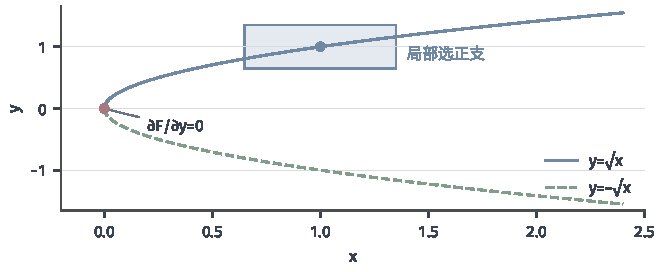
\includegraphics[width=112mm]{figures/01-mathematical-preliminaries-upper/01-mathematical-language-combinatorics-analysis-optimization/matplotlib/comprehension-additions/implicit-branches.pdf}
  \caption{方程$F(x,y)=y^2-x=0$的两支实数解。浅蓝矩形围住$(1,1)$，在该矩形内每个允许的$x$只有正支解，且$F_y=2y\neq0$；红点处$F_y=0$，两支相交。图的两个根都属于同一方程，选定起始解与邻域才确定隐函数分支。}
  \label{fig:vol1-add-implicit-branches}
\end{figure}

\begin{theorem}[隐函数定理]
\label{thm:analysis-implicit-function}
设$F:\mathbb{R}^p\times\mathbb{R}^m\to\mathbb{R}^m$在 $(\bm{a},\bm{b})$的某个开邻域内连续可微， $F(\bm{a},\bm{b})=\bm{0}$，并且关于待解变量的Jacobian矩阵 \[   \bm{D}_{\bm{y}}F(\bm{a},\bm{b})   \in\mathbb{R}^{m\times m} \]
可逆。则存在$\bm{a}$与$\bm{b}$的邻域$U,V$，以及唯一的连续可微函数
$\varphi:U\to V$，使$\varphi(\bm{a})=\bm{b}$，并且对所有
$(\bm{x},\bm{y})\in U\times V$都有
\[
  F(\bm{x},\bm{y})=\bm{0}
  \quad\Longleftrightarrow\quad
  \bm{y}=\varphi(\bm{x}).
\]
其Jacobian矩阵满足
\begin{equation}
  \bm{D}\varphi(\bm{x})
  =
  -
  \bigl[\bm{D}_{\bm{y}}F(\bm{x},\varphi(\bm{x}))\bigr]^{-1}
  \bm{D}_{\bm{x}}F(\bm{x},\varphi(\bm{x})).
\label{eq:analysis-implicit-derivative}
\end{equation}
\end{theorem}

\paragraph{解变化与代回目标后的变化}

定理的存在、局部唯一性和可微性不能由形式求导代替。这里先使用其陈述；第~\ref{sec:analysis-complete-contraction}节建立压缩迭代后，将补全构造证明。一旦确认$\varphi$可微，导数公式也可以直接由链式法则读出：对$F(\bm x,\varphi(\bm x))=\bm0$求导，得到
\[
 \bm D_{\bm x}F+\bm D_{\bm y}F\,\bm D\varphi=\bm0.
\]
左乘关于待解变量的Jacobian的逆，就得到式~\eqref{eq:analysis-implicit-derivative}。这个公式先给出解的移动；若把解代回另一个目标，还需再作一次复合求导。



考虑依赖参数$\theta$的无约束目标$q(z,\theta)$。若局部最优解$z^\star(\theta)$位于定义域内部，它满足驻点方程
\[   F(\theta,z)   =   \frac{\partial q}{\partial z}(z,\theta)   =   0. \]
若$q$二阶连续可微，且 $\partial^2q/\partial z^2$在所考察解处非零，隐函数定理给出该驻点的局部唯一分支。这并不自动说明它是全局最优解；还要由曲率或其他结构核对最优性。
\begin{example}[参数二次目标中的解导数与包络导数]
\label{ex:analysis-parametric-quadratic}
对$\theta>-1$，令
\[   q(z,\theta)   =   \frac12(1+\theta)z^2-\theta z. \]
因为$\theta>-1$，配方得到
\[
  q(z,\theta)=\frac{1+\theta}{2}
  \left(z-\frac{\theta}{1+\theta}\right)^2
  -\frac{\theta^2}{2(1+\theta)}.
\]
平方项的系数为正，所以唯一驻点就是全局最小点。驻点方程为
\[   F(\theta,z)=(1+\theta)z-\theta=0. \]
隐式求导给出
\[   \frac{\mathrm{d}z^\star}{\mathrm{d}\theta}   =   -\frac{\partial F/\partial\theta}{\partial F/\partial z}   =   -\frac{z^\star-1}{1+\theta}. \]
直接消元得到
\[   z^\star(\theta)=\frac{\theta}{1+\theta},   \qquad   \frac{\mathrm{d}z^\star}{\mathrm{d}\theta}   =   \frac{1}{(1+\theta)^2}, \]
两种计算一致。

最优值$V(\theta)=q(z^\star(\theta),\theta)$的链式求导为
\[   V'(\theta)   =   \frac{\partial q}{\partial z}   \frac{\mathrm{d}z^\star}{\mathrm{d}\theta}   +   \frac{\partial q}{\partial\theta}. \]
在内部驻点，第一项因$\partial q/\partial z=0$消失，所以
\begin{equation}
  V'(\theta)
  =
  \left.
  \frac{\partial q}{\partial\theta}
  \right|_{z=z^\star(\theta)}
  =
  \frac12(z^\star)^2-z^\star.
\label{eq:analysis-envelope-quadratic}
\end{equation}
另一方面，直接代回可得
\[   V(\theta)=-\frac{\theta^2}{2(1+\theta)},   \qquad   V'(\theta)   =   -\frac{\theta(\theta+2)}{2(1+\theta)^2}, \]
与式~\eqref{eq:analysis-envelope-quadratic}一致。
\end{example}

式~\eqref{eq:analysis-envelope-quadratic}体现了\term{包络定理}
（envelope theorem）的基本机制：最优值的一阶变化不需要显式乘上最优解导数，因为目标对决策变量的一阶导数在内部最优点为零。但解导数本身并未消失；若关心参数变化后 $z^\star$怎样移动，仍要使用隐式求导。边界解、不可微目标、多重最优解或受约束问题不能直接套用这个简单版本，后续最优化章节会加入相应条件。

\subsection{局部近似的误差控制}

一阶和二阶模型说明近似保留了哪些变化，却没有自动给出可使用的位移范围。下面先沿一段路径控制导数，把局部斜率变成有限变化界；再用Taylor余项把高阶导数与截断误差联系起来，并补全前面驻点分类的充分性论证。

\subsubsection{导数界对有限变化的控制}

\paragraph{中值关系与位移上界}

一点处的线性近似还不能控制一段有限位移。若沿整段路径的变化率都有上界，
中值定理才能把局部信息变成端点之间的误差界。
若$a<b$，$f:[a,b]\to\mathbb{R}$在$[a,b]$上连续、在$(a,b)$上可导，则
\term{中值定理}（mean value theorem）保证存在$c\in(a,b)$使
\begin{equation}
  f(b)-f(a)=f'(c)(b-a).
\label{eq:analysis-mean-value-theorem}
\end{equation}
所以，若区间上$|f'(x)|\leq L$，便有$|f(b)-f(a)|\leq L|b-a|$。这说明有界导数可以推出Lipschitz控制。多元标量函数也可沿线段使用一元中值定理：当连接 $\bm{x}$与$\bm{y}$的线段位于定义域且$f$在线段邻域可微时，
\[   |f(\bm{y})-f(\bm{x})|   \leq   \sup_{0\leq t\leq1}   \lVert\nabla f(\bm{x}+t(\bm{y}-\bm{x}))\rVert_2   \lVert\bm{y}-\bm{x}\rVert_2. \]
这里控制的是标量函数值差。向量的各个输出分量可能在不同位置达到各自的中值斜率，因而未必有一个共同位置能代表整个向量增量。下面直接控制输出增量的范数；积分建立后，也可以沿线段累计Jacobian矩阵。

\paragraph{多方向变化的统一控制}

对向量输出，用线性映射的最大放大倍数替代标量导数的绝对值。
\begin{definition}[欧氏诱导算子范数]
\label{def:analysis-induced-operator-norm}
对矩阵
$\bm{A}\in\mathbb{R}^{s\times r}$，由欧氏范数\term{诱导的算子范数}
（induced operator norm）定义为
\[
  \lVert\bm{A}\rVert_{\mathrm{op}}
  =
  \sup_{\bm{h}\neq\bm{0}}
  \frac{\lVert\bm{A}\bm{h}\rVert_2}{\lVert\bm{h}\rVert_2}
  =
  \sup_{\lVert\bm{h}\rVert_2=1}\lVert\bm{A}\bm{h}\rVert_2.
\]
\end{definition}
它表示线性映射对向量长度的最大放大倍数，定义立即给出
$\lVert\bm{A}\bm{h}\rVert_2
\leq\lVert\bm{A}\rVert_{\mathrm{op}}\lVert\bm{h}\rVert_2$。
例如$\bm A=\operatorname{diag}(2,1)$把第一坐标放大两倍、第二坐标保持不变，
故$\lVert\bm A\rVert_{\mathrm{op}}=2$；最大放大由第一坐标方向达到。
下文$\bm DG$与$\bm J_G$均表示$G$的Jacobian矩阵。
若映射$G$在包含$\bm{y}'$到$\bm{y}$线段的开邻域内连续可微，可以沿线段使用一元中值定理，得到
\begin{equation}
  \begin{aligned}
  \lVert G(\bm{y})-G(\bm{y}')\rVert_2
  &\leq
  \sup_{0\leq t\leq1}
  \left\lVert
    \bm{D}G\bigl(\bm{y}'+t(\bm{y}-\bm{y}')\bigr)
  \right\rVert_{\mathrm{op}}
  \lVert\bm{y}-\bm{y}'\rVert_2.
  \end{aligned}
\label{eq:analysis-operator-mean-value-bound}
\end{equation}
这个向量上界无需预先使用积分公式。若$\bm u=G(\bm y)-G(\bm y')\neq\bm0$，
取单位向量$\bm v=\bm u/\lVert\bm u\rVert_2$，并沿线段定义标量函数
$\phi(t)=\bm v^\top G(\bm y'+t(\bm y-\bm y'))$。
中值定理给出某个$\tau\in(0,1)$，使
\[
 \lVert\bm u\rVert_2
 =\phi(1)-\phi(0)
 =\bm v^\top\bm DG(\bm y'+\tau(\bm y-\bm y'))(\bm y-\bm y').
\]
对右侧使用欧氏内积与算子范数的上界便得到式~\eqref{eq:analysis-operator-mean-value-bound}；
$\bm u=\bm0$时该界直接成立。
因此，任意两点间线段都留在邻域内时，统一的导数范数上界会直接变成Lipschitz常数；若该上界小于$1$，并且$G$把这个邻域映回自身，就得到
第~\ref{sec:analysis-complete-contraction}节将建立的压缩条件。

\subsubsection{高阶近似的截断误差}
\label{sec:analysis-taylor-approximation}

\paragraph{Taylor展开与余项条件}

前面的切线近似只保留一次项，二次修正又加入斜率的变化。若还需要更高精度，可以继续保留同一点处的高阶导数，但必须同时说明截断后遗漏多少。Taylor展开把这些导数组成一个局部多项式，余项则表达原函数与多项式的差。近似阶数与余项界需要一起使用。

对当前的算例，$h=0.1$时一阶近似误差为$0.016$，而二阶近似误差为$0.001$。要判断继续加项是否值得，需要知道误差随$h$和阶数怎样变化，这要求余项的确切表达而不是只比较多项式次数的多少。下面的公式给出余项的一般形式，也说明为什么“阶数越高越准”这一说法必须带上位移尺度与导数上界。

回顾一元Taylor公式：取非负整数$r$，若$f$在连接$x_0$与$x_0+h$的线段的开邻域上
$r+1$阶连续可微，且$h\neq0$，则存在两端之间的$\xi$使
\begin{equation}
  f(x_0+h)=\sum_{k=0}^{r}\frac{f^{(k)}(x_0)}{k!}h^k
  +\frac{f^{(r+1)}(\xi)}{(r+1)!}h^{r+1}.
\label{eq:analysis-taylor-arbitrary-order}
\end{equation}
约定$f^{(0)}=f$，$r$是所保留的最高次数。常数项记录当前函数值，线性项记录斜率，
二次项记录曲率，继续保留高阶项才得到更高阶近似。若沿这条线段
$|f^{(r+1)}|\leq M$，余项的绝对值便不超过$M|h|^{r+1}/(r+1)!$。
所以“高阶近似更准确”还依赖扰动尺度与导数上界，不能只比较多项式的次数。
此处给出的是选取某个中间点的Lagrange余项；若要保留整条线段上各位置的贡献，
第~\ref{sec:analysis-integration-remainders}节将由分部积分建立积分余项，
本节的极值判据并不依赖尚未建立的积分公式。

对前面的$f(x)=x^3-3x$、$x_0=1/2$，三阶展开恰好为
\[
  f(x_0+h)=-\frac{11}{8}-\frac94h+\frac32h^2+h^3.
\]
此处所有四阶及以上导数为零，没有继续舍弃的项。一阶近似$T_1$与二阶近似$T_2$
分别舍弃$\tfrac32h^2+h^3$和$h^3$。图~\ref{fig:analysis-derivative-orders}把两侧扰动放在
同一尺度上比较，显示线性、二次近似怎样接近原曲线，并标出$h=\pm0.1$时的余项。

\begin{figure*}[htbp]
  \centering
  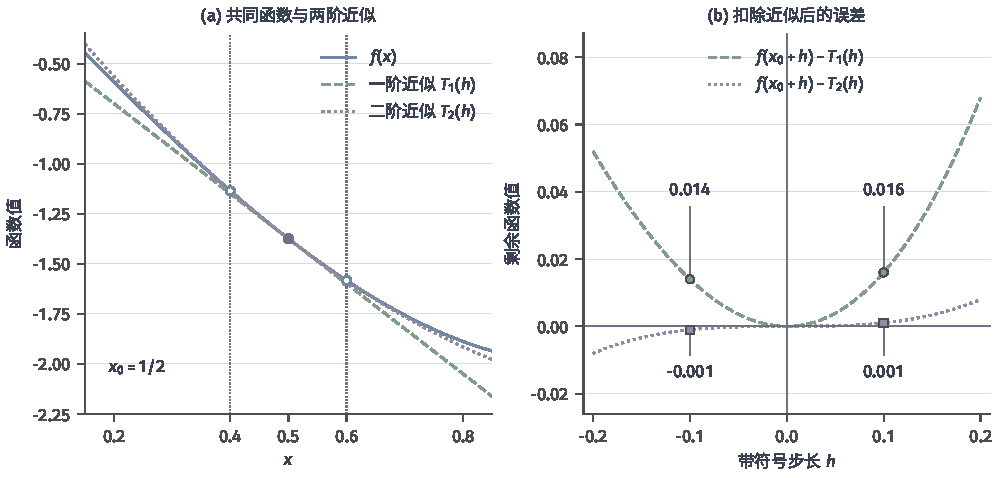
\includegraphics[width=169.0mm]{figures/01-mathematical-preliminaries-upper/01-mathematical-language-combinatorics-analysis-optimization/matplotlib/analysis-derivative-orders/figure.pdf}
  \caption{统一函数 $f(x)=x^3-3x$ 在 $x_0=1/2$ 处的两阶近似，记 $h=x-x_0$。（a）蓝线为真函数，绿虚线为切线近似 $T_1=f(x_0)+f'(x_0)h$，紫点线加入二次项 $f''(x_0)h^2/2$，得到 $T_2$。（b）扣除各近似后的带符号余项分别为 $3h^2/2+h^3$ 与 $h^3$，标出 $h=\pm0.1$ 的精确结果。一阶导数确定切线，二阶导数补充局部曲率；余项的正负表示真值位于近似值的哪一侧。图为解析教学示例。}
  \label{fig:analysis-derivative-orders}
\end{figure*}

\paragraph{多元展开与方向误差}

设连接$\bm{x}$与$\bm{x}+\bm{h}$的线段包含在一个开集内，并且$f$在该开集上二阶连续可微。对一元函数$\phi(t)=f(\bm{x}+t\bm{h})$使用Taylor定理，存在 $\theta\in(0,1)$使
\begin{equation}
  f(\bm{x}+\bm{h})
  =
  f(\bm{x})
  +\nabla f(\bm{x})^{\top}\bm{h}
  +\frac12
  \bm{h}^{\top}
  \nabla^2f(\bm{x}+\theta\bm{h})
  \bm{h}.
\label{eq:analysis-second-order-taylor}
\end{equation}
由Hessian矩阵的连续性，当$\bm{h}\to\bm{0}$时，中间点处的二阶项可以换成基点处的
二阶项，并把差异写成相对于$\lVert\bm h\rVert_2^2$趋零的余项：
\begin{equation}
  f(\bm{x}+\bm{h})
  =
  f(\bm{x})
  +\nabla f(\bm{x})^{\top}\bm{h}
  +\frac12\bm{h}^{\top}\nabla^2f(\bm{x})\bm{h}
  +o(\lVert\bm{h}\rVert_2^2).
\label{eq:analysis-second-order-local-model}
\end{equation}
式~\eqref{eq:analysis-second-order-local-model}是局部结论。若要在一个区域内给出统一余项界，还需控制该区域上的Hessian矩阵连续性或Lipschitz常数，不能仅凭一点处的二阶导数。

前面的Hessian判别需要的正是这种余项控制。下面把已陈述的正定与不定情形补成严格的函数值判断。

正定Hessian矩阵给出更强的充分条件：它要求每个方向都有正曲率，而不只是没有负曲率。
设$f$在$\bm{x}^{\star}$的某个邻域内二阶连续可微，
$\nabla f(\bm{x}^{\star})=\bm{0}$且
$\bm H_\star=\nabla^2f(\bm{x}^{\star})$正定。要把各方向的正曲率变成同一个正下界，
可以在单位球面上考察连续函数$\bm v\mapsto\bm v^\top\bm H_\star\bm v$。
单位球面紧致，故它取到最小值
\[
 \lambda=\min_{\lVert\bm v\rVert_2=1}\bm v^\top\bm H_\star\bm v>0.
\]
正定性保证取到的值仍为正。把任意非零$\bm h$除以其长度，就得到
$\bm h^\top\bm H_\star\bm h\geq\lambda\lVert\bm h\rVert_2^2$。
由Hessian矩阵的连续性，在足够小的球内有
$\lVert\nabla^2f(\bm x)-\bm H_\star\rVert_{\mathrm{op}}\leq\lambda/2$；
算子范数因而把二次型的变化量控制在$(\lambda/2)\lVert\bm h\rVert_2^2$以内，
邻近位置的曲率下界仍至少为$(\lambda/2)\lVert\bm h\rVert_2^2$。
用式~\eqref{eq:analysis-second-order-taylor}
的中间点表达式，即可把这个曲率下界变成函数值下界；具体地，充分靠近时有
\[   f(\bm{x}^{\star}+\bm{h})-f(\bm{x}^{\star})   \geq   \frac{\lambda}{4}\lVert\bm{h}\rVert_2^2>0 \]
对充分小的非零$\bm{h}$成立，故$\bm{x}^{\star}$是严格局部极小点。负定情形给出严格局部极大点。

若驻点处Hessian矩阵不定，分别选取二次型为正和为负的方向。
沿每个固定方向把扰动写成$t\bm v$时，余项为$o(t^2)$，因此充分小的非零$t$不会改变
非零二次项的符号，函数值因而分别增加和减小，该点称为\term{鞍点}（saddle point）。
例如$f(x,y)=x^2-y^2$的原点就是鞍点。
若Hessian矩阵仅半正定或半负定，且在某些非零方向上二次型为零，二阶判据可能没有结论，
必须查看更高阶项或函数的其他结构。上述必要条件还假定点位于无约束开集内部；
边界极小点的梯度可以不为零，受约束问题需要后续章节的可行方向与乘子条件。

\section{函数的积分与整体累计}
\label{sec:analysis-classical-integration}

微分描述一点附近怎样变化，积分研究一个范围内的数值怎样累计。困难是有限分割得到的和依赖分割与取样位置，必须证明细分后这些差别消失。下面先建立积分及其存在范围，再研究原函数、分步计算和坐标变换，最后沿路径和区域累计导数，说明端点与边界项来自哪里。这里采用有界区间与规则区域上的经典版本。

\subsection{积分的存在与累计范围}

从连续函数的面积累计开始，有限分割给出一组可核对的近似。上下和将所有取样选择夹在共同范围内，可积性要求这个范围能缩到任意小。建立有界区间上的积分后，再把无界函数和无穷区间作为截断极限处理。

\subsubsection{有界函数的分割累计}
\label{sec:analysis-riemann-integral}

\paragraph{黎曼和、上下和与分割细化}

要累计$f:[a,b]\to\mathbb R$在区间上的贡献，先选分割$P:a=x_0<x_1<\cdots<x_n=b$。在第$i$个小区间选取$\xi_i\in[x_{i-1},x_i]$，用矩形贡献$f(\xi_i)(x_i-x_{i-1})$代替这一段累计，得到\term{黎曼和}（Riemann sum）
\[
 S(f,P,\bm\xi)=\sum_{i=1}^n f(\xi_i)(x_i-x_{i-1}).
\]
暂时假定$f$有界，令$m_i=\inf_{[x_{i-1},x_i]}f$、$M_i=\sup_{[x_{i-1},x_i]}f$，便得到所有取样都满足的共同下界和上界：
\begin{equation}
 L(f,P)=\sum_i m_i(x_i-x_{i-1})
 \ \leq\ S(f,P,\bm\xi)\ \leq\
 U(f,P)=\sum_i M_i(x_i-x_{i-1}).
\label{eq:analysis-riemann-upper-lower-sums}
\end{equation}
增加分割点会提高下和或使它不变，降低上和或使它不变。不同分割可以取共同细化，因此任一下和不超过任一上和。若下和所能达到的上确界与上和所能达到的下确界相等，所有分割累计就确定同一个值。
\begin{definition}[黎曼可积与黎曼积分]
\label{def:analysis-riemann-integral}
设$a<b$且$f:[a,b]\to\mathbb R$有界。若
\[
 \sup_P L(f,P)=\inf_P U(f,P),
\]
则称$f$在$[a,b]$上\term{黎曼可积}（Riemann integrable），共同值称为\term{黎曼积分}（Riemann integral），记为$\int_a^b f(x)\,\mathrm dx$。
\end{definition}
等价的误差判据是：对每个$\varepsilon>0$都存在分割$P$使$U(f,P)-L(f,P)<\varepsilon$。共同值存在时，分别选出距它小于$\varepsilon/2$的下和与上和，再取共同细化即可证明这一方向；反过来，任一分割上的上下和差都控制两确界之差，所以任意小的差迫使它们相等。这也等价于分割的最大小区间长度趋零时，所有取样黎曼和趋向同一值；下面的存在性证明直接使用上下和判据。

若$f,g$均可积，细分同时控制两者在每个小区间的振荡，便可控制$f+g$的振荡。由有限和的线性并取极限，得到积分的线性。若$f\leq g$，每个黎曼和都保持次序，积分也保持次序。因此$|f-g|\leq M$时有$|\int_a^b f-\int_a^b g|\leq M(b-a)$。绝对值运算不扩大每段振荡，因此可积的$f$也有可积的$|f|$，且$|\int f|\leq\int|f|$。把一个区间分成相邻两段时，分割和相加，取极限也得到积分的区间可加性。这些性质把函数误差转成累计误差，后面会反复使用。

\paragraph{连续、有限跳变与不可积的对照}

若$f$在$[a,b]$上连续，紧致性先保证它有界且一致连续。给定$\varepsilon>0$，选$\delta>0$使两点相距小于$\delta$时函数值相差小于$\varepsilon/(b-a)$。当分割各段长度都小于$\delta$，每段的$M_i-m_i$不超过这一阈值，故
\[
 U(f,P)-L(f,P)=\sum_i(M_i-m_i)(x_i-x_{i-1})\leq\varepsilon.
\]
所以紧区间上的连续函数黎曼可积。这里一致连续负责同时控制全部小区间，只有逐点连续的定义尚不能直接选出共同分割尺度。

连续性是充分条件，不是必要条件。若有界函数只有有限个跳变，可以先用总长度任意小的短区间包住这些位置；它们对上下和差的贡献不超过函数振幅乘总长度。其余有限个闭区间上连续，再用一致连续控制。于是有限跳变仍可积，在有限个位置改值也不改变积分。

相反，令$d(x)=\mathbb I\{x\in\mathbb Q\}$，定义在$[0,1]$。每个非退化小区间都有有理数和无理数，因此每段$m_i=0$、$M_i=1$，任意分割都给出$L(d,P)=0$、$U(d,P)=1$。这个函数有界，却无法使上下累计接近，所以不黎曼可积。问题在于每一小段都保留最大振荡，而不是函数值很大。

\subsubsection{无界函数与无穷范围的累计}
\label{sec:analysis-improper-integrals}

\paragraph{反常积分的截断极限}

黎曼积分要求函数在有限闭区间上有界。若奇异性只发生在端点，可以先避开它再取极限。例如$f$在每个$[c,b]$（$a<c<b$）上黎曼可积，定义
\[
 \int_a^b f(x)\,\mathrm dx:=\lim_{c\downarrow a}\int_c^b f(x)\,\mathrm dx,
\]
前提是右侧存在有限极限。无穷区间则令$\int_a^\infty f=\lim_{R\to\infty}\int_a^R f$。这些通过截断建立的积分称为\term{反常积分}（improper integral）。有多个奇异端点或两端无穷时，应分别检查每一端，不能只用相互抵消的对称截断代替。

以正函数$x^{-p}$说明位置的重要性。对$p>0$，在$[2^k,2^{k+1}]$上的累计满足
\[
 2^{-p}2^{k(1-p)}\leq\int_{2^k}^{2^{k+1}}x^{-p}\,\mathrm dx\leq2^{k(1-p)}.
\]
这是把函数在该段的最小值和最大值分别乘区间长度。$p>1$时上界随$k$几何衰减，有限几何和有共同上界，所以尾部积分收敛；$0<p\leq1$时各段至少贡献一个不趋零的正量，累计发散。$p\leq0$时$x^{-p}\geq1$于$x\geq1$，也发散。

同样比较靠近$0$的各段$[2^{-(k+1)},2^{-k}]$，在$p>0$时累计介于$2^{k(p-1)}/2$与$2^{p-1}2^{k(p-1)}$之间，故局部累计恰在$p<1$时有限；$p\leq0$时函数还能连续延拓到$0$，本来就可积。于是$\int_0^1x^{-p}\,\mathrm dx$恰在$p<1$时有限，$\int_1^\infty x^{-p}\,\mathrm dx$恰在$p>1$时有限。这里仅用分段常数比较与有限几何和，不提前使用下一小节的原函数计算。

\paragraph{收敛、绝对收敛与尾部误差}

若$\int |f|$对应的反常积分有限，有限区间上的$|\int f|\leq\int|f|$就能统一控制任意两次截断的差。实数完备性保证$\int f$收敛，这称为绝对收敛。对非负函数，比较$f\leq g$且$\int g<\infty$即可得到收敛与尾部界。例如$p>1$时，按$[2^jR,2^{j+1}R]$分段比较得到
\[
 \int_R^{2^{K+1}R} x^{-p}\,\mathrm dx
 \leq R^{1-p}\sum_{j=0}^K 2^{j(1-p)}
 \leq\frac{R^{1-p}}{1-2^{1-p}},
\]
右侧与$K$无关，也就控制了整个无穷尾部；它随$R$增大而趋零，给出截断到$R$之后的误差。

正负抵消也可能产生有限极限。令$f(x)=(-1)^{k+1}/k$于$k\leq x<k+1$，其中$k=1,2,\ldots$。每个有限截断只含有限个跳变，整数端点的积分为$s_N=1-1/2+\cdots+(-1)^{N+1}/N$。偶数项$s_{2N}$递增且不超过$1$，所以有有限极限；相邻奇数项与其差为$1/(2N+1)\to0$，二者趋于同一值。非整数截断与相邻整数截断的积分差不超过$1/N$，因此$\int_1^\infty f$收敛。

但$\int_1^{N+1}|f|=\sum_{k=1}^N1/k$无界：从$k=2^j$到$2^{j+1}-1$的一组至少贡献$1/2$。所以这一反常积分收敛却不绝对收敛，正负贡献的抵消不可省略。后章的勒贝格可积要求绝对值累计有限，不能把这类条件收敛直接沿用为同一个可积判断。

\subsection{积分的计算与坐标变换}

积分定义解决了累计是否存在，但直接计算分割极限通常繁琐。先用原函数把区间累计变成端点差，再把多变量累计拆成分步计算，最后在更合适的坐标中改写函数与体积。每次变化都必须同时保留累计范围、方向和权重。

\subsubsection{区间积分的原函数计算}
\label{sec:analysis-integration-remainders}

\paragraph{累计函数与微积分基本定理}

先回顾微积分基本定理的连续版本。若$g$在$[a,b]$上连续，
$H(x)=\int_a^xg(t)\,\mathrm dt$在内点处满足$H'(x)=g(x)$；
若$H\in C^1([a,b])$，则$\int_a^bH'(x)\,\mathrm dx=H(b)-H(a)$。
这里$C^1$表示一阶连续可微，在闭区间端点采用单侧导数的连续延拓。
第一条可由
$[H(x+h)-H(x)]/h-g(x)=h^{-1}\int_x^{x+h}(g(t)-g(x))\,\mathrm dt$
和连续性得到；第二条再对$H(x)-H(a)-\int_a^xH'(t)\,\mathrm dt$
使用零导数蕴含常值的中值定理。这说明所用的是连续导数的积分，更一般的导数恢复条件将在第~\ref{chap:measurable-functions}章研究。

\paragraph{分部积分与积分余项}

有些乘积的积分难算，但把导数转移到另一个因子后会简化。分部积分就是这种转移规则，代价是增加边界贡献。若$u,v\in C^1([a,b])$，由乘积求导$(uv)'=u'v+uv'$并在$[a,b]$上积分，可得
\begin{equation}
  \int_a^b u(x)v'(x)\,\mathrm{d}x
  =
  [u(x)v(x)]_a^b
  -
  \int_a^b u'(x)v(x)\,\mathrm{d}x.
\label{eq:analysis-integration-by-parts}
\end{equation}
例如，取$u(x)=x$、$v'(x)=e^x$，得到 $\int_0^1xe^x\,\mathrm{d}x=[xe^x]_0^1-\int_0^1e^x\,\mathrm{d}x=1$。边界项不能无故删除；只有在函数于边界消失、区域无边界，或衰减速度足以使无穷远边界项趋零时才能省略。

分部积分还能把第~\ref{sec:analysis-taylor-approximation}节的局部二阶变化累计成有限位移的
余项。设连接$\bm{x}$与$\bm{x}+\bm{h}$的线段包含在一个开集内，且$f$在该开集上二阶
连续可微。令$\phi(t)=f(\bm{x}+t\bm{h})$，对$(1-t)\phi''(t)$在$[0,1]$上分部积分，得到
\[
  \int_0^1(1-t)\phi''(t)\,\mathrm{d}t
  =-\phi'(0)+\phi(1)-\phi(0).
\]
用链式法则代回，便得到不挑选中间点的Taylor积分余项：
\[   f(\bm{x}+\bm{h})   =   f(\bm{x})   +\nabla f(\bm{x})^{\top}\bm{h}   +   \int_0^1(1-t)   \bm{h}^{\top}\nabla^2f(\bm{x}+t\bm{h})\bm{h}\,\mathrm{d}t. \]
权重$1-t$说明越靠近位移起点的曲率贡献被累计得越多；该表达式与前面的中间点余项
描述同一有限变化，但保留了整条线段上的曲率信息。

一般阶数也由同一操作得到。设$f$在连接$x_0$和$x_0+h$的线段邻域内
$r+1$阶连续可微，$r\geq0$，令$\phi(t)=f(x_0+th)$。
记
\[
 I_r=\frac1{r!}\int_0^1(1-t)^r\phi^{(r+1)}(t)\,\mathrm dt.
\]
基本定理给出$I_0=\phi(1)-\phi(0)$；对$r\geq1$分部积分，
\[
 I_r=-\frac{\phi^{(r)}(0)}{r!}
       +\frac1{(r-1)!}\int_0^1(1-t)^{r-1}\phi^{(r)}(t)\,\mathrm dt
     =-\frac{\phi^{(r)}(0)}{r!}+I_{r-1}.
\]
逐次代入并用$\phi^{(k)}(0)=h^k f^{(k)}(x_0)$，便得
\begin{equation}
 f(x_0+h)=\sum_{k=0}^r\frac{f^{(k)}(x_0)}{k!}h^k
 +\frac{h^{r+1}}{r!}
   \int_0^1(1-t)^r f^{(r+1)}(x_0+th)\,\mathrm dt.
\label{eq:analysis-taylor-integral-remainder}
\end{equation}
参数化$x_0+th$同时处理正、负$h$。若$|f^{(r+1)}|\leq M$，积分权重的总量为
$1/(r+1)$，故余项不超过$M|h|^{r+1}/(r+1)!$，与前面的中间点余项界一致。
例如立方函数在$r=2$时有$f'''=6$，余项就是
$(h^3/2)\int_0^1 6(1-t)^2\,\mathrm dt=h^3$。
多元函数沿$\phi(t)=f(\bm x+t\bm h)$使用同一公式；$r=1$便还原前述Hessian积分余项。

\subsubsection{多变量积分的分步计算}

\paragraph{区域分割与体积累计}

在矩形$R=[a,b]\times[c,d]$上，分别划分两个坐标，把每个小矩形的面积乘以其中一个函数值后求和。若$f$在$R$上连续，紧致性给出统一振荡控制，所以分割细化时得到与取样无关的二重积分。更高维用小长方体体积作同样构造。

非矩形的有界区域$D$可以放入一个大矩形，把区域外的贡献设为零。这里采用规则区域：边界能用有限个光滑片段或曲面片描述，边界附近能够被总面积或总体积任意小的小块覆盖。这一条件保证边界小块对有界函数的上下和差贡献趋零。它是经典区域积分的条件，不要求事先建立一般集合的测度。

\paragraph{积分次序与区域描述}

矩形上的连续函数可以先按一个坐标累计，再按另一个坐标累计：
\[
 \int_R f(x,y)\,\mathrm d(x,y)
 =\int_a^b\left(\int_c^d f(x,y)\,\mathrm dy\right)\mathrm dx
 =\int_c^d\left(\int_a^b f(x,y)\,\mathrm dx\right)\mathrm dy.
\]
有限双重和本来就能交换相加次序；连续性提供共同的分割误差界，允许把这一关系传到积分极限。若区域写为$a\leq x\leq b$、$\alpha(x)\leq y\leq\beta(x)$，其中上下边界连续，内积分上下限就应使用$\alpha(x),\beta(x)$。改变积分次序时应重新描述同一个区域。

例如$D=\{(x,y):0\leq y\leq x\leq1\}$上累计$1$，先对$y$积分得到$\int_0^1\int_0^x1\,\mathrm dy\,\mathrm dx=1/2$；反过来，同一区域为$0\leq y\leq1$、$y\leq x\leq1$，故$\int_0^1\int_y^11\,\mathrm dx\,\mathrm dy=1/2$。若只交换微分符号而保留原来的限，就已经改变区域。一般可测函数或存在奇异抵消的情形，需要下一章的分步积分定理单独核验。

\subsubsection{坐标变化后的积分计算}
\label{sec:analysis-coordinate-change-integral-applications}

\paragraph{一元换元与链式法则}

设$g$在包含$T([a,b])$的区间上连续，$T\in C^1([a,b])$。取$g$的原函数$G$，链式法则给出$(G\circ T)'(x)=g(T(x))T'(x)$。再用基本定理得到
\[
 \int_a^b g(T(x))T'(x)\,\mathrm dx
 =G(T(b))-G(T(a))=\int_{T(a)}^{T(b)}g(u)\,\mathrm du.
\]
这里$\int_v^u=-\int_u^v$保留有向端点。若把换元理解为一一对应地累计普通长度，则还需在当前区间保证$T$单调，并用$|T'|$补偿方向翻转。

\paragraph{Jacobian与体积权重}

多元换元同时改变函数表达和小区域体积。设$D$是有界规则区域，$\overline D$包含在开集$U\subseteq\mathbb R^d$内；$T:U\to V$为一一对应的连续可微映射，其逆也连续可微，且$\det\bm J_T\neq0$。若$g$在$T(\overline D)$上连续，则经典换元公式为
\begin{equation}
 \int_{T(D)}g(\bm y)\,\mathrm d\bm y
 =\int_D g(T(\bm x))\left|\det\bm J_T(\bm x)\right|\,\mathrm d\bm x.
\label{eq:analysis-multivariate-change-variables}
\end{equation}
Jacobian描述局部线性变化，行列式的绝对值是普通体积的缩放比例。绝对值使坐标方向翻转后体积仍为正。公式可以从小块上的线性近似及统一误差控制证明；逐点线性化只说明局部缩放，严格的整体公式还要控制分割后的误差与像集重叠。这里陈述这一经典版本，后章再扩大到非负可测或绝对可积函数。

\begin{example}[极坐标中的面积权重]
\label{ex:analysis-polar-coordinate-jacobian}
令$D=\{\bm{x}\in\mathbb{R}^2:\lVert\bm{x}\rVert_2\leq1\}$，并令
$T(r,\theta)=(r\cos\theta,r\sin\theta)$。在开集
$(0,1)\times(0,2\pi)$上，$T$是到开圆盘内部去掉原点和正$x$轴径向接缝后的区域的
连续可微双射，逆映射也连续可微。其Jacobian矩阵的行列式为
\[   \det
\begin{bmatrix}     \cos\theta & -r\sin\theta\\     \sin\theta & r\cos\theta
\end{bmatrix}   =r. \]
为了避开原点和接缝，可先限制$\varepsilon\leq r\leq1-\varepsilon$、$\varepsilon\leq\theta\leq2\pi-\varepsilon$，在每个这样的闭矩形上使用经典换元。遗漏的中心小圆盘、外侧窄环与接缝窄扇形面积随$\varepsilon\downarrow0$趋零；对有界被积函数，它们的累计贡献也趋零。因此取极限得到
\[   \int_D1\,\mathrm{d}\bm{x}   =   \int_0^{2\pi}\int_0^1r\,\mathrm{d}r\,\mathrm{d}\theta   =\pi. \]
这里积分上下限包含端点不改变积分值。若参数化在一片有正面积或体积的区域上重复覆盖，则不能直接使用
上述双射版本，否则同一点会被重复计数。
\end{example}

图~\ref{fig:vol1-add-polar-area-weight}说明半径因子来自哪里。同样的角度变化在较大半径处扫过更长的弧，故同样大小的参数块对应更大的面积，积分权重必须随半径变化。
\begin{figure}[!htb]
  \centering
  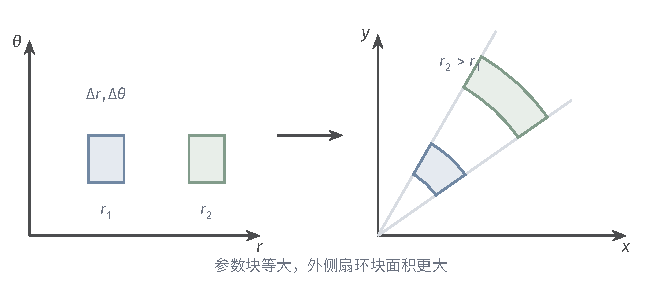
\includegraphics[width=112mm]{figures/01-mathematical-preliminaries-upper/01-mathematical-language-combinatorics-analysis-optimization/tikz/comprehension-additions/polar-area-weight.pdf}
  \caption{极坐标映射中的两个等大参数块，具有相同的$\Delta r,\Delta\theta$，但外侧半径$r_2$较大。对应扇环块的精确面积为$(r\Delta r+(\Delta r)^2/2)\Delta\theta$，一阶项为$r\Delta r\Delta\theta$，因此面积元为$r\,\mathrm dr\,\mathrm d\theta$。图只比较局部块，坐标原点与接缝的处理见正文。}
  \label{fig:vol1-add-polar-area-weight}
\end{figure}

\subsection{路径与区域中的边界关系}

前面在区域中累计函数值，现在改为累计导数。沿路径累计梯度留下端点差，在区域内累计散度留下边界净通量。两者都能由小段或小区域内部贡献相消理解，但方向、权重和光滑性条件不同，下面分别建立。

\subsubsection{路径累计与端点变化}

\paragraph{弧长累计与有向线积分}

换元仍是在同维区域内计算体积积分；如果贡献只沿一条路径累积，就应改用弧长或带方向的路径增量，不能继续套用全空间体积权重。设分段连续可微路径$\gamma:[a,b]\to\mathbb{R}^d$。对沿路径连续的标量函数
$h:\mathbb{R}^d\to\mathbb{R}$，标量线积分定义为
\[
  \int_\gamma h\,\mathrm{d}s
  =
  \int_a^b h(\gamma(t))\lVert\gamma'(t)\rVert_2\,\mathrm{d}t.
\]
速度的范数把参数增量换成弧长，因此反转路径方向不改变该积分。对沿路径连续的向量场
$\bm{F}:\mathbb{R}^d\to\mathbb{R}^d$，向量场线积分则定义为
\[   \int_{\gamma}\bm{F}\mathbin{\cdot}\mathrm{d}\bm{r}   =   \int_a^b   \bm{F}(\gamma(t))^{\top}\gamma'(t)\,\mathrm{d}t. \]

速度范数换算普通弧长，带方向的速度向量则保留行进方向。路径反向时，前者不变，后者变号；因此二者累计的是不同对象。

\paragraph{梯度场的端点差}

若$\bm{F}=\nabla\phi$且$\phi$连续可微，链式法则给出
\begin{equation}
  \int_{\gamma}\nabla\phi\mathbin{\cdot}\mathrm{d}\bm{r}
  =
  \phi(\gamma(b))-\phi(\gamma(a)).
\label{eq:analysis-line-integral-gradient}
\end{equation}
因此梯度场的路径积分只依赖端点。向量场线积分在路径方向反转时变号；若漏掉参数化导数
$\gamma'(t)$，就会丢失方向和行进速度的信息。

\begin{example}[同一路径上的长度、端点差与环流]
\label{ex:analysis-path-integral-comparison}
取单位圆的上半圆路径$\gamma(t)=(\cos t,\sin t)$，$0\leq t\leq\pi$。
它的速度范数恒为$1$，所以$\int_\gamma1\,\mathrm ds=\pi$。
取$\phi(x,y)=x$，则$\nabla\phi=(1,0)^\top$，
\[
 \int_\gamma\nabla\phi\mathbin{\cdot}\mathrm d\bm r
 =\int_0^\pi-\sin t\,\mathrm dt=-2
 =\phi(-1,0)-\phi(1,0).
\]
换成旋转场$\bm F(x,y)=(-y,x)^\top$时，
$\bm F(\gamma(t))^\top\gamma'(t)=1$，沿上半圆的积分为$\pi$。
但沿同样端点的直径路径$\eta(t)=(1-2t,0)$，$0\leq t\leq1$，
内积恒为零，积分为$0$。向量场连续甚至光滑，也不能单独保证路径无关。
沿完整单位圆逆时针一周，这个旋转场的积分为$2\pi$；梯度场沿闭合路径的端点差
必须为零，所以它不可能在整个平面上写成一个连续可微势函数的梯度。
\end{example}

\subsubsection{区域累计与边界通量}

\paragraph{散度与内部贡献相消}

路径积分沿行进方向累计，通量则计算穿过边界的贡献。在向量场
$\bm F=(F_1,\ldots,F_d)^\top$中，散度定义为
$\nabla\mathbin{\cdot}\bm F=\sum_{i=1}^d\partial F_i/\partial x_i$；
它把各坐标方向的局部流出率相加。相邻小区域的公共边界法向相反，
内部交换在总和中相消，剩下的应是外边界的净流出。


对一个小长方体，每个坐标方向上两面的净流出约等于该方向的偏导数乘体积。把小块相加，内部公共面的法向相反，所以贡献抵消；只有外边界保留下来。

\paragraph{散度定理与多元分部积分}

以下采用经典的规则区域版本：$\Omega$是有界开区域，其边界由有限个$C^1$
曲面片组成，每个光滑片附近区域位于边界的一侧，片间接缝可以被总边界面积任意小的细片覆盖。
光滑区域、多边形和通常的多面体均符合这一条件。若向量场$\bm{F}$
在$\overline{\Omega}$的一个开邻域内连续可微，
\term{散度定理}（divergence theorem）写成
\begin{equation}
  \int_{\Omega}\nabla\mathbin{\cdot}\bm{F}\,\mathrm{d}\bm{x}
  =
  \int_{\partial\Omega}\bm{F}^{\top}\bm{n}\,\mathrm{d}S,
\label{eq:analysis-divergence-theorem}
\end{equation}
其中$\bm{n}$是外单位法向量，$\mathrm dS$表示边界上的面积元素。这个公式把区域内部与区域边界两种积分联系起来；左边汇总区域内部的局部流出率，右边计算穿过边界的净通量。普通多边形角点和多面体接缝已包含在上述分片条件内。对于不满足上述分片及局部单侧条件的边界，或涉及无界区域、弱导数的情形，需要另用相应版本并重新核对边界项。分部积分、路径积分与散度定理共同说明，局部导数进入整体积分时， 通常会留下不可忽略的边界信息。

例如单位开圆盘$\Omega$上的$\bm F(x,y)=(x,y)^\top$有散度$2$，
故左边为$2\pi$。边界参数化$\gamma(t)=(\cos t,\sin t)$，$0\leq t\leq2\pi$，
外单位法向就是$\bm n=\gamma(t)$，弧长元素为$\mathrm dS=\mathrm dt$；
因此$\bm F^\top\bm n=1$，右边也为$2\pi$。
改用内法向会得到$-2\pi$，这不是同一定理中的方向约定。
前例的旋转场散度为零，且在圆周上始终与法向垂直，所以通量为零，
尽管沿切向的环流为$2\pi$。这一区别说明线积分和通量计算的不是同一种贡献。

取连续可微标量函数$u,v$，令$\bm F=u\nabla v$，并假定$v$二阶连续可微。乘积法则给出$\nabla\mathbin\cdot(u\nabla v)=\nabla u^\top\nabla v+u\Delta v$，其中$\Delta v=\sum_i\partial^2v/\partial x_i^2$称为Laplace算子。代入散度定理得
\[
 \int_\Omega u\Delta v\,\mathrm d\bm x
 =\int_{\partial\Omega}u\nabla v^\top\bm n\,\mathrm dS
  -\int_\Omega\nabla u^\top\nabla v\,\mathrm d\bm x.
\]
这个多元分部积分公式将二阶导数转给另一个因子，同时保留法向边界项；边界条件是否使该项为零，需要在具体问题中判断。

\section{函数逼近与运算的极限}
\label{sec:analysis-function-convergence-essential-bounds}

现在让被研究的函数本身随索引变化。固定一个输入后仍是一列数，但各位置的趋近速度可以不同，积分还会累计误差发生的范围。下面先规定函数列的共同误差尺度，再分别检查连续性、积分和求导是否保留，最后研究部分和与更新规则生成的特殊逼近。经典方法失效的反例将明确引出下一章的任务。

\subsection{函数列的误差尺度与极限存在}

逐点误差只检查一个位置，一致误差要求同一轮近似控制全部位置。先用幂函数列分清这两个量词次序，再用一致柯西条件判断未知函数极限的存在。这里不要求输入已经有距离，也不要求各函数连续或可积。

\subsubsection{逐点误差与统一误差}

\paragraph{各位置分别趋近}

固定一个输入以后，比较的只是一列实数。这里不需要函数可微或可积，甚至不需要
在输入集合上指定距离；函数值仍按实数绝对值比较。
\begin{definition}[逐点收敛]
\label{def:analysis-pointwise-almost-everywhere-convergence}
设$f_n,f:X\to\mathbb{R}$。若
\[
 \begin{gathered}
  \forall x\in X,\quad
  \forall\varepsilon>0,\quad
  \exists N=N(x,\varepsilon)\in\mathbb N,\\
  \forall n\geq N,\quad
  |f_n(x)-f(x)|<\varepsilon,
 \end{gathered}
\]
即对每个$x$都有$\lim_n f_n(x)=f(x)$，称$f_n$逐点收敛到$f$。
\end{definition}


例如$f_n(x)=x^n$在$[0,1]$上，对每个$x<1$趋于$0$，在$x=1$却始终等于$1$。所以逐点极限为$f(x)=0$（$x<1$）、$f(1)=1$；这一写法先固定位置，再让$n$增加。

\paragraph{整个范围的共同控制}

即使每个输入处的误差最终都很小，开始稳定的时刻仍可能依赖输入。
若希望一次选定迭代次数后就控制全部输入，需要更强的一致条件。

这个区别不是纯粹的技术细节。实际使用近似函数时，通常要先决定计算到第几轮，
再把这个近似函数交给下一步使用；而逐点收敛只保证每个位置最终会变准，不保证在
固定的轮数上处处都准。一致收敛正是允许“先定轮数、再要求处处达标”的条件。
\begin{definition}[函数列的一致收敛]
\label{def:analysis-uniform-convergence}
设$X$为非空集合，$f_n,f:X\to\mathbb R$。若
\[
  \forall\varepsilon>0,\quad
  \exists N=N(\varepsilon)\in\mathbb N,\quad
  \forall x\in X,\quad
  \forall n\geq N,\quad
  |f_n(x)-f(x)|<\varepsilon,
\]
就称$f_n$在$X$上一致收敛到$f$。等价地，
\begin{equation}
  \lVert f_n-f\rVert_{\infty}
  :=
  \sup_{x\in X}|f_n(x)-f(x)|
  \longrightarrow0.
\label{eq:analysis-uniform-convergence}
\end{equation}
这里的上确界检查全部输入，不排除任何位置。
\end{definition}


两条定义的区别落在量词次序。逐点收敛允许$N$依赖$x$；一致收敛把$\exists N$
移到$\forall x$之前，同一个$N$必须同时控制全部输入。区别不在“趋近”这个词，
而在误差阈值之后允许谁依赖谁。下面用同一列函数比较这两种控制。

在$[0,1]$上取$f_n(x)=x^n$。它逐点收敛到
\[
 f(x)=
 \begin{cases}
  0,&0\leq x<1,\\
  1,&x=1.
 \end{cases}
\]
每个固定的$0<x<1$都有$x^n\to0$，端点$1$处的函数值与极限值则始终都为$1$，误差为零。
但对每个$n$，$\sup_{x\in[0,1]}|f_n(x)-f(x)|=\sup_{0\leq x<1}x^n=1$，所以收敛不一致。
从量词看，固定$\varepsilon=1/2$后，无论选多大的$N$，在$n=N$时
总能选$x_N=(3/4)^{1/N}<1$，使误差$x_N^N=3/4>\varepsilon$。
失败的位置可以随$n$移动；不能把“每个位置最终变小”改写成“某一轮以后所有位置都小”。
若把范围缩为$[0,a]$，其中$0\leq a<1$，则上确界误差为$a^n\to0$，同一公式又变成一致收敛。

\subsubsection{未知极限函数时的收敛判断}

\paragraph{一致柯西条件}

前面都先给出候选极限，再判断误差；实际构造时可能只知道后面的函数彼此很近。
令$S$为任意非空集合，$\mathcal F_{\mathrm b}(S)$为所有有界实函数$S\to\mathbb{R}$的集合，配备普通上确界范数
\[   \lVert f\rVert_{\infty}   =   \sup_{x\in S}|f(x)|. \]
这里的元素是整个函数，距离比较它们在全部输入上的最大误差。
所比较的是两个函数之间的距离$\lVert f-g\rVert_\infty$，它检查每个输入而不排除例外位置。
一致柯西条件就是
\[
 \forall\varepsilon>0,\quad\exists N,\quad
 \forall m,n\geq N,\quad\forall x\in S,\quad
 |f_m(x)-f_n(x)|<\varepsilon.
\]

\paragraph{一致极限的存在与归属}

这个空间完备。事实上，若$(f_n)$满足上述条件，对每个固定$x$，
$(f_n(x))$是实柯西列，故存在$f(x)=\lim_n f_n(x)$。
取一个$n_0$使$\lVert f_n-f_{n_0}\rVert_\infty\leq1$对所有充分大的$n$成立，
再令$n\to\infty$，得到$|f(x)|\leq|f_{n_0}(x)|+1$，所以$f$有界。
对任意$\varepsilon>0$，选$N$使$m,n\geq N$时
$\lVert f_m-f_n\rVert_\infty<\varepsilon/2$。固定$n\geq N$并令$m\to\infty$，
对所有$x$都有$|f(x)-f_n(x)|\leq\varepsilon/2$，于是
$\lVert f-f_n\rVert_\infty\leq\varepsilon/2<\varepsilon$。
这证明$f_n$在该空间中收敛到$f$，而不只是分别得到了各个点的极限。

\subsection{极限下的性质与运算保持}

误差尺度确定后，还需分别检查希望保留的对象。连续性只用函数值的三角误差分解，积分会累计整个范围，求导还会把相邻位置的差除以很小的位移。因此三个保持问题需要各自证明，不能由其中一个自动推出另两个。

\subsubsection{连续性是否保留}

\paragraph{一致极限的连续性}

前面的完备性说明一致柯西列有函数极限，还可以追问原函数的性质是否保留。
若度量空间$X$上的实函数$f_n$连续，且$f_n$一致收敛到$f$，则$f$连续。
固定$x\in X$与$\varepsilon>0$，先选$n$使$\lVert f-f_n\rVert_\infty<\varepsilon/3$，
再由这个$f_n$在$x$处连续，选$\delta>0$控制
$|f_n(x')-f_n(x)|<\varepsilon/3$。于是$d(x,x')<\delta$时，
\[
 |f(x')-f(x)|
 \leq |f(x')-f_n(x')|+|f_n(x')-f_n(x)|+|f_n(x)-f(x)|
 <\varepsilon.
\]
一致误差同时控制两端，连续性才被保留。仅逐点收敛没有这个共同控制；上面的$x^n$
例子中，各项连续，极限在$x=1$处却不连续。这里回用的是第~\ref{sec:analysis-continuous-limits}节的连续性，并未使用积分。

\paragraph{逐点极限中的跳变}

一致收敛是这个结论的充分条件，不是极限连续的必要条件。
例如$x^n$在$[0,1)$上的逐点极限恒为零，仍然连续，但其上确界误差始终为$1$。
这不反驳上面的定理，只说明有些不满足统一误差条件的函数列也恰好保留了连续性。

同一幂函数列在闭区间上的极限于$1$处不连续。每个固定位置最终准确仍然不够，因为靠近$1$的困难位置随$n$不断移动，找不到共同轮数来完成连续性证明中的两端误差控制。

\subsubsection{积分是否可以交换极限}
\label{sec:analysis-classical-limit-integral}

\paragraph{有限区间上的一致误差界}

设$f_n$在固定区间$[a,b]$上黎曼可积，并一致收敛到$f$。先说明极限仍可积：固定一个使$\lVert f-f_n\rVert_\infty<\eta$的$n$，则任意分割$P$满足
\[
 U(f,P)-L(f,P)
 \leq U(f_n,P)-L(f_n,P)+2\eta(b-a).
\]
先选$\eta$控制第二项，再利用$f_n$可积选分割控制第一项，即可把差压到任意小。由积分的大小关系，进一步有
\begin{equation}
 \left|\int_a^bf_n(x)\,\mathrm dx-\int_a^bf(x)\,\mathrm dx\right|
 \leq(b-a)\lVert f_n-f\rVert_\infty\longrightarrow0.
\label{eq:analysis-uniform-riemann-limit}
\end{equation}
固定有限区间把统一点值误差转成累计误差。若只知逐点收敛，就没有右侧可用的共同上界；若区间无穷长，也不能直接乘一个有限长度来完成估计。

\paragraph{连续尖峰中的贡献集中}

用同一形状比较两列连续函数。对$n\geq2$，在$[0,1]$上定义三角尖峰
\[
 \psi_n(x)=\max\{1-|2nx-1|,0\}.
\]
它在$[0,1/n]$外为零，顶点位于$1/(2n)$，高度为$1$。对每个固定$x>0$，充分大的$n$使$x>1/n$，而$x=0$处始终为零，所以$\psi_n\to0$处处成立。其面积为底宽乘高度再除以二，即$\int_0^1\psi_n=1/(2n)\to0$，但$\lVert\psi_n\rVert_\infty=1$，并不一致收敛。

只把高度改为$2n$，令$h_n=2n\psi_n$。每个固定位置仍然最终为零，可是
\begin{equation}
 \int_0^1 h_n(x)\,\mathrm dx=1,
 \qquad \int_0^1\lim_{n\to\infty}h_n(x)\,\mathrm dx=0.
\label{eq:analysis-continuous-spike-integral-failure}
\end{equation}
两列都由连续函数组成并处处趋零，差别只在收窄范围的同时是否提高了高度。逐点极限看不到随$n$移动的峰顶，积分却累计其整个面积。第一列说明一致收敛不是积分交换的必要条件，第二列说明逐点收敛不足以保证交换。下一章将用共同可积控制解释两者差别。

\subsubsection{求导是否可以交换极限}

\paragraph{函数值接近而导数不接近}

连续性保留不意味着变化率也保留。原因在于导数由差商定义，而差商用到同一个函数在两个
不同位置的值：一致收敛控制的是每个位置上的误差，差商相减时两处的误差却可能以相反方向
放大。下面的两个反例分别从尖点和振荡说明差别。
用平滑函数
\[   f_{\varepsilon}(x)=\sqrt{x^2+\varepsilon^2},   \qquad \varepsilon>0 \]
在$\varepsilon\downarrow0$时逼近$|x|$。由
\[   0\leq f_{\varepsilon}(x)-|x|   =   \frac{\varepsilon^2}   {\sqrt{x^2+\varepsilon^2}+|x|}   \leq\varepsilon, \]
可知$f_{\varepsilon}$在整个$\mathbb{R}$上一致收敛到$|x|$。其导数为
\[   f_{\varepsilon}'(x)   =   \frac{x}{\sqrt{x^2+\varepsilon^2}}. \]
对每个$x\neq0$，导数收敛到$\operatorname{sign}(x)$；在$x=0$处始终为$0$，而$|x|$
在那里没有导数。即使人为规定$\operatorname{sign}(0)=0$，导数收敛也不一致。例如取
$x_\varepsilon=\varepsilon^2>0$，则
\[
  f_\varepsilon'(x_\varepsilon)
  =
  \frac{\varepsilon}{\sqrt{1+\varepsilon^2}}
  \longrightarrow0,
  \qquad
  \operatorname{sign}(x_\varepsilon)=1.
\]
因此两者之差的绝对值趋于$1$，不可能一致收敛。所以函数值的一致逼近不能推出导数的一致逼近。
讨论光滑近似时，必须明确控制的是函数值、导数还是积分误差。
振荡还给出另一个不依赖不可微点的障碍。令
$f_n(x)=\sin(nx)/n$，$x\in[0,2\pi]$，则
$\lVert f_n\rVert_\infty\leq1/n\to0$，但$f_n'(x)=\cos(nx)$不一致趋于零，
甚至在$x=0$始终为$1$。高频振荡使函数幅度趋零，斜率幅度却保持不变。
若目标是近似导数，必须直接控制导数误差或补充保证导数收敛的条件；只增加函数值的精度
并不能消除高频振荡。

\paragraph{导数误差与单点锚定}

若直接控制导数，则可以反过来保证函数与导数一起收敛；还需在一个位置固定函数值，
以免遗漏任意的竖直平移。下面给出闭区间上的一个便于核对的版本。
\begin{theorem}[一致导数逼近与求导保持]
\label{thm:analysis-uniform-derivative-limit}
设$a<b$，$f_n\in C^1([a,b])$。若存在$x_0\in[a,b]$使$f_n(x_0)\to c$，
且$f_n'$在$[a,b]$上一致收敛到$g$，则$f_n$在$[a,b]$上一致收敛到
\[
 f(x)=c+\int_{x_0}^xg(t)\,\mathrm dt.
\]
函数$f$连续，并在$(a,b)$内可微，满足$f'=g$。
\end{theorem}
\begin{proof}
各$f_n'$连续，前面的连续性保持结论说明其一致极限$g$连续。
微积分基本定理给出$f_n(x)=f_n(x_0)+\int_{x_0}^xf_n'(t)\,\mathrm dt$，因此
\[
 \sup_{x\in[a,b]}|f_n(x)-f(x)|
 \leq |f_n(x_0)-c|+(b-a)\lVert f_n'-g\rVert_\infty
 \longrightarrow0.
\]
连续的$g$可积，微积分基本定理又给出内点处$f'(x)=g(x)$。
\end{proof}
定理回用微分与闭区间积分，不需要支配收敛。若不控制$f_n(x_0)$，
$f_n(x)=n$的导数虽恒为零，函数值却没有有限极限；若不控制导数的统一误差，
前面的振荡例子则会阻断求导保持。

\subsection{累计与迭代生成的逼近}

前面的函数列没有规定生成方式。部分和把每项规定为已有累计加上新增项，迭代则把下一项规定为当前状态经过更新映射。加入这些结构后，可以由尾和或压缩因子直接计算误差；带扰动更新还需把每一步新增偏差按传播权重累计。

\subsubsection{部分和的极限与截断误差}

\paragraph{级数收敛与绝对收敛}

数列$(a_n)$记录一组按索引排列的数；级数研究的是把这些数依次相加后的累计结果：单步误差是否变小，与这些误差累计起来是否有限，是两个不同的问题。第~\ref{chap:sets-functions-and-proofs}章的有限和只加到指定的$N$，得到
\[
  s_N=\sum_{n=1}^{N}a_n=a_1+a_2+\cdots+a_N.
\]
$s_N$称为\term{部分和}（partial sum）。让$N$不断增加，又得到一个新的数列
$(s_N)$：原数列的每一项是$a_n$，新数列的每一项是前$N$项的总和。符号
\term{无穷级数}（infinite series）$\sum_{n=1}^{\infty}a_n$描述的正是这一求和过程；
只有当部分和数列有有限极限$s$时，才称级数收敛，并把这个极限记作
$\sum_{n=1}^{\infty}a_n=s$。

例如，$a_n=2^{-n}$作为数列趋于$0$，对应的部分和却是
$s_N=1-2^{-N}$，趋于$1$。这两个极限回答不同的问题：单个新增项是否变小，以及全部
新增项的累计量是否稳定。把两者联系起来的是$s_N-s_{N-1}=a_N$：新增项正是部分和的
一步增量，所以部分和稳定必然要求新增项趋零。取$s_0=0$，级数收敛因此推出
$a_n=s_n-s_{n-1}\to0$，但单项趋零并不足够。例如调和级数$\sum_{n=1}^{\infty}1/n$发散。把从$2^k$到$2^{k+1}-1$的项分成一组，该组有$2^k$项，每项至少为$1/2^{k+1}$，所以每组之和至少为$1/2$；部分和因而可以超过任意给定常数。

当$|r|<1$时，有限几何和
\[   \sum_{n=0}^{N}r^n=\frac{1-r^{N+1}}{1-r} \]
在$N\to\infty$时给出
\begin{equation}
  \sum_{n=0}^{\infty}r^n=\frac{1}{1-r}.
\label{eq:analysis-geometric-series}
\end{equation}
$|r|<1$不可删去：$r=1$时部分和不断增长，$r=-1$时部分和振荡，$|r|>1$时单项甚至不趋于零。折扣回报和几何误差界都依赖这一条件。

计算只能取有限项，因此还要知道遗漏的尾部有多大。若级数收敛到$s$，记
$R_N=s-s_N$；能用非负尾和控制$|R_N|$时，截断误差就有统一估计，不必依赖正负误差的偶然相消。
若$\sum_n|a_n|<\infty$，就称级数\term{绝对收敛}（absolutely converge）。由式~\eqref{eq:analysis-cauchy-tail-bound}对应的尾和估计，绝对收敛蕴含收敛。回到柯西条件，若$\sum_k|a_{k+1}-a_k|$收敛，其尾和就能统一控制任意$m>n$的差，从而保证$(a_n)$是柯西数列。绝对收敛还允许重新排列求和次序而保持级数的和；只有条件收敛时，重排可能改变和甚至使其发散。第~\ref{chap:measurable-functions}章的分步积分结论将给出这一原则在积分中的对应形式。

\paragraph{尾和控制与求和安排}

具体地，$|R_N|\leq\sum_{n>N}|a_n|\to0$。任意重排只要已经包含原来前$N$项，
其尚未计算的贡献就都来自这个绝对尾和，故不会改变最终的和。
收敛但不绝对收敛称为条件收敛，例如$\sum_{n\geq1}(-1)^{n+1}/n$；
正项总和与负项绝对值总和都发散，改动二者进入部分和的次序便可能改变相消结果。
这个例子也说明，有限和的交换律不能不加条件地搬到无穷和。

下面的步长例子用到$p$级数$\sum_{n\geq1}n^{-p}$：它恰在$p>1$时收敛。
不借助积分也能核对这一条件。对$p>0$，第$k$组$n=2^k,\ldots,2^{k+1}-1$的和
介于$2^{-p}2^{k(1-p)}$与$2^{k(1-p)}$之间；$p>1$时可用几何级数控制，
$0<p\leq1$时各组之和不趋于零。$p\leq0$时原级数的单项已不趋于零。

设第$t$步计算产生非负误差$\delta_t$。“单步误差趋零”只表示$\delta_t\to0$； “前$T$步累计误差”是$\sum_{t=0}^{T-1}\delta_t$；“误差可求和”则要求 $\sum_{t=0}^{\infty}\delta_t<\infty$。三者不能混用。例如 $\delta_t=1/(t+1)$逐步趋零，但累计误差无界；$\delta_t=1/(t+1)^2$才可求和。若误差进入第~\ref{chap:sets-functions-and-proofs}章式
\eqref{eq:prelim-perturbed-recurrence}那样的稳定递推，较早误差还会被几何权重衰减， 此时应分析加权累计量，而不是只看$\delta_t$本身。

在迭代更新$x^{(t+1)}=x^{(t)}+\alpha_t v_t$中，$v_t$给出本轮更新方向，$\alpha_t$决定走多远，称为步长。若步长过快缩小，总行进尺度可能有限；若噪声影响随步长平方累计，又希望平方和有限。这就使同一个步长序列承担“持续前进”和“抑制平方误差”两项职责。典型条件
\[   \sum_{t=1}^{\infty}\alpha_t=\infty,   \qquad   \sum_{t=1}^{\infty}\alpha_t^2<\infty \]
可由$\alpha_t=1/t$满足：第一项是调和级数，第二项是收敛的$p$级数。这里尚不能据此推出随机算法收敛，因为还缺少噪声和目标函数的条件；这个例子只说明两个累计对象可以有不同结论。后续分析折扣、步长和扰动时，都应先问清趋零的是哪一项、累计采用什么权重， 以及所需级数是否真的收敛。


第~\ref{sec:comb-growth-scales}节用大$O$和小$o$比较规模；这里的收敛使小$o$中的比值趋零
有了明确含义。若$b_n>0$最终成立，$a_n=o(b_n)$要求$a_n/b_n\to0$，不仅要求
比值有界。例如$1/n=O(1/n)$，却不是$o(1/n)$；$1/n^2=o(1/n)$。
比较误差时必须固定趋向和分母尺度，不能由单项趋零推出累计可求和。

以上的数项也可以依赖输入。若$|a_n(x)|\leq M_n$对所有$x$成立，且$\sum_nM_n<\infty$，则任意尾部都满足
\[
 \sup_x\left|\sum_{n=N+1}^{K}a_n(x)\right|\leq\sum_{n>N}M_n\longrightarrow0.
\]
部分和因此一致柯西，得到一致极限。连续项的和连续；在有限区间上，可积项的和还可交换求和与积分。这里保证这些结论的是统一的可求和上界，并不是仅有每个位置上的级数收敛。

\subsubsection{压缩更新的收敛与停止判断}
\label{sec:analysis-complete-contraction}

\paragraph{不动点、压缩条件与唯一极限}

更新规则$x^{(t+1)}=T(x^{(t)})$可以算出每个有限步状态，但算出很多项并没有证明它们趋于一个解。
数值计算中反复做同一件事（如牛顿法、迭代求平方根）时，自然会问：迭代会不会停在某个点、
那个点是不是想要的解、离它还有多远？与任意点列或部分和不同，这里的极限不再是一个给定的数，而要由一个方程间接刻画：若迭代确实收敛到$x^\star$，对上式的两端取极限就会得到$x^\star=T(x^\star)$。因此收敛性证明必须同时完成两件事：说明序列有极限，说明这个极限满足方程。若更新把任意两点的距离统一缩小，就能把相邻状态的距离累积成有限几何尾和，从而证明序列是柯西序列。还需要空间完备，才能让所得极限留在允许范围内；更新的连续性再保证极限满足$x=T(x)$。这里回用两项工具：前面的级数给出几何尾和的界，开篇的完备性给出极限的归属。


寻找更新方程的解，就是寻找更新前后不再变化的点：把当前估计再代入一次$T$，估计不再改变，
算法自然应当停止，这样的点称为不动点。
\begin{definition}[不动点]
\label{def:analysis-fixed-point}
设$T:X\to X$为映射。点$x^\star\in X$若满足$T(x^\star)=x^\star$，就称为$T$的不动点（fixed point）。
\end{definition}

仅有不动点方程尚不能判断迭代是否接近它。下面要求同一次更新把任意两点之间的距离按共同因子缩小，由此统一控制相邻迭代的差。
\begin{definition}[压缩映射]
\label{def:analysis-contraction}
设$(X,d)$为度量空间。映射$T:X\to X$若存在$q\in[0,1)$使
\begin{equation}
  d(Tx,Ty)\leq qd(x,y)
  \quad\text{对所有 }x,y\in X,
\label{eq:analysis-contraction-definition}
\end{equation}
就称为\term{压缩映射}（contraction mapping）。
\end{definition}
关键是同一个$q<1$在整个所考察空间上成立，并且$T$确实把$X$映回自身
\scite{math-conway1990functional}
\begin{theorem}[Banach压缩映射定理]
\label{thm:analysis-banach-fixed-point}
设$(X,d)$是非空完备度量空间，$T:X\to X$为压缩映射，压缩因子为$q<1$。则$T$有
唯一不动点$x^\star\in X$。从任意$x^{(0)}\in X$出发定义
$x^{(n+1)}=T(x^{(n)})$，都有$x^{(n)}\to x^\star$，并且
\begin{align}
  d(x^{(n)},x^\star)
  &\leq
  \frac{q^n}{1-q}d(x^{(1)},x^{(0)}),
\label{eq:analysis-banach-apriori-error}\\
  d(x^{(n)},x^\star)
  &\leq
  \frac{q}{1-q}d(x^{(n)},x^{(n-1)})
  \quad(n\geq1).
\label{eq:analysis-banach-aposteriori-error}
\end{align}
\end{theorem}
\begin{proof}
反复使用压缩条件可得
\[   d(x^{(n+1)},x^{(n)})   \leq   q^n d(x^{(1)},x^{(0)}). \]
对$m>n$，三角不等式和几何级数给出
\begin{align*}
  d(x^{(m)},x^{(n)})
  &\leq
  \sum_{k=n}^{m-1}d(x^{(k+1)},x^{(k)})\\
  &\leq
  d(x^{(1)},x^{(0)})\sum_{k=n}^{m-1}q^k\\
  &\leq
  \frac{q^n}{1-q}d(x^{(1)},x^{(0)}).
\end{align*}
右边随$n\to\infty$趋于零，所以$(x^{(n)})$是柯西数列。完备性保证存在
$x^\star\in X$使$x^{(n)}\to x^\star$。由压缩条件与三角不等式，
\begin{align*}
 d(Tx^\star,x^\star)
 &\leq d(Tx^\star,Tx^{(n)})+d(x^{(n+1)},x^\star)\\
 &\leq qd(x^\star,x^{(n)})+d(x^{(n+1)},x^\star)
 \longrightarrow0.
\end{align*}
左侧不依赖$n$，故$T(x^\star)=x^\star$。

若$y^\star$也是不动点，则
\[   d(x^\star,y^\star)   =   d(Tx^\star,Ty^\star)   \leq qd(x^\star,y^\star). \]
因为$q<1$，只能有$d(x^\star,y^\star)=0$，故不动点唯一。

在上面的柯西界中令$m\to\infty$，便得式~\eqref{eq:analysis-banach-apriori-error}。若从第$n-1$步重新计算同一界，
\[   d(x^{(n)},x^\star)   \leq   \sum_{k=n}^{\infty}d(x^{(k+1)},x^{(k)})   \leq   d(x^{(n)},x^{(n-1)})\sum_{j=1}^{\infty}q^j, \]
便得到式~\eqref{eq:analysis-banach-aposteriori-error}。
\end{proof}

这个证明同时说明存在、唯一和可计算的误差界各来自哪里：几何尾和使迭代为柯西列， 完备性把极限留在空间中，压缩距离估计使极限成为不动点，严格的$q<1$保证唯一性。若只允许$q=1$，结论都可能丢失。恒等映射$T(x)=x$有无穷多个不动点； $T(x)=x+1$在$\mathbb{R}$上没有不动点，且相应迭代发散。非扩张并不等于压缩。
完备性也不能省略。在非完备空间$X=(0,1)$上，映射$T(x)=x/2$是压缩因子为
$1/2$的自映射，但它唯一可能的不动点是被排除的$0$。从任意$x^{(0)}\in X$出发，
迭代$x^{(n)}=x^{(0)}/2^n$在$\mathbb{R}$中趋于$0$，却不在$X$中收敛。

\paragraph{先验误差与后验误差}

先验界在计算前给出所需步数，后验界则使用已经算出的相邻两步距离。
例如在$\mathbb R$上取$T(x)=x/2+1$、$x^{(0)}=0$，则$q=1/2$，
$x^{(1)}=1$，唯一不动点为$2$。先验界给出
$|x^{(n)}-2|\leq2^{1-n}$；要求误差不超过$10^{-3}$时，$n=11$已足够。
后验界在这里化为
$|x^{(n)}-2|\leq|x^{(n)}-x^{(n-1)}|$，无需事先知道答案$2$就能停止。
一般$q$接近$1$时，因子$q/(1-q)$可能很大，“相邻两步已经很近”不能独自作为
到解误差很小的证据。$q=0$时映射为常值，一步即到不动点。


图~\ref{fig:vol1-add-contraction-cobweb}把同一压缩例子的计算步骤画成折线。竖段完成求值$T(x)$，横段把所得数值复制为下一轮的自变量；折线逐步接近两条曲线相交的不动点。
\begin{figure}[!htb]
  \centering
  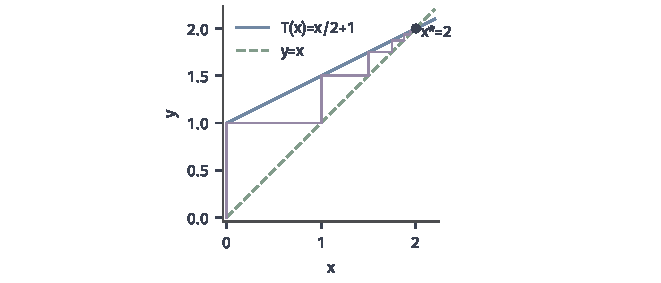
\includegraphics[width=112mm]{figures/01-mathematical-preliminaries-upper/01-mathematical-language-combinatorics-analysis-optimization/matplotlib/comprehension-additions/contraction-cobweb.pdf}
  \caption{$T(x)=x/2+1$在$[0,2]$上的七步迭代，初值$x^{(0)}=0$。蓝线是$T$，绿虚线是恒等函数，紫折线交替完成求值与复制；交点为$x^\star=2$。精确迭代为$x^{(n)}=2-2^{1-n}$，图中几何收缩对应压缩因子$1/2$。}
  \label{fig:vol1-add-contraction-cobweb}
\end{figure}

\paragraph{隐式方程的局部不动点构造}

现在可以补全定理~\ref{thm:analysis-implicit-function}的构造证明。把方程的线性化逆作为校正，使待解变量上的更新在基点处导数为零；再缩小邻域，同时核对统一压缩与自映射。这个顺序同时保证解存在、局部唯一和可微，形式求导只能给出最后的候选公式。

\begin{proof}
为证明定理~\ref{thm:analysis-implicit-function}的存在性，先把方程改写为局部压缩迭代。记
\[   \bm{A}   =   \bm{D}_{\bm{y}}F(\bm{a},\bm{b}),   \qquad   T_{\bm{x}}(\bm{y})   =   \bm{y}-\bm{A}^{-1}F(\bm{x},\bm{y}). \]
$F(\bm{x},\bm{y})=\bm{0}$当且仅当$\bm{y}$是$T_{\bm{x}}$的不动点。并且
\[   \bm{D}_{\bm{y}}T_{\bm{x}}(\bm{y})   =   \bm{I}   -   \bm{A}^{-1}\bm{D}_{\bm{y}}F(\bm{x},\bm{y}), \]
它在$(\bm{a},\bm{b})$处为零。由导数连续性，可以选择闭球 $B=\{\bm{y}:\lVert\bm{y}-\bm{b}\rVert_2\leq r\}$和$\bm{a}$的邻域$U$，使
\begin{equation}
  \sup_{\bm{x}\in U,\,\bm{y}\in B}
  \left\lVert
    \bm{D}_{\bm{y}}T_{\bm{x}}(\bm{y})
  \right\rVert_{\mathrm{op}}
  \leq q<1.
\label{eq:analysis-ift-uniform-contraction}
\end{equation}
沿$\bm{y}$方向使用式~\eqref{eq:analysis-operator-mean-value-bound}可知，每个
$T_{\bm{x}}$在$B$上都是同一因子$q$的压缩映射。

还必须核对自映射。因为$T_{\bm{a}}(\bm{b})=\bm{b}$且$T_{\bm{x}}(\bm{b})$关于 $\bm{x}$连续，可进一步缩小$U$，使
\[   \lVert T_{\bm{x}}(\bm{b})-\bm{b}\rVert_2   \leq\frac{1-q}{2}r. \]
于是对$\bm{y}\in B$，
\[
  \lVert T_{\bm{x}}(\bm{y})-\bm{b}\rVert_2
  \leq
  q\lVert\bm{y}-\bm{b}\rVert_2+\frac{1-q}{2}r
  \leq
  \frac{1+q}{2}r
  <r.
\]
所以$T_{\bm{x}}(B)$包含在$B$的内部$V$中。闭球$B$在有限维欧氏空间中完备，Banach
定理便对每个$\bm{x}\in U$给出唯一不动点$\varphi(\bm{x})\in V$。若
$(\bm{x},\bm{y})\in U\times V$且$F(\bm{x},\bm{y})=\bm{0}$，则$\bm{y}\in B$也是
$T_{\bm{x}}$的不动点，唯一性迫使$\bm{y}=\varphi(\bm{x})$。这证明了定理所述的局部
存在与零点集合的逐点唯一性。

还需说明所得解随参数连续可微。把$U$进一步缩小为开球，并使
$\overline U\times B$包含在原定义域内；这个集合紧致，关于$\bm x$的导数连续，
故有统一范数上界$L$。对$\bm x,\bm x'\in U$，
两点间的线段仍在$U$内，式~\eqref{eq:analysis-operator-mean-value-bound}
可用于$T_{\bm x}(\bm y)$的参数变化。利用两个不动点关系，
\[   \lVert\varphi(\bm{x})-\varphi(\bm{x}')\rVert_2   \leq   q\lVert\varphi(\bm{x})-\varphi(\bm{x}')\rVert_2   +L\lVert\bm{x}-\bm{x}'\rVert_2, \]
移项得到$\lVert\varphi(\bm x)-\varphi(\bm x')\rVert_2
\leq L\lVert\bm x-\bm x'\rVert_2/(1-q)$，
故$\varphi$局部Lipschitz连续。令 $\bm{h}\to\bm{0}$并记 $\bm{k}=\varphi(\bm{x}+\bm{h})-\varphi(\bm{x})$，前述界给出 $\lVert\bm{k}\rVert_2=O(\lVert\bm{h}\rVert_2)$。对恒等式
\[   F(\bm{x}+\bm{h},\varphi(\bm{x})+\bm{k})   -   F(\bm{x},\varphi(\bm{x}))   =   \bm{0} \]
作一阶展开，得到
\[   \bm{D}_{\bm{x}}F\,\bm{h}   +   \bm{D}_{\bm{y}}F\,\bm{k}   +   o(\lVert\bm{h}\rVert_2)   =   \bm{0}. \]
展开中的Jacobian均在$(\bm x,\varphi(\bm x))$处取值，联合扰动的余项
$o(\lVert(\bm h,\bm k)\rVert_2)$因$\lVert\bm k\rVert_2=O(\lVert\bm h\rVert_2)$
成为$o(\lVert\bm h\rVert_2)$。
基点的$\det\bm A\neq0$，行列式又是矩阵元素的连续函数，
所以邻域足够小时$\bm D_{\bm y}F$仍可逆。于是
\[   \bm{k}   =   -   (\bm{D}_{\bm{y}}F)^{-1}   \bm{D}_{\bm{x}}F\,\bm{h}   +   o(\lVert\bm{h}\rVert_2). \]
这证明$\varphi$可微并给出式~\eqref{eq:analysis-implicit-derivative}；各Jacobian矩阵连续又保证$\bm{D}\varphi$连续。至此，隐函数定理中的存在、局部唯一与导数公式都已得到说明。证明中特别核对了自映射和统一压缩条件，只有形式上的固定点改写并不足够。
\end{proof}

\subsubsection{带扰动更新的误差累计}

\paragraph{单步误差的传播权重}

精确更新的压缩性不代表数值实现没有误差。实际迭代几乎总有偏差：用小批量样本估计的更新方向、
浮点舍入、提前停止都会让每一步没有恰好落在$T(x^{(t)})$上。需要回答的是，这些每轮新增的
偏差会被迭代逐步消化，还是累积成一个无法消除的误差底。设$T$满足压缩条件，精确轨迹为
$x^{(t+1)}=T(x^{(t)})$，计算轨迹为$z^{(t)}$，且每次更新满足
$d(z^{(t+1)},T(z^{(t)}))\leq\delta_t$，其中$\delta_t\geq0$。
令$e^{(t)}=d(z^{(t)},x^{(t)})$，三角不等式给出
\begin{equation}
 \begin{aligned}
 e^{(t+1)}
 &\leq d(z^{(t+1)},T(z^{(t)}))
       +d(T(z^{(t)}),T(x^{(t)}))\\
 &\leq\delta_t+\rho e^{(t)},\qquad 0\leq\rho<1.
 \end{aligned}
\label{eq:analysis-perturbed-distance-recursion}
\end{equation}
这里$\rho$就是所用压缩因子。对到不动点的误差$d(z^{(t)},x^\star)$也有同一递推。
把不等式逐次代入，或对$t$归纳，得到
\begin{equation}
 e^{(t)}
 \leq \rho^t e^{(0)}
       +\sum_{s=0}^{t-1}\rho^{t-1-s}\delta_s.
\label{eq:analysis-perturbed-distance-unrolling}
\end{equation}
这正是第~\ref{chap:sets-functions-and-proofs}章式~\eqref{eq:prelim-unrolled-recurrence}
的有限展开在距离误差中的应用；本章再判断它随$t$增加的行为。
若$\delta_s\leq\bar\delta$，则
$e^{(t)}\leq\rho^t e^{(0)}+\bar\delta(1-\rho^t)/(1-\rho)$，
所以$\limsup_t e^{(t)}\leq\bar\delta/(1-\rho)$。
这是最坏误差范围，不是断言每条计算轨迹都收敛到这个上界。

\paragraph{持续扰动与衰减扰动}

展开式中的旧误差会衰减，每轮新增误差则继续进入累计。固定初值与压缩系数，只改变新增误差是否趋零，就能看清两种误差来源。
\begin{example}[持续扰动与衰减扰动]
\label{ex:prelim-recurring-perturbations}
取$e^{(0)}=1$、$\rho=1/2$，并暂把递推中的不等号取为等号。若每步都加入
$\delta_t=0.1$，展开式给出
\[
 e^{(t)}=2^{-t}+0.1\sum_{s=0}^{t-1}2^{-s}
        =0.2+0.8\,2^{-t}.
\]
初始误差逐步消失，持续加入的误差却留下$0.2$的极限。若改为
$\delta_t=0.1/(t+1)$，扰动本身也衰减，稳定递推便使$e^{(t)}\to0$。
例如第$1$步两者都是$0.6$，第$2$步分别为$0.4$和$0.35$；差别来自第二步加入的
新误差，而不是初值不同。这里的$1/(t+1)$扰动并不可求和，几何权重仍能使其累计影响趋于零；可求和性是更强的条件。
\end{example}

\begin{figure}[htbp]
  \centering
  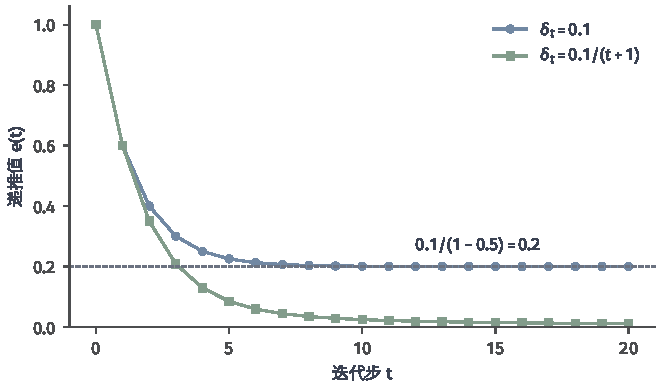
\includegraphics[width=112.0mm]{figures/01-mathematical-preliminaries-upper/01-mathematical-language-combinatorics-analysis-optimization/matplotlib/prelim-perturbed-recurrence/figure.pdf}
  \caption{相同初值与收缩系数下的两种递推。蓝线使用持续扰动，绿线使用衰减扰动；每个点都是整数步上的精确递推值，图中$e(t)$对应正文的$e^{(t)}$，灰虚线是持续扰动留下的极限$0.2$。图为教学构造。}
 \label{fig:prelim-perturbed-recurrence}
\end{figure}

衰减扰动的结论可以直接由有限展开式~\eqref{eq:analysis-perturbed-distance-unrolling}核对。
给定$\varepsilon>0$，先选$S$使$s\geq S$时$\delta_s\leq\varepsilon(1-\rho)/2$。
对$t>S$把累计和拆成两段：前$S$项是有限个旧扰动，其权重随$t$几何趋零；后面的项满足
\[
 \sum_{s=S}^{t-1}\rho^{t-1-s}\delta_s
 \leq\frac{\varepsilon(1-\rho)}2\sum_{j=0}^{t-1-S}\rho^j
 \leq\frac\varepsilon2.
\]
旧扰动项和初始误差在充分大的$t$后也不超过$\varepsilon/2$，因此总误差趋于零。
这里需要$0\leq\rho<1$、$\delta_s\to0$和有限的初始误差；只写“每步误差很小”仍不足够。

函数逼近还可能超出原积分范围。枚举$[0,1]$内的有理数为$q_1,q_2,\ldots$，令$E_n=\{q_1,\ldots,q_n\}$，$g_n=\mathbb I_{E_n}$。每个$g_n$仅在有限个位置不连续，黎曼积分为零；它逐点递增到$d=\mathbb I_{\mathbb Q\cap[0,1]}$，而第~\ref{sec:analysis-riemann-integral}节已证明$d$不黎曼可积。这次困难是极限对象失去原来的可积性；连续尖峰的极限仍然可积，却发生积分交换失败。下一章需要分别扩大积分范围，并建立对整个逼近过程的控制条件。

\section{本章小结}
\label{sec:analysis-summary}

距离说明何谓接近，完备性保证柯西逼近的终点仍在空间内，闭性则保留额外的范围约束。连续性把输入极限传到输出，紧致定义域进一步提供极值达到和统一变化控制。微分在此基础上描述局部变化，有限位移与高阶近似还需要导数界和余项条件。

积分从有限分割的共同累计建立。连续性保证紧区间上的黎曼可积，却不是可积性的必要条件；换元、分部积分及边界公式分别保留体积权重、端点项和法向方向。它们共同把局部变化联系到整体累计，所采用的经典版本均有明确的范围与光滑性条件。

函数列把这些条件重新放到极限中检验。一致误差能保留连续性及有限区间上的积分，却不能独自保证求导交换；导数一致误差还需一个位置的函数值作为锚点。部分和与压缩迭代利用各自生成结构提供误差界，扰动递推则区分单步误差与累计影响。有限点示性函数列和连续尖峰留下两项任务：为更多极限函数建立积分，并控制贡献随逼近移动、集中或消失的情形。这将成为可测函数章的起点。

\chapter{最优化}
\label{chap:optimization}

第~\ref{chap:mathematical-analysis}章给出了函数的局部变化和极限条件。若任务要求从所有允许参数中选出目标值最小的一个，局部变化能提供怎样的求解信息，计算出的候选又凭什么算作足够好？本章用带正则项的最小二乘与资源约束追踪这两个问题。设训练样本有$n\geq1$个，参数为$\bm w\in\mathbb R^d$，观测值组成$\bm y=(y_1,\ldots,y_n)^\top\in\mathbb R^n$，矩阵$\bm X$的第$i$行为预测输入$\bm x_i^\top$。拟合目标为
\begin{equation}
  F(\bm{w})
  =
  \frac{1}{2n}\lVert \bm{X}\bm{w}-\bm{y}\rVert_2^2
  +\frac{\lambda}{2}\lVert\bm{w}\rVert_2^2,
  \qquad
  \bm{X}\in\mathbb{R}^{n\times d},\quad \lambda\geq 0,
  \label{eq:opt-regularized-least-squares}
\end{equation}
以及线性资源约束
\begin{equation}
  \bm{A}\bm{w}=\bm{b},\qquad
  \bm{G}\bm{w}\leq\bm{h}.
  \label{eq:opt-linear-resource-constraints}
\end{equation}
式~\eqref{eq:opt-regularized-least-squares}与第~\ref{chap:sets-functions-and-proofs}章的
式~\eqref{eq:prelim-regularized-least-squares}是同一个目标的矩阵写法。正则项限制参数
规模，约束则直接排除超出预算的候选；两者看似都在“限制模型”，却改变了不同的数学对象。

同一个目标值误差可以由不同方法取得，但方法需要的信息与计算成本不同。光滑目标允许用梯度和曲率构造方向，非光滑项可能需要保留在可解子问题中，约束则要求同时核验候选的可行性。预算有限时，还可以改变每步读取的信息、变量范围或子问题精度；多个评价目标则需要另行规定怎样选择答案。这些条件可以同时出现，本章按“先确认问题有解，再选择利用什么信息”的顺序展开：第~\ref{sec:opt-objectives-solutions-curvature}节只回答最优解是什么、何时存在、局部信息能推出多少全局结论，不涉及具体算法；其后各节才按可用信息分类选择求解方法。为了固定比较口径，除拟合与资源两个例子之外，本章还使用以下二次目标
\begin{equation}
 f(\bm w)=\frac12(w_1^2+16w_2^2),\qquad
 \bm H=\operatorname{diag}(1,16),\qquad
 \bm w^{(0)}=(2,2)^\top.
 \label{eq:opt-common-quadratic}
\end{equation}
其最小点为零、初始目标值为$34$；两方向曲率的差异使方向、步长和每步成本都能直接核算。

\section{优化问题的定义与基本性质}
\label{sec:opt-objectives-solutions-curvature}

目标有下界并不保证最优值能够达到，梯度为零也不保证候选已经最优。求解之前，需要分别建立解的含义、最优值达到的条件，以及局部比较能够推出哪些全局结论。存在性使用极限与可行域性质，凸性和曲率条件则连接局部信息、解的唯一性与误差界。后面的算法将各自调用这些保证。

\subsection{优化问题与解}
\label{sec:opt-problem-and-solutions}
\label{sec:opt-error-objects}

把实际问题写成优化问题，要做的是四项约定：哪些量可以调整（变量），允许取值到什么范围（可行域），按什么准则比较两个候选（目标函数），以及是否要求达到最优还是只需足够好。
这一步看似只是套格式，实际上回答的是“机器到底被允许做什么、按什么打分”：训练模型时
变量是参数，可行域可能是预算或非负约束，打分是损失；同一个业务诉求若把其中任何一项
换一种写法，求出来的就可能是另一个决策。四项里任何一项写得不同，得到的答案就可能不同。例如同样想“让误差小”，若可行域写成整个空间，最优参数可能无界；若写成某个有界集合，答案就落在集合内；若比较准则改成绝对误差而不是平方误差，最优点也可能移动。因此优化问题的完整写法是

一个优化问题必须同时给出目标函数、变量和可行域。记
\[
  \min_{\bm{w}\in C}F(\bm{w}),\qquad
  C=\{\bm{w}\in\mathbb{R}^d:
  \bm{A}\bm{w}=\bm{b},\ \bm{G}\bm{w}\leq\bm{h}\}.
\]
变量$\bm w$是待选择的参数，目标$F$规定怎样比较候选，可行域$C$规定哪些候选允许采用。
若等式有$m$条、不等式有$p$条，则
$\bm A\in\mathbb R^{m\times d}$、$\bm b\in\mathbb R^m$、
$\bm G\in\mathbb R^{p\times d}$、$\bm h\in\mathbb R^p$，向量不等式逐坐标理解。
若$C=\varnothing$，问题\term{不可行}（infeasible）；若$C\neq\varnothing$但
$\inf_{\bm{w}\in C}F(\bm{w})=-\infty$，问题\term{无下界}（unbounded below）。
只有可行且有有限下界，才值得继续问下确界是否由某个点达到。
例如同时要求$x\leq0$和$x\geq1$就不可行；
在实线上最小化$x$无下界，$\inf_{x\in\mathbb R}e^x=0$有下界却没有最小点；
把$x$限制在$[0,1]$后，后一问题的最小值变为$1$且在$0$达到。
最优值是数$F^\star=\inf_C F$，最优解集合是$\argmin_C F$，后者可以为空或包含多个点。
写出问题$\min_C F$表示求最小值的任务，并不代替存在性证明；
声称某个数等于$\min_C F$时，才需要确认它确实被可行点取得。可行的判别方式是分开报告
两件事：最优值是多少，以及是否有可行点达到它。例如$\min_{w\in[0,1]}w$的最优值$0$
由$w=0$取得；$\min_{w>0}w$的最优值仍为$0$，却没有点取得，因为可行域不含$0$。
两种情形下最优值相同，可用的结论完全不同。

\begin{definition}[全局解、局部解与无约束驻点]
\label{def:opt-solutions-stationarity}
设$C\subseteq\mathbb R^d$非空，$F:C\to\mathbb R$。\term{全局最优解}（global minimizer）$\bm{w}^{\star}\in C$满足
$F(\bm{w}^{\star})\leq F(\bm{w})$对所有$\bm{w}\in C$成立。\term{局部最优解}
（local minimizer）要求存在$r>0$，使该不等式对所有
$\bm w\in C\cap B(\bm w^\star,r)$成立。
无约束可微问题的\term{驻点}（stationary point）满足
$\nabla F(\bm{w})=\bm{0}$。驻点只是局部一阶变化消失，可能是极小点、极大点或
第~\ref{sec:analysis-second-order-curvature}节所说的微分鞍点。
\end{definition}
给定$\varepsilon>0$和可行候选$\widehat{\bm w}\in C$，若
\[
  F(\widehat{\bm{w}})-\inf_{\bm{w}\in C}F(\bm{w})\leq\varepsilon,
\]
就称$\widehat{\bm{w}}$为目标值意义下的$\varepsilon$近似解。对无约束可微问题，
另一种常见标准是
$\lVert\nabla F(\widehat{\bm{w}})\rVert_2\leq\varepsilon$；在没有额外曲率条件时，
这两种近似不能互换。一般约束问题的精确最优点也可能有非零梯度；
后面的约束求解将建立同时反映允许移动方向与可行性的停止标准。

只报一个停止量而不说明它衡量什么，会掩盖实际精度。小梯度说明当前点附近已经没有
值得利用的一阶方向，却不说明离最优值还有多远；小目标差说明接近最优值，却不说明参数
是否唯一；参数距离小则依赖参照解的选择。三种量在不同的曲率条件下互相控制，下面先看
它们在一维的分化。取
$f(x)=\epsilon x^2/2$、$\epsilon=10^{-8}$；在$x=10^6$处，
梯度只有$0.01$，目标值却比最小值高$5000$，到最小点$0$的距离仍为$10^6$。
平坦方向把一阶变化压得很小，因此梯度停止标准首先回答的是局部变化是否足够小。
把小梯度换成小目标差，还需要梯度与目标差之间的定量条件；
把目标差换成参数距离，又需要相应的曲率下界。后文将分别建立这些界，
使用时必须同时带上它们的常数。

前面的目标值近似标准只比较目标与最优值之间的差距。评价同一个近似参数时，还可以关心它离某个参照参数多远，
或者它的预测发生了多大变化。这三个问题要分别选择误差对象。
下面暂取$C=\mathbb{R}^d$，不加资源约束，以式~\eqref{eq:opt-regularized-least-squares}为目标。
令$F^\star=\inf_{\bm{w}\in\mathbb{R}^d}F(\bm{w})$；若选定一个最小点
$\bm{w}^\star$，则
\[
  F(\widehat{\bm{w}})-F^\star,\qquad
  \lVert\widehat{\bm{w}}-\bm{w}^\star\rVert_2,\qquad
  \left(
    \frac{1}{n}\sum_{i=1}^{n}
    \bigl(
      \widehat{\bm{w}}^{\top}\bm{x}_i
      -(\bm{w}^\star)^{\top}\bm{x}_i
    \bigr)^2
  \right)^{1/2}
\]
分别是目标值误差、参数误差和在给定样本输入上的预测误差。最小点不唯一时，参数误差还
需要指定参照解，或改成到最小点集合的距离。三种误差衡量不同对象，彼此能否控制取决于
目标曲率、数据矩阵和参数化；一个误差较小不能无条件推出另两个也较小。

例如，在$n=1$、$\bm{x}_1=(1,0)^\top$、$y_1=0$、$\lambda=0$时，
目标函数为$F(w_1,w_2)=w_1^2/2$。参照解$(0,0)$与参数$(0,100)$的目标值都为$0$，
在这个样本输入上的预测也相同，参数距离却是$100$。差别来自目标和当前观测都没有约束
第二个坐标；并不是把目标误差算得更精确就能补回这项信息。

若希望在一个目标式中同时比较代价并排除不可行点，可以约定不可行点的代价为$+\infty$。
这种扩展实值表达把约束并入函数，后面的非光滑子问题就不必另写一套可行域符号。
\begin{definition}[适当函数、有效定义域与约束指标]
\label{def:opt-proper-domain-indicator}
函数$f:\mathbb R^d\to\mathbb R\cup\{+\infty\}$若不恒为$+\infty$，称为适当函数；
它从不取$-\infty$。其\term{有效定义域}（effective domain）为
$\operatorname{dom}f=\{\bm x:f(\bm x)<+\infty\}$。
集合$C$的扩展实值指标函数为$\iota_C(\bm x)=0$（$\bm x\in C$），在其余点取$+\infty$。
\end{definition}
它不同于前文计数与分析中使用的指示函数$\mathbb I\{\cdot\}$：后者在条件成立时取$1$、
否则取$0$，只给集合成员作标记；$\iota_C$在$C$外取$+\infty$，把不允许的点排除出最小化。
于是$\min_{\bm w\in C}F(\bm w)$可统一写成
$\min_{\bm w\in\mathbb R^d}\{F(\bm w)+\iota_C(\bm w)\}$。
有限惩罚只是不喜欢违规候选，$+\infty$才真正将它排除。有效定义域记录有有限代价的点，
适当性保证至少还有一个这样的点；它不保证有下界、更不保证最小值达到。

\subsection{最优解的存在}
\label{sec:opt-existence}

在讨论怎样求解之前，必须先确认所要找的对象存在。一个下确界可能由可行点达到，也可能只是逼近而达不到；若连最优点都不存在，任何算法返回的候选都不可能是它。判断存在性的通用做法甚至不需要算法：即使暂时不知道如何求解，也能选择一列目标值越来越接近下确界的候选，称为最小化序列。
有限下确界$m$时，可逐项选取$F(\bm w^{(k)})\leq m+1/k$；若下确界为$-\infty$，
则可逐项要求$F(\bm w^{(k)})\leq-k$。要从这些候选得到最优点，须回答三个问题：
序列能否取到收敛子列，极限是否仍可行，目标值比较能否传到极限。
若$C\subseteq\mathbb{R}^d$非空且紧，$F:C\to\mathbb{R}$连续，则
定理~\ref{thm:analysis-extreme-value}保证$F$在$C$上达到全局最小值。这里直接复用
第~\ref{chap:mathematical-analysis}章的极值存在结论。

可行域不紧时，目标本身也可能阻止最小化序列逃向无穷远。
\begin{definition}[强制性与下半连续性]
\label{def:opt-coercive-lower-semicontinuous}
设$C\subseteq\mathbb R^d$，$F:C\to(-\infty,+\infty]$。若沿$C$中的任意序列，
$\lVert\bm{w}\rVert_2\to\infty$时$F(\bm{w})\to\infty$，称$F$是
\term{强制的}（coercive）。$F$在$C$上\term{下半连续}
（lower semicontinuous）要求对每个收敛序列
$\bm{w}^{(k)}\to\bm{w}$都有
\[
  F(\bm{w})\leq\liminf_{k\to\infty}F(\bm{w}^{(k)}).
\]
其中序列与极限点均属于$C$。
\end{definition}
连续性并不是存在性证明所需的最弱条件。下半连续性允许函数值在极限点向下跳，
却不允许极限点的函数值突然高于邻近值。等价地，每个
下水平集$\{\bm{w}\in C:F(\bm{w})\leq a\}$在$C$的相对拓扑中都是闭集。

设$C$非空且闭，$F:C\to(-\infty,+\infty]$下半连续、强制，并且不恒为
$+\infty$且从不取$-\infty$。取$\bar{\bm{w}}\in C$使
$F(\bar{\bm{w}})<+\infty$，再把最小化序列限制到下水平集
\[
  K=\{\bm{w}\in C:F(\bm{w})\leq F(\bar{\bm{w}})\}.
\]
若$\inf_C F=F(\bar{\bm{w}})$，则$\bar{\bm{w}}$已经是最小点；否则
$\inf_C F<F(\bar{\bm{w}})$，任一最小化序列从某项起都落入$K$，可以只保留这段尾序列。
强制性使$K$有界，下半连续性与$C$的闭性使$K$闭，故$K$在有限维空间中紧。该尾序列
有子列收敛到$\bm{w}^{\star}\in K$，而下半连续性给出
$F(\bm{w}^{\star})\leq\liminf_kF(\bm{w}^{(k)})=\inf_C F$。因此下确界达到。
若原先假设下确界为$-\infty$，同一不等式会迫使$F(\bm w^\star)=-\infty$，
与适当性矛盾；所以这些条件也排除了无下界情形。
这个证明也指出各条件的职责：强制性阻止序列逃向无穷远，闭性保留可行极限，下半连续性
把目标值比较传到极限点。
当$\lambda>0$时，式~\eqref{eq:opt-regularized-least-squares}满足
$F(\bm{w})\geq\lambda\lVert\bm{w}\rVert_2^2/2$，所以即使可行域无界也不会沿参数
无穷大的方向降低目标。这里的推理顺序是：先用下界排除无下界情形，再用强制性得到有界的
下水平集，最后由闭性和下半连续性把极限留在可行域内。三项目标各自对应一个条件，
缺少任何一项都可能让最小化序列逃向无穷远或边界。

\subsection{凸性条件下的最优解性质}
\label{sec:opt-convexity}

\subsubsection{凸性与全局最优}

局部最优只比较附近候选；要把这项保证扩展到全部可行域，需要让远处更优的候选也能影响附近的比较。
为什么普通函数做不到这一点？设想目标里有两个互相隔开的山谷，站在其中一个谷底向四周看
都更高，局部上它已经最优，但另一处山谷可能更低；局部信息里完全没有远处山谷的线索。
若任意两个可行点之间的线段都可行，而且沿线段的目标值不超过两端值的加权平均，那么只要
远处有一个更低的点，连向它的整条线段都不能高于两端连线，当前点附近就一定存在更低的点，
从而排除“假谷底”。这两项条件分别是集合与函数的凸性。
\begin{definition}[凸集与凸函数]
\label{def:opt-convex-set-function}
集合$C\subseteq\mathbb R^d$为\term{凸集}（convex set），是指对任意
$\bm{u},\bm{v}\in C$和$\theta\in[0,1]$，
$\theta\bm{u}+(1-\theta)\bm{v}\in C$。线性等式、线性不等式和范数球的解集都是凸集，
它们的交集仍为凸集，所以式~\eqref{eq:opt-linear-resource-constraints}定义凸可行域。

定义在凸集$C$上的函数$f:C\to\mathbb R$若对任意$\bm u,\bm v\in C$和$\theta\in[0,1]$满足
\begin{equation}
  f(\theta\bm{u}+(1-\theta)\bm{v})
  \leq
  \theta f(\bm{u})+(1-\theta)f(\bm{v}),
  \label{eq:opt-convex-function}
\end{equation}
就称为\term{凸函数}（convex function）。若$-f$凸，则称$f$凹。
\end{definition}
凸函数的函数图像位于任意弦段下方。若远处存在更小的函数值，连向该点的线段就会在当前点附近给出更小的值\scite{math-boyd2004convex}

\begin{theorem}[凸函数的一阶与二阶判据]
\label{thm:opt-convexity-criteria}
设$C$为开凸集。可微函数$f:C\to\mathbb{R}$凸，当且仅当对任意
$\bm{u},\bm{v}\in C$，
\begin{equation}
  f(\bm{v})\geq f(\bm{u})
  +\langle\nabla f(\bm{u}),\bm{v}-\bm{u}\rangle.
  \label{eq:opt-first-order-convexity}
\end{equation}
若$f$二阶可微，则这又等价于
$\nabla^2f(\bm{w})\succeq\bm{0}$对所有$\bm{w}\in C$成立。
\end{theorem}

\begin{proof}
若$f$凸，令$\phi(t)=f(\bm{u}+t(\bm{v}-\bm{u}))$。由凸性，
$[\phi(t)-\phi(0)]/t\leq\phi(1)-\phi(0)$。令$t\downarrow0$便得
式~\eqref{eq:opt-first-order-convexity}。反过来，令
$\bm{z}=\theta\bm{u}+(1-\theta)\bm{v}$，分别把一阶不等式用于
$(\bm{z},\bm{u})$和$(\bm{z},\bm{v})$，乘以$\theta$与$1-\theta$后相加，
线性项抵消，得到式~\eqref{eq:opt-convex-function}。

若$f$凸，把一阶判据用于$\bm{w}$与$\bm{w}+t\bm{v}$，再对$t$求二阶局部极限，
得到$\bm{v}^{\top}\nabla^2f(\bm{w})\bm{v}\geq0$。反之，沿任意线段定义
$\phi(t)$，则
$\phi''(t)=(\bm{v}-\bm{u})^{\top}\nabla^2f(\bm{u}+t(\bm{v}-\bm{u}))
(\bm{v}-\bm{u})\geq0$，一元函数$\phi$凸，故$f$凸。
\end{proof}

反复应用二点凸性可得\term{Jensen不等式}（Jensen's inequality）。若
$\alpha_i\geq0$且$\sum_i\alpha_i=1$，则
\begin{equation}
  f\left(\sum_{i=1}^m\alpha_i\bm{w}_i\right)
  \leq\sum_{i=1}^m\alpha_i f(\bm{w}_i).
  \label{eq:opt-jensen}
\end{equation}
归纳步骤把前$m-1$个点先归一化为一个加权平均，再与第$m$个点应用二点凸性。
具体地，若$\alpha_m<1$，取
$\bm z=\sum_{i<m}\alpha_i\bm w_i/(1-\alpha_m)$，归纳假设给
$f(\bm z)\leq\sum_{i<m}\alpha_i f(\bm w_i)/(1-\alpha_m)$；
再用于$(1-\alpha_m)\bm z+\alpha_m\bm w_m$即可。若$\alpha_m=1$，结论直接为等式。
这个证明也说明非负和归一化不是装饰条件；允许负权重后，组合点可能落到凸包之外，
因而不能再由凸性保证Jensen不等式。

凸性还把最优性变成可核验的一阶条件。若$f$可微且凸，则
$\nabla f(\bm{w}^{\star})=\bm{0}$代入式~\eqref{eq:opt-first-order-convexity}
便得$f(\bm{v})\geq f(\bm{w}^{\star})$，因此凸问题的驻点是全局最小点。反过来，
非凸问题即使找到驻点，也只能说明该点附近没有一阶下降方向。
凸集$C$上凸函数的每个局部最小点都是全局最小点，且不要求可微：
若$\bm u$局部最优而某个$\bm v\in C$满足$f(\bm v)<f(\bm u)$，则对任意$t\in(0,1)$，
$\bm u+t(\bm v-\bm u)\in C$且
$f(\bm u+t(\bm v-\bm u))\leq(1-t)f(\bm u)+tf(\bm v)<f(\bm u)$。
取足够小的$t$便与局部最优矛盾。对于边界上的约束最优点，仍不能反推普通梯度为零。
图~\ref{fig:opt-convex-chord-tangent}同时画出这两侧的界。弦在图像上方，源于二点凸组合；
切线在图像下方，源于可微凸函数的一阶判据。二者夹住函数，却来自不同的比较对象，
不能把某点处的切线误当作连接两个函数值的弦。
\begin{figure}[htbp]
  \centering
  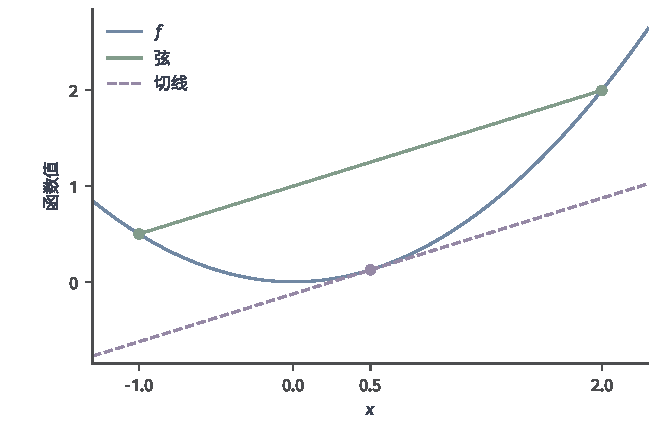
\includegraphics[width=112.0mm]{figures/01-mathematical-preliminaries-upper/01-mathematical-language-combinatorics-analysis-optimization/matplotlib/opt-convex-chord-tangent/figure.pdf}
  \caption{$f(x)=x^2/2$的弦与切线。蓝线为函数，绿线连接$u=-1$与$v=2$的函数值，
 在这两个输入之间给出弦上界；紫虚线是在$x_0=1/2$处的一阶仿射下界，适用于整个实线。
 绿线的上界只在其端点之间使用，切线下界来自凸性。图为解析教学示例。}
 \label{fig:opt-convex-chord-tangent}
\end{figure}

对扩展实值目标，式~\eqref{eq:opt-convex-function}在有限取值的点上检验，
并要求有效定义域凸；这避免在端点权重为零时操作$0\cdot(+\infty)$。

\subsubsection{严格凸性与解的唯一性}

凸函数可以沿某个方向保持不变，局部到全局的保证并没有排除多个最小点。
最小点不唯一会影响两件事：返回哪一个解取决于算法细节而不是问题本身，与最小点距离
有关的误差界也无从定义。若希望排除这种平坦的最优线段，需要把不同点之间的凸性不等式
加强为严格不等式。
\begin{definition}[严格凸函数]
\label{def:opt-strict-convexity}
设$C$凸，$f:C\to\mathbb R$。若式~\eqref{eq:opt-convex-function}对所有
$\bm u\neq\bm v$及$0<\theta<1$严格成立，则称$f$严格凸。
\end{definition}
若两个不同点$\bm u,\bm v$都达到最小值$m$，严格凸性使其中点的函数值严格小于
$(m+m)/2=m$，矛盾。因此它只保证至多一个最小点；严格凸函数$e^x$在实线上仍没有最小点。
存在性必须另由前一小节的条件检验。
在式~\eqref{eq:opt-regularized-least-squares}中，$\lambda=0$且$\bm X$不满列秩时沿零空间
方向目标不变；$\bm X$满列秩或$\lambda>0$时，任意非零方向$\bm d$都有
$\|\bm X\bm d\|_2^2/n+\lambda\|\bm d\|_2^2>0$，故目标严格凸。
与闭可行域上的存在性合用，才能断言有唯一解。

\subsubsection{强凸性与误差控制}

严格凸保证最小点至多一个，却不给统一曲率下界：两个严格凸函数可以一个像浅口碗、一个像
深漏斗，而严格凸的定义只要求“中点严格更低”，没有规定低多少。这个“低多少”直接决定
从目标误差能换回多小的参数误差，也决定梯度类算法收敛得快慢。强凸性则要求弦段与函数之间至少留出一个与距离平方成比例的间隔。
这个定义可以用于非光滑正则项，也可以使用欧氏范数以外的范数。

\begin{definition}[相对于范数的强凸性]
\label{def:opt-strong-convexity}
设$C$是实赋范空间中的凸集，$f:C\to\mathbb{R}$，$\mu>0$。若对任意
$\bm{u},\bm{v}\in C$和$\theta\in[0,1]$都有
\begin{equation}
 f(\theta\bm{u}+(1-\theta)\bm{v})
 \leq\theta f(\bm{u})+(1-\theta)f(\bm{v})
 -\frac{\mu}{2}\theta(1-\theta)\lVert\bm{u}-\bm{v}\rVert^2,
 \label{eq:opt-norm-strong-convexity}
\end{equation}
则称$f$相对于$\lVert\cdot\rVert$是\term{$\mu$强凸}（$\mu$-strongly convex）的。
\end{definition}

在欧氏空间的开凸集上，若$f$可微，强凸性等价于一阶下界
\begin{equation}
  f(\bm{v})\geq f(\bm{u})+
  \langle\nabla f(\bm{u}),\bm{v}-\bm{u}\rangle
  +\frac{\mu}{2}\lVert\bm{v}-\bm{u}\rVert_2^2.
  \label{eq:opt-first-order-strong-convexity}
\end{equation}
可用定理~\ref{thm:opt-convexity-criteria}对
$f(\bm{w})-\mu\lVert\bm{w}\rVert_2^2/2$应用凸性判据得到这一等价关系；若$f$二阶可微，
它又等价于$\nabla^2f(\bm{w})\succeq\mu\bm{I}$。一般范数的平方未必是欧氏二次型，
因此不能把这一Hessian写法直接当作所有范数下的定义。
例如$|x|+\mu x^2/2$虽在$0$处不可微，仍相对于绝对值范数$\mu$强凸：绝对值部分满足
凸性，二次部分恰好提供式~\eqref{eq:opt-norm-strong-convexity}中的距离平方间隔。

强凸性还能把目标差转成参数距离。设$f$在凸集$C$上$\mu$强凸，且最小点$\bm w^\star$存在。
把定义用于$\bm w^\star$与任意$\bm w\in C$，并用最优性给线段上的函数值加下界，得到
\[
 f(\bm w^\star)\leq(1-t)f(\bm w^\star)+tf(\bm w)
 -\frac{\mu}{2}t(1-t)\|\bm w-\bm w^\star\|^2.
\]
除以$t>0$再令$t\downarrow0$，可得
\begin{equation}
 f(\bm w)-f(\bm w^\star)\geq\frac{\mu}{2}\|\bm w-\bm w^\star\|^2,
 \qquad
 \|\bm w-\bm w^\star\|\leq\sqrt{\frac{2(f(\bm w)-f^\star)}{\mu}}.
 \label{eq:opt-strong-convex-distance}
\end{equation}
证明并未假设最优点在内部，因此也适用于固定凸域上的非光滑目标。

抗扰动结论必须明确扰动对象。现在使用欧氏范数，固定同一个凸集$C$，只改变线性项：
$f_{\bm b}(\bm w)=f(\bm w)-\langle\bm b,\bm w\rangle$。
设$\bm w_{\bm b}$与$\bm w_{\bm c}$分别达到这两个强凸问题的最小值。
把式~\eqref{eq:opt-strong-convex-distance}分别用于两个目标后相加，得
\[
 \mu\|\bm w_{\bm b}-\bm w_{\bm c}\|_2^2
 \leq\langle\bm b-\bm c,\bm w_{\bm b}-\bm w_{\bm c}\rangle,
 \qquad
 \|\bm w_{\bm b}-\bm w_{\bm c}\|_2\leq\frac{\|\bm b-\bm c\|_2}{\mu}.
\]
这里没有改变可行域，也没有任意改变目标的曲率。约束边界变化造成的活跃集切换，
不能由这个线性扰动界一并处理。

式~\eqref{eq:opt-regularized-least-squares}的Hessian矩阵为
$\bm{X}^{\top}\bm{X}/n+\lambda\bm{I}$。当$\lambda>0$时，正则项把所有缺失曲率的
方向至少抬高到$\lambda$，因而目标$\lambda$强凸。若$\lambda=0$且$\bm{X}$不满列秩，
驻点仍是全局最优点，但解不唯一；若目标再加入非凸项，驻点甚至不再保证局部最小。

前述零空间退化满足$F(\bm w+t\bm v)=F(\bm w)$，说明曲率缺失可以产生多个解。
即使曲率处处为正且解唯一，数值问题也可能非常敏感。例如令$0<\epsilon\ll1$并考虑
\[
  f_b(w_1,w_2)=\frac12(\epsilon w_1^2+w_2^2)-bw_1.
\]
它对每个$b$都有唯一最小点$(b/\epsilon,0)$，但$b$改变$\Delta b$会使第一坐标改变
$\Delta b/\epsilon$。它是一般二次目标$\frac12\bm w^\top\bm H\bm w-\bm g^\top\bm w$在
$\bm H=\operatorname{diag}(\epsilon,1)$、$\bm g=(b,0)^\top$时的特例；拟合目标
式~\eqref{eq:opt-regularized-least-squares}去掉常数$\lVert\bm y\rVert_2^2/(2n)$后也有这种形式，其中
\[
  \bm{H}=\frac{1}{n}\bm{X}^{\top}\bm{X}+\lambda\bm{I},\qquad
  \bm g=\frac1n\bm X^\top\bm y.
\]
在对角例中，每个坐标方向都只被$\bm H$乘上一个曲率数。
对一般实对称$\bm H$，这里需要的结构结论是：可以选取$d$个单位正交方向
$\bm v_i$，使$\bm H\bm v_i=\lambda_i\bm v_i$，并使每个向量都能唯一写成
$\sum_i a_i\bm v_i$。这些方向和缩放数分别称为特征向量与特征值；
实对称矩阵的这种正交展开将在第~\ref{chap:linear-algebra-and-matrix-analysis}章证明。
若$\bm H\succ\bm0$，则
$\lambda_i=\bm v_i^\top\bm H\bm v_i>0$；记其中最小、最大者为
$\lambda_{\min}(\bm H)$、$\lambda_{\max}(\bm H)$。
展开涵盖全部方向，所以$\bm H^{-1}$在每个方向除以$\lambda_i$后，
任意向量的欧氏长度至多放大$1/\lambda_{\min}(\bm H)$倍。
当$\bm{H}\succ\bm{0}$时，最小点由$\bm H\bm w=\bm g$唯一确定；若线性项受到加性扰动
$\delta\bm{g}$，解的变化$\delta\bm w=\bm H^{-1}\delta\bm g$满足
\[
  \lVert\delta\bm{w}\rVert_2
  \leq
  \frac{1}{\lambda_{\min}(\bm{H})}
  \lVert\delta\bm{g}\rVert_2.
\]
因此$1/\lambda_{\min}(\bm{H})$控制固定尺度加性扰动的绝对放大；经过目标和变量尺度
归一化后，条件数
$\kappa(\bm{H})=\lambda_{\max}(\bm{H})/\lambda_{\min}(\bm{H})$
才刻画相对病态程度。例如$\bm{H}=\epsilon\bm{I}$的条件数为$1$，但绝对扰动仍会被
放大$1/\epsilon$倍。唯一性回答“解有几个”，敏感性还取决于所采用的扰动尺度，
不能只由唯一性或条件数笼统判断。

\section{无约束光滑目标的求解}
\label{sec:opt-smooth-iterative-methods}

有了可判定的最优性条件，还需构造能逐步接近它的参数序列。这里先限定目标可微且梯度光滑：
梯度下降用一阶信息保证单步改善，动量和预条件再利用迭代历史或曲率改变移动方向。
每种改进的保证都应与前节的曲率条件配对，而不能仅凭更新公式判断快慢。

这一节的所有更新都只在当前点附近使用局部信息，因此需要先回答两个问题：梯度给出的是
什么信息，以及顺着它走多远才安全。前一节的条件（光滑性、强凸性、PL）恰好为第二个问题
提供常数。各小节的差别就在于利用了哪一类信息：只有当前梯度、还利用历史方向，或者还
构造曲率矩阵。

\subsection{基于一阶信息的求解}
\label{sec:opt-first-order-methods}

一阶方法在当前候选附近计算线性变化，借此选择新的参数：梯度给出函数在该点最陡的
上升方向，以及沿每个方向的一阶变化率，但不给出这些变化率会怎样随位置改变。
一个直觉是，梯度只告诉你“站在山坡上，正前方哪边最陡”，却不告诉你坡势会在多远之后
变缓、转弯或出现另一个谷底；因此只凭梯度选方向，还必须另外决定迈多大一步。梯度下降
只用当前梯度；动量和加速还保留已有更新的信息，用来抵消陡峭方向上的来回摆动，并加快
平坦方向上的推进；两者都不要求显式构造Hessian。它们共用一阶信息，区别在于历史信息
怎样进入新的候选，以及这一点改变使步长允许取多大。

\subsubsection{基于梯度下降的求解}
\label{sec:opt-gradient-descent}

沿着负梯度走足够小的一步一定会下降：把位移写成$\bm d=-\eta\nabla f(\bm w)$并代入
一阶近似，函数值的变化约为$-\eta\lVert\nabla f(\bm w)\rVert_2^2$，是负的。
问题在于“足够小”没有一个可以事先使用的尺度：位移越大，被舍弃的高阶项影响越大，
下降保证可能失效。要把它换成可以计算的步长范围，需要控制移动后梯度会改变多少。
下面的光滑性条件为任意两点的梯度差提供统一上界。
可以用一个具体数字理解这条假设的作用：它给“每移动单位距离，梯度最多改变多少”定了一个
上限$L$，于是步长取$1/L$量级时，高阶项造成的反弹不会盖过一阶下降；没有这个$L$，
就无法给出一个任何位置都安全的固定步长。
\begin{definition}[欧氏梯度光滑性]
\label{def:opt-smoothness}
设$C\subseteq\mathbb R^d$开且凸，$f:C\to\mathbb R$可微，$L\geq0$有限。
$f$为\term{$L$光滑}（$L$-smooth），是指对任意$\bm u,\bm v\in C$，梯度满足
$\lVert\nabla f(\bm{u})-\nabla f(\bm{v})\rVert_2
\leq L\lVert\bm{u}-\bm{v}\rVert_2$。
\end{definition}
这里对梯度使用同一Lipschitz常数。强凸给下曲率，光滑给上曲率；$x^4$严格凸但
不在全实线上强凸，也不在全实线上具有有限的光滑常数。

梯度给出最陡的一阶下降方向：在一阶近似$f(\bm w)+\langle\nabla f(\bm w),\bm d\rangle$中，
要使增量最小，就应取$\bm d$与梯度方向相反，因为$\langle\nabla f,\bm d\rangle$
在固定$\lVert\bm d\rVert_2$时于$\bm d=-\lVert\bm d\rVert_2\nabla f/\lVert\nabla f\rVert_2$
取得最小值。但一步走多远取决于函数弯曲程度，一阶近似本身不能回答；光滑性把局部线性近似的
余项控制为二次量\scite{math-nocedal2006numerical}。本小节考虑可微函数
$f:\mathbb R^d\to\mathbb R$，并选取一个正的梯度Lipschitz上界$L>0$。
若梯度恒定，仍可选择任意正上界；这样后面的$1/L$步长也有定义。
全空间的设定保证更新点仍在函数定义域内；若目标只定义在开凸子域上，使用下降引理时
还须确认两端点及其线段留在该域内，不能直接把任意梯度步代入。

\begin{lemma}[下降引理]
\label{lem:opt-descent}
若$f:\mathbb R^d\to\mathbb R$可微且梯度是$L$-Lipschitz连续的，$L>0$，则对任意
$\bm u,\bm v\in\mathbb R^d$，
\begin{equation}
  f(\bm{v})\leq f(\bm{u})
  +\langle\nabla f(\bm{u}),\bm{v}-\bm{u}\rangle
  +\frac{L}{2}\lVert\bm{v}-\bm{u}\rVert_2^2.
  \label{eq:opt-descent-lemma}
\end{equation}
\end{lemma}

\begin{proof}
令$\bm{d}=\bm{v}-\bm{u}$。沿线段积分并减去一阶项可得
\[
  f(\bm{v})-f(\bm{u})-\langle\nabla f(\bm{u}),\bm{d}\rangle
  =
  \int_0^1
  \langle\nabla f(\bm{u}+t\bm{d})-\nabla f(\bm{u}),\bm{d}\rangle\,dt.
\]
由Cauchy--Schwarz不等式和梯度Lipschitz条件，被积函数至多为
$Lt\lVert\bm{d}\rVert_2^2$；积分即得结论。
\end{proof}

在当前点$\bm w$，一阶近似为$f(\bm w)+\langle\nabla f(\bm w),\bm d\rangle$。
给定步长$\eta>0$，给这条近似加上控制移动幅度的$\|\bm d\|_2^2/(2\eta)$，其唯一最小增量是
$\bm d=-\eta\nabla f(\bm w)$。由此得到梯度下降更新
\begin{equation}
  \bm{w}^{(t+1)}
  =\bm{w}^{(t)}-\eta\nabla f(\bm{w}^{(t)}).
  \label{eq:opt-gradient-descent}
\end{equation}
把更新后的点代入下降引理，得到
\begin{equation}
  f(\bm{w}^{(t+1)})
  \leq f(\bm{w}^{(t)})
  -\eta\left(1-\frac{L\eta}{2}\right)
  \lVert\nabla f(\bm{w}^{(t)})\rVert_2^2.
  \label{eq:opt-gradient-single-step}
\end{equation}
所以$0<\eta<2/L$保证每个非驻点处严格下降。若$f$下有界，记其有限下确界为
\[
  f_{\inf}:=\inf_{\bm{w}\in\mathbb{R}^d}f(\bm{w})>-\infty.
\]
取$\eta=1/L$并对$t=0,\ldots,T-1$求和，可得非凸光滑情形的保证
\begin{equation}
  \min_{0\leq t<T}\lVert\nabla f(\bm{w}^{(t)})\rVert_2^2
  \leq
  \frac{2L(f(\bm{w}^{(0)})-f_{\inf})}{T}.
  \label{eq:opt-nonconvex-gradient-rate}
\end{equation}
它只说明某次迭代接近驻点，没有声称驻点是全局最优点。

步长上界在一维二次函数上即可看到。对$f(w)=Lw^2/2$，
$w^{(t+1)}=(1-\eta L)w^{(t)}$。当$\eta=2/L$时迭代在正负之间等幅振荡；
$\eta>2/L$时幅度按$|1-\eta L|>1$增长。负梯度方向本身没有错，失败来自步长跨过了
曲率允许的稳定范围。

若$f$还凸、最小点$\bm{w}^{\star}$存在，并继续取$\eta=1/L$，则由凸性有
$f(\bm{w}^{(t)})-f^\star
\leq\langle\nabla f(\bm{w}^{(t)}),\bm{w}^{(t)}-\bm{w}^{\star}\rangle$。
先展开距离平方并使用这个不等式：
\begin{align*}
  \lVert\bm{w}^{(t+1)}-\bm{w}^{\star}\rVert_2^2
  &=
  \lVert\bm{w}^{(t)}-\bm{w}^{\star}\rVert_2^2
  -\frac{2}{L}
  \left\langle\nabla f(\bm{w}^{(t)}),
  \bm{w}^{(t)}-\bm{w}^{\star}\right\rangle\\
  &\qquad
  +\frac{1}{L^2}\lVert\nabla f(\bm{w}^{(t)})\rVert_2^2\\
  &\leq
  \lVert\bm{w}^{(t)}-\bm{w}^{\star}\rVert_2^2
  -\frac{2}{L}\bigl(f(\bm{w}^{(t)})-f^\star\bigr)\\
  &\qquad
  +\frac{1}{L^2}\lVert\nabla f(\bm{w}^{(t)})\rVert_2^2.
\end{align*}
另一方面，把$\eta=1/L$代入式~\eqref{eq:opt-gradient-single-step}可得
\[
  \frac{1}{L^2}\lVert\nabla f(\bm{w}^{(t)})\rVert_2^2
  \leq
  \frac{2}{L}\bigl(
  f(\bm{w}^{(t)})-f(\bm{w}^{(t+1)})\bigr).
\]
用后一式消去梯度平方项，得到
\[
  \lVert\bm{w}^{(t+1)}-\bm{w}^{\star}\rVert_2^2
  \leq
  \lVert\bm{w}^{(t)}-\bm{w}^{\star}\rVert_2^2
  -\frac{2}{L}\bigl(f(\bm{w}^{(t+1)})-f^\star\bigr).
\]
对$t=0,\ldots,T-1$求和并去掉末端的非负距离，便有
\[
  \frac{2}{L}\sum_{t=0}^{T-1}
  \bigl(f(\bm{w}^{(t+1)})-f^\star\bigr)
  \leq
  \lVert\bm{w}^{(0)}-\bm{w}^{\star}\rVert_2^2.
\]
式~\eqref{eq:opt-gradient-single-step}还说明目标值单调不增，因此左侧求和中的每一项
都不小于$f(\bm{w}^{(T)})-f^\star$。于是
\begin{equation}
  f(\bm{w}^{(T)})-f^\star
  \leq\frac{L\lVert\bm{w}^{(0)}-\bm{w}^{\star}\rVert_2^2}{2T}.
  \label{eq:opt-convex-gradient-rate}
\end{equation}

\term{Polyak--Łojasiewicz条件}（PL condition）不约束函数图像必须凸，而用梯度大小控制
距离最优值还有多少差距。
\begin{definition}[Polyak--Łojasiewicz条件]
\label{def:opt-pl-condition}
设$f:\mathbb{R}^d\to\mathbb{R}$可微，$f^\star=\inf_{\bm{w}}f(\bm{w})> -\infty$。
若存在$\mu>0$，使任意$\bm{w}$满足
\begin{equation}
  \frac{1}{2}\lVert\nabla f(\bm{w})\rVert_2^2
  \geq \mu\bigl(f(\bm{w})-f^{\star}\bigr),
  \qquad \mu>0.
  \label{eq:opt-pl-condition}
\end{equation}
则称$f$满足常数为$\mu$的PL条件。
\end{definition}
该条件把小梯度与小目标误差联系起来。强凸可推出PL条件：对$\mu$强凸可微函数，把强凸
下界右侧关于$\bm{v}$最小化，得到
\[
  f^\star\geq
  f(\bm{w})-\frac{1}{2\mu}\lVert\nabla f(\bm{w})\rVert_2^2,
\]
移项正是式~\eqref{eq:opt-pl-condition}。这个推导使用全局强凸下界；只有局部Hessian
正定时，不能直接得到全域PL条件。反过来，PL函数可以有多个最小点。

PL条件也确实可以出现在非凸函数中。考虑
\[
  f(x,y)=x^2+2\sin^2x.
\]
它与$y$无关，因而最小点不唯一。其一阶导数为
$\partial f/\partial x=2(x+\sin 2x)$；当$x>0$时，若$x\leq1$则两项均非负，
若$x>1$则$x+\sin2x\geq x-1>0$，负半轴由奇对称性处理，所以导数只在$x=0$时
为零。比值
\[
  R(x)=\frac{\lVert\nabla f(x,y)\rVert_2^2}{2f(x,y)}
\]
在$x\neq0$时为正，并且$x\to0$时趋于$6$，$|x|\to\infty$时趋于$2$。
把两端之外的剩余区域限制为紧集，连续函数$R$在其中有正下界，故某个$\mu>0$使
式~\eqref{eq:opt-pl-condition}成立。另一方面，
$\partial^2 f/\partial x^2=2+4\cos2x$在某些点为负，所以$f$并不凸；该二阶导数
下界为$-2$、绝对值上界为$6$，所以它仍是$6$光滑的。负曲率下界的另一用途将在
邻近方法中解释；这里的例子表明非凸性本身不排斥目标值的梯度控制。

应用PL条件时，可将已有常数减小到$0<\mu\leq L$；这不会破坏原不等式，并使下面的收缩因子非负。把式~\eqref{eq:opt-pl-condition}代入
式~\eqref{eq:opt-gradient-single-step}，在$\eta=1/L$时得到
\begin{equation}
  f(\bm{w}^{(t)})-f^\star
  \leq
  \left(1-\frac{\mu}{L}\right)^t
  \bigl(f(\bm{w}^{(0)})-f^\star\bigr).
  \label{eq:opt-pl-linear-rate}
\end{equation}
强凸函数满足PL条件，还由
$f(\bm{w})-f^\star\geq\mu\lVert\bm{w}-\bm{w}^{\star}\rVert_2^2/2$
把目标误差转成参数误差。没有强凸时，式~\eqref{eq:opt-pl-linear-rate}不保证迭代趋向
某个唯一参数。

固定步长需要已知或估计$L$，而真实问题的$L$往往只能上界估计或完全未知；估计偏大时步长过小、收敛变慢，估计偏小时下降保证失效。一种不依赖$L$具体数值的做法是先用实际函数值检验当前这一步是否真的下降了。回溯线搜索从候选步长开始缩小，直到
$f(\bm{w}-\eta\nabla f(\bm{w}))\leq
f(\bm{w})-c\eta\lVert\nabla f(\bm{w})\rVert_2^2$成立，其中$c\in(0,1)$。
学习率调度则预先或按进度改变$\eta^{(t)}$。线搜索用实际函数值核验当前一步，调度只规定时间
表；二者都不能弥补错误梯度或无下界目标。

具体执行回溯时，给定初始试探步长$\bar\eta>0$、缩减比例$\gamma\in(0,1)$与$c\in(0,1)$。
每轮先算一次$\bm g=\nabla f(\bm w)$，若$\|\bm g\|_2$已满足停止要求就返回；
否则从$\eta=\bar\eta$开始，计算候选$\bm w-\eta\bm g$的函数值，若未满足上述充分下降条件，
令$\eta\leftarrow\gamma\eta$再试，接受后进入下一轮。下降引理保证
$\eta\leq2(1-c)/L$时一定通过，所以全局$L$光滑时每轮有限次结束，
接受步长至少为$\min\{\bar\eta,2\gamma(1-c)/L\}$。
增加的成本主要是试探点函数求值，而非每次重算当前位置的梯度。

在式~\eqref{eq:opt-common-quadratic}中，$\eta=1/16$给
$\bm w^{(t)}=(2(15/16)^t,0)^\top$（$t\geq1$），于是
$f(\bm w^{(t)})=2(15/16)^{2t}$。第二坐标一步消去，第一坐标却受较大曲率限制而缓慢缩小。
$\eta=0.1$使两坐标分别乘$0.9$与$-0.6$，目标仍下降但路径振荡；
$\eta=1/8$使第二坐标等幅振荡，$\eta>1/8$使它发散。
一般非凸问题返回梯度范数最小的已访问点，式~\eqref{eq:opt-nonconvex-gradient-rate}
控制其驻点残差；凸问题可返回最后一点并用式~\eqref{eq:opt-convex-gradient-rate}控制目标差。
已知PL常数时，$\|\nabla f\|_2\leq\sqrt{2\mu\varepsilon}$足以保证目标差不超过$\varepsilon$；
不能将这条停止规则无条件用于所有光滑目标。

\subsubsection{基于动量与加速的求解}
\label{sec:opt-curvature-acceleration}

对二次函数$f(\bm{w})=\frac12\bm{w}^{\top}\bm{H}\bm{w}
-\bm{c}^{\top}\bm{w}$，设$\bm H\succ\bm 0$，则唯一最小点为$\bm w^\star=\bm H^{-1}\bm c$。
记误差$\bm e^{(t)}=\bm w^{(t)}-\bm w^\star$；由$\nabla f(\bm w)=\bm H(\bm w-\bm w^\star)$，
梯度下降的误差满足
$\bm{e}^{(t+1)}=(\bm{I}-\eta\bm{H})\bm{e}^{(t)}$。沿$\bm H$的特征方向分解，曲率为
$\lambda_i$的误差分量每步乘以$1-\eta\lambda_i$。记最大、最小曲率为
$L=\lambda_{\max}(\bm H)$、$\mu=\lambda_{\min}(\bm H)$，条件数为$\kappa=L/\mu$。
陡峭方向要求$\eta<2/L$，于是最平坦方向每步只能把误差乘以$1-\eta\mu>1-2/\kappa$；
$\kappa$很大时，同一步长必须同时照顾陡峭与平坦方向，平坦方向因而收敛缓慢。

在狭长谷底上，梯度方向在两侧之间来回摆动，真正指向谷底的方向分量却每步都很小；
想象一个小球在又陡又窄的滑槽里下滑：它大部分动能用于在两壁之间左右撞击，沿槽向谷底
前进却很慢。对梯度逐步取平均，摆动分量相消，有效方向便指向谷底。这是保留历史方向的作用。
\term{动量法}（momentum method）保存过去方向，使连续几步指向同一侧的梯度能够累积。
这里采用重球（heavy-ball）形式：
\[
  \bm{v}^{(t+1)}=\beta\bm{v}^{(t)}+\nabla f(\bm{w}^{(t)}),
  \qquad
  \bm{w}^{(t+1)}=\bm{w}^{(t)}-\eta\bm{v}^{(t+1)}.
\]
取$\bm v^{(0)}=0$，或等价地令$\bm w^{(-1)}=\bm w^{(0)}$，即可启动重球迭代。
每轮只需一次当前位置梯度、一个历史方向和向量加法；它没有计算Hessian。
消去$\bm v$可得$\bm w^{(t+1)}=\bm w^{(t)}-\eta\nabla f(\bm w^{(t)})
+\beta(\bm w^{(t)}-\bm w^{(t-1)})$，
所以对上述正定二次目标，曲率为$\lambda_i$的特征方向上的误差分量满足
\[
  e_i^{(t+1)}
  =(1+\beta-\eta\lambda_i)e_i^{(t)}-\beta e_i^{(t-1)}.
\]
梯度下降的新误差只由上一步决定，$t$步后的误差分量等于初始值乘以$(1-\eta\lambda_i)^t$；
历史项使新误差同时依赖前两步，$t$步后的乘数成为另一个关于$\eta\lambda_i$的$t$次多项式。
选择$\beta$和$\eta$就是在调整这个多项式在各曲率上的大小，二者不能各自独立地任取。
该方向的两个特征根都严格位于单位圆内，当且仅当
$-1<\beta<1$且$0<\eta\lambda_i<2(1+\beta)$。因而常用的
$0\leq\beta<1$还须配合$0<\eta<2(1+\beta)/L$，才能保证所有方向稳定。
若已知$0<\mu\leq\lambda_i\leq L$，经典重球参数
\[
  \eta=\frac{4}{(\sqrt{L}+\sqrt{\mu})^2},
  \qquad
  \beta=\left(\frac{\sqrt{L}-\sqrt{\mu}}
  {\sqrt{L}+\sqrt{\mu}}\right)^2
\]
给出这一二次模型上的代表性最坏方向速率；它不是一般非凸目标或含噪梯度下的无条件
调参规则。
稳定区间也可从特征多项式
$r^2-(1+\beta-\eta\lambda_i)r+\beta$核对：实系数二次多项式的两根在单位圆内，
等价于$|\beta|<1$、$\eta\lambda_i>0$与$2+2\beta-\eta\lambda_i>0$。
经典参数的根模至多
$q=(\sqrt L-\sqrt\mu)/(\sqrt L+\sqrt\mu)$，端点的重根会带来$tq^t$因子；
因此不能不带常数地把有限步参数误差写成$q^t$。
在共同二次例上，$\eta=4/25$、$\beta=9/25$且零初速度给出精确轨迹
\[
 w_1^{(t)}=(2+0.8t)\,0.6^t,\qquad
 w_2^{(t)}=(2+3.2t)(-0.6)^t.
\]
第一步为$(1.68,-3.12)$，目标从$34$升至$79.2864$，之后仍趋于零。
重球的稳定和渐近提速不等于逐步下降；给定有限预算时要连同启动阶段比较。

\term{Nesterov加速梯度}
（Nesterov accelerated gradient）在前瞻点计算梯度：
\[
 \bm w^{(t+1)}=\bm z^{(t)}-\frac1L\nabla f(\bm z^{(t)}),\qquad
 q^{(t+1)}=\frac{1+\sqrt{1+4(q^{(t)})^2}}2,
\]
\[
 \bm z^{(t+1)}=\bm w^{(t+1)}
 +\frac{q^{(t)}-1}{q^{(t+1)}}(\bm w^{(t+1)}-\bm w^{(t)}).
\]
初始化为$\bm z^{(0)}=\bm w^{(0)}$、$q^{(0)}=1$。必须先得到新点，再形成下一轮前瞻点；
不能把下一轮外推系数提前用于本轮。
若$f$为凸可微函数、梯度$L$-Lipschitz连续、最小点存在，并且每步使用精确梯度和
步长$1/L$，则对$T\geq1$，
\begin{equation}
 f(\bm w^{(T)})-f^\star
 \leq\frac{2L\|\bm w^{(0)}-\bm w^\star\|_2^2}{(T+1)^2}.
 \label{eq:opt-accelerated-finite-rate}
\end{equation}
同样条件下，普通梯度下降的一般保证为$O(1/T)$。
强凸时可以另取固定外推系数
$\beta=(\sqrt L-\sqrt\mu)/(\sqrt L+\sqrt\mu)$与步长$1/L$，
获得$O((1-\sqrt{\mu/L})^T)$的目标误差界；这不是重球的步长参数。
在一维二次函数$f(w)=\lambda w^2/2$上，上述一般凸加速迭代可直接核验为
\[
  w^{(t+1)}
  =\left(1-\frac{\lambda}{L}\right)
  \bigl((1+\beta^{(t)})w^{(t)}-\beta^{(t)} w^{(t-1)}\bigr).
\]
其中$t\geq1$时$\beta^{(t)}=(q^{(t-1)}-1)/q^{(t)}$，初始化时取$\beta^{(0)}=0$。
当$\lambda=L$时一步到达零点；当$\lambda\ll L$时，跨步项改变平坦方向上的二阶递推，
但系数选错仍会振荡。二次算例不能代替一般保证，下面用势函数证明一般凸情形的界：
势函数是把目标差与到最小点的距离合在一起的非负分析量，算法本身不必计算它；
只要证明它每步不增，就能由初值读出最后的误差界。
对$\bm x^+=\bm z-\nabla f(\bm z)/L$，下降引理给$f(\bm x^+)\leq f(\bm z)-\|\nabla f(\bm z)\|_2^2/(2L)$，
凸性给$f(\bm z)\leq f(\bm v)+\langle\nabla f(\bm z),\bm z-\bm v\rangle$。两式相加，
代入$\nabla f(\bm z)=L(\bm z-\bm x^+)$并配方，得到对任意$\bm v$成立的三点不等式
\[
 f(\bm x^+)-f(\bm v)
 \leq\frac L2\bigl(\|\bm v-\bm z\|_2^2-\|\bm v-\bm x^+\|_2^2\bigr).
\]
要让相邻两步的目标差与距离项相接，我们选择一个位于当前点与最小点之间的比较点。
比较点只用于证明，不是算法需要求出的点。权重取$1/q^{(t)}$，是为了在稍后乘以
$(q^{(t)})^2$时，把旧目标差的系数变成$q^{(t)}(q^{(t)}-1)$，与$q$的递推对应。
递推使$q^{(t)}\geq1$，因而下面确为凸组合：
$\bm v=(1-1/q^{(t)})\bm w^{(t)}+\bm w^\star/q^{(t)}$。
记$\Delta^{(t)}=f(\bm w^{(t)})-f^\star$，凸性给$f(\bm v)-f^\star\leq(1-1/q^{(t)})\Delta^{(t)}$。
把$\bm z=\bm z^{(t)}$、$\bm x^+=\bm w^{(t+1)}$代入三点不等式，得到
\[
 \Delta^{(t+1)}
 \leq\Bigl(1-\frac1{q^{(t)}}\Bigr)\Delta^{(t)}
 +\frac L2\bigl(\|\bm v-\bm z^{(t)}\|_2^2-\|\bm v-\bm w^{(t+1)}\|_2^2\bigr).
\]
三点不等式中的两项距离还分别涉及外推点与新迭代点。
把它们都乘以$q^{(t)}$后，可以用同一种辅助点表示相邻状态：令
$\bm u^{(t+1)}=q^{(t)}\bm w^{(t+1)}-(q^{(t)}-1)\bm w^{(t)}
=\bm w^{(t+1)}+(q^{(t)}-1)(\bm w^{(t+1)}-\bm w^{(t)})$及$\bm u^{(0)}=\bm w^{(0)}$。
它把外推位移合并进一个向量，只用于追踪误差，不增加算法所需的状态或梯度计算。
由$q^{(t)}\bm v=(q^{(t)}-1)\bm w^{(t)}+\bm w^\star$可得
$q^{(t)}(\bm v-\bm w^{(t+1)})=\bm w^\star-\bm u^{(t+1)}$；
把$\bm z^{(t)}$的外推定义展开，又有$q^{(t)}\bm z^{(t)}-(q^{(t)}-1)\bm w^{(t)}=\bm u^{(t)}$，
故$q^{(t)}(\bm v-\bm z^{(t)})=\bm w^\star-\bm u^{(t)}$。上式乘以$(q^{(t)})^2$后得到
\[
 (q^{(t)})^2\Delta^{(t+1)}+\frac L2\|\bm u^{(t+1)}-\bm w^\star\|_2^2
 \leq q^{(t)}(q^{(t)}-1)\Delta^{(t)}+\frac L2\|\bm u^{(t)}-\bm w^\star\|_2^2.
\]
将左侧记为$E^{(t+1)}$：它把加权目标差与辅助点到最小点的距离平方相加。
取$E^{(0)}=L\|\bm w^{(0)}-\bm w^\star\|_2^2/2$。
先核对启动时的两次比较。$q^{(0)}=1$使$\bm u^{(1)}=\bm w^{(1)}$，
而$q^{(1)}(q^{(1)}-1)=1$，所以
\[
\begin{aligned}
 E^{(1)}&=\Delta^{(1)}+\frac L2\|\bm w^{(1)}-\bm w^\star\|_2^2
          \leq E^{(0)},\\
 E^{(2)}&=(q^{(1)})^2\Delta^{(2)}
          +\frac L2\|\bm u^{(2)}-\bm w^\star\|_2^2
          \leq E^{(1)}.
\end{aligned}
\]
一般$t\geq1$时，同一恒等式
$q^{(t)}(q^{(t)}-1)=(q^{(t-1)})^2$
使右侧恰为$E^{(t)}$。这就是选取比较点权重和辅助点的作用：旧目标差的系数与旧距离项
一起组成上一步的势函数，而非分别估计两个互不相接的误差。
故$(q^{(T-1)})^2\Delta^{(T)}\leq L\|\bm w^{(0)}-\bm w^\star\|_2^2/2$。
递推又给$q^{(T-1)}\geq(T+1)/2$，即得式~\eqref{eq:opt-accelerated-finite-rate}。
每轮代价仍是一次梯度与几个向量操作，但目标未必单调；一般凸情形的目标收敛也没有规定
唯一参数。强凸时才可再用式~\eqref{eq:opt-strong-convex-distance}转成参数界。

\subsection{基于二阶信息的求解}
\label{sec:opt-second-order-methods}

在共同二次例子中，两坐标的曲率相差$16$倍，一个标量步长必须兼顾两个方向：步长大到够快消去平坦方向，陡峭方向就会振荡。
用一个物理类比理解二阶方法：梯度只告诉你当前往哪边倾斜，而曲率告诉你“再往前走一步，
坡面会转多少”。一阶方法用同一个步长对待所有方向，在缓坡上走得太慢、在陡坡上又容易
冲过头；若在局部模型中保留不同方向的曲率，就能分别调整位移，这是一阶方向之外的另一种计算选择。二阶方法需要取得或近似曲率矩阵，并求解相应方程；更准确的局部模型也带来额外计算成本。本节先看直接构造曲率模型的做法，再看只从梯度差近似曲率的做法，最后看不改变曲率模型、只改变度量尺度的预条件。

\subsubsection{基于牛顿与Gauss–Newton更新的求解}
\label{sec:opt-newton-gauss-newton}

前章的二阶展开把当前点附近的目标近似为关于位移$\bm p$的二次函数。曲率矩阵正定时，这个模型有唯一最小点，可以用该点的位移作为更新方向。\term{牛顿法}（Newton's method）由模型的驻点方程求出这一方向；曲率不正定时，方程解的含义需要另行核对。在当前参数$\bm w^{(t)}$处，模型为
\[
  m^{(t)}(\bm{p})
  =
  f(\bm{w}^{(t)})
  +\left\langle\nabla f(\bm{w}^{(t)}),\bm{p}\right\rangle
  +\frac12\bm{p}^{\top}\nabla^2f(\bm{w}^{(t)})\bm{p}.
\]
令$\nabla_{\bm{p}}m^{(t)}(\bm{p}^{(t)})=\bm{0}$，便得到牛顿方程
\[
  \nabla^2 f(\bm{w}^{(t)})\bm{p}^{(t)}
  =-\nabla f(\bm{w}^{(t)}),\qquad
  \bm{w}^{(t+1)}=\bm{w}^{(t)}+\alpha^{(t)}\bm{p}^{(t)}.
\]
若Hessian矩阵在最优点附近正定且Lipschitz连续，取单位步长可得到局部二次收敛。但Hessian矩阵
不定时，牛顿方向未必下降；离最优点较远时还需线搜索或信赖域。
可逆性只使方程有唯一解，正定性才使这个解成为二次模型的最小点。
实际过程是计算梯度与Hessian，求解线性方程得到$\bm p^{(t)}$，核验其下降性，再选择步长。
若Hessian不正定，可用$\nabla^2f+\delta^{(t)}\bm I\succ0$替代它；沿该方向执行充分下降线搜索，
而不是直接接受单位步长。奇异Hessian下也不能照写逆矩阵。

牛顿法的代价来自三处，都应在选用前核算：一是需要算出$d\times d$个二阶偏导数，
二是每轮要解一个线性方程，三是只能保证局部收敛。若梯度和曲率本身需要抽样估计，
这三项成本还会叠加。下面的界量化的是第三项。

局部二次速率有可量化的范围。设$\nabla f(\bm w^\star)=0$，在包含$\bm w^\star$的球内
$\nabla^2f(\bm w)\succeq m\bm I$且Hessian为$M$-Lipschitz，其中$m>0$。
对单位牛顿步，令$\bm e=\bm w-\bm w^\star$，沿线段积分梯度得
\[
 \bm e^+
 =\nabla^2f(\bm w)^{-1}\!
 \int_0^1\bigl(\nabla^2f(\bm w)-\nabla^2f(\bm w^\star+s\bm e)\bigr)\bm e\,ds,
 \quad
 \|\bm e^+\|_2\leq\frac{M}{2m}\|\bm e\|_2^2.
\]
初始误差足够小，使这个界将点留在同一球内，才可逐轮使用。
共同二次例的Hessian恒定，$M=0$，求解$\bm H\bm p=-\bm H\bm w$得到
$\bm p=-\bm w$，一步到达零点。一般稠密$d$维问题需要存储$O(d^2)$个矩阵元素，
直接分解约需$O(d^3)$运算；本例的对角结构才把这一成本降为$O(d)$。

对非线性最小二乘
$f(\bm{w})=\frac12\lVert\bm{r}(\bm{w})\rVert_2^2$，设
$\bm{r}:\mathbb{R}^d\to\mathbb{R}^m$二阶可微。记残差向量的Jacobian矩阵为
$\bm{J}(\bm{w})\in\mathbb{R}^{m\times d}$，其第$i$行为
$\bm{J}_{i,:}(\bm{w})=\nabla r_i(\bm{w})^{\top}$，则
\[
  \nabla^2f(\bm{w})
  =\bm{J}(\bm{w})^{\top}\bm{J}(\bm{w})
  +\sum_{i=1}^m r_i(\bm{w})\nabla^2r_i(\bm{w}).
\]
\term{Gauss--Newton法}忽略第二项，使用半正定矩阵
$\bm{J}^{\top}\bm{J}$。当残差小或残差函数近似线性时近似合理；残差大时，省略项可能
决定曲率。
它的方向不是凭空替换矩阵，而是先线性化残差，求解
\[
 \min_{\bm p}\frac12\|\bm r(\bm w)+\bm J(\bm w)\bm p\|_2^2,
 \qquad
 \bm J^\top\bm J\bm p=-\bm J^\top\bm r.
\]
残差Jacobian描述每个残差对参数的变化，Hessian描述整个标量目标的曲率，两者维度也不同。
$\bm J$满列秩时子问题方向唯一；秩亏时可用QR或奇异值分解取最小范数方向，
也可增加$\delta\|\bm p\|_2^2/2$得到
$(\bm J^\top\bm J+\delta\bm I)\bm p=-\bm J^\top\bm r$。
对未正则化子问题，直接形成正规方程会平方条件数，数值实现常直接解线性最小二乘。

若解附近$\bm J$满列秩且Lipschitz、残差在解处为零，则
$\bm r(\bm w)=\bm J(\bm w)(\bm w-\bm w^\star)+O(\|\bm w-\bm w^\star\|_2^2)$，
左逆一致有界便给出局部二次误差。非零残差时，把一次Gauss--Newton更新看成从当前参数到
下一步参数的迭代映射
\[
 \bm G(\bm w)=\bm w-\bigl(\bm J(\bm w)^\top\bm J(\bm w)\bigr)^{-1}\bm J(\bm w)^\top\bm r(\bm w),
 \qquad \bm w^{(t+1)}=\bm G(\bm w^{(t)}).
\]
设局部解$\bm w^\star$附近$\bm J$满列秩、各残差二阶连续可微，记$\bm J^\star=\bm J(\bm w^\star)$、
$\bm E^\star=\sum_i r_i(\bm w^\star)\nabla^2r_i(\bm w^\star)$。驻点满足
$\nabla f(\bm w^\star)=\bm J^{\star\top}\bm r(\bm w^\star)=\bm 0$。对乘积
$(\bm J^\top\bm J)^{-1}\nabla f$求导时，作用在逆矩阵上的项乘以$\nabla f(\bm w^\star)=\bm0$而消失，
只剩$(\bm J^{\star\top}\bm J^\star)^{-1}\nabla^2f(\bm w^\star)$；代入前面的Hessian分解得
\[
 \bm D\bm G(\bm w^\star)
 =\bm I-(\bm J^{\star\top}\bm J^\star)^{-1}\bigl(\bm J^{\star\top}\bm J^\star+\bm E^\star\bigr)
 =-(\bm J^{\star\top}\bm J^\star)^{-1}\bm E^\star.
\]
零残差时$\bm E^\star=\bm 0$，这个导数矩阵为零，与二次误差一致。非零残差时，若它在某个
向量范数诱导的矩阵范数下小于$1$，导数的连续性使$\bm G$在$\bm w^\star$的某个小球内成为
压缩映射，从球内出发的迭代局部线性收敛。这只是充分条件，速率通常只是线性的；
残差大或秩条件失效时不能保证收敛。共同二次例可取
$\bm r(\bm w)=(w_1,4w_2)^\top$，残差本身线性，Gauss--Newton与牛顿方向完全一致。

\subsubsection{基于拟牛顿更新的求解}
\label{sec:opt-quasi-newton}

完整Hessian可能难以获得，但走过一步后，已经知道位移与梯度变化。
\term{拟牛顿法}（quasi-Newton method）用这两份信息修正曲率模型，不显式计算Hessian矩阵。
记位移$\bm{s}^{(t)}=\bm{w}^{(t+1)}-\bm{w}^{(t)}$与梯度差
$\bm{y}^{(t)}=\nabla f(\bm{w}^{(t+1)})-\nabla f(\bm{w}^{(t)})$；位移是向量，
不同于后面线搜索中的标量步长。若$f$二阶连续可微，沿这段位移对梯度积分得
\[
 \bm y^{(t)}=\left(\int_0^1\nabla^2f(\bm w^{(t)}+\tau\bm s^{(t)})\,d\tau\right)\bm s^{(t)},
\]
对二次目标则恰有$\bm y^{(t)}=\bm H\bm s^{(t)}$。梯度差因而记录了Hessian沿刚走过方向的平均作用。
拟牛顿法要求新的近似矩阵至少复现这一观测，即满足割线条件
$\bm{B}^{(t+1)}\bm{s}^{(t)}=\bm{y}^{(t)}$。一维时它要求近似二阶导数等于导函数在两点间的
差商，也就是导函数图像上割线的斜率，名称由此而来。位移非零且$d\geq2$时，满足割线条件的对称矩阵不止一个。
若$\bm{B}^{(t)}$是当前的Hessian近似，Broyden--Fletcher--Goldfarb--Shanno（BFGS）更新
保持对称，并只用两个秩一项修正$\bm B^{(t)}$：
\begin{equation}
  \bm{B}^{(t+1)}
  =
  \bm{B}^{(t)}
  +
  \frac{\bm{y}^{(t)}(\bm{y}^{(t)})^{\top}}
       {(\bm{y}^{(t)})^{\top}\bm{s}^{(t)}}
  -
  \frac{\bm{B}^{(t)}\bm{s}^{(t)}(\bm{s}^{(t)})^{\top}\bm{B}^{(t)}}
       {(\bm{s}^{(t)})^{\top}\bm{B}^{(t)}\bm{s}^{(t)}}.
  \label{eq:opt-bfgs-update}
\end{equation}
当$\bm{B}^{(t)}\succ\bm{0}$且曲率条件
$(\bm{y}^{(t)})^{\top}\bm{s}^{(t)}>0$成立时，
式~\eqref{eq:opt-bfgs-update}保持$\bm{B}^{(t+1)}\succ\bm{0}$，相应搜索方向
$-(\bm{B}^{(t+1)})^{-1}\nabla f$才由正定性保证是下降方向。沿下降方向执行满足
Wolfe条件的线搜索可产生该正曲率内积。具体地，令
$\bm{w}^{(t+1)}=\bm{w}^{(t)}+\alpha^{(t)}\bm{p}^{(t)}$，其中
$\nabla f(\bm{w}^{(t)})^{\top}\bm{p}^{(t)}<0$。Wolfe条件要求存在
$0<c_1<c_2<1$使
\begin{equation}
\begin{aligned}
  f(\bm{w}^{(t+1)})
  &\leq
  f(\bm{w}^{(t)})
  +
  c_1\alpha^{(t)}
  \nabla f(\bm{w}^{(t)})^{\top}\bm{p}^{(t)},\\
  \nabla f(\bm{w}^{(t+1)})^{\top}\bm{p}^{(t)}
  &\geq
  c_2\nabla f(\bm{w}^{(t)})^{\top}\bm{p}^{(t)}.
\end{aligned}
\label{eq:opt-wolfe-conditions}
\end{equation}
第二行就是\term{Wolfe曲率条件}（Wolfe curvature condition）。由
$\bm{s}^{(t)}=\alpha^{(t)}\bm{p}^{(t)}$可得
\[
  (\bm{y}^{(t)})^{\top}\bm{s}^{(t)}
  \geq
  \alpha^{(t)}(c_2-1)
  \nabla f(\bm{w}^{(t)})^{\top}\bm{p}^{(t)}
  >0.
\]
非凸或梯度含噪时，上述条件可能难以满足，此时可能需要阻尼或跳过更新。

正定性的理由值得单独核验。省略轮次上标，对任意$\bm v\neq0$，
\[
 \bm v^\top\bm B^+\bm v
 =\bm v^\top\bm B\bm v
 -\frac{(\bm v^\top\bm B\bm s)^2}{\bm s^\top\bm B\bm s}
 +\frac{(\bm v^\top\bm y)^2}{\bm y^\top\bm s}.
\]
前两项由$\bm B$内积的Cauchy--Schwarz不等式非负，仅在$\bm v$与$\bm s$平行时为零；
此时$\bm y^\top\bm s>0$又使最后一项严格为正。把更新式乘$\bm s$，
还可直接检查$\bm B^+\bm s=\bm y$。割线条件只匹配一个观测方向，不等于已经恢复全部曲率。

一次BFGS迭代从正定$\bm B^{(t)}$出发，解
$\bm B^{(t)}\bm p^{(t)}=-\nabla f(\bm w^{(t)})$，进行Wolfe线搜索，计算新梯度与
$(\bm s^{(t)},\bm y^{(t)})$后再更新矩阵。仅用不断缩短步长的Armijo回溯未必满足
Wolfe第二式，因为步长太小会使方向导数几乎不变；需要括住合适步长区间再缩小区间。
若观测曲率太小，给定$\delta\in(0,1)$，可以令
\[
 \widetilde{\bm y}=\theta\bm y+(1-\theta)\bm B\bm s,\qquad
 \theta=
 \begin{cases}
 1,&\bm s^\top\bm y\geq\delta\bm s^\top\bm B\bm s,\\
 \dfrac{(1-\delta)\bm s^\top\bm B\bm s}
 {\bm s^\top\bm B\bm s-\bm s^\top\bm y},&\text{其余情形}.
 \end{cases}
\]
用$\widetilde{\bm y}$替代$\bm y$便有
$\bm s^\top\widetilde{\bm y}\geq\delta\bm s^\top\bm B\bm s>0$；
代价是割线条件改为匹配修正后的曲率。零位移或不可靠梯度差应跳过更新。

牛顿法每轮都要解一个线性方程，直接分解稠密矩阵的代价是$O(d^3)$。若维护的是逆矩阵的
近似，只需一次矩阵向量乘法就能得到方向，每轮代价降为$O(d^2)$；这正是拟牛顿法更新
逆矩阵而不是更新$\bm B$并求解的原因。为避免每轮重新分解稠密矩阵，通常维护
$\bm C=\bm B^{-1}$并用等价公式
\[
 \bm C^+=(\bm I-\rho\bm s\bm y^\top)\bm C
          (\bm I-\rho\bm y\bm s^\top)+\rho\bm s\bm s^\top,
 \qquad \rho=(\bm y^\top\bm s)^{-1}.
\]
方向是$-\bm C\nabla f$，更新与乘法各需$O(d^2)$运算和存储；
有限记忆版本只保存最近$m$对位移、梯度差，以$O(md)$代价应用近似逆。
共同二次例取$\bm B^{(0)}=\bm I$，第一方向为$(-2,-32)$，精确线搜索步长为
$257/4097$；第一步并不像牛顿步直达最小点，所得
$\bm y=\bm H\bm s$才提供沿这次位移的曲率信息。精确算术与精确线搜索下，
正定二次目标的BFGS至多$d$步终止；一般光滑目标的局部超线性结论另需强凸邻域、
连续曲率与合适线搜索，不能从保持正定性直接推出。
这里比较的是到局部解的参数误差$e_t=\|\bm w^{(t)}-\bm w^\star\|_2$。
只说明误差趋于零，不能判断需要多少轮才能达到给定精度。收敛阶就是给误差下降速度定级
的量。在未有限步终止且$e_t\to0$的情形，超线性收敛（superlinear convergence）指
$e_{t+1}/e_t\to0$，即每一步相对上一步的误差比例也趋于零。
此前牛顿法的二次收敛还给出近解处$e_{t+1}\leq Ce_t^2$的更具体上界，
因此二次收敛蕴含超线性收敛，反向却不必成立。

拟牛顿方向$-(\bm B^{(t)})^{-1}\nabla f(\bm w^{(t)})$可以看成先用正定矩阵$(\bm B^{(t)})^{-1}$
重新缩放梯度，再沿缩放后的方向移动。缩放之所以能改善收敛，是因为固定步长的收敛速度
由最大与最小曲率之比决定：两个方向的曲率相差$100$倍时，一个标量步长无法同时适配它们。
按各方向曲率倒数缩放后，新的坐标里各方向曲率彼此接近，同一个步长对每个方向都合适。
这一步缩放并不专属于拟牛顿法：无论方向来自一阶还是二阶模型，坐标尺度都会影响数值计算。
\term{预条件}（preconditioning）通过改变方向的尺度改善求解，最简单的形式固定一个正定矩阵$\bm{P}$，按
\[
  \bm{w}^{(t+1)}
  =
  \bm{w}^{(t)}-\eta\bm{P}\nabla f(\bm{w}^{(t)})
\]
更新。$\bm P=\bm I$时它就是梯度下降；$\bm P$在迭代中保持不变，不像拟牛顿矩阵那样
随观测更新，下面的分析也只针对固定$\bm P$。
这等价于在新的坐标或内积下做最陡下降。取$\bm P$的正交特征分解，其中$\bm Q$的各列为单位正交特征向量，$p_i>0$为对应的特征值：
\[
  \bm{P}
  =
  \bm{Q}\operatorname{diag}(p_1,\ldots,p_d)\bm{Q}^{\top},
\]
据此定义
\[
  \bm{P}^{1/2}
  =
  \bm{Q}\operatorname{diag}(\sqrt{p_1},\ldots,\sqrt{p_d})\bm{Q}^{\top}.
\]
这就是$\bm{P}$唯一的对称正定平方根：它满足
$\bm{P}^{1/2}\bm{P}^{1/2}=\bm{P}$，并且可逆，其逆记为$\bm{P}^{-1/2}$。
对当前正定二次目标，记
\[
  \widetilde{\bm{H}}=\bm{P}^{1/2}\bm{H}\bm{P}^{1/2},
  \qquad
  0<\widetilde{\mu}
  =\lambda_{\min}(\widetilde{\bm{H}})
  \leq\lambda_{\max}(\widetilde{\bm{H}})
  =\widetilde{L}.
\]
原坐标中的误差递推为
$\bm{e}^{(t+1)}=(\bm{I}-\eta\bm{P}\bm{H})\bm{e}^{(t)}$。令
$\widetilde{\bm{e}}^{(t)}=\bm{P}^{-1/2}\bm{e}^{(t)}$，则
\[
  \widetilde{\bm{e}}^{(t+1)}
  =
  (\bm{I}-\eta\widetilde{\bm{H}})
  \widetilde{\bm{e}}^{(t)},
  \qquad
  \bm{P}^{-1/2}
  (\bm{I}-\eta\bm{P}\bm{H})
  \bm{P}^{1/2}
  =
  \bm{I}-\eta\widetilde{\bm{H}}.
\]
右侧矩阵由可逆坐标变换$\bm{P}^{1/2}$得到，因而与原误差递推矩阵相似；相似矩阵具有
相同特征值。这里相似指$\bm B$变成$\bm S^{-1}\bm B\bm S$，其中$\bm S$可逆；
若$\bm B\bm v=\lambda\bm v$，则
$(\bm S^{-1}\bm B\bm S)(\bm S^{-1}\bm v)=\lambda\bm S^{-1}\bm v$，
故同一个缩放数在新坐标中仍然出现，反向用$\bm S$也成立。
由于$\widetilde{\bm{H}}$对称正定，迭代对任意初始误差收敛当且仅当
$0<\eta<2/\widetilde{L}$。取
$\eta=2/(\widetilde{L}+\widetilde{\mu})$时，在变换后的欧氏范数中，每步最坏收缩因子为
\[
  \frac{\widetilde{\kappa}-1}{\widetilde{\kappa}+1},
  \qquad
  \widetilde{\kappa}
  =\frac{\widetilde{L}}{\widetilde{\mu}}.
\]
因此预条件的目标不是单独让$\bm{P}$的条件数小，而是让变换后曲率
$\widetilde{\bm{H}}$的条件数接近$1$。固定$\bm{P}\succ\bm{0}$只保证定义了合法内积；
若它与$\bm{H}$不匹配，$\widetilde{\kappa}$反而可能增大。对一般二阶可微的光滑强凸
函数，需要在包含迭代点及所比较点之间线段的凸区域统一满足
$\widetilde{\mu}\bm{I}\preceq
\bm{P}^{1/2}\nabla^2f(\bm{w})\bm{P}^{1/2}
\preceq\widetilde{L}\bm{I}$，上述步长范围与线性收敛解释才相应延续；变化的预条件矩阵还需
额外控制。

动量利用历史更新，牛顿类近似当前曲率，预条件改变几何尺度；三者可能组合，却不是同一种
机制。第~\ref{chap:linear-algebra-and-matrix-analysis}章“线性空间”
将从线性方程求解的角度比较预条件对搜索空间、残差和总成本的影响；
Fisher矩阵与经验梯度二阶矩的差别则留到概率对象建立之后讨论。

\begin{example}[两个曲率方向上的预条件]
\label{ex:opt-anisotropic-preconditioning}
取$f(\bm w)=(w_1^2+16w_2^2)/2$，初值$(2,2)^{\top}$。普通梯度下降若取
$\eta=0.1$，两个坐标分别乘以$0.9$与$-0.6$，因而
$\bm w^{(t)}=(2\times0.9^t,\,2\times(-0.6)^t)^{\top}$。
第二坐标来回越过谷底，第一坐标却缓慢缩小。取
$\bm P=\operatorname{diag}(1,1/16)$及$\eta=1/2$后，
$\bm P\nabla f(\bm w)=\bm w$，两坐标每步都减半。
\end{example}

\begin{figure*}[htbp]
  \centering
  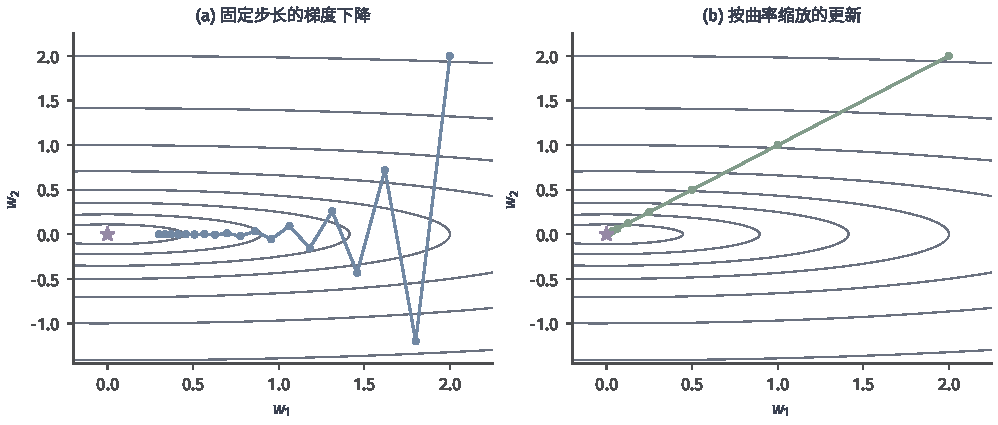
\includegraphics[width=169.0mm]{figures/01-mathematical-preliminaries-upper/01-mathematical-language-combinatorics-analysis-optimization/matplotlib/opt-preconditioned-paths/figure.pdf}
  \caption{例~\ref{ex:opt-anisotropic-preconditioning}中的精确更新路径。灰线是同一二次目标的等值线，蓝、绿圆点分别表示普通更新与预条件更新，星号是最小点。预条件使用了已知曲率，获得和应用这一矩阵的成本仍属于算法代价。}
 \label{fig:opt-preconditioned-paths}
\end{figure*}

这个例子中的预条件恰好消除了两个方向的尺度差。一般目标的曲率会随位置变化，近似矩阵
也有误差；因此图中的直达路径解释机制，不构成所有预条件方法都更快的保证。
从坐标$\bm w=\bm P^{1/2}\bm z$看，预条件只是改变测量方向长度的方式；
它也可以用于牛顿线性方程的迭代求解，并不必然是Hessian的近似逆。
在共同例中，普通$\eta=1/16$梯度法需要
$T\geq\log(2/\varepsilon)/(2\log(16/15))$（并至少一步）达到目标差$\varepsilon$；
对角预条件$\eta=1/2$的目标为$34\,4^{-T}$；
牛顿与Gauss--Newton各解一次对角系统即结束。前两者每步只做向量运算，
而一般稠密二阶方法的矩阵成本不能由这个特殊例子代表。
停止时都应核验原目标或原坐标梯度残差，而不能只看被任意缩小的预条件方向长度。
矩阵分解、条件数与线性方程残差的具体关系可回查第~\ref{chap:matrix-analysis}章。

\section{无约束非光滑目标的求解}
\label{sec:opt-nonsmooth-stochastic-methods}

绝对值损失和稀疏惩罚包含不可微点，普通梯度在那里没有定义。上一节的更新公式在尖点处
直接失去定义，不能靠减小步长绕过，因为问题出在方向本身选不出来。凸性仍能提供支撑目标的
仿射下界，允许用次梯度构造更新；若非光滑项的距离惩罚子问题容易求解，则可以保留原项，
使用邻近映射。前者的每一轮只需一个次梯度，代价低但单步可能上升；后者每轮要解一个子问题，
代价高但能利用不可微点的完整形状。两条路线需要的可计算对象不同。抽样减少信息读取量带来的误差，
在计算预算一节再讨论。

\subsection{基于次梯度的求解}
\label{sec:opt-subgradient-methods}

绝对值损失和$\ell_1$稀疏惩罚在零点不可微，因而不能直接代入普通梯度更新。
问题出在哪？以$f(x)=|x|$为例，$0$左侧的斜率是$-1$、右侧是$+1$，无论把切线斜率
取成哪一个，都只对一侧成立，不存在一个能同时描述两边的“导数”；继续套用
$x\leftarrow x-\eta f'(x)$就无从选择方向。
在可微点处，梯度等价于“过该点且处处不超过函数的唯一直线”的斜率；凸函数在不可微点处
这样的支撑直线可能不止一条。把全部支撑直线的斜率收集起来，就得到普通梯度的推广：
它不再是一个方向，而是一组方向，其中每一个都能用于比较函数值。
\begin{definition}[凸次梯度与次微分]
\label{def:opt-convex-subgradient}
设$f:\mathbb R^d\to\mathbb R\cup\{+\infty\}$为适当凸函数，$f(\bm u)$有限。
向量$\bm{g}\in\mathbb R^d$若满足
\[
  f(\bm{v})\geq f(\bm{u})+\langle\bm{g},\bm{v}-\bm{u}\rangle
  \quad\text{对所有 }\bm{v},
\]
就称为$f$在$\bm{u}$处的\term{次梯度}（subgradient）。全部次梯度组成
$\partial f(\bm{u})$，称为次微分；它可以是空集。
\end{definition}
例如
\[
  \partial |x|=
  \begin{cases}
    \{1\},&x>0,\\
    [-1,1],&x=0,\\
    \{-1\},&x<0.
  \end{cases}
\]
凸函数在$\bm{w}^{\star}$处最优，当且仅当
$\bm{0}\in\partial f(\bm{w}^{\star})$。以$f(x)=|x|$为例，零点处
$\partial f(0)=[-1,1]$，零在其中，故$0$是最小点。注意这个判据中“零向量是次梯度”
与“零向量在次微分中”是同一件事，而$\partial f$在不可微点是一整段区间，
因此“存在一个为零的次梯度”比“梯度为零”弱。
若零向量是次梯度，定义立即给出
$f(\bm{v})\geq f(\bm{w}^{\star})$；反过来，若$\bm{w}^{\star}$全局最优，则
$f(\bm{v})\geq f(\bm{w}^{\star})+\langle\bm{0},\bm{v}-\bm{w}^{\star}\rangle$，
所以零向量满足次梯度定义。这个等价性依赖凸次梯度采用全局下界定义。
若要把$f+r$的次微分直接写成$\partial f+\partial r$，或把约束写成指标函数后拆分
次微分，还需限制两个函数的定义域接触方式。
不能只凭两个函数都凸就无条件使用求和等式。本节不依赖这条求和规则，
而直接从支撑不等式推导所需的最优性关系。

次梯度迭代选$\bm g^{(t)}\in\partial f(\bm w^{(t)})$及正步长$\eta^{(t)}>0$，并令
$\bm w^{(t+1)}=\bm w^{(t)}-\eta^{(t)}\bm g^{(t)}$。
支撑斜率提供下界，却未必是实际下降方向。例如$f(x)=|x|$，在$x=0.2$取$\eta=1$，
更新到$-0.8$后目标反而增大，这一次是步长过大的结果。
尖点还可能让任意小步都不能下降：对$f(x,y)=|x|+y/2$，
在$(0,0)$可取次梯度$(1,1/2)$，沿其负方向移动$t>0$后目标为$3t/4>0$。
所以不能给次梯度更新强加光滑梯度的逐步下降要求。实际输出可取已访问点中目标最小者，
或取步长加权平均$\bar{\bm w}^{(T)}=\sum_{t<T}\eta^{(t)}\bm w^{(t)}/\sum_{t<T}\eta^{(t)}$。

用$f(x,y)=|x|+|y|$可以核对这种差别。在$(0.5,0)$处，$x$方向的支撑斜率只能为$1$，
$y$方向却可取$[-1,1]$中的任意值，因此次微分为$\{1\}\times[-1,1]$。
从中取$(1,0)^\top$，沿其负方向走到$(-0.5,0)$，函数值不变；
在$(0,0)$处可取$(1,1)^\top$，沿其负方向移动$t>0$得到目标值$2t>0$，反而上升。
这些例子排除的是逐步下降的普遍保证；后面可以对加权平均点或历史最佳点建立累计误差界，
而不是要求每个被访问点的目标值都下降。

下面在两项前提下评价误差：次梯度沿迭代有统一范数上界$G$，初值到最小点的距离不超过$R$。
设$f$凸、最小点$\bm w^\star$存在，沿迭代能取得$\|\bm g^{(t)}\|_2\leq G$，
且$\|\bm w^{(0)}-\bm w^\star\|_2\leq R$。展开距离并用次梯度下界得
\[
 \|\bm w^{(t+1)}-\bm w^\star\|_2^2
 \leq\|\bm w^{(t)}-\bm w^\star\|_2^2
 -2\eta^{(t)}(f(\bm w^{(t)})-f^\star)+(\eta^{(t)})^2G^2.
\]
求和消去中间距离，再对平均点用Jensen不等式，得到
\begin{equation}
\begin{aligned}
 \min_{t<T}(f(\bm w^{(t)})-f^\star)
 &\leq\frac{\sum_{t<T}\eta^{(t)}(f(\bm w^{(t)})-f^\star)}{\sum_{t<T}\eta^{(t)}},\\
 f(\bar{\bm w}^{(T)})-f^\star
 &\leq\frac{R^2+G^2\sum_{t<T}(\eta^{(t)})^2}{2\sum_{t<T}\eta^{(t)}}.
\end{aligned}
 \label{eq:opt-subgradient-finite-rate}
\end{equation}
同一右端也控制最佳候选。已知预算$T$且$R,G>0$时，固定
$\eta^{(t)}=R/(G\sqrt T)$给出$RG/\sqrt T$；不知道预算时可用递减步长，把实际使用的
累计步长$\sum_{t<T}\eta^{(t)}$与平方步长和$\sum_{t<T}(\eta^{(t)})^2$代入上式评价误差：
前者是加权平均的总权重，后者乘以$G^2$，给出距离递推中平方更新项的累计上界。
实际路径长度为$\sum_{t<T}\eta^{(t)}\|\bm g^{(t)}\|_2$，还依赖每次次梯度的尺度，
不能由累计步长单独确定。要使误差界趋零，总权重须相对初始距离项与平方步长项持续增大。
例如$\eta^{(t)}=R/(G\sqrt{t+1})$时，前者至少为$\sqrt T$量级，后者只按$\log T$量级增长，
误差界仍以$O(\log T/\sqrt T)$趋零。边界上次微分可能为空，强凸二次目标在全空间的次梯度也未必有界；
上界$G$必须由目标或迭代区域另行保证，不能省略。

本节的凸次梯度也不同于第~\ref{chap:mathematical-analysis}章介绍的Clarke广义梯度。
前者用一个全局仿射下界定义，直接产生凸最优性条件；后者取局部Lipschitz函数邻近可微点
梯度极限的闭凸包，允许非凸局部结构。人为指定的替代梯度更只是反向计算信号，未必属于
前面任一集合。三者名称相近，定义对象与可用结论并不相同。

\subsection{基于邻近映射的求解}
\label{sec:opt-nonsmooth-proximal}
\label{sec:opt-weaker-curvature}

次梯度法允许单步目标上升。在$|x|$的尖点，$[-1,1]$中的每个斜率都给出全局支撑线，
却不是每个负次梯度方向都能下降。换个思路：与其在许多支撑斜率里只挑一个（它未必代表尖点
两侧的全部信息），不如直接把“在尖点附近应该走到哪”当作一个小优化问题来解——
若想让更新读取尖点两侧的整个形状，
可以完整保留难处理的函数项，再加二次距离代价，限制离给定中心$\bm z$的移动。
这就把选一条支撑斜率的更新，改成在“目标小”和“离中心近”之间精确求一个折中点。
两项的作用可以分开看：只用$r$会得到可能远离当前点的最优点，只用距离项则完全不改善目标；
二次距离还带来强凸性，因而折中点总是存在且唯一。$\eta$越大越看重目标下降，越小越接近
原地不动，这正与步长的作用对应。
\begin{definition}[凸函数的邻近算子]
\label{def:opt-proximal-operator}
设$r:\mathbb R^d\to\mathbb R\cup\{+\infty\}$适当、下半连续且凸，$\eta>0$。
函数$r$的\term{邻近算子}（proximal operator）定义为
\[
  \operatorname{prox}_{\eta r}(\bm{z})
  =\argmin_{\bm{w}}
  \left\{r(\bm{w})+\frac{1}{2\eta}
  \lVert\bm{w}-\bm{z}\rVert_2^2\right\}.
\]
\end{definition}
这里的$\eta$只是算子的参数，调节$r$与距离项的相对权重；到后面的邻近点方法和近端梯度中，它才充当步长。二次项使目标强凸。
存在性还需要防止$r$下降得太快，抵消二次距离；下面直接由凸性和下半连续性证明。
后文将“适当、下半连续且凸”简称为“适当闭凸”，这里的“闭”是下半连续性的惯常表述，
不要求有效定义域本身是闭集；对偶部分将再解释这种叫法的几何含义。

\begin{proof}[邻近子问题存在与唯一]
取$\bm u\in\operatorname{dom}r$。下半连续且不取$-\infty$的$r$在紧球
$\{\bm v:\|\bm v-\bm u\|_2\leq1\}$上有有限下界$m$。
否则可取球内$r(\bm v^{(k)})\to-\infty$的序列，再取收敛子列，由下半连续性迫使极限点取$-\infty$。
对$\bm w\in\operatorname{dom}r$且$R=\|\bm w-\bm u\|_2>1$，点
$\bm v=\bm u+(\bm w-\bm u)/R$在该球上，凸性给
\[
 m\leq r(\bm v)\leq(1-1/R)r(\bm u)+r(\bm w)/R,
 \qquad
 r(\bm w)\geq r(\bm u)+R(m-r(\bm u)).
\]
所以$r$的负向增长至多线性；对固定$\bm z$，$\|\bm w-\bm z\|_2^2/(2\eta)$
支配这一线性项。邻近目标强制、下半连续且适当，由存在性小节达到最小值。
其$1/\eta$强凸性又排除两个不同最小点，因而每个$\bm z$都有唯一输出。
\end{proof}

还可以直接取得最优性关系而不预用次微分求和规则。令$\bm p$为邻近最小点，
比较它与$\bm p+t(\bm v-\bm p)$，用$r$的凸性上界并展开平方，除以$t$再令$t\downarrow0$，得
\[
 r(\bm v)\geq r(\bm p)+
 \left\langle\frac{\bm z-\bm p}{\eta},\bm v-\bm p\right\rangle.
\]
故$(\bm z-\bm p)/\eta\in\partial r(\bm p)$；反向将该下界与平方距离相加又可证明最优。
这个关系同时给出邻近解的核验条件。

\begin{theorem}[$\ell_1$邻近算子是软阈值]
\label{thm:opt-soft-threshold}
设$\lambda\geq0$、$\eta>0$。对$r(\bm{w})=\lambda\lVert\bm{w}\rVert_1$，
\[
  [\operatorname{prox}_{\eta r}(\bm{z})]_j
  =\operatorname{sign}(z_j)\max\{|z_j|-\eta\lambda,0\}.
\]
\end{theorem}

\begin{proof}
目标按坐标可分，只需最小化
$\lambda|w|+(w-z)^2/(2\eta)$。若$w>0$，驻点为
$w=z-\eta\lambda$，只在$z>\eta\lambda$时落在该区域；若$w<0$，驻点为
$w=z+\eta\lambda$，只在$z<-\eta\lambda$时有效。若
$|z|\leq\eta\lambda$，零点最优性条件
$0\in\lambda[-1,1]-z/\eta$成立，所以$w=0$。合并三种情形即得结论。
\end{proof}

例如取$\bm z=(3,0.4,-2)^{\top}$与$\eta\lambda=1$，软阈值输出
$(2,0,-1)^{\top}$；小幅坐标被直接置零。若改用
$r(\bm w)=\lambda\lVert\bm w\rVert_2^2/2$，逐坐标驻点给出
$\operatorname{prox}_{\eta r}(\bm z)=\bm z/(1+\eta\lambda)$，在同一参数下为
$(1.5,0.2,-1)^{\top}$。两种正则化都缩小幅度，只有前者在这个例子中产生精确零值。
软阈值中的零区间来自尖点处的一整段可选支撑斜率：当$|z|\leq\eta\lambda$时，
距离项要求的斜率$z/\eta$落在$\lambda[-1,1]$中，零点便能满足子问题最优性条件。
因此，产生精确零值依靠的是完整子问题的平衡，不是给原点任取一个次梯度再走一步。

邻近算子不会放大输入距离。令
$\bm{p}=\operatorname{prox}_{\eta r}(\bm{x})$、
$\bm{q}=\operatorname{prox}_{\eta r}(\bm{y})$。最优性条件给出
$(\bm{x}-\bm{p})/\eta\in\partial r(\bm{p})$和
$(\bm{y}-\bm{q})/\eta\in\partial r(\bm{q})$。把两个次梯度不等式相加，得到
\[
  \langle\bm{x}-\bm{y},\bm{p}-\bm{q}\rangle
  \geq\lVert\bm{p}-\bm{q}\rVert_2^2.
\]
再用Cauchy--Schwarz不等式便有
$\lVert\bm{p}-\bm{q}\rVert_2\leq\lVert\bm{x}-\bm{y}\rVert_2$。
这个非扩张性质依赖凸次梯度的单调性；非凸邻近子问题可能多解，不能直接沿用。

若能直接求整个目标的邻近解，邻近点方法令
$\bm w^{(t+1)}=\operatorname{prox}_{\eta^{(t)} F}(\bm w^{(t)})$。
与子问题候选$\bm w^{(t)}$比较可得
\[
 F(\bm w^{(t+1)})+\frac{\|\bm w^{(t+1)}-\bm w^{(t)}\|_2^2}{2\eta^{(t)}}
 \leq F(\bm w^{(t)}).
\]
若$F$适当闭凸且有最小点，邻近最优性关系与次梯度下界进一步给出
\[
 2\eta^{(t)}(F(\bm w^{(t+1)})-F^\star)
 \leq\|\bm w^{(t)}-\bm w^\star\|_2^2
 -\|\bm w^{(t+1)}-\bm w^\star\|_2^2
 -\|\bm w^{(t+1)}-\bm w^{(t)}\|_2^2.
\]
固定$\eta>0$时，求和并利用目标单调性得最后一点误差
$F(\bm w^{(T)})-F^\star\leq\|\bm w^{(0)}-\bm w^\star\|_2^2/(2\eta T)$。
这里没有光滑步长限制，但每一步可能需要求解一个几乎同样困难的优化问题；
数学上唯一可解不等于计算上廉价。

对$F=f+r$，若$f$可微且$L$光滑（$L>0$）、$r$适当闭凸，给定步长$\eta>0$，
近端梯度只线性化$f$，将$r$留在子问题中：
\begin{equation}
 \bm w^{(t+1)}
 =\operatorname{prox}_{\eta r}
   \bigl(\bm w^{(t)}-\eta\nabla f(\bm w^{(t)})\bigr).
 \label{eq:opt-proximal-gradient-update}
\end{equation}
一次更新依次计算$\nabla f$、形成邻近中心、求$r$的邻近解，再评价原目标。
例如共同二次目标加$r(\bm w)=\lambda\|\bm w\|_1$时，取$\eta=1/16$，
从$(2,2)$出发先到$(15/8,0)$，随后软阈值得
$(\max\{15/8-\lambda/16,0\},0)$，无需迭代求解邻近子问题。

令$\bm w^+$为该更新、$\bm d=\bm w^+-\bm w$。
邻近最优性给$-\nabla f(\bm w)-\bm d/\eta\in\partial r(\bm w^+)$，
将次梯度不等式用于旧点，再与$f$的光滑上界相加：
\begin{equation}
 F(\bm w^+)\leq F(\bm w)
 -\left(\frac1\eta-\frac L2\right)\|\bm d\|_2^2.
 \label{eq:opt-proximal-gradient-descent}
\end{equation}
故$0<\eta\leq1/L$保证下降。定义可计算的近端梯度映射
\[
 \bm G_\eta(\bm w)=\frac{\bm w-\bm w^+}{\eta}.
\]
它为零当且仅当$0\in\nabla f(\bm w)+\partial r(\bm w)$。
而$\bm G_\eta(\bm w)+\nabla f(\bm w^+)-\nabla f(\bm w)$
属于$\nabla f(\bm w^+)+\partial r(\bm w^+)$，范数至多
$(1+L\eta)\|\bm G_\eta(\bm w)\|_2$，所以这个停止残差确实控制新点的驻点性。
若$F$下有界，固定$\eta\leq1/L$时
$\min_{t<T}\|\bm G_\eta(\bm w^{(t)})\|_2^2
\leq2(F(\bm w^{(0)})-F_{\inf})/(\eta T)$。
非凸$f$下这仍只是驻点保证。

若$f$也凸，任意$\bm v\in\operatorname{dom}r$满足三点不等式
\[
 F(\bm w^+)-F(\bm v)
 \leq\frac{\|\bm w-\bm v\|_2^2-\|\bm w^+-\bm v\|_2^2}{2\eta}
 -\left(\frac1{2\eta}-\frac L2\right)\|\bm w^+-\bm w\|_2^2.
\]
它来自$f$在旧点的凸下界、在新点的光滑上界及$r$在新点的次梯度下界。
取$\bm v=\bm w^\star$、$\eta\leq1/L$并求和，便得
$F(\bm w^{(T)})-F^\star\leq\|\bm w^{(0)}-\bm w^\star\|_2^2/(2\eta T)$。
未知$L$时，可回溯增大二次模型系数直到$f$在新点不超过该模型；
每次试探都需重新求邻近解，其成本应计入预算。

前面的唯一性来自给凸函数补入正二次曲率。如果原目标已经有少量负曲率，
二次距离是否仍能补足它？弱凸性就是对所需补偿量的统一限制。
\begin{definition}[欧氏空间中的弱凸性]
\label{def:opt-weak-convexity}
设$f:\mathbb{R}^d\to\mathbb{R}\cup\{+\infty\}$是适当函数，即不恒为$+\infty$，
且$\rho\geq0$。若
$\bm{w}\mapsto f(\bm{w})+\rho\lVert\bm{w}\rVert_2^2/2$是凸函数，
则称$f$是\term{$\rho$弱凸}（$\rho$-weakly convex）的。取值$+\infty$可以用来表示不可行点。
\end{definition}
若$f$在开凸定义域上二阶可微，这等价于
$\nabla^2f(\bm{w})\succeq-\rho\bm{I}$：负曲率可以存在，但有统一下界。
当$\rho>0$且$0<\eta<1/\rho$时，对任意中心$\bm{z}$，邻近子问题的目标
\[
  f(\bm{w})+\frac{1}{2\eta}\lVert\bm{w}-\bm{z}\rVert_2^2
\]
是$(1/\eta-\rho)$强凸函数；若$\rho=0$，任意$\eta>0$都具有同样的补足曲率作用。
若$f$还下半连续，把$f+\rho\|\cdot\|_2^2/2$代入本节的直接增长证明，
剩余正二次项就保证子问题强制且有唯一解。这正是弱凸性与邻近方法的联系。补入二次曲率
只让这个子问题更易控制，并没有把原函数变成凸函数；弱凸目标仍可有局部极小点和鞍点，
也不保证求得原问题的全局最优解。

例如$f(x)=\cos x$的二阶导数是$-\cos x\geq-1$，所以它是$1$弱凸的，
但仍有无穷多个局部低点。弱凸性限制谷之间最坏的负曲率，并未消除这些谷。
若在当前位置附近加上足够大的二次惩罚，邻近子问题会得到唯一解；改变当前位置后，
所解的却是另一个邻近子问题，不能据此声称原函数只有一个最小点。
前面非凸PL例$f(x,y)=x^2+2\sin^2x$的Hessian下界为$-2\bm I$，
因此它也为$2$弱凸；这只说明两项性质可以共存，不说明任意弱凸函数都满足PL条件。
弱凸邻近映射一般也不再非扩张。例如$f(x)=-\rho x^2/2$且$0<\eta\rho<1$时，
其唯一邻近解为$z/(1-\eta\rho)$，两个输入的距离被放大$1/(1-\eta\rho)$倍。

同一个低维族能显示这些性质各自控制什么。令
\[
  f_a(x_1,x_2)=\frac12(x_1+x_2)^2+\frac{a}{2}(x_1-x_2)^2.
\]
当$a>0$时函数强凸；$a=0$时它凸且满足PL条件，但整条直线$x_1+x_2=0$都是最小点；
$a<0$时函数弱凸却无下界。若限制在紧可行域上，$a<0$时仍有最小点，但驻点
$(0,0)$可能是鞍点。这个例子说明弱凸、PL和强凸不是一条简单的强弱链：弱凸限制最坏负
曲率，PL控制梯度与目标误差，强凸还控制参数距离与唯一性。

\begin{table*}[htbp]
 \centering\small
 \begin{tabularx}{\linewidth}{@{}lXX@{}}
 \toprule
 条件 & 直接控制什么 & 单凭该条件不能得到什么\\
 \midrule
 凸性 & 全部线段上的弦上界；局部最小点也是全局最小点 & 最小点存在、唯一或统一收敛速率\\
 严格凸性 & 非平凡线段上的严格不等式；最小点至多一个 & 一致正曲率下界，例如$x^4$在原点曲率为零\\
 强凸性 & 函数值相对切平面的二次增长（可微情形） & 梯度光滑性，例如$|x|+\mu x^2/2$仍有尖点\\
 弱凸性 & 最坏负曲率的统一下界 & 驻点全局最优或最小点唯一\\
 PL条件 & 梯度大小控制目标值差 & 凸性或参数解的唯一性\\
 \bottomrule
 \end{tabularx}
 \caption{曲率条件的职责比较。各行针对不同性质，不能排成一条从“弱”到“强”的完整等级。}
 \label{tab:opt-curvature-conditions}
\end{table*}

\section{有约束优化的求解}
\label{sec:opt-constraints-duality-certificates}

目标下降的一步可能违反资源约束，因而不能只比较目标值。三种做法的共同问题是“怎样在移动方向上体现约束”：投影法改变的是移动后的落点，每次更新后强制回到可行域；惩罚法改变的是比较准则，把违反量折算进目标，让不可行的点自动变差；乘子法改变的是目标函数本身的结构，为每项约束引入一个待定的系数，并在迭代中同时更新系数与变量。三种做法都要在每步与最终的报告中分别核验原始可行性与目标质量，因为它们各自只保证了
其中一项：投影解总可行但未必改善目标，惩罚解改善折算后的目标但可能不可行，乘子法的
内层解可能既不可行也不最优。下面依次比较三种做法的子问题与停止依据；它们可以结合使用，
但都不能省略这两项核验。

\subsection{基于投影的求解}
\label{sec:opt-projected-methods}

最直接的约束处理方式是不让候选离开可行域：每次沿目标下降方向走一步，若走出了可行域，
就把落点挪到域内离它最近的位置。这一步落在哪，由可行集合的形状决定，与目标无关，
因此可以事先准备。对非空闭凸集$C$，约束指标$\iota_C$适当、下半连续且凸，
其邻近子问题只在$C$内比较平方距离。因此欧氏\term{投影}（projection）
$\Pi_C(\bm{z})=\argmin_{\bm{w}\in C}\lVert\bm{w}-\bm{z}\rVert_2^2$
把一步梯度更新拉回可行域：
\[
  \bm{w}^{(t+1)}
  =\Pi_C\bigl(\bm{w}^{(t)}-\eta^{(t)}\nabla f(\bm{w}^{(t)})\bigr).
\]
这就是取$r=\iota_C$的近端梯度，前面的邻近存在与非扩张证明直接适用。下面把最近点的
几何性质单独写出，后面对分离的证明会回用它。若$C$非凸，最近点可能不存在或不唯一。

\begin{proof}[最近点的直接几何证明]
任取$\bm{x}_0\in C$并令
$R=\lVert\bm{z}-\bm{x}_0\rVert_2$。集合
\[
  C_R=C\cap\{\bm{x}:\lVert\bm{z}-\bm{x}\rVert_2\leq R\}
\]
非空、闭且有界，因而在有限维空间中紧。连续函数
$\lVert\bm{z}-\bm{x}\rVert_2^2$在$C_R$上达到最小值；球外各点到$\bm{z}$的
距离大于$R$，而$\bm{x}_0$的距离等于$R$，所以该最小点也是$C$上的最近点。
若$\bm{p}_1,\bm{p}_2$都是最近点，最近距离为$\delta$，则凸性保证其中点属于$C$，且
\[
  \left\lVert\bm{z}-\frac{\bm{p}_1+\bm{p}_2}{2}\right\rVert_2^2
  =
  \frac12\lVert\bm{z}-\bm{p}_1\rVert_2^2
  +\frac12\lVert\bm{z}-\bm{p}_2\rVert_2^2
  -\frac14\lVert\bm{p}_1-\bm{p}_2\rVert_2^2.
\]
当$\bm{p}_1\neq\bm{p}_2$时，右端严格小于$\delta^2$，与最近距离的定义矛盾，故最近点
唯一，记为$\bm{p}$。

对任意$\bm{x}\in C$，
$\bm{p}+t(\bm{x}-\bm{p})\in C$。函数
$q(t)=\lVert\bm{z}-\bm{p}-t(\bm{x}-\bm{p})\rVert_2^2$在$t=0$
处右导数非负，所以
$\langle\bm{z}-\bm{p},\bm{x}-\bm{p}\rangle\leq0$。
展开$\|\bm z-\bm x\|_2^2$即得
\begin{equation}
 \|\bm p-\bm x\|_2^2+\|\bm z-\bm p\|_2^2\leq\|\bm z-\bm x\|_2^2,
 \qquad \bm x\in C.
 \label{eq:opt-projection-distance}
\end{equation}
\end{proof}

这说明投影不增加到任何可行参照点的距离；两个投影输出间的非扩张性则回用邻近证明。
盒约束投影只需逐坐标截断，成本为$O(d)$。
若要求非负坐标之和为$1$，得到概率单纯形（probability simplex）
$\Delta=\{\bm w\in\mathbb R^d:w_j\geq0,\ \sum_jw_j=1\}$。
它的投影具有共同阈值形式
\[
 p_j=\max\{z_j-\tau,0\},\qquad
 \sum_j\max\{z_j-\tau,0\}=1.
\]
阈值同时移动全部坐标，由总和约束确定，不能像盒投影那样完全分开计算。
为核对该形式，对$p_j>0$有$z_j-p_j=\tau$，对$p_j=0$有$z_j\leq\tau$。
故对任意$\bm x\in\Delta$，
$\langle\bm z-\bm p,\bm x-\bm p\rangle
\leq\tau\sum_j(x_j-p_j)=0$；
展开平方距离便知$\bm p$确为最近点。
常用实现先排序以确定哪些坐标为正，再解总和为$1$的阈值；
一般凸集的投影则可能本身就是大型子问题。
在共同二次目标上加范围$C=[1,2]\times[0,2]$，$\eta=0.1$的第一步先到$(1.8,-1.2)$，
再投影为$(1.8,0)$。约束最小点为$(1,0)$，其普通梯度为$(1,0)$而非零；
正确停止量是
$\|\bm w-\Pi_C(\bm w-\eta\nabla f(\bm w))\|_2/\eta$。
它与原始可行性一起检查。若$f$凸且$L$光滑、最小点存在，
前节三点不等式在$\eta\leq1/L$下直接给出目标差$O(1/T)$，
无需为投影另假设普通梯度在边界消失。

图~\ref{fig:opt-proximal-comparison}对同一个标量输入$z$比较三种处理：区间投影把
超出范围的值截到边界；软阈值把小幅值置零、其余幅值减去固定量；二次惩罚则等比例
缩小所有输入。投影保持可行性，软阈值产生稀疏性，二次惩罚改变幅度，它们都可以写成
邻近算子，但输出行为和所解决的问题不同。
\begin{figure}[!htb]
  \centering
  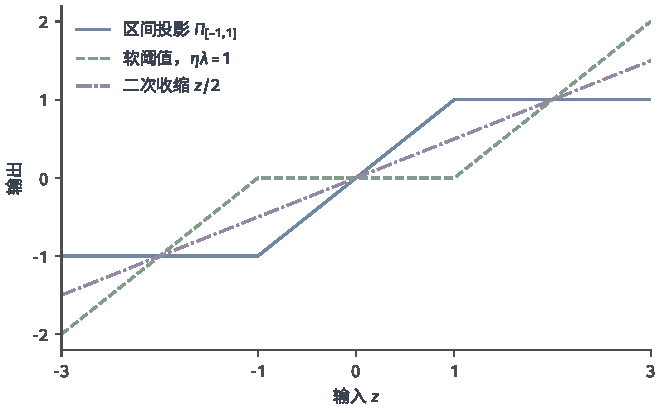
\includegraphics[width=112.0mm]{figures/01-mathematical-preliminaries-upper/01-mathematical-language-combinatorics-analysis-optimization/matplotlib/opt-proximal-comparison/figure.pdf}
  \caption{同一输入$z$的三种邻近映射。投影采用$C=[-1,1]$；软阈值与二次收缩均取$\eta\lambda=1$，分别输出$\operatorname{sign}(z)(|z|-1)_+$和$z/2$。横轴刻度标出阈值位置，曲线由完整分段解析式生成。}
 \label{fig:opt-proximal-comparison}
\end{figure}

\begin{table*}[!htb]
 \centering\small
 \begin{tabularx}{\linewidth}{@{}lXX@{}}
 \toprule
 更新方式 & 每步处理的结构 & 分析前需核对的条件\\
 \midrule
 梯度下降 & 使用可微目标的梯度 & 光滑常数与步长；全局最优保证还依赖凸性或PL等条件\\
 投影梯度 & 梯度更新后求可行集最近点 & 非空闭凸集；投影本身的计算成本\\
 次梯度更新 & 使用非光滑凸目标的全局下界斜率 & 次梯度范数及步长序列；单步目标未必下降\\
 近端梯度 & 光滑部分求梯度，非光滑部分求邻近解 & 光滑部分的步长、正则项的适当闭凸性及可解邻近子问题\\
 \bottomrule
 \end{tabularx}
 \caption{常见一阶更新的结构与条件。相近的更新形式并不共享同一收敛定理。}
 \label{tab:opt-first-order-structures}
\end{table*}

\subsection{基于惩罚的求解}
\label{sec:opt-penalty-methods}

投影可能很贵——一般凸集的投影本身就是一个优化问题；而违反约束的程度常容易计算。
于是可以换一个思路：不强制每次迭代都可行，只把违反量计入目标，让算法自己逐步远离
不可行区域。将约束写为$a_j(\bm w)=0$与$g_k(\bm w)\leq0$后，可将等式残差与不等式正部写成
$V(\bm w)=\sum_j|a_j(\bm w)|+\sum_k[g_k(\bm w)]_+$，
再最小化$f+\rho V$。$V$在约束恰好满足处一般有尖点。若$f$与各约束函数连续可微，
也可以改用平方残差构造二次惩罚$f+\frac\rho2\bigl(\sum_ja_j^2+\sum_k[g_k]_+^2\bigr)$：
$t\mapsto(t_+)^2$的导数$2t_+$连续，所以平方残差连续可微。约束仿射时，平方残差还是
梯度Lipschitz的凸函数；一般非线性约束则要另行核对光滑常数与凸性，例如$a(x)=x^2-1$
光滑，平方后的$(x^2-1)^2$却既不凸，梯度也不全局Lipschitz。
参数$\rho$越大，算法越重视可行性，但两类惩罚的有限参数性质不同。

对共同二次目标加等式$w_1+w_2=1$，二次惩罚问题为
\[
 \min_{\bm w}\frac12(w_1^2+16w_2^2)
 +\frac\rho2(w_1+w_2-1)^2.
\]
解线性驻点方程得
\[
 \bm w_\rho=\frac{(16\rho,\rho)^\top}{16+17\rho},\qquad
 w_{\rho,1}+w_{\rho,2}-1=-\frac{16}{16+17\rho}.
\]
任意有限$\rho>0$下它仍不可行，极限才是约束解$(16/17,1/17)$。
惩罚Hessian为$\operatorname{diag}(1,16)+\rho\bm 1\bm 1^\top$，特征值为
$\bigl(17+2\rho\pm\sqrt{225+4\rho^2}\bigr)/2$。最大特征值随$\rho$无限增大，
固定步长梯度法的稳定上限$2/\lambda_{\max}$因而一直缩小；最小特征值则从$1$增大并趋向$17/2$。
条件数并不单调：$\rho=0$时为$16$，$\rho=1$时约为$8.8$，在$\rho=225/34$处降到最小值约$4.9$，
此后才无限增大。小惩罚先抬高了原来最平坦方向的曲率。在单位法向$(1,1)/\sqrt2$上，
曲率为$17/2+2\rho$；在单位切向$(1,-1)/\sqrt2$上，曲率则恒为$17/2$。
不能只把增大参数看作免费提高精度。

一般可行性极限也有前提。设$P\geq0$连续且$P=0$恰好表示可行，
$f$下半连续并在候选区域有统一有限下界$m$，
$\bm w_\rho$精确最小化$f+\rho P$，并存在可行$\bar{\bm w}$。
则$\rho P(\bm w_\rho)\leq f(\bar{\bm w})-m$，所以$\rho\to\infty$时违反量趋零。
若这些解还有有界子列，其极限可行；再与任意可行点比较并使用下半连续性，可知极限全局最优。
没有有界性不能保证存在极限，近似子问题则还要将求解误差加入这个比较。

非平方的惩罚可能在有限参数精确。设比较区域$D$包含所考虑的全部候选及其可行修复，
$f$在$D$上是$K$-Lipschitz的，且每个候选$\bm w\in D$都有可行修复$\bm p\in D$满足
$\|\bm p-\bm w\|_2\leq\kappa V(\bm w)$。由于$\bm w$与$\bm p$都在$D$内，
$f(\bm w)\geq f(\bm p)-K\|\bm p-\bm w\|_2\geq f(\bm p)-K\kappa V(\bm w)$，于是
\[
 f(\bm w)+\rho V(\bm w)
 \geq f(\bm p)+(\rho-K\kappa)V(\bm w).
\]
当$\rho>K\kappa$时，$D$中任何不可行点的惩罚目标都严格大于它的修复点，
因而惩罚问题在$D$上的最优解（若存在）必须可行。
这是一条带明确误差界的精确性条件，不是所有惩罚的共同结论；
后文还将用达到的乘子给出另一种参数对应。

范数约束$\|\bm w\|_1\leq R$规定硬范围；正则项$\lambda\|\bm w\|_1$（$\lambda>0$）则按参数规模计价，
任何非零参数都要付出与其$\ell_1$范数成正比的代价，范数越大代价越高，但它
不直接强制某个预先给定的$R$。含绝对值的惩罚可调用次梯度或邻近方法；
$f$光滑且约束仿射时，二次惩罚可调用光滑方法，一般约束则先按前面的条件核对光滑性。
外层逐步提高$\rho$时，内层既要报告原目标变化，
也要报告约束违反量，不能仅凭惩罚目标的小梯度停机。

同样的区别出现在权重衰减中。普通欧氏梯度下降用于
$f(\bm{w})+\lambda\lVert\bm{w}\rVert_2^2/2$时给出
\[
  \bm{w}^{(t+1)}
  =(1-\eta\lambda)\bm{w}^{(t)}-\eta\nabla f(\bm{w}^{(t)}),
\]
与直接乘上衰减因子相同。若使用预条件矩阵$\bm{P}$，惩罚梯度产生
$-\eta\lambda\bm{P}\bm{w}^{(t)}$，而坐标无关的直接衰减仍为
$-\eta\lambda\bm{w}^{(t)}$；除非$\bm{P}=\bm{I}$或另有匹配，它们不再相同。

\subsection{基于乘子与对偶的求解}
\label{sec:opt-multiplier-dual-methods}

有限惩罚系数由任务设定，并不自动等于最优约束的影响：同一个$\rho$对不同约束的影响
可能差别很大，为了达到足够的精度往往需要反复试算。
这里先建立一个经济学直觉：在最优解处，把某条紧约束的预算放宽一点点，目标能改善多少？
这个“边际价格”不是随便拍的罚权，而是由问题自身决定的；最优解处收紧约束带来的目标增量
恰好与它挂钩。乘子就是把这一价格显式写成变量。乘子把每项约束对目标的作用写成额外
变量，让这个权重本身由问题决定：在最优点处，收紧约束带来的目标增量与乘子挂钩。
前面的惩罚法先固定一个权重再求解，乘子条件则把权重与解一起求出来。
这个平衡可以给出判据，对偶值可以给出最优值的界；要实际求解，还需规定原变量与乘子怎样更新。

\subsubsection{乘子条件与局部最优}
\label{sec:opt-kkt}

资源约束使最优点处的目标梯度不必为零，因为可行方向受到限制。考虑以下问题：
\[
  \min_{\bm{w}}f(\bm{w})
  \quad\text{s.t.}\quad
  a_j(\bm{w})=0\ (j=1,\ldots,m),\quad
  g_k(\bm{w})\leq0\ (k=1,\ldots,p)\text{。}
\]
\begin{definition}[活跃约束与线性化可行方向]
\label{def:opt-linearized-feasible-direction}
设约束函数在可行点$\bm w$处可微。不等式$g_k(\bm w)\leq0$在该点活跃，是指$g_k(\bm w)=0$。
满足
\[
  \langle\nabla a_j(\bm{w}),\bm{d}\rangle=0,\qquad
  \langle\nabla g_k(\bm{w}),\bm{d}\rangle\leq0
  \quad\text{对所有活跃的 }g_k
\]
的方向$\bm{d}$称为\term{一阶可行方向}（linearized feasible direction）。
\end{definition}
这些关系只检验约束的一阶近似，不保证$\bm w+t\bm d$在任意小的正$t$下都可行。
例如约束$x^2\leq0$在$0$处梯度为零，线性化允许任何方向，真实可行点却只有$0$；
后面的资格条件正是为了防止这种一阶信息失真。
等式约束为何产生法向量平衡，可以先看仿射情形
$\bm{A}\bm{w}=\bm{b}$。任一可行扰动都满足$\bm{A}\bm{d}=\bm{0}$；局部最优点
不能沿$\bm{d}$或$-\bm{d}$下降，故
$\langle\nabla f(\bm{w}^{\star}),\bm{d}\rangle=0$对所有
$\bm{d}\in\ker\bm{A}$成立。这里$\ker\bm A=\{\bm d:\bm A\bm d=0\}$，
矩阵乘法逐行读取内积，故$\bm A\bm d=0$恰好要求$\bm d$与每一行向量正交。
把这些行向量的全部线性组合记为$S=\{\bm A^\top\bm y:\bm y\in\mathbb R^m\}$，
就有$\ker\bm A=S^\perp$。有限维欧氏空间中，向量可分为沿子空间与垂直子空间的两部分，
因而$(S^\perp)^\perp=S$；这一正交分解的构造将在第~\ref{chap:linear-algebra-and-matrix-analysis}章给出。
其中$\operatorname{range}(\bm A^\top)$就是所有$\bm A^\top\bm y$构成的集合$S$。
于是$(\ker\bm{A})^\perp=\operatorname{range}(\bm{A}^{\top})$，存在不受符号限制的
$\bm{\nu}$使
$\nabla f(\bm{w}^{\star})=-\bm{A}^{\top}\bm{\nu}$。
这里的法向量指与所有切向可行扰动垂直的向量；$\bm A$的行给出等式面的法向量。
在共同二次目标加$w_1+w_2=1$的例子中，平衡方程为
$w_1+\nu=0$、$16w_2+\nu=0$和$w_1+w_2=1$，
解出$\nu=-16/17$、$\bm w=(16/17,1/17)^\top$。
等式乘子没有非负限制。这里的负号表示：若将规定总量从$1$稍微增加，最优目标值会增加；它不是不等式预算中的非负资源价格。后面的敏感性公式会把乘子与这一变化率联系起来。

活跃不等式只允许切平面一侧的一阶移动，它的外法向量因而以非负系数参与梯度平衡；
不活跃约束在该点留有严格余量，不限制足够小的移动，对应系数应为零。这分别引出
非负乘子与互补松弛。在适当的约束资格条件下，这些几何关系可通过
\term{拉格朗日函数}（Lagrangian）统一表达：
\[
  \mathcal{L}(\bm{w},\bm{\nu},\bm{\alpha})
  =f(\bm{w})+\sum_j\nu_j a_j(\bm{w})
  +\sum_k\alpha_k g_k(\bm{w}),
  \qquad
  \bm{\nu}\in\mathbb{R}^m,\quad
  \bm{\alpha}\in\mathbb{R}_+^p.
\]
在这里，乘子先作为未知系数，把各项约束的梯度并入驻点方程。只有在最优解、乘子与敏感性条件明确以后，才可进一步把它解释为约束变化对最优值的影响。

\begin{definition}[KKT条件]
\label{def:opt-kkt-conditions}
对于上述可微约束问题，候选点$\bm w^\star$与乘子
$\bm\nu^\star\in\mathbb R^m$、$\bm\alpha^\star\in\mathbb R^p$满足
\term{Karush--Kuhn--Tucker条件}（KKT conditions），是指以下四组关系同时成立：
\begin{align}
  \nabla_{\bm{w}}\mathcal{L}(\bm{w}^{\star},\bm{\nu}^{\star},
  \bm{\alpha}^{\star})&=\bm{0},
  &&\text{驻点性},\label{eq:opt-kkt-stationarity}\\
  a_j(\bm{w}^{\star})=0,\quad g_k(\bm{w}^{\star})&\leq0,
  &&\text{原始可行性},\\
  \alpha_k^{\star}&\geq0,
  &&\text{对偶可行性},\\
  \alpha_k^{\star}g_k(\bm{w}^{\star})&=0,
  &&\text{互补松弛}.\label{eq:opt-kkt-complementarity}
\end{align}
等式、不等式约束分别对全部$j=1,\ldots,m$与$k=1,\ldots,p$检验。
\end{definition}
互补松弛逐项连接余量与乘子：若$g_k(\bm w^\star)<0$，对应乘子必须为零；若乘子为正，对应约束必须取等号。取等号仍允许乘子为零，因此活跃约束不能反推出严格正乘子。

四组条件各自对应一条几何或经济含义。驻点性说明目标梯度被约束法向量抵消——在最优点
沿可行方向已经无法继续改善，剩余的一阶变化只能指向离开可行域的方向。原始与对偶可行性
说明候选确实可行、并且价格非负：约束变紧不该让最优值变好。互补松弛说明只有
“卡住”的约束才会标价：留有富余的约束对当前决策没有影响，价格为零；价格严格为正的
约束必然被用到边界。这四条合起来，把“局部最优”翻译成一组可以用代数核验的等式与不等式。

局部最优点满足KKT条件需要\term{约束资格条件}（constraint qualification）。
这里采用一个局部、容易核验的充分条件：$f,a_j,g_k$在点附近连续可微，
全部等式梯度与活跃不等式梯度线性无关，称为线性无关约束资格条件（LICQ）。
它与后面保证凸问题强对偶的Slater条件不是同一个假设。

可借第~\ref{chap:mathematical-analysis}章的隐函数定理直接证明LICQ下的必要性，
无需提前使用后面的分离定理。把等式值、活跃不等式值与适当补充的线性坐标组成
$\bm T(\bm w)=(\bm a(\bm w),\bm g_I(\bm w),\bm z(\bm w))$。
把这些线性无关的梯度行向量扩充为$\mathbb R^d$的一组基，再把新增行作为$\bm z(\bm w)$的系数，
就使$\bm D\bm T=[\bm D\bm a;\bm D\bm g_I;\bm D\bm z]$在当前点可逆。对$\bm T(\bm w)-\bm v=0$，以$\bm w$为待解变量、$\bm v$为参数应用隐函数定理，得到$\bm w$关于$\bm v$的局部连续可微反解，因此$\bm T$在局部给出可逆坐标变换。
未活跃不等式仍严格满足；新坐标中的可行域局部恰为
$\bm a=0,\ \bm g_I\leq0$，而$\bm z$自由。
记新坐标中的目标为$\widetilde f=f\circ\bm T^{-1}$。局部最优时，自由坐标$\bm z$的偏导为零；
活跃不等式坐标只能朝负方向移动，因此对应偏导必须非正，否则沿负方向就能降低目标。
链式法则将这些偏导还原到原坐标：
\[
 \nabla f=(\bm D\bm a)^\top\nabla_{\bm a}\widetilde f
          +(\bm D\bm g_I)^\top\nabla_{\bm g_I}\widetilde f
          +(\bm D\bm z)^\top\nabla_{\bm z}\widetilde f.
\]
最后一项为零。取$\nu_j$为等式坐标偏导的相反数、
$\alpha_k$为活跃不等式坐标偏导的相反数，再令未活跃乘子为零，
链式法则恰给$\nabla f+\sum_j\nu_j\nabla a_j+\sum_k\alpha_k\nabla g_k=0$。
非负性与互补松弛同时成立，这就建立了局部必要性。

没有资格条件，乘子可能不存在。例$f(x)=x$且约束$x^2\leq0$只有可行点
$x=0$，它当然最优；但约束梯度为零，驻点条件$1+\alpha\cdot0=0$无解。

反方向在凸情形更强。若$f$和每个$g_k$均为可微凸函数，$a_j$仿射，且某个可行点与乘子
满足KKT，则对任意可行$\bm{w}$，仿射等式约束使
$\langle\nabla a_j(\bm{w}^{\star}),\bm{w}-\bm{w}^{\star}\rangle
=a_j(\bm{w})-a_j(\bm{w}^{\star})=0$。因此等式乘子项消失，再由凸性和驻点性，
\[
  f(\bm{w})\geq
  f(\bm{w}^{\star})
  -\sum_k\alpha_k^{\star}
  \langle\nabla g_k(\bm{w}^{\star}),\bm{w}-\bm{w}^{\star}\rangle
  \geq f(\bm{w}^{\star}).
\]
最后一步使用凸约束的一阶下界、可行性和互补松弛。因此KKT在该条件下足以保证全局最优。
这个充分性证明不需要LICQ或Slater：只要确实找到满足KKT的候选即可。
反过来，非凸问题即便LICQ成立，KKT也通常只是必要条件；例如无约束$f(x)=-x^2$
在$0$满足驻点条件，却是极大点。
数值计算只能得到近似关系，宜分别报告
$\|\nabla_{\bm w}\mathcal L\|_2$、$\|\bm a\|_2$、$\|[\bm g]_+\|_2$、
$\|[-\bm\alpha]_+\|_2$及$\|\bm\alpha\odot\bm g\|_2$，
其中$\odot$表示逐坐标乘积。小残差不是无条件的目标差证书：
即使无约束凸目标$f(x)=\epsilon x^2/2$，梯度大小$\delta$也对应目标差
$\delta^2/(2\epsilon)$，仍须知道曲率尺度。若已找到精确可行点及可信的对偶下界，
才可直接用二者的差控制全局目标误差。

\begin{example}[活跃约束与乘子]
\label{ex:opt-scalar-active-constraint}
最小化$f(x)=(x-2)^2/2$，约束$x\leq a$。无约束最小点为$2$，因此
$x^\star(a)=\min\{2,a\}$。将约束写成$g(x)=x-a\leq0$，KKT条件为
$x-2+u=0$、$u\geq0$、$x\leq a$与$u(x-a)=0$。
当$a=1$时，$x^\star=1$、$u^\star=1$；当$a=3$时，$x^\star=2$、$u^\star=0$。
约束是否取等号决定乘子能否抵消目标继续下降的梯度。
最优值为$v(a)=(2-a)^2/2$对$a<2$成立，$a\geq2$时为零。
在$a=1$附近，$v'(a)=a-2=-u^\star$：增加一小单位资源上限，最优代价下降的局部速率
由乘子给出。到$a=2$时活跃集改变，解映射的导数由$1$切换为$0$；最优值仍一阶可微，两侧导数都趋于$0$。跨越切换点时，需要分别核对解导数与最优值导数。
\end{example}

\begin{example}[预算约束、活跃集与敏感性]
\label{ex:opt-kkt-budget}
求最接近$\bm{c}=(2,1)^{\top}$的非负分配，并令总预算为$\tau>0$：
\[
  \min_{\bm{w}}\frac12\lVert\bm{w}-\bm{c}\rVert_2^2
  \quad\text{s.t.}\quad
  w_1+w_2\leq\tau,\quad -w_1\leq0,\quad -w_2\leq0.
\]
当$\tau>3$时，$\bm{c}$本身严格满足预算约束，故该约束不活跃，且
$\bm{w}^{\star}(\tau)=(2,1)^{\top}$。当$\tau=3$时解仍为$\bm{c}$，预算约束活跃，
但其乘子为零；这个边界说明“约束活跃”不等于“乘子严格为正”。
当$1<\tau<3$时，两个坐标仍为正而预算取等。把预算这一不等式的乘子记为
$\alpha_{\mathrm{bud}}$，驻点条件给
\[
  w_1-2+\alpha_{\mathrm{bud}}=0,\qquad
  w_2-1+\alpha_{\mathrm{bud}}=0,\qquad
  w_1+w_2=\tau.
\]
因此
\[
  \bm{w}^{\star}(\tau)
  =\left(\frac{\tau+1}{2},\frac{\tau-1}{2}\right)^{\top},
  \qquad
  \alpha_{\mathrm{bud}}^{\star}(\tau)=\frac{3-\tau}{2}.
\]
当$0<\tau<1$时，第二个非负约束也活跃，解变成
$\bm{w}^{\star}(\tau)=(\tau,0)^{\top}$，预算乘子为$2-\tau$，第二个非负约束的
乘子为$1-\tau$。在$\tau=1$处，第二个非负约束活跃但乘子为零。上述区域及边界分别
展示预算不生效、约束活跃但零乘子、仅预算产生正价格，以及预算与坐标边界同时产生
正价格。目标严格凸，满足KKT的点都是唯一全局最优解。
\end{example}

\subsubsection{对偶下界与全局最优}
\label{sec:opt-duality}
\label{sec:opt-affine-certificates}

对固定乘子$\bm{\alpha}\geq\bm{0}$，任意可行$\bm{w}$都满足
$\mathcal{L}(\bm{w},\bm{\nu},\bm{\alpha})\leq f(\bm{w})$。因此
\term{对偶函数}（dual function）
\[
  q(\bm{\nu},\bm{\alpha})
  =\inf_{\bm{w}}\mathcal{L}(\bm{w},\bm{\nu},\bm{\alpha})
\]
给出原问题最优值的下界。我们希望在所有允许的乘子中找到最高的下界，因此定义
\[
 p^\star=\inf_{\bm w:\,\bm a(\bm w)=0,\,\bm g(\bm w)\leq0}f(\bm w),\qquad
 d^\star=\sup_{\bm\nu\in\mathbb R^m,\,\bm\alpha\geq0}q(\bm\nu,\bm\alpha).
\]
这里用下确界和上确界，不预先假定最优点或最优乘子存在。
由构造立即有$d^{\star}\leq p^{\star}$，称为\term{弱对偶}（weak duality）；
两者均有限时，差$p^{\star}-d^{\star}$称为对偶间隙。对某组乘子取下确界得到$-\infty$，表示这组
乘子没有给出有限下界；对偶不可行则表示没有任何乘子满足对偶问题规定的可行条件。前者
描述一个候选乘子的函数值，后者描述整个候选集合，二者不能混用。
若已求得原始可行$\widehat{\bm w}$与有限对偶值$q(\bm\nu,\bm\alpha)$，
则$f(\widehat{\bm w})-q(\bm\nu,\bm\alpha)$是可核验的目标差上界。
具体地，令$U=f(\widehat{\bm w})$、$L=q(\bm\nu,\bm\alpha)$，便有
$L\leq p^\star\leq U$，所以$0\leq U-p^\star\leq U-L$。
可行候选给出上界，对全部原变量取下确界的对偶值给出下界，两者的间隔才成为停止证书。
只改善对偶值还不够：求$q$时选出的内层点可能违反原约束，仍须另找可行候选形成$U$。
要说明这个间隙能否降到零，需要分析目标和约束是否能由仿射界精确描述。
下面按最近点分离、共轭重建、有限生成锥与线性规划的顺序建立这些工具；
每一步都承担不同的证明任务。

\begin{theorem}[闭凸集外一点的严格分离]
\label{thm:opt-projection-separation}
设$C\subseteq\mathbb{R}^d$非空、闭且凸，$\bm{z}\notin C$。则存在
$\bm{a}\neq\bm{0}$和$c\in\mathbb{R}$，使
\[
  \langle\bm{a},\bm{x}\rangle\leq c
  <\langle\bm{a},\bm{z}\rangle
  \quad\text{对所有 }\bm{x}\in C.
\]
\end{theorem}

\begin{proof}
由投影小节的直接证明，$\bm p=\Pi_C(\bm z)$存在且唯一，
并满足$\langle\bm z-\bm p,\bm x-\bm p\rangle\leq0$对所有$\bm x\in C$成立。
取$\bm a=\bm z-\bm p$和$c=\langle\bm a,\bm p\rangle$。由于$\bm z\notin C$，
$\bm a\neq0$，并且
$\langle\bm{a},\bm{x}\rangle\leq c$，而
$\langle\bm{a},\bm{z}\rangle=c+\lVert\bm{a}\rVert_2^2>c$。
\end{proof}

\begin{definition}[支撑超平面与凸锥]
\label{def:opt-supporting-hyperplane-cone}
设$C\subseteq\mathbb R^d$非空，$\bm a\neq0$。若$C$全部位于
$\{\bm x:\langle\bm a,\bm x\rangle\leq c\}$，并且至少有一点取等号，
则等号超平面称为$C$的\term{支撑超平面}（supporting hyperplane）。
非空集合$K$若对所有$\bm u,\bm v\in K$、$\alpha,\beta\geq0$都有
$\alpha\bm u+\beta\bm v\in K$，称为凸锥。
\end{definition}
具体地说，若$\bm{p}$位于闭凸集$C$的边界，可取一列集外点
$\bm{z}^{(k)}\to\bm{p}$，对每个点应用严格分离并把法向量归一化。单位球的紧性给出
收敛子列，极限法向量$\bm{a}\neq\bm{0}$满足
$\langle\bm{a},\bm{x}\rangle\leq\langle\bm{a},\bm{p}\rangle$对所有
$\bm{x}\in C$成立。这说明边界处至少有一个支撑方向，但边界有棱角时法向量未必唯一。
分离把“点不属于集合”转化为一个线性不等式证书，但它本身不自动给出一般凸问题的强对偶；
还需要闭性或约束资格条件。

对称矩阵集合中的\term{半正定锥}（positive semidefinite cone）
\[
  \mathbb{S}_+^d=\{\bm{M}=\bm{M}^{\top}:
  \bm{v}^{\top}\bm{M}\bm{v}\geq0,\ \forall\bm{v}\}
\]
是凸锥，因为非负线性组合仍保持二次型非负。它也是闭集：若
$\bm{M}^{(k)}\to\bm{M}$且每个$\bm{M}^{(k)}\succeq\bm{0}$，则对任意固定
$\bm{v}$都有
$\bm{v}^{\top}\bm{M}\bm{v}
=\lim_k\bm{v}^{\top}\bm{M}^{(k)}\bm{v}\geq0$。
线性规划的非负正交锥和半正定规划的矩阵约束直接定义凸可行域；标准凸二次规划中的
半正定曲率矩阵则保证目标凸。三者共享的是凸目标与凸可行域的语言。若要进一步统一成
带线性目标的锥规划，还需引入辅助变量，用锥约束表达二次目标的界。

分离用仿射函数区分一个点与可行集合。对目标函数，也可以收集所有仿射下界：
固定斜率后找最紧的截距，再比较所有斜率能否重建原函数。凸共轭承担这一步。

上图集$\operatorname{epi}f=\{(\bm x,r)\in\mathbb R^{d+1}:r\geq f(\bm x)\}$
记录图像以上的全部点；它凸与$f$凸等价，闭与$f$下半连续等价。
\begin{definition}[凸共轭与双共轭]
\label{def:opt-conjugate}
给定适当函数$f:\mathbb R^d\to\mathbb R\cup\{+\infty\}$，其\term{凸共轭}
（convex conjugate）定义为
\begin{equation}
 f^*(\bm y)=\sup_{\bm x\in\mathbb R^d}
            \{\langle\bm y,\bm x\rangle-f(\bm x)\},
 \qquad
 f^{**}(\bm x)=\sup_{\bm y\in\mathbb R^d}
            \{\langle\bm y,\bm x\rangle-f^*(\bm y)\}.
 \label{eq:opt-conjugate-biconjugate}
\end{equation}
两个上确界都在整个$\mathbb R^d$上取。$f^*$允许取$+\infty$；若$f^*\equiv+\infty$，
则$f^{**}\equiv-\infty$，否则$f^{**}$不取$-\infty$，但仍可能取$+\infty$。
\end{definition}
这里$f(\bm x)=+\infty$的点不贡献有限共轭候选。固定斜率$\bm y$时，$f^*(\bm y)$是
让$\langle\bm y,\bm x\rangle-f^*(\bm y)$在全域不超过$f$所需的最小截距修正。

\begin{example}[由斜率重建二次函数]
\label{ex:opt-quadratic-conjugate-envelope}
仍取图~\ref{fig:opt-convex-chord-tangent}中的$f(x)=x^2/2$。固定直线斜率$y$，配方得到
\[
 yx-\frac{x^2}{2}
 =\frac{y^2}{2}-\frac{(x-y)^2}{2}.
\]
右边在$x=y$时达到最大值，所以$f^*(y)=y^2/2$。这个共轭值确定了该斜率下最高的
仿射下界
\begin{equation}
 \ell_y(x)=yx-\frac{y^2}{2},\qquad
 f(x)-\ell_y(x)=\frac{(x-y)^2}{2}\geq0.
 \label{eq:opt-quadratic-affine-minorant}
\end{equation}
直线$\ell_y$在$x=y$处与抛物线相切；再提高截距，就会在该点超过$f$。
现在固定输入$x$，让斜率$y$变化。每条直线都在$f$下方，而选择$y=x$就能在这个输入
处达到$f(x)$，因此
\[
 f^{**}(x)=\sup_{y\in\mathbb R}\ell_y(x)=\frac{x^2}{2}.
\]
共轭把函数转换成“每个斜率允许多高的下界”，双共轭则在每个输入处取这些下界中最高的值。
图~\ref{fig:opt-conjugate-affine-envelope}只画三个斜率；它们的逐点最大值是折线，只有
纳入所有实数斜率，才能在每个输入处恢复这条抛物线。
\end{example}

\begin{figure}[htbp]
  \centering
  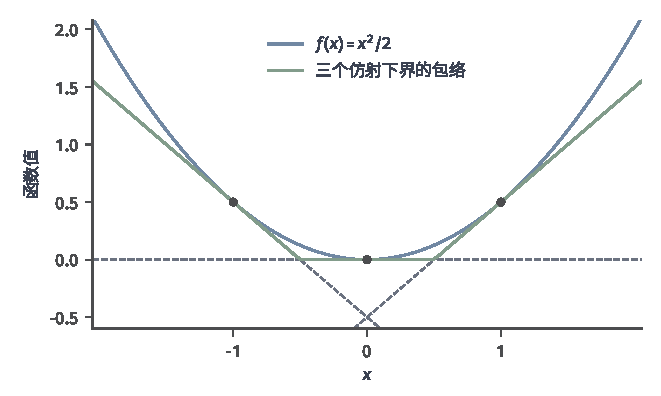
\includegraphics[width=112.0mm]{figures/01-mathematical-preliminaries-upper/01-mathematical-language-combinatorics-analysis-optimization/matplotlib/opt-conjugate-affine-envelope/figure.pdf}
  \caption{$f(x)=x^2/2$与斜率$y=-1,0,1$对应的仿射下界$\ell_y(x)=yx-y^2/2$。
 蓝实线为抛物线，三条灰虚线为下界，绿实线为这三条下界的逐点最大值。
 三个实心点标出相切位置；有限个斜率留下的间隙，在取全部斜率的上确界时消失。
 图为解析教学示例。}
 \label{fig:opt-conjugate-affine-envelope}
\end{figure}

没有任何仿射下界时，这个修正对每个斜率都为无穷。例如$f(x)=-x^2$满足
$f^*(y)=\sup_x\{yx+x^2\}=+\infty$，双共轭因而恒为$-\infty$；适当性本身不能排除这一情形。
由定义立即有\term{Fenchel--Young不等式}
\[
 f(\bm x)+f^*(\bm y)\geq\langle\bm y,\bm x\rangle,
\]
以及$f^{**}\leq f$。共轭是仿射函数族的上确界，因而凸且下半连续；它并非简单把
函数图像交换横纵坐标，也不要求每个上确界都由有限斜率达到。

\begin{theorem}[有限维Fenchel--Moreau定理]
\label{thm:opt-fenchel-moreau}
设$f:\mathbb R^d\to\mathbb R\cup\{+\infty\}$适当、下半连续且凸。
则$f^{**}=f$在全部$\mathbb R^d$上成立，包括$f(\bm x)=+\infty$的点。
因此$f$恰好是全部连续仿射下界的逐点上确界。
\end{theorem}

\begin{proof}
上图集$\operatorname{epi}f=\{(\bm x,r):r\geq f(\bm x)\}$非空、闭且凸。
任取$\bm x_0\in\operatorname{dom}f$及$t_0<f(\bm x_0)$，对上图与其外一点
$(\bm x_0,t_0)$使用定理~\ref{thm:opt-projection-separation}，得到
\[
 \langle\bm a,\bm x_0\rangle+b t_0<c
 \leq\langle\bm a,\bm z\rangle+b r
 \quad\text{对所有 }(\bm z,r)\in\operatorname{epi}f.
\]
上图沿$r$向上无界，故$b\geq0$；若$b=0$，取
$(\bm z,r)=(\bm x_0,f(\bm x_0))$便矛盾，所以$b>0$。
重排得到一个全域仿射下界$\ell_0(\bm z)=\langle\bm p_0,\bm z\rangle-\beta_0\leq f(\bm z)$。
这也保证$f^*(\bm p_0)$有限。

现任取$\bm x$和实数$t<f(\bm x)$，再次严格分离$(\bm x,t)$与上图。
若所得竖直系数$b>0$，立即得到一个仿射下界$\ell$，满足$\ell(\bm x)>t$。
若$b=0$，分离不等式为$\langle\bm a,\bm x\rangle<c\leq\langle\bm a,\bm z\rangle$。
将它与$\varepsilon(r-\ell_0(\bm z))\geq0$相加，得到
\[
 \langle\bm a-\varepsilon\bm p_0,\bm z\rangle+\varepsilon r
 \geq c-\varepsilon\beta_0.
\]
取足够小的$\varepsilon>0$，在$(\bm x,t)$处仍为严格反向不等式，因为原来的分离
间隙为正。新的竖直系数为$\varepsilon>0$，因此仍得到$\ell\leq f$且$\ell(\bm x)>t$。

将这一仿射下界写为$\ell(\bm z)=\langle\bm y,\bm z\rangle-\beta$，有
$f^*(\bm y)\leq\beta$，所以
$f^{**}(\bm x)\geq\langle\bm y,\bm x\rangle-f^*(\bm y)
\geq\ell(\bm x)>t$。
若$f(\bm x)$有限，令$t\uparrow f(\bm x)$；若$f(\bm x)=+\infty$，让$t$任意增大，
两种情形均得$f^{**}(\bm x)\geq f(\bm x)$。结合反向不等式即得结论。
\end{proof}

例~\ref{ex:opt-quadratic-conjugate-envelope}已经用切线族重建了二次函数；定理将这个结论
推广到可能不可微、允许取$+\infty$的闭凸目标。若$f=\iota_{[0,1]}$为闭区间指标函数，
则$f^*(y)=\max\{0,y\}$，双共轭恢复区间内
的零值和区间外的$+\infty$。闭性不能省略：对开区间指标$f=\iota_{(0,1)}$，共轭仍为
$\max\{0,y\}$，但双共轭成为$\iota_{[0,1]}$，在两个端点补上零值。
仿射下界无法区分一个边界点与从内部趋近的极限，下半连续性正是排除这种缺口的条件。

函数等于双共轭也不保证边界处有有限的最优斜率。例如闭凸函数
$f(x)=-\sqrt{x}$对$x\geq0$定义，负半轴取$+\infty$。在$x=0$，有限次梯度$y$若存在，
必须满足$-\sqrt{x}\geq yx$对所有$x>0$成立，即$y\leq-1/\sqrt{x}$，这是不可能的。
$f^{**}(0)=f(0)=0$仍成立，但只能由一列仿射下界逼近，不能声称共轭上确界在某个有限
$y$处达到。由双共轭推导对偶表达时，值相等与最优乘子存在必须分别证明。

共轭也能直接计算对偶下界。例如对单一等式约束问题
$\min_{\bm w}\{f(\bm w):\bm a^\top\bm w=b\}$，固定乘子$\nu$后有
\[
 q(\nu)=\inf_{\bm w}\{f(\bm w)+\nu(\bm a^\top\bm w-b)\}
       =-f^*(-\nu\bm a)-\nu b.
\]
最后一步来自把下确界取负后改写成共轭的上确界，因此不必先求出内层最小点。
若$f(\bm w)=\|\bm w\|_2^2/2$且$\bm a\neq0$，逐坐标配方给$f^*(\bm y)=\|\bm y\|_2^2/2$，
于是$q(\nu)=-\nu^2\|\bm a\|_2^2/2-\nu b$。
它在$\nu^\star=-b/\|\bm a\|_2^2$达到$b^2/(2\|\bm a\|_2^2)$；
原始可行点$\bm w^\star=b\bm a/\|\bm a\|_2^2$也取这个值，故弱对偶就足以认证双方最优。
共轭在这里计算下界，双共轭说明闭凸函数不会在收集全部仿射下界时损失函数值；
但对某个约束问题是否零间隙，仍须像这个例子一样另外核验。

接下来改用有限生成锥研究线性约束的可行性。线性规划的强对偶将由不可行证书推出，
不以双共轭等式代替证明。先建立所需的择一定理
\scite{math-boyd2004convex}

\begin{lemma}[有限生成锥的闭性]
\label{lem:opt-finitely-generated-cone}
给定$\bm{a}_1,\ldots,\bm{a}_r\in\mathbb{R}^m$，集合
\[
  K=\left\{\sum_{i=1}^r\alpha_i\bm{a}_i:\alpha_i\geq0\right\}
\]
是闭凸锥。
\end{lemma}

\begin{proof}
凸性和锥性质由非负线性组合直接得到。为证明闭性，先注意每个$\bm{x}\in K$都能由一组
线性无关的生成向量作非负组合。若某个表示使用的生成向量线性相关，就存在非零系数
$\bm{\gamma}$使$\sum_i\gamma_i\bm{a}_i=\bm{0}$；必要时改变符号，使至少一个
$\gamma_i>0$。从原系数中减去
$t\bm{\gamma}$，其中$t=\min_{\gamma_i>0}\alpha_i/\gamma_i$，仍保持所有系数
非负，并使至少一个系数变为零。重复此过程便得到线性无关的表示。

现取$\bm{x}^{(k)}\in K$且$\bm{x}^{(k)}\to\bm{x}$。线性无关的生成子集只有有限多个，
故可取子列，使每个$\bm{x}^{(k)}$都使用同一个子集$J$。以这些向量为列组成满列秩矩阵
$\bm{A}_J$，相应非负系数满足
\[
  \bm{\alpha}^{(k)}
  =(\bm{A}_J^{\top}\bm{A}_J)^{-1}\bm{A}_J^{\top}\bm{x}^{(k)}
  \longrightarrow
  (\bm{A}_J^{\top}\bm{A}_J)^{-1}\bm{A}_J^{\top}\bm{x}.
\]
极限系数仍逐项非负，且$\bm{x}$等于$\bm{A}_J$乘该极限系数，故$\bm{x}\in K$。
\end{proof}

\begin{lemma}[有限维多面体的线性像]
\label{lem:opt-polyhedral-image}
有限维多面体在线性映射下的像仍是多面体，因而是闭集。
\end{lemma}

\begin{proof}
设多面体$P=\{\bm{u}:\bm{B}\bm{u}\leq\bm{d}\}$，线性映射为
$\bm{v}=\bm{T}\bm{u}$。其图像
\[
  \{(\bm{u},\bm{v}):\bm{B}\bm{u}\leq\bm{d},\
  \bm{v}=\bm{T}\bm{u}\}
\]
是多面体，而$\bm{T}P$是该图像消去$\bm{u}$后的坐标投影。对一个待消变量，
Fourier--Motzkin消元分别收集其系数为正、为负和为零的不等式；每一对正、负系数
不等式消去该变量，零系数不等式原样保留。所得有限组非严格线性不等式恰好描述投影。
逐个消去$\bm{u}$的坐标，便得到$\bm{T}P$的有限线性不等式表示。多面体是有限个闭
半空间的交，因此闭。
\end{proof}

\begin{theorem}[Farkas择一定理]
\label{thm:opt-farkas}
给定$\bm{M}\in\mathbb{R}^{m\times d}$和$\bm{r}\in\mathbb{R}^m$，下列两个系统
恰有一个可行：
\[
  \bm{M}\bm{x}=\bm{r},\quad\bm{x}\geq\bm{0};
  \qquad
  \bm{M}^{\top}\bm{z}\geq\bm{0},\quad
  \bm{r}^{\top}\bm{z}<0.
\]
\end{theorem}

\begin{proof}
两者不能同时成立，因为若都成立，则
$0>\bm{r}^{\top}\bm{z}
=\bm{x}^{\top}\bm{M}^{\top}\bm{z}\geq0$，矛盾。
若第一个系统不可行，$\bm{r}$不属于锥
$K=\{\bm{M}\bm{x}:\bm{x}\geq\bm{0}\}$。它由$\bm{M}$的有限个列向量生成，故由
引理~\ref{lem:opt-finitely-generated-cone}可知$K$是闭凸锥。对$K$与$\bm{r}$应用
定理~\ref{thm:opt-projection-separation}，得到$\bm{a}$和$c$，使
$\langle\bm{a},\bm{k}\rangle\leq c<\langle\bm{a},\bm{r}\rangle$。
由于$\bm{0}\in K$，有$c\geq0$；又因为$t\bm{k}\in K$对所有$t\geq0$成立，
必有$\langle\bm{a},\bm{k}\rangle\leq0$，否则取充分大的$t$便会超过$c$。
令$\bm{z}=-\bm{a}$，可得$\langle\bm{z},\bm{r}\rangle<0$且
$\langle\bm{z},\bm{k}\rangle\geq0$对所有$\bm{k}\in K$成立。特别地，
对$\bm{M}$的每个列向量成立，故
$\bm{M}^{\top}\bm{z}\geq\bm{0}$。第二个系统可行。
\end{proof}

\begin{theorem}[有限维线性规划强对偶]
\label{thm:opt-lp-strong-duality}
考虑标准型原问题与对偶问题
\[
  \min_{\bm{x}\geq\bm{0}}\bm{c}^{\top}\bm{x}
  \quad\text{s.t.}\quad\bm{A}\bm{x}=\bm{b},
  \qquad
  \max_{\bm{y}}\bm{b}^{\top}\bm{y}
  \quad\text{s.t.}\quad\bm{A}^{\top}\bm{y}\leq\bm{c}.
\]
若原问题可行且有限下确界为$p^\star$，则原问题与对偶问题都有最优解，且两个最优值
都等于$p^\star$。
\end{theorem}

\begin{proof}
原始可行域
$P=\{\bm{x}:\bm{A}\bm{x}=\bm{b},\ \bm{x}\geq\bm{0}\}$是非空多面体。由
引理~\ref{lem:opt-polyhedral-image}，其目标值集合
\[
  W=\{\bm{c}^{\top}\bm{x}:\bm{x}\in P\}
\]
是$\mathbb{R}$中的非空多面体。集合$W$下有界，且一维多面体包含自己的有限下端点，
故$p^\star=\inf W$属于$W$。因此存在原始可行点$\bm{x}^{\star}$满足
$\bm{c}^{\top}\bm{x}^{\star}=p^\star$，原问题达到其最优值。

对任意$\varepsilon>0$，系统
\[
  \bm{A}\bm{x}=\bm{b},\quad
  \bm{c}^{\top}\bm{x}+s=p^\star-\varepsilon,\quad
  \bm{x}\geq\bm{0},\ s\geq0
\]
不可行，否则会有目标值小于$p^\star$的原始可行点。对增广矩阵应用
定理~\ref{thm:opt-farkas}，存在$(\bm{y}_{\varepsilon},\gamma_\varepsilon)$满足
\[
  \bm{A}^{\top}\bm{y}_{\varepsilon}
  +\gamma_\varepsilon\bm{c}\geq\bm{0},\quad
  \gamma_\varepsilon\geq0,\quad
  \bm{b}^{\top}\bm{y}_{\varepsilon}
  +\gamma_\varepsilon(p^\star-\varepsilon)<0.
\]
取任一原始可行$\bar{\bm{x}}$并与第一式作内积可知$\gamma_\varepsilon>0$，否则会与
最后一式矛盾。令
$\widehat{\bm{y}}_\varepsilon=-\bm{y}_\varepsilon/\gamma_\varepsilon$，便有
$\bm{A}^{\top}\widehat{\bm{y}}_\varepsilon\leq\bm{c}$且
$\bm{b}^{\top}\widehat{\bm{y}}_\varepsilon>p^\star-\varepsilon$。

记对偶可行多面体为
$D=\{\bm{y}:\bm{A}^{\top}\bm{y}\leq\bm{c}\}$。上面的构造说明$D$非空，且其
目标值集合
\[
  V=\{\bm{b}^{\top}\bm{y}:\bm{y}\in D\}
\]
对每个$\varepsilon>0$都包含一个大于$p^\star-\varepsilon$的值。弱对偶说明$V$中的
每个值都不超过$p^\star$，所以$\sup V=p^\star$。由
引理~\ref{lem:opt-polyhedral-image}，$V$是$\mathbb{R}$中的多面体；非空的一维
多面体只能是闭区间、闭射线、单点或整条实线。由于$V$有有限上确界，它必包含上端点
$p^\star$。因此存在$\bm{y}^{\star}\in D$使
$\bm{b}^{\top}\bm{y}^{\star}=p^\star$，对偶最优解达到与原问题相同的最优值。
\end{proof}

\begin{example}[二维资源分配的原始与对偶证书]
\label{ex:opt-resource-lp-duality}
考虑
\[
  \max_{x_1,x_2\geq0}3x_1+2x_2
  \quad\text{s.t.}\quad
  2x_1+x_2\leq4,\quad x_1+2x_2\leq4.
\]
为两类资源设置价格$u_1,u_2\geq0$。由于原问题是最大化，对可行点的资源余量按非负
价格计价会给出目标上界：
\begin{align*}
  \mathcal{L}(\bm{x},\bm{u})
  &=
  3x_1+2x_2
  +u_1(4-2x_1-x_2)+u_2(4-x_1-2x_2)\\
  &=
  4u_1+4u_2
  +(3-2u_1-u_2)x_1+(2-u_1-2u_2)x_2.
\end{align*}
要使$\sup_{\bm{x}\geq\bm{0}}\mathcal{L}(\bm{x},\bm{u})$有限，$x_1,x_2$的系数
必须非正，因而
$2u_1+u_2\geq3$且$u_1+2u_2\geq2$。此时上确界就是$4u_1+4u_2$，
最小化这个上界得到对偶
\[
  \min_{u_1,u_2\geq0}4u_1+4u_2
  \quad\text{s.t.}\quad
  2u_1+u_2\geq3,\quad u_1+2u_2\geq2.
\]
原始点$(x_1,x_2)=(4/3,4/3)$可行，值为$20/3$；对偶点
$(u_1,u_2)=(4/3,1/3)$可行，值也为$20/3$。弱对偶说明二者同时最优。两项资源约束
和两项产品约束均取等号，互补松弛也逐项成立。
\end{example}

不可行、无界和未达到必须区分。Farkas向量证明约束不可行；若原问题沿可行射线无限改善，
弱对偶只说明不存在给出有限下界的对偶候选，也就是每个允许乘子的对偶函数值都为
$-\infty$，不能据此断言乘子候选集合为空。在线性规划标准型中，这种情形表现为对偶
不可行。若只有下确界而不达到，则不能展示原始最优点。一般凸问题在使用Slater条件前还需
处理低维定义域。沿用定义~\ref{def:opt-proper-domain-indicator}的有效定义域，还需说明低维集合中的“内部”。
\begin{definition}[仿射包与相对内部]
\label{def:opt-affine-hull-relative-interior}
对非空集合$C\subseteq\mathbb R^d$，其\term{仿射包}（affine hull）是全部有限仿射组合
$\sum_i\alpha_i\bm x_i$组成的集合，其中$\bm x_i\in C$、$\sum_i\alpha_i=1$，权重可为负。
点$\bm x\in C$属于\term{相对内部}（relative interior），是指存在$r>0$使
$B(\bm x,r)\cap\operatorname{aff}C\subseteq C$。
\end{definition}

例如平面中的线段没有二维内部，但去掉两个端点后就是它的相对内部。

严格可行点提供了一个不会立即碰到不等式边界的比较位置。下面引用Slater定理的一种有限维版本，
用它判断对偶下界能否达到原最优值。
\begin{theorem}[Slater条件下的强对偶]
设$f$和不等式函数$g_k$都是适当凸函数，即它们不恒为
$+\infty$、从不取$-\infty$且至少在一点取有限值；这些函数具有共同凸定义域$D$，
等式约束为仿射约束$\bm{A}\bm{w}=\bm{b}$。若存在
\[
  \bar{\bm{w}}\in\operatorname{ri}D,\qquad
  \bm{A}\bar{\bm{w}}=\bm{b},\qquad
  g_k(\bar{\bm{w}})<0\quad\text{对所有 }k,
\]
并且原问题最优值有限，则原、对偶最优值相等，且存在最优对偶乘子。
\end{theorem}
共同定义域$D$是这些函数都取有限值的区域。相对内部允许$D$落在低维仿射空间中；
严格不等式要求在这个空间内仍有可行余量。这个条件保证存在有限乘子，足以把最优下界抬到原最优值，
但不保证原始最小点存在。其一般证明需要凸集的一般分离结论，并处理约束值与目标值组成集合的边界；
这类集合未必闭，不能直接套用前面仅针对闭凸集外一点的严格分离定理。
本章不展开这一证明，后面使用时逐项核对这里列出的共同定义域、仿射等式、严格可行点及有限最优值。价值函数与占用度量中的对偶应用
可参考\BookChapterRef{chap:decision-theory-and-dynamic-risk}{卷2《数学准备：概率、因果与决策》第6章“策略的价值与优化”}。

这项结论没有补上原始最小值的达到。例如在实线上最小化$e^x$，没有不等式要违反，
最优值为$0$而没有原始最优点。反过来，某个凸问题即使没有Slater点，
找到KKT候选仍足以证明它全局最优；Slater是用于保证乘子存在和零间隙的充分条件，
不是KKT充分性证明的必需假设。
在预算例~\ref{ex:opt-kkt-budget}中，$\tau>0$时可取足够小的两个正坐标使总和严格小于$\tau$，
因此Slater成立；闭域上的强制目标还保证原始解达到。
于是该例同时具备可行解、原始达到、零间隙和对偶达到。
这四项不能仅凭一个“凸优化问题”名称全部省去核验。

\subsubsection{乘子更新与原始—对偶求解}
\label{sec:opt-multiplier-updates}

KKT是判据，对偶值是证书，它们还没有规定怎样更新未知的乘子。
把乘子合记为$\bm y=(\bm\nu,\bm\alpha)$，允许域为
$Y=\mathbb R^m\times\mathbb R_+^p$。在给定$\bm y^{(t)}$时先求
\[
 \begin{aligned}
 \bm w^{(t)}&\in\argmin_{\bm w}\mathcal L(\bm w,\bm y^{(t)}),\\
 \bm s^{(t)}&=(\bm a(\bm w^{(t)}),\bm g(\bm w^{(t)})),\\
 \bm y^{(t+1)}&=\Pi_Y(\bm y^{(t)}+\eta^{(t)}\bm s^{(t)}).
 \end{aligned}
\]
等式乘子直接加残差，不等式乘子加残差后逐项截到非负区间。
违反预算使价格上升，资源有余量使价格下降；这与原变量沿负梯度更新的方向相反。
内层最小值必须达到且有限，否则这一步没有定义。

为什么残差给出了合法方向？对任意$\bm y'\in Y$，
\[
 q(\bm y')\leq\mathcal L(\bm w^{(t)},\bm y')
 =q(\bm y^{(t)})+\langle\bm s^{(t)},\bm y'-\bm y^{(t)}\rangle.
\]
所以$q$是凹函数，$\bm s^{(t)}$是其全局仿射上界斜率，
$-\bm s^{(t)}\in\partial(-q)(\bm y^{(t)})$。
这正是对凸函数$-q$作投影次梯度下降。
若最优乘子$\bm y^\star$存在、$\|\bm y^{(0)}-\bm y^\star\|_2\leq R_y$，
沿途$\|\bm s^{(t)}\|_2\leq G_y$，投影距离不增和前节距离递推给
\[
 \max_{t<T}q(\bm y^{(t)})\geq
 d^\star-\frac{R_y^2+G_y^2\sum_{t<T}(\eta^{(t)})^2}{2\sum_{t<T}\eta^{(t)}}.
\]
它控制最好的已访问下界，不要求每一轮下界都上升，更不直接控制原始候选的可行性。

若$q$可微且$-q$为$L_q$光滑，其中$L_q>0$，则用
$\bm y^{(t+1)}=\Pi_Y(\bm y^{(t)}+\nabla q(\bm y^{(t)})/L_q)$
可回用投影梯度的$O(1/T)$目标差界。
一个容易核验的充分设定是内层在固定闭凸域上最小化强凸$f$，
所有对偶化约束仿射为$\bm A\bm w-\bm b$，且内层总能达到唯一解。
强凸最优性比较给
$\|\bm w(\bm y)-\bm w(\bm y')\|_2
\leq\|\bm A\|_2\|\bm y-\bm y'\|_2/\mu$，
这个距离界还可证明$q$确实可微。令$\bm h=\bm y'-\bm y$，
分别把$\bm w(\bm y)$、$\bm w(\bm y')$作为另一内层问题的候选，得到
\[
 \langle\bm A\bm w(\bm y')-\bm b,\bm h\rangle
 \leq q(\bm y')-q(\bm y)
 \leq\langle\bm A\bm w(\bm y)-\bm b,\bm h\rangle.
\]
减去右侧线性主项后，余项绝对值至多为
$\|\bm A\|_2\|\bm w(\bm y')-\bm w(\bm y)\|_2\|\bm h\|_2
\leq\|\bm A\|_2^2\|\bm h\|_2^2/\mu$，是比$\|\bm h\|_2$更小的量。
因此$\nabla q(\bm y)=\bm A\bm w(\bm y)-\bm b$，即内层唯一解的约束残差。
当$\bm A\neq0$时可取$L_q=\|\bm A\|_2^2/\mu$；若$\bm A=0$，梯度恒定，可取任意正上界。一般非线性约束或多解内层不能直接套用这个光滑常数。

沿预算例取$\tau=2$，把非负性留在内层可行域，只更新预算乘子$\alpha$。
内层解为
$\bm w(\alpha)=((2-\alpha)_+,(1-\alpha)_+)^\top$。
在$0\leq\alpha\leq1$上，对偶函数为$q(\alpha)=\alpha-\alpha^2$，
残差为$1-2\alpha$。取$\alpha^{(0)}=0$、$\eta=1/4$，则
\[
 \alpha^{(t)}=\frac12(1-2^{-t}),\qquad
 \bm w^{(t)}=\left(\frac32+\frac{2^{-t}}2,\frac12+\frac{2^{-t}}2\right)^\top,
 \qquad q(\alpha^{(t)})=\frac14-\frac{4^{-t}}4.
\]
前三轮乘子为$0,1/4,3/8$，对应内层分配为
$(2,1),(7/4,3/4),(13/8,5/8)$；预算违反量为$1,1/2,1/4$。
对偶值趋近$1/4$时，有限轮的内层候选仍全部超预算。
本例从两个坐标各减去一半预算残差即可修复为$(3/2,1/2)$，
原目标上界$U=1/4$，与已算下界的间隙为$4^{-t}/4$。
修复如此简单依赖本例两个坐标一直为正；一般问题应单独给出投影或其他可行恢复算法。

即使已经得到最优乘子，任意内层最小点也未必是原解。
在例~\ref{ex:opt-resource-lp-duality}的最优资源价格$(4/3,1/3)$处，
两个产品的系数同时为零，Lagrangian对所有非负分配都等于$20/3$；
内层选$(10,10)$会超出原预算，选$(0,0)$虽可行却不是原始最优。
恢复原解还要满足原始约束及互补松弛。对于仿射约束，
步长加权平均的残差等于各轮残差的加权平均，因此平均常有助于恢复；
是否真的可行及目标是否达标，仍须用原问题重新检验。
内层只近似求解时，残差不再给出精确的对偶上界斜率。第~\ref{sec:opt-block-alternating-distribution}节将把内层目标差加入上界和距离递推，说明怎样同时报告近似残差与仍然有效的对偶下界。

\subsubsection{约束变化与解的敏感性}
\label{sec:opt-constraint-sensitivity}

预算例~\ref{ex:opt-kkt-budget}也把两类敏感性分开。在$1<\tau<3$时，
$d\bm{w}^{\star}/d\tau=(1/2,1/2)^{\top}$；在$0<\tau<1$时则为
$(1,0)^{\top}$。$\tau=1$处活跃集切换，解连续但导数改变。最优值为
\[
  V(\tau)=
  \begin{cases}
    0, & \tau\geq3,\\
    (3-\tau)^2/4, & 1\leq\tau\leq3,\\
    \bigl((2-\tau)^2+1\bigr)/2, & 0<\tau\leq1.
  \end{cases}
\]
在每个活跃集固定的开区间内，
$V'(\tau)=-\alpha_{\mathrm{bud}}^{\star}(\tau)$：放宽一单位预算带来的
最优值对预算的变化率是预算乘子的相反数，即预算增加$\Delta\tau>0$时，最优值的一阶下降量为$\alpha_{\mathrm{bud}}^\star\Delta\tau$。解导数是向量，乘子给出的是最优值导数，二者不能混用。

图~\ref{fig:opt-budget-active-set}沿同一个预算轴展示解坐标与乘子。$\tau=1$时第二个
坐标开始离开零边界；$\tau=3$时预算继续增加却不再改善目标。两处切换的条件都需要
通过可行性与互补松弛核对，不能只从曲线是否出现折点判断。
\begin{figure*}[htbp]
  \centering
  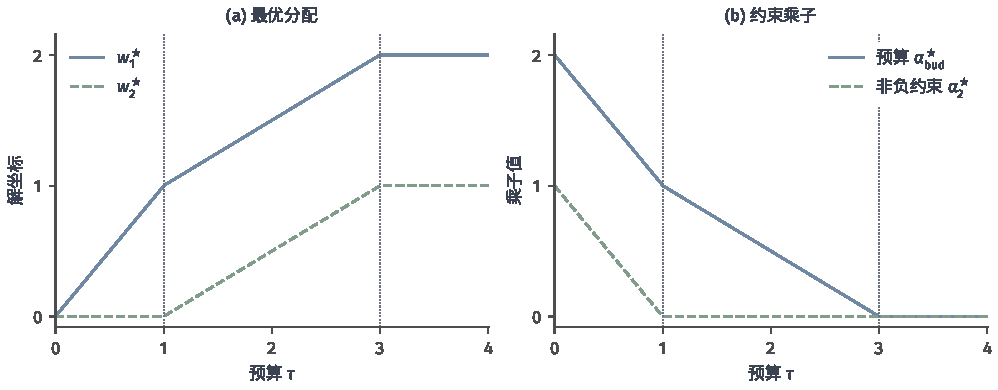
\includegraphics[width=169.0mm]{figures/01-mathematical-preliminaries-upper/01-mathematical-language-combinatorics-analysis-optimization/matplotlib/opt-budget-active-set/figure.pdf}
  \caption{例~\ref{ex:opt-kkt-budget}的解析解。左图为两个最优分配坐标，右图为预算乘子与第二个非负约束的乘子。竖参考线标出$\tau=1,3$；在切换点约束可以取等号而乘子为零，说明活跃性与正价格并不等价。}
 \label{fig:opt-budget-active-set}
\end{figure*}

一般地，设问题依赖参数$\tau$，在一个局部极小点附近固定活跃不等式的指标集$I$。
未活跃乘子恒为零，只把$\bm\alpha_I$作为未知量。将驻点条件、全部等式和活跃不等式的等号条件写成
$\bm\Phi(\bm w,\bm\nu,\bm\alpha_I,\tau)=\bm0$，方程数与未知量数都是$d+m+|I|$。
记这一局部分支为$(\widehat{\bm w},\widehat{\bm\nu},\widehat{\bm\alpha}_I)$。
若$\bm\Phi$连续可微，且对这三组未知量的Jacobian可逆，则第~\ref{chap:mathematical-analysis}章的隐式求导给出
\[
  \frac{d}{d\tau}
  \begin{bmatrix}\widehat{\bm w}\\\widehat{\bm\nu}\\\widehat{\bm\alpha}_I\end{bmatrix}
  =
  -\left(\frac{\partial\bm{\Phi}}
  {\partial(\bm{w},\bm{\nu},\bm{\alpha}_I)}\right)^{-1}
  \frac{\partial\bm{\Phi}}{\partial\tau}.
\]
这个Jacobian是完整KKT系统的导数，原目标Hessian可逆并不足以保证它可逆。活跃集改变或
该矩阵奇异时，解映射可能不可微；此时不能跨越切换点沿用同一个导数。
更具体地，若目标与约束二阶连续可微，记全部等式与活跃不等式的梯度行共同组成$\bm A_I$，并设它满行秩，
则固定活跃集的KKT导数为
\[
 \begin{bmatrix}
 \nabla_{\bm w,\bm w}^2\mathcal L&\bm A_I^\top\\
 \bm A_I&0
 \end{bmatrix}.
\]
若Lagrangian的Hessian在$\ker\bm A_I$上正定，该矩阵可逆：
齐次方程先给$\bm A_I\bm d=0$，与第一行作内积推出$\bm d=0$，
满行秩再迫使乘子增量为零。加上活跃不等式乘子严格为正、未活跃约束有严格余量，
可在小邻域内保持同一活跃集和局部极小分支。
若约束写成$g_k(\bm w)-\tau_k\leq0$而目标不直接依赖$\tau_k$，
定义局部分支值$\widehat V(\bm\tau)=f(\widehat{\bm w}(\bm\tau))$。
对它应用链式法则，并用KKT平衡及活跃约束的导数消去解导数，便得
$\partial\widehat V/\partial\tau_k=-\widehat\alpha_k$，其中未活跃乘子取零。
只有该分支继续为全局最优时，$\widehat V$才等于全局最优值$V$；例如凸问题中满足KKT即可保证这一点。
目标也依赖参数时，还须加入$\partial f/\partial\tau_k$及其余约束的参数项。

惩罚与硬约束有联系，但不是逐参数自动等价。考虑约束问题
\[
  \min_{\bm{w}}f(\bm{w})
  \quad\text{s.t.}\quad
  \lVert\bm{w}\rVert_1\leq R.
\]
若该问题有原始最优解，强对偶成立，并且对偶最优乘子
$\lambda^\star$确实达到，例如满足前述Slater条件且最优值有限，则原始最优解同时最小化
$f(\bm{w})+\lambda^\star\lVert\bm{w}\rVert_1$；Lagrangian中的常数
$-\lambda^\star R$不影响最小点。仅有原、对偶最优值相等并不能保证这样的有限乘子存在。
反过来，不同$\lambda$对应的范数半径可能相同，非凸问题还可能存在对偶间隙。把
$\bm{w}$写成其他参数的函数也会改变优化几何；即使表示同一预测函数，也不保证产生同一
更新轨迹。
反向对应也可以精确说明：若$\widehat{\bm w}$最小化$f+\lambda\|\cdot\|_1$且$\lambda\geq0$，
令$R=\|\widehat{\bm w}\|_1$，则它最小化半径为$R$的约束问题，
因为任何范数不超过$R$且$f$更低的候选都会使惩罚目标更低。
这只构造了与该解匹配的半径，不证明$\lambda$与$R$一一对应。
对一般凸约束，若原始与对偶最优解均达到且对偶间隙为零，取
$\rho>\max\{\|\bm\nu^\star\|_\infty,\|\bm\alpha^\star\|_\infty\}$，
则$f+\rho(\sum_j|a_j|+\sum_k[g_k]_+)$不小于最优Lagrangian，
并对任何非零约束违反多出严格正量。因此有限参数精确惩罚可由达到的乘子支持。
共同二次等式例的$\nu^\star=-16/17$，故$\rho>16/17$的绝对值惩罚已经精确，
与二次惩罚只能在极限可行形成对照。

\section{计算预算有限时的近似优化}
\label{sec:opt-approximate-optimization}

基本更新可以写成一条公式，执行它却需要读取信息、解子问题并重复多轮。若这些成本超过预算，就需要说明简化了什么，以及简化引入的误差如何受控。四种做法回答的是同一个问题——在哪一环上让步：放宽约束改变可行集合；替换每轮目标改变优化对象；拆开变量改变每步的变量范围；近似更新改变梯度或子问题解的信息。让步之后得到的候选仍须按原问题的可行性与误差标准核验，因为每一种简化都只控制被简化后的那个问题。

\subsection{基于约束松弛的近似求解}
\label{sec:opt-relaxations-certificates}

离散选择无法直接套用前面的连续方法，因为可行集合没有凸性，梯度信息也无从谈起。
以第~$\ref{chap:combinatorics}$章的选课为例，变量只能取$0$或$1$，目标在这些孤立点上
谈不上斜率，自然无法沿梯度移动。一种做法是把候选集合换成包含它的连续集合，先求出这个较容易问题的解，再设法回到原问题。
第~\ref{chap:combinatorics}章已利用候选范围的包含关系建立松弛界。
现在还需区分两件事：连续集合能否精确包住原候选，以及返回的连续最优点能否恢复为原问题的解。
把原候选的加权平均一并纳入，可以得到包含这些候选的最小凸集。

\begin{definition}[有限点集的凸包]
\label{def:opt-convex-hull}
设$S=\{\bm s_1,\ldots,\bm s_N\}\subseteq\mathbb R^d$非空。
其凸包（convex hull）由这些点的全部凸组合构成：
\[
  \operatorname{conv}(S)
  =\left\{\sum_{i=1}^N\alpha_i\bm s_i:
  \alpha_i\geq0,\ \sum_{i=1}^N\alpha_i=1\right\}.
\]
\end{definition}
例如离散点集
\[
  S=\{(0,0),(1,0),(0,1)\}
\]
可以表示“至多选择一个项目”。把$S$替换为三角形
\[
  \operatorname{conv}(S)
  =\{(x_1,x_2):x_1,x_2\geq0,\ x_1+x_2\leq1\}
\]
得到\term{凸松弛}（convex relaxation）：原来的每个候选仍可行，但增加了分数候选。
对最小化问题，松弛最优值是原最优值的下界；对最大化问题则是上界。

对于有限非空$S$，精确凸包不改变任意线性目标$\bm{c}^{\top}\bm{x}$的最优值：任意
$\bm{x}=\sum_i\alpha_i\bm{s}_i\in\operatorname{conv}(S)$都满足
$\bm{c}^{\top}\bm{x}=\sum_i\alpha_i\bm{c}^{\top}\bm{s}_i
\geq\min_{\bm{s}\in S}\bm{c}^{\top}\bm{s}$，再结合
$S\subseteq\operatorname{conv}(S)$即得最小值相等，最大值同理。
数值相等仍没有指定求解器返回哪个点：若多个候选都最优，它们的凸组合也最优。

\begin{definition}[凸集的极点]
\label{def:opt-extreme-point}
设$K\subseteq\mathbb R^d$为凸集。若$\bm x\in K$满足：对任何$\bm u,\bm v\in K$
与$\theta\in(0,1)$，只要$\bm x=\theta\bm u+(1-\theta)\bm v$，就有
$\bm u=\bm v=\bm x$，则称$\bm x$为$K$的极点（extreme point）。
\end{definition}
极点不能再由其他可行点的非平凡平均得到。线性目标的所有最优点则组成同一个面。
\begin{definition}[线性目标的最优面]
\label{def:opt-optimal-face}
设线性目标$\bm c^\top\bm x$在非空凸集$K$上达到有限最大值$M$。
其最优面（optimal face）为
\[
  K^\star=\{\bm x\in K:\bm c^\top\bm x=M\}.
\]
最小化时，将$M$换为达到的有限最小值即可。
\end{definition}
当$K=\operatorname{conv}(S)$且$S$有限时，最优面正是$S$中全部最优点的凸包：
若一个凸组合对次优点给了正权重，其线性目标值便严格低于最大值。
若$S\subseteq\mathbb Z^d$，最优面还含有整数极点。可以在有限个整数最优点中，
按坐标次序逐项取最大值，选出一个点。若它是两个可行点的非平凡平均，线性最优性先迫使
这两个点都最优，再逐坐标的最大性迫使它们与所选点相同，因此该点确为极点。

即使如此，返回的最优点仍可能是分数点。例如上面的三角形在目标$x_1+x_2$下，
整条边$x_1+x_2=1$都是最优面，$(1/2,1/2)$也最优；逐坐标向上取整却得到
不属于原点集的$(1,1)$。整数极点的存在不保证任意分数最优点都能直接取整。

精确凸包的完整不等式描述可能难以获得。只保留局部约束通常
得到更大的多面体，计算较容易而界更松。若原问题还含乘积$x_ix_j$，可以引入对称矩阵$\bm X$，
用$X_{i,j}$代替这个乘积。精确表达要求$\bm X=\bm x\bm x^\top$，这是非凸的等式。
将它放宽为
\[
 \begin{bmatrix}1&\bm x^\top\\\bm x&\bm X\end{bmatrix}\succeq0
 \quad\Longleftrightarrow\quad \bm X-\bm x\bm x^\top\succeq0
\]
就得到一种半正定松弛。等价性可由二次型配方核对：该块矩阵在$(t,\bm v)$上的值为
$(t+\bm x^\top\bm v)^2+\bm v^\top(\bm X-\bm x\bm x^\top)\bm v$。
精确乘积总满足新约束，但新约束允许$\bm X$与真实乘积有偏差；原来的其他约束也必须保留或相应转换。
新增矩阵有$O(d^2)$个元素，因而它改善界的可能性伴随着更高的存储和锥约束求解成本。

取整还可能破坏约束。考虑
\[
  \max_{x_1,x_2\in\{0,1\}}x_1+x_2
  \quad\text{s.t.}\quad 2x_1+2x_2\leq3.
\]
整数最优值为$1$，而把变量放宽到$[0,1]$后，$(3/4,3/4)$可行且目标值为$3/2$。
逐坐标四舍五入得到$(1,1)$，却违反容量约束；逐坐标向下取整虽可行，却得到目标值$0$。
因此松弛值、恢复可行性的规则和恢复后的目标损失必须分别分析。

若松弛集合比整数可行点的凸包更大，松弛最优值可能严格优于所有整数可行解；
这种最优值差异称为\term{整数间隙}（integrality gap）。上例采用加法差距时，间隙为
$3/2-1=1/2$。更大的松弛不一定产生严格间隙，它还取决于目标；
精确凸包对线性目标没有这种最优值差异，却仍可能包含分数最优点。

图~\ref{fig:opt-hull-relaxation}固定同一个整数问题，把两种连续可行域并列。
精确凸包上的最优值与整数候选一致；局部容量约束定义的松弛多出了整数候选无法平均
得到的区域。这一多出的区域，才使目标上界从$1$升到$3/2$。
\begin{figure*}[htbp]
  \centering
  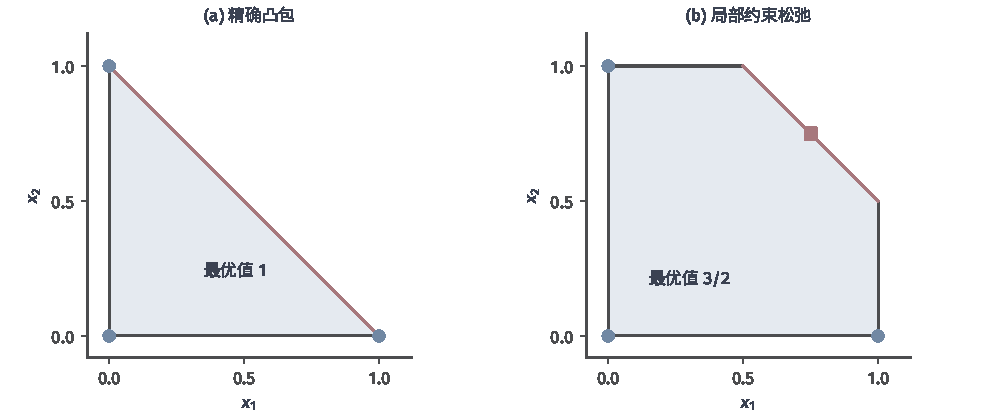
\includegraphics[width=169.0mm]{figures/01-mathematical-preliminaries-upper/01-mathematical-language-combinatorics-analysis-optimization/matplotlib/opt-hull-relaxation/figure.pdf}
  \caption{最大化$x_1+x_2$的两种放宽。左图精确凸包满足$x_1+x_2\leq1$；右图局部松弛满足$0\leq x_i\leq1$与$x_1+x_2\leq3/2$。实心圆为整数可行点，方形为右图的分数最优点$(3/4,3/4)$，粗边标出各自最优面。两图采用相同坐标尺度。}
 \label{fig:opt-hull-relaxation}
\end{figure*}

集合函数的连续扩展也有多种选择。连续变量上的凸性或凹性必须针对所选扩展检验，
不能仅凭原集合函数次模就断言成立；扩展方式决定可用的优化工具。
第~\ref{chap:graph-theory}章会讨论一个可精确求解的特殊情形：二值成对能量满足相应
次模不等式时，可以表示为非负容量的割。一般集合函数的次模性本身，并不保证任意
次模最大化或最小化都能用图割解决。

上面的三角形$\operatorname{conv}(S)$同时说明两件事。原候选$(1,0)\in S$与分数点
$(1/2,1/2)\in\operatorname{conv}(S)\setminus S$在线性目标$x_1+x_2$下都有目标值$1$，
所以这个最优值确实能由原候选取得；但分数点本身不是原问题允许的解。
求解器若返回它，仍需另选或恢复一个属于$S$的最优点。最优数值相同与返回的点原本可行，
是两个不同的保证。

可计算界构成停止证书。对最小化问题，若可行解给出上界$U$，对偶或松弛给出下界$L$，
则
\[
  0\leq U-p^\star\leq U-L.
\]
当$U=L$时已证明全局最优。若把松弛解取整为可行解$\widehat{\bm{x}}$，还应单独分析
$f(\widehat{\bm{x}})-L$；“取整后看起来接近”不是误差界。互补松弛能够证明哪些约束在
最优点活跃的必要关系，却不能仅凭约束活跃就反推正乘子，也不总能直接构造整数解。
图模型中的边缘多面体和MAP松弛会在图与概率对象
建立后复用这里的凸包、上下界和间隙概念。

\subsection{基于代理目标的近似求解}
\label{sec:opt-majorization-improvement}

梯度下降之所以能算出闭式步长，是因为它用一个可计算的二次上界代替了原目标。
这其实是一种“以退为进”：原目标在当前点附近可能形状复杂、没有闭式最优步长，于是先
造一个在当前点与它贴合、但处处盖在它上方的简单函数；把这个简单函数最小化，就能保证
原目标不会变差。若同样的上界来自别的可解结构，这套下降逻辑也能使用，而不要求目标本身是二次函数。
代理函数就是这种用来代替原目标的上界：它必须与目标在当前点取同值、同斜率，并处处不低于目标，
从而保证最小化它不会把原目标推高。
\begin{definition}[主化代理与MM更新]
\label{def:opt-majorization-minimization}
给定目标$F:C\to\mathbb R$、当前点$\bm w^{(t)}\in C$，
\term{主化--最小化方法}（majorization--minimization, MM）在当前点
$\bm{w}^{(t)}$构造代理函数$Q(\bm{w}\mid\bm{w}^{(t)})$，满足
\[
  F(\bm{w})\leq Q(\bm{w}\mid\bm{w}^{(t)}),
  \qquad
  F(\bm{w}^{(t)})=Q(\bm{w}^{(t)}\mid\bm{w}^{(t)}).
\]
上界关系要求对所有$\bm w\in C$成立。若新点$\bm w^{(t+1)}\in C$满足代理值不增，
就称这一步为MM改善更新。
\end{definition}
此时
\begin{align*}
  F(\bm{w}^{(t+1)})
  &\leq Q(\bm{w}^{(t+1)}\mid\bm{w}^{(t)})\\
  &\leq Q(\bm{w}^{(t)}\mid\bm{w}^{(t)})
  =F(\bm{w}^{(t)}).
\end{align*}
第一步用全局上界，第二步用代理改善，最后一步用切触条件。若代理只在当前点附近控制原
目标，而新点走出该邻域，单调链条便会断裂。

下降引理本身给出一个显式代理。若$F$为$L$光滑且$L>0$，可取
\[
  Q(\bm{w}\mid\bm{w}^{(t)})
  =F(\bm{w}^{(t)})
  +\langle\nabla F(\bm{w}^{(t)}),\bm{w}-\bm{w}^{(t)}\rangle
  +\frac{L}{2}\lVert\bm{w}-\bm{w}^{(t)}\rVert_2^2.
\]
它在当前点切触并全局上界$F$。若$C=\mathbb R^d$，精确最小化$Q$恰好得到步长$1/L$的梯度更新；
若$C$是非空闭凸集，配方后得到的是$\Pi_C(\bm w^{(t)}-\nabla F(\bm w^{(t)})/L)$，即投影梯度。仅让代理
与原目标在当前点具有相同梯度，却不满足全局上界，不能推出上面的单调不等式链。

例如$F(x)=x^2/2$、当前点$x^{(t)}=1$，取
$Q(x\mid1)=1/2+(x-1)+(x-1)^2$，则$Q-F=(x-1)^2/2\geq0$且当前点取等号。
代理最小点为$1/2$，于是$F(1/2)=1/8\leq Q(1/2\mid1)=1/4\leq F(1)=1/2$。
图~\ref{fig:opt-majorizer-versus-tangent}把这条链与只有相同局部斜率的切线对照。
\begin{figure}[htbp]
  \centering
  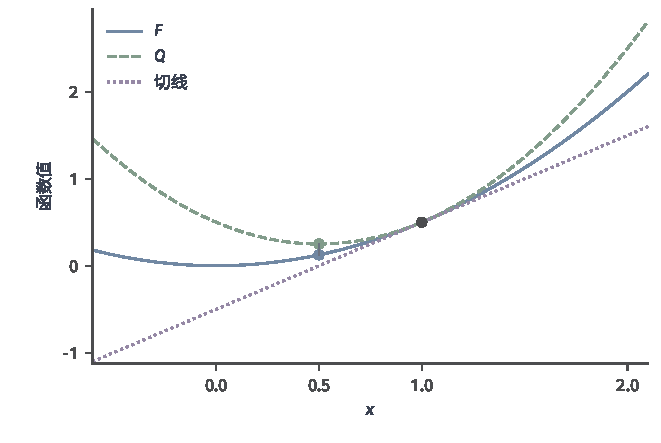
\includegraphics[width=112.0mm]{figures/01-mathematical-preliminaries-upper/01-mathematical-language-combinatorics-analysis-optimization/matplotlib/opt-majorizer-versus-tangent/figure.pdf}
  \caption{代理上界与切线的区别。蓝线为$F(x)=x^2/2$，绿虚线为当前点$1$处的主化代理$Q$，
 紫点线为同点切线$x-1/2$。三者在当前点同值同斜率，但切线位于目标下方，
 最小化它不能使用MM的上界链；绿点标出代理最小点对应的值。图为解析教学示例。}
 \label{fig:opt-majorizer-versus-tangent}
\end{figure}

代理不必精确最小化，但必须分清计算省在何处。记子问题最优值为
\[
 Q^{\star,(t)}=\inf_{\bm w\in C}Q(\bm w\mid\bm w^{(t)}).
\]
若近似子问题解满足
\[
 Q(\bm w^{(t+1)}\mid\bm w^{(t)})\leq Q^{\star,(t)}+\epsilon^{(t)},
\]
则
\[
 \begin{aligned}
 F(\bm w^{(t+1)})&\leq F(\bm w^{(t)})-\Delta^{(t)}+\epsilon^{(t)},\\
 \Delta^{(t)}&=Q(\bm w^{(t)}\mid\bm w^{(t)})-Q^{\star,(t)}\geq0.
 \end{aligned}
\]
只有$\epsilon^{(t)}\leq\Delta^{(t)}$才由此保证本轮原目标不增。实际无需知道$Q^{\star,(t)}$，
也可直接检查新代理值是否低于旧代理值，再决定接受或继续求解。
允许误差超过代理改善时，累计不等式为
$\sum_{t<T}\Delta^{(t)}\leq F(\bm w^{(0)})-\inf_C F+\sum_{t<T}\epsilon^{(t)}$，
其中假设原目标有有限下界。可求和误差控制累计退让，却不自动保证达到全局最优点。

同一数值例中，代理为$Q(x\mid1)=(x-1/2)^2+1/4$。
若只求到$x=3/4$，其代理值为$5/16<1/2$，原目标为$9/32$，仍严格改善；
若返回$x=5/4$，代理误差为$9/16>\Delta^{(t)}=1/4$，原目标反而升为$25/32$。
当任务是最大化$F$时，方向相反：构造切触下界$Q\leq F$，
使$Q(\bm w^{(t+1)}\mid\bm w^{(t)})\geq Q(\bm w^{(t)}\mid\bm w^{(t)})$，
才有$F(\bm w^{(t+1)})\geq Q(\bm w^{(t+1)}\mid\bm w^{(t)})\geq F(\bm w^{(t)})$。
不能沿用最小化的上界方向。

\subsection{基于分块更新的近似求解}
\label{sec:opt-block-alternating-distribution}

若变量自然分成$\bm{u}$与$\bm{v}$两组，可以固定一组更新另一组。设$\bm u\in\mathbb R^p$、$\bm v\in\mathbb R^q$，$\bm X\in\mathbb R^{n\times p}$、$\bm Z\in\mathbb R^{n\times q}$、$\bm y\in\mathbb R^n$，$r$与$s$分别为两组变量的惩罚函数。对
\[
  \Phi(\bm{u},\bm{v})
  =\frac12\lVert\bm{X}\bm{u}+\bm{Z}\bm{v}-\bm{y}\rVert_2^2
  +r(\bm{u})+s(\bm{v}),
\]
\term{分块坐标法}（block coordinate method）每次只对一个块走梯度或近端步；
\term{交替最小化}（alternating minimization）则精确或近似求解每个块的条件子问题。
若每次子问题确实降低同一个
$\Phi$，目标值单调不增。精确交替最小化时，这一点直接来自
\[
  \Phi(\bm{u}^{(t+1)},\bm{v}^{(t)})
  \leq\Phi(\bm{u}^{(t)},\bm{v}^{(t)}),\qquad
  \Phi(\bm{u}^{(t+1)},\bm{v}^{(t+1)})
  \leq\Phi(\bm{u}^{(t+1)},\bm{v}^{(t)}).
\]
但非凸情形下仍可能停在局部解或依赖初始化。

一个可复核的耦合二次例子是
\[
  \Phi(u,v)=\frac12(u-v)^2+\frac12(u-1)^2.
\]
固定$v$时的唯一最优点为$u=(v+1)/2$，固定$u$时的唯一最优点为$v=u$。从
$v^{(0)}$出发，一轮交替更新得到
$u^{(t+1)}=(v^{(t)}+1)/2$、$v^{(t+1)}=u^{(t+1)}$，因而
$v^{(t+1)}-1=(v^{(t)}-1)/2$，最终到达联合最优点$(1,1)$。这里的收敛来自这个
正定二次目标的特殊结构。换成非凸目标$(uv-1)^2$并从$(0,0)$开始时，逐块目标在一块
固定为零时没有提供离开零点的理由；若平局规则继续选择零，目标保持为$1$，而全局最优值
为$0$。所以逐块精确和目标单调都不单独保证全局最优。
若无约束目标连续可微，一个点对每一块都已精确最优，则各块偏导同时为零，故它是驻点。
目标联合凸时，这又足以推出全局最优；仅对各块分别凸则不够。
上述$(uv-1)^2$在另一块固定时都是凸二次函数，仍给出了失败例。
对于实际迭代，还须证明它确实收敛到块最优点，而非仅看到目标值收敛。

约束耦合时，可以复制共享变量，再通过一致性约束分解为局部子问题。乘子负责协调副本，
这改变了每步计算位置，却没有删除原约束。若局部问题没有被足够准确地求解，或协调步长
不满足条件，分解形式本身不保证收敛。
具体地，最小化$r(\bm w)+s(\bm w)$可改写为
$\min_{\bm u=\bm v}\{r(\bm u)+s(\bm v)\}$。固定等式乘子$\bm\nu$后，
两项Lagrangian子问题可独立求解：
\begin{align}
 \bm u^{(t)}&\in\argmin_{\bm u}\{r(\bm u)+\langle\bm\nu^{(t)},\bm u\rangle\},\nonumber\\
 \bm v^{(t)}&\in\argmin_{\bm v}\{s(\bm v)-\langle\bm\nu^{(t)},\bm v\rangle\},\nonumber\\
 \bm\nu^{(t+1)}&=\bm\nu^{(t)}+\eta^{(t)}(\bm u^{(t)}-\bm v^{(t)}).
 \label{eq:opt-consensus-dual-decomposition}
\end{align}
输入是两个可分函数及当前价格，子问题输出各自副本，协调量是副本差。
与前一节的交替最小化不同，局部副本可以暂时不一致，所改进的是对偶下界，
因此原始目标并不保证每轮下降；这是使用分解时最容易误解的一点。若两个子问题适当闭凸且强凸，解总存在，
负对偶函数的光滑常数可取$1/\mu_r+1/\mu_s$，步长据此选择；
仅凸时则回用有界残差的对偶次梯度分析。子问题无下界时，这种分解不能直接执行。

取$r(u)=(u-1)^2/2$、$s(v)=(v+1)^2/2$，
内层解是$u=1-\nu$、$v=\nu-1$，对偶函数$q(\nu)=2\nu-\nu^2$。
令$\nu^{(0)}=0$、$\eta^{(t)}=1/4$，得到
$\nu^{(t)}=1-2^{-t}$、$u^{(t)}=2^{-t}$、$v^{(t)}=-2^{-t}$。
第一轮两个副本各自使局部目标为零，却相差$2$；第三次取值为$1/4,-1/4$，
差缩小到$1/2$。将二者平均为共同变量$w=0$，恢复可行上界$r(0)+s(0)=1$，
与$q(\nu^{(t)})=1-4^{-t}$之间的差为$4^{-t}$。
这里的平均恰好最优来自对称二次结构，不是一般副本问题的免费恢复规则。

若每轮只保证
$\mathcal L(\widetilde{\bm w}^{(t)},\bm y^{(t)})\leq q(\bm y^{(t)})+\epsilon^{(t)}$，
将该候选代入另一组乘子会给
\[
 q(\bm y')\leq q(\bm y^{(t)})
 +\langle\widetilde{\bm s}^{(t)},\bm y'-\bm y^{(t)}\rangle+\epsilon^{(t)}.
\]
于是投影次梯度的单步距离界多出$2\eta^{(t)}\epsilon^{(t)}$。累加后，
有限步界的分子应增加
\[
 2\sum_{t<T}\eta^{(t)}\epsilon^{(t)}.
\]
近似内层值本身大于等于$q$，不能直接冒充原问题下界。有可信子问题误差界时，
可用下界为
\[
 \mathcal L(\widetilde{\bm w}^{(t)},\bm y^{(t)})-\epsilon^{(t)}.
\]

变量也可以是一个分布$q$。此时“更新分布”仍是在某个可行分布集合上降低同一目标，而非
一种脱离优化的概率操作。在有限支持$\{1,\ldots,m\}$上，分布变量就是概率单纯形
\[
  \bm{\Delta}_m
  =\{\bm{q}\in\mathbb{R}^m:q_i\geq0,\ \sum_{i=1}^m q_i=1\}.
\]
归一化、非负性和支持集都是可行约束，更新后必须仍留在这个单纯形中。
例如块子问题$\min_{\bm q\in\bm\Delta_2}\|\bm q-(0.8,0.4)^\top\|_2^2/2$
的解不是原向量：为使两坐标和为$1$，各减去$0.1$，得到$(0.7,0.3)^\top$；
非负性仍成立，因此它满足该凸投影问题的最优性条件。
EM与变分方法还需要
期望、条件分布和散度，相关对象可参考\BookChapterRef{chap:random-variables}{卷2《数学准备：概率、因果与决策》第1章“随机变量”}和
\BookChapterRef{chap:information-theory-and-statistical-geometry}{卷2《数学准备：概率、因果与决策》第2章“概率分布”}。
这些方法将复用交替优化与MM的单调性核对方式。

\subsection{基于近似更新的求解}
\label{sec:opt-stochastic-gradient-stability}

有限和目标
\[
  F_S(\bm{w})=\frac1n\sum_{i=1}^n\ell_i(\bm{w})
  +\frac{\lambda}{2}\lVert\bm{w}\rVert_2^2
\]
的经验损失梯度要读取全部$n$项。这里的抽取先只用有限概率权重理解，$\mathbb E_I$表示按这些权重求和。
随机迭代的收敛还需要步长、累计噪声与平均动力学条件，可参考
\BookChapterRef{chap:action-and-state}{卷2《数学准备：概率、因果与决策》第4章“动力系统”}。
若$I$在$\{1,\ldots,n\}$上均匀抽取，则完整目标的
随机梯度可取
\[
  \bm{g}_I(\bm{w})
  =\nabla\ell_I(\bm{w})+\lambda\bm{w},\qquad
  \mathbb{E}_I[\bm{g}_I(\bm{w})]
  =\nabla F_S(\bm{w}).
\]
若按概率$p_i>0$非均匀抽取，则应改用
\[
  \bm{g}_I(\bm{w})
  =\frac{\nabla\ell_I(\bm{w})}{np_I}+\lambda\bm{w}.
\]
正则项梯度$\lambda\bm{w}$是确定量，无需抽样；小批量只需平均若干经过相应加权的
损失梯度，再加上这项确定梯度。
例如$n=2$、当前位置两项标量梯度为$2,-1$，完整损失梯度为$1/2$。
若以$p_1=3/4,p_2=1/4$抽样而不重加权，均值为$5/4$，已经改变更新方向的大小；
使用$1/(np_I)$后，两种输出为$4/3,-2$，均值恢复为$1/2$。

在第$t$轮固定已经得到的历史和当前点，再按该轮概率求有限加权平均，记作$\mathbb E^{(t)}$。
无偏性要求的是这个固定历史后的平均，不只是对一个与迭代无关的固定点成立。
若固定历史后的各抽样梯度独立同分布、无偏，且均方波动不超过$(\sigma^{(t)})^2$，
将$b$个样本平均后，交叉误差项均值为零，故
\[
 \mathbb E^{(t)}\left\|\frac1b\sum_{j=1}^b\bm g_{I_j}
             -\nabla F_S(\bm w^{(t)})\right\|_2^2
 \leq\frac{(\sigma^{(t)})^2}{b}.
\]
这解释了小批量减少波动但增加信息读取量的取舍；重复使用同一个样本$b$次没有这一收益。
有偏近似可写成$\bm g^{(t)}=\nabla F_S(\bm w^{(t)})+\bm b^{(t)}+\bm\xi^{(t)}$，
其中$\bm b^{(t)}=\mathbb E^{(t)}\bm g^{(t)}-\nabla F_S(\bm w^{(t)})$、
$\mathbb E^{(t)}\bm\xi^{(t)}=0$。
抽样降低的是波动，不会自动消除$\bm b^{(t)}$。这里仅建立逐轮有限加权接口，
长期随机收敛仍需后文的条件期望工具。

在概率工具建立前，可以先分析带确定误差的更新
\[
  \bm{w}^{(t+1)}
  =\bm{w}^{(t)}-\eta^{(t)}
  \bigl(\nabla F(\bm{w}^{(t)})+\bm{e}^{(t)}\bigr).
\]
若$F$为$L$光滑，其中$L>0$，且$0<\eta^{(t)}\leq1/L$，令$\bm g=\nabla F(\bm w^{(t)})$，
下降引理给出的变化上界为
$-\eta^{(t)}\|\bm g\|_2^2-\eta^{(t)}\langle\bm g,\bm e^{(t)}\rangle
+L(\eta^{(t)})^2\|\bm g+\bm e^{(t)}\|_2^2/2$。
将$L(\eta^{(t)})^2$放宽为$\eta^{(t)}$后，平方展开的交叉项恰好抵消，得到
\[
  F(\bm{w}^{(t+1)})
  \leq F(\bm{w}^{(t)})
  -\frac{\eta^{(t)}}{2}\lVert\nabla F(\bm{w}^{(t)})\rVert_2^2
  +\frac{\eta^{(t)}}{2}\lVert\bm{e}^{(t)}\rVert_2^2.
\]
误差项因而必须与所求结论一起累计。固定非零偏差通常只允许迭代接近一个误差邻域；
$\sum_t\eta^{(t)}\lVert\bm{e}^{(t)}\rVert_2^2<\infty$使上述目标下降不等式中的累计
误差项有限。仅令
$\eta^{(t)}\to0$仍不够，还要核对步长总量是否足以持续纠偏，以及目标与迭代是否保持稳定。
若$F_{\inf}>-\infty$，求和得到一个可直接使用的有限预算界：
\begin{equation}
 \min_{t<T}\|\nabla F(\bm w^{(t)})\|_2^2
 \leq\frac{2(F(\bm w^{(0)})-F_{\inf})
             +\sum_{t<T}\eta^{(t)}\|\bm e^{(t)}\|_2^2}
            {\sum_{t<T}\eta^{(t)}}.
 \label{eq:opt-inexact-gradient-finite-rate}
\end{equation}
步长总和发散且加权平方误差和有限时，右侧趋零；结论仍只涉及最佳驻点残差。
例如$F(w)=w^2/2$、恒定误差$e\neq0$与$0<\eta<2$给
$w^{(t+1)}=(1-\eta)w^{(t)}-\eta e$，最终趋向$-e$而非$0$。
固定偏差即使很小，也会留下$e^2/2$的目标差。

若理想更新映射$T^{(t)}(\bm{w})=\bm{w}-\eta^{(t)}\nabla F(\bm{w})$是
$\rho^{(t)}$-Lipschitz，实际轨迹与理想轨迹之差$\delta^{(t)}$满足
\begin{equation}
  \delta^{(t+1)}\leq\rho^{(t)}\delta^{(t)}+\eta^{(t)}\lVert\bm{e}^{(t)}\rVert_2.
  \label{eq:opt-inexact-gradient-recurrence}
\end{equation}
令$a^{(t)}=\eta^{(t)}\|\bm e^{(t)}\|_2$，完整展开为
\[
 \delta^{(T)}\leq\left(\prod_{j=0}^{T-1}\rho^{(j)}\right)\delta^{(0)}
 +\sum_{t=0}^{T-1}a^{(t)}\prod_{j=t+1}^{T-1}\rho^{(j)},
\]
其中空积为$1$。若存在统一$\bar\rho<1$使$\rho^{(t)}\leq\bar\rho$，
旧误差几何衰减；$a^{(t)}\to0$还保证$\delta^{(T)}\to0$，
而$a^{(t)}\leq a$只能给出极限上界$a/(1-\bar\rho)$。
证明前一结论时，可把误差和分成有限的早期项与足够小的尾项：早期项的传播因子趋零，
尾项由几何级数控制。仅有每个$\rho^{(t)}<1$不够，例如
$\rho^{(t)}=1-1/(t+2)^2$的前$T$项乘积为$(T+2)/(2(T+1))$，趋向$1/2$而非零。

若只有$\rho^{(t)}\leq1$，则$\delta^{(T)}\leq\delta^{(0)}+\sum_{t<T}a^{(t)}$。
控制这条轨迹偏差需要一次范数误差和，而平方误差可求和不蕴含它：取$\eta^{(t)}=1$、
$\|\bm e^{(t)}\|_2=1/(t+1)$即可区分。即使一次范数和有限，也只保证偏差有界，
不保证两条轨迹最终重合。
若$\rho^{(t)}>1$，传播因子还可能放大早期扰动；减小步长同时影响误差注入和理想收敛，需一起计算。

映射系数也必须由目标条件取得。一般$L$光滑目标只能直接给出$\rho^{(t)}\leq1+\eta^{(t)}L$。
若$F$还凸，则梯度满足
\[
 \langle\nabla F(\bm x)-\nabla F(\bm y),\bm x-\bm y\rangle
 \geq\frac1L\|\nabla F(\bm x)-\nabla F(\bm y)\|_2^2.
\]
为证明它，对凸光滑函数$h_{\bm y}(\bm z)=F(\bm z)-\langle\nabla F(\bm y),\bm z\rangle$
使用下降引理；$\bm y$为其全局最小点，故
$h_{\bm y}(\bm x)-h_{\bm y}(\bm y)\geq
\|\nabla F(\bm x)-\nabla F(\bm y)\|_2^2/(2L)$。
交换$\bm x,\bm y$后相加即得所需不等式。再展开两次梯度更新的距离平方，得到
\[
 \|T^{(t)}(\bm x)-T^{(t)}(\bm y)\|_2^2
 \leq\|\bm x-\bm y\|_2^2
 -\eta^{(t)}(2/L-\eta^{(t)})\|\nabla F(\bm x)-\nabla F(\bm y)\|_2^2.
\]
因此$0\leq\eta^{(t)}\leq2/L$时非扩张。若进一步二阶连续可微且
$\mu\bm I\preceq\nabla^2F\preceq L\bm I$，沿两点线段平均Hessian可得
$\rho^{(t)}\leq\max\{|1-\eta^{(t)}\mu|,|1-\eta^{(t)}L|\}$。
固定$0<\eta<2/L$才给出统一小于$1$的系数；变步长需检查其乘积而不是只逐项检查。

同一递推也能比较两组只相差一个训练样本的训练输出。记两组训练样本为$S,S'$，让两条迭代采用相同初值和相同抽样索引：读到共同样本时，更新差异只来自当前位置；读到替换项时，再加入两项样本梯度的差。这样才能把样本替换写成轨迹扰动。具体地，设每个样本梯度
$L$-Lipschitz且在所访问点范数不超过$G$，暂取$\lambda=0$，
两条迭代使用相同索引$I^{(t)}$。记距离为$\Delta^{(t)}$；
若$I^{(t)}$不是被替换的索引，则
\[
  \Delta^{(t+1)}\leq(1+\eta^{(t)}L)\Delta^{(t)};
\]
若恰好抽到被替换项，则再增加至多$2\eta^{(t)}G$。若进一步假设两组数据的每个样本损失都凸，且$0\leq\eta^{(t)}\leq2/L$，
每个样本的梯度更新由刚才的证明为非扩张映射，从而去掉前式中的膨胀因子。经验目标凸本身不足以替代逐样本凸性。
在均匀抽样且固定历史后，被替换索引出现的权重为$1/n$，故
$\mathbb E^{(t)}\Delta^{(t+1)}\leq\Delta^{(t)}+2\eta^{(t)}G/n$。
相同初值给$\mathbb E\Delta^{(T)}\leq(2G/n)\sum_{t<T}\eta^{(t)}$。
若测试损失在比较点之间为$K$-Lipschitz，损失差再被$K\Delta^{(T)}$控制；
参数接近与预测或损失接近仍需这一接口。这给出\term{算法稳定性}（algorithmic stability）的一种具体界：
对固定的相邻数据集$S,S'$，在两条轨迹使用相同随机索引的耦合下，算法随机性所产生的
期望参数距离不超过$(2G/n)\sum_{t<T}\eta^{(t)}$；固定测试样本上的期望损失差绝对值
不超过这个量乘以$K$。这里没有对数据集或测试样本再取平均。
若要使上界对所有相邻数据集和所有测试样本统一成立，还须使$L,G,K$及步长条件在这些对象上统一成立。
上述期望递推的严格表述需要条件期望，以固定已经得到的历史再取平均；
随机迭代本身的收敛还需步长、累计噪声与平均动力学条件，不能由算法稳定性直接推出。

缩放损失会等比例缩放梯度，因此学习率不能脱离损失尺度比较。梯度裁剪把过大更新限制在
指定半径内，改变了估计量并可能引入偏差。
具体地，阈值$c>0$下令
$\operatorname{clip}_c(\bm g)=\bm g\min\{1,c/\|\bm g\|_2\}$，并令零向量仍映为零。
前述等概率标量梯度$2,-1$的均值为$1/2$，裁剪到$c=1$后变成$1,-1$，
均值为零；这展示了偏差怎样产生。第~\ref{sec:opt-penalty-methods}节比较过的权重衰减也会改变更新：
若本来要对$f+\lambda\|\bm w\|_2^2/2$作预条件更新，却使用直接衰减，
实际每步减去的向量为$\eta(\bm P\nabla f+\lambda\bm w)$，
相对预期向量$\eta\bm P(\nabla f+\lambda\bm w)$多出$\eta\lambda(\bm I-\bm P)\bm w$。这是一项确定差异，增加抽样批量无法消除。

前面的稳定性界需要沿途梯度范数上界$G$。当样本损失非负且光滑时，可以改从沿途损失值取得这项控制：
若$\ell(\bm w)\leq B$，下面的引理给出$\|\nabla\ell(\bm w)\|_2\leq\sqrt{2LB}$。
它只在损失值已有上界的点上提供梯度界，不声称所有光滑损失的梯度都全局有界。

\begin{lemma}[非负光滑函数的梯度自界]
\label{lem:opt-self-bounding}
若$\ell:\mathbb{R}^d\to[0,\infty)$可微且$L$光滑，其中$L>0$，则
\[
  \lVert\nabla\ell(\bm{w})\rVert_2^2\leq2L\ell(\bm{w}).
\]
\end{lemma}

\begin{proof}
在下降引理中取
$\bm{v}=\bm{w}-\nabla\ell(\bm{w})/L$，得到
\[
  \ell(\bm{v})
  \leq\ell(\bm{w})-\frac{1}{2L}
  \lVert\nabla\ell(\bm{w})\rVert_2^2.
\]
左侧非负，移项即得结论。若损失可取负值，这一步失效；给函数加常数虽不改变梯度，却会
改变右侧，所以非负性是实质条件。
\end{proof}

给定总预算，松弛应返回可行恢复与上下界，代理应核验原目标而非只报子问题收敛，
分块应核验联合驻点或副本一致性，近似更新应核验误差累计。
这些检查可以共用前面的下降和距离递推，但不能互换输出含义：
距离某条理想轨迹很近，不代表那条轨迹本身全局最优；对偶值很高，也不代表本轮原始候选可行。
比较总成本时，应同时计入试探次数、样本读取、局部子问题和恢复步骤，而非只比较外层迭代轮数。

\section{多目标、对抗与双层优化}
\label{sec:opt-decomposition-multiple-levels}

前面固定了比较候选的标量目标，只改变求解方法。若任务同时评价多个指标，就没有现成的
标量来排出全局的高低；若包含两方相反的选择，一方收益即对方代价；若必须先求解一个
问题再评价另一个问题，外层甚至看不到完整的目标函数。这三种情形的共同点是：
“最优答案”的含义本身需要重新规定。多目标问题需要规定如何取舍，极小极大问题需要
规定选择次序，双层问题需要规定内层如何选解。下面建立这些问题各自的比较关系，再讨论可用计算。

\subsection{多目标优化}
\label{sec:opt-multiobjective-saddle}

前面固定了比较候选的标量目标，因此“最优”有明确含义。若同时关心预测精度和计算时间，
两者往往互相牵制，不存在一个数能同时概括两项指标；此时“最优”本身还没有定义，
必须先规定怎样在两个指标之间取舍。如果方案$A$在两项指标上都不差于方案$B$，且至少一项严格优于$B$，
我们就说$A$支配$B$，可以放心淘汰$B$；但如果$A$精度更高而$B$时间更短，两者互不
支配，淘汰谁都会丢掉一项优势。无法被淘汰的方案组成Pareto最优集合。下面把这个
直觉写成定义。
\begin{definition}[支配与Pareto最优]
\label{def:opt-pareto-optimality}
设$C$为非空可行集合，损失向量为
\[
 \bm f=(f_1,\ldots,f_m):C\to\mathbb R^m,
\]
各分量均要最小化。
若$\bm u,\bm v\in C$满足所有$i$都有$f_i(\bm u)\leq f_i(\bm v)$，且至少一项严格小于，
就称$\bm u$\term{支配}（dominate）$\bm v$。不可被任何可行方案支配的点称为
\term{Pareto最优}（Pareto optimal）。
\end{definition}
分量逐项不大于在损失向量上给出偏序；不同参数若产生相同损失向量，仍无法按损失区分。
这里的支配是相应的严格比较，不是单一排名。
下文先用两个目标说明这种区别。

加权和$\alpha f_1+(1-\alpha)f_2$把偏好写成一个标量目标，$\alpha\in[0,1]$。
给定权重后，就可按该标量目标的光滑性、凸性及约束选择前面的求解方法。
若所有权重严格为正，任何全局最小点都为Pareto最优：
支配它的候选会使加权目标严格下降，造成矛盾。
允许零权重时，只能保证不存在所有分量都严格下降的候选，通常称为弱Pareto最优。
把所有可行方案的损失向量放在一起，得到目标像$\bm f(C)=\{(f_1(\bm w),f_2(\bm w)):\bm w\in C\}$；
其中不被其他向量支配的部分称为Pareto前沿。固定权重后，等值线
$\alpha u+(1-\alpha)v=c$以权重向量为法向量，最小化加权损失就是寻找与目标像相交的最低等值线。
这条线只接触目标像在该方向上的支撑点，可能漏掉非凸前沿中的其他Pareto点。
例如三个可行方案的损失向量分别为$(0,1)$、$(1,0)$和$(0.6,0.6)$。第三个方案不被
前两个方案支配，所以是Pareto最优；但对任意$\alpha\in[0,1]$，前两个方案的加权损失
中至少一个不超过$0.5$，严格小于第三个方案的$0.6$，故权重和永远不会选择第三个方案。图~\ref{fig:opt-pareto-weighted-sum}标出这三个方案及一条等值线。

\begin{figure}[htbp]
  \centering
  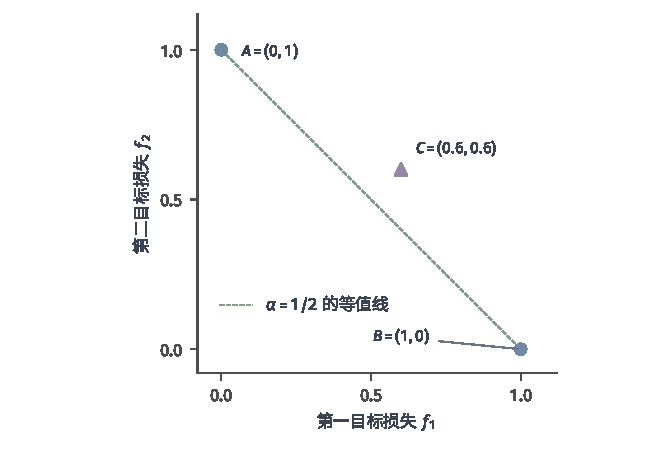
\includegraphics[width=112.0mm]{figures/01-mathematical-preliminaries-upper/01-mathematical-language-combinatorics-analysis-optimization/matplotlib/opt-pareto-weighted-sum/figure.pdf}
  \caption{三个精确可行损失向量，两个目标均需最小化。$A,B,C$互不支配，但对任意$\alpha\in[0,1]$，$C$的加权损失$0.6$都严格大于$\min\{\alpha,1-\alpha\}$。绿虚线仅为$\alpha=1/2$时通过$A,B$的等值线，线上其余点不属于这里的可行集合。因此，Pareto最优不保证能由加权和选到。}
  \label{fig:opt-pareto-weighted-sum}
\end{figure}


在当前点，方向$\bm{d}$若满足
\[
  \langle\nabla f_1(\bm{w}),\bm{d}\rangle<0,\qquad
  \langle\nabla f_2(\bm{w}),\bm{d}\rangle<0,
\]
就是\term{共同下降方向}（common descent direction）。寻找最小范数凸组合
$\alpha\nabla f_1+(1-\alpha)\nabla f_2$相当于把原点投影到两梯度的线段上。

\begin{theorem}[无共同下降方向的一阶判定]
\label{thm:opt-common-descent}
对可微的$m$个目标，在无约束点$\bm{w}$处不存在共同严格下降方向，当且仅当存在
$\alpha_i\geq0$、$\sum_i\alpha_i=1$，使
$\sum_i\alpha_i\nabla f_i(\bm{w})=\bm{0}$。
\end{theorem}

\begin{proof}
若这样的凸组合存在，而$\bm{d}$使每个内积都为负，则加权和内积也为负，与零向量矛盾。
反之，若原点不在梯度集合的凸包中，定理~\ref{thm:opt-projection-separation}给出
$\bm{d}$，使它与每个梯度的内积具有同一严格符号；必要时取$-\bm{d}$，便得到共同严格
下降方向。
\end{proof}

这个条件只排除局部的一阶共同改善，不保证全局Pareto最优；高阶变化或远处方案仍可能
同时改善所有目标。
例如两个目标都为$-x^2$，在$0$的梯度均为零，任意小的非零移动却使两者同时改善。
若目标都凸，零梯度凸组合使相应加权和全局最优，
从而保证弱Pareto最优；要据此得到前面定义的Pareto最优，严格正权重是一条充分条件。
零权重不能省略检查，例如$f_1(x)=0$、$f_2(x)=x^2$在$x=1$满足该一阶判据，
但被$x=0$支配。

共同下降不只是判据，还能给出具体更新。计算权重子问题
\[
 \bm\alpha^\star\in\argmin_{\bm\alpha\in\bm\Delta_m}
 \frac12\left\|\sum_{i=1}^m\alpha_i\nabla f_i(\bm w)\right\|_2^2,
 \qquad
 \bar{\bm g}=\sum_i\alpha_i^\star\nabla f_i(\bm w).
\]
有限梯度的凸包紧且凸，故$\bar{\bm g}$就是原点的唯一投影。
投影最优性给
$\langle\bar{\bm g},\nabla f_i(\bm w)-\bar{\bm g}\rangle\geq0$。
若$\bar{\bm g}\neq0$，取$\bm d=-\bar{\bm g}$便有
$\langle\nabla f_i,\bm d\rangle\leq-\|\bar{\bm g}\|_2^2$对全部$i$成立。
每个目标均$L_i$光滑且$L_i>0$时，任意$0<\eta<2/\max_i L_i$都使
$\bm w^+=\bm w+\eta\bm d$同时降低全部目标；未知常数时，可回溯直至所有目标的
充分下降检验同时通过。若$\bar{\bm g}=0$，算法返回的只是上述一阶证书。
有约束时还要限制$\bm d$的可行性，不能直接使用无约束梯度凸包判据。

例如$f_1(x,y)=((x-1)^2+y^2)/2$、$f_2(x,y)=((x+1)^2+y^2)/2$。
在$(0,1)$两梯度为$(-1,1),(1,1)$，最小范数平均为$(0,1)$；
步长$1$将点移到$(0,0)$，两项目标都由$1$降为$1/2$。
此时梯度为$(-1,0),(1,0)$，原点已在它们之间，不能再共同下降。
加权标量问题的解为$(2\alpha-1,0)$，展示了改变权重怎样沿同一条取舍曲线选择答案。

\subsection{极小极大优化}
\label{sec:opt-minimax}

多目标问题在同一组变量上比较若干指标；若这些指标分属对立的两方，一方收益就是另一方的
损失，比较关系就从“无法同时改善”变成“同时选择”。
这种结构在机器学习里很常见：生成对抗网络中生成方想造假、判别方想识破；鲁棒训练中我们想
降低损失，而数据中的扰动方想抬高损失。写成统一形式时，决策者必须先选定自己的策略，
对手看到这个策略后再选最狠的回应，因此决策要按“最坏情况下我仍有多好”来评价。这类问题让两个变量方向相反：
\[
  \min_{\bm{w}\in W}\max_{\bm{z}\in Z}\phi(\bm{w},\bm{z}).
\]
外层先选择$\bm w$，内层在看到它后选择使损失最大的$\bm z$。
因此外层实际最小化最坏响应值，不是让两方分别寻找$\phi$的普通最小点。
倒转次序一般会改变值，原始问题返回的是应对最坏响应的决策；
若还返回一对互为最优响应的候选，则需核验下面的鞍点关系。
\begin{definition}[极小极大鞍点]
\label{def:opt-minimax-saddle}
设$W,Z$非空，$\phi:W\times Z\to\mathbb R$。点$(\bm w^\star,\bm z^\star)\in W\times Z$若对所有
$\bm w\in W,\bm z\in Z$满足
\[
  \phi(\bm{w}^{\star},\bm{z})
  \leq\phi(\bm{w}^{\star},\bm{z}^{\star})
  \leq\phi(\bm{w},\bm{z}^{\star})
\]
就称为\term{极小极大鞍点}（minimax saddle point）。
\end{definition}
这里“鞍点”描述两个变量承担
相反优化方向时的全局比较关系，不是第~\ref{sec:analysis-second-order-curvature}节中
由单个标量函数的驻点和Hessian矩阵正负曲率定义的微分鞍点。微分鞍点未必求解某个极小
极大问题；极小极大鞍点位于边界或目标不可微时，也未必满足驻点与Hessian判据。
对任意候选对定义
\[
  P(\bm{w})=\sup_{\bm{z}\in Z}\phi(\bm{w},\bm{z}),\qquad
  D(\bm{z})=\inf_{\bm{w}\in W}\phi(\bm{w},\bm{z}).
\]
总有$D(\bm{z})\leq P(\bm{w})$，所以
$P(\bm{w})-D(\bm{z})\geq0$是\term{原始--对偶间隙}
（primal--dual gap）；间隙为零时，该候选对满足鞍点不等式。

本章采用以下有限维极小极大版本：若$W,Z$非空、紧且凸，$\phi$连续，对固定
$\bm{z}$的$\phi(\cdot,\bm{z})$为凸函数，对固定$\bm{w}$的
$\phi(\bm{w},\cdot)$为凹函数，则
\[
  \min_{\bm{w}\in W}\max_{\bm{z}\in Z}\phi(\bm{w},\bm{z})
  =
  \max_{\bm{z}\in Z}\min_{\bm{w}\in W}\phi(\bm{w},\bm{z}),
\]
且两侧最值达到。紧致性提供最值的达到，凸凹性允许用分离比较混合候选，连续性保证极限
不丢失函数值。

可以用前面的分离工具说明交换为何成立。记左侧值为$v$，任取$c<v$。
每个$\bm w\in W$都存在$\bm z$使$\phi(\bm w,\bm z)>c$；
连续性与$W$的紧性给出有限个$\bm z_1,\ldots,\bm z_k$，使每个$\bm w$至少在其中一项超过$c$。
考虑向上封闭的集合
\[
 U=\{\bm a\in\mathbb R^k:\text{存在 }\bm w\in W,\
          \phi(\bm w,\bm z_i)\leq a_i\text{ 对全部 }i\}.
\]
各目标关于$\bm w$凸使$U$凸；$\bm a$的收敛序列所对应的$\bm w$可取收敛子列，
故$U$闭。点$c\bm1$不属于$U$，严格分离给出
$\langle\bm\alpha,c\bm1\rangle<
\inf_{\bm a\in U}\langle\bm\alpha,\bm a\rangle$。
向上封闭迫使$\bm\alpha\geq0$，可归一化为$\sum_i\alpha_i=1$。
于是$\inf_{\bm w}\sum_i\alpha_i\phi(\bm w,\bm z_i)>c$。
令$\bar{\bm z}=\sum_i\alpha_i\bm z_i\in Z$，关于$\bm z$的凹性给
$\phi(\bm w,\bar{\bm z})\geq\sum_i\alpha_i\phi(\bm w,\bm z_i)$，
所以右侧极大极小值大于$c$。令$c\uparrow v$再结合弱对偶，即得值相等。
连续函数在紧积空间上一致连续，使$P,D$分别连续并达到最值；
各取一个达到点就由$D\leq\phi\leq P$得到鞍点。

原始与对偶最优解也可形成这一关系：若零对偶间隙、原始与对偶最优解均达到，
则$\mathcal L(\bm w^\star,\bm y)\leq
\mathcal L(\bm w^\star,\bm y^\star)\leq\mathcal L(\bm w,\bm y^\star)$。
这是Lagrangian的全局鞍点，不是原目标$f$自身的微分鞍点。
鲁棒优化中的$\bm{z}$表示最坏扰动，对抗训练让扰动方提高损失，多任务协调
则可能在权重与模型间形成极小极大结构。若缺少上述条件，两个优化次序可能不同；即使值相等，
具体梯度下降--上升仍可能旋转或发散，值的存在定理不等于算法收敛定理。

取$W=Z=[-1,1]$和$\phi(x,z)=xz$，就能复算这种差别。
$P(x)=|x|$、$D(z)=-|z|$，唯一鞍点为$(0,0)$，候选间隙为$|x|+|z|$。
若两方都作普通最小化，会偏好乘积为$-1$的角点，但在该处最大化方立刻有动机反向行动。
若取同时下降与上升
\[
 x^{(t+1)}=x^{(t)}-\eta z^{(t)},\qquad
 z^{(t+1)}=z^{(t)}+\eta x^{(t)},
\]
暂不投影时有
$(x^{(t+1)})^2+(z^{(t+1)})^2=(1+\eta^2)((x^{(t)})^2+(z^{(t)})^2)$。
每个非零初值都向外旋转。加上盒投影也不保证收敛：
$\eta=1$、初值$(1,0)$时依次得到
$(1,1),(0,1),(-1,1),(-1,0),(-1,-1),(0,-1),(1,-1),(1,0)$，
此后重复，鞍点间隙始终不小于$1$。

一种修正是先试探双方响应，再用试探点的方向更新原点，称为外梯度（extragradient）更新。
记$\bm u=(x,z)^\top$、$\bm F(\bm u)=(z,-x)^\top$、$K=W\times Z$，每轮计算
\[
 \bar{\bm u}^{(t)}=\Pi_K(\bm u^{(t)}-\eta\bm F(\bm u^{(t)})),\qquad
 \bm u^{(t+1)}=\Pi_K(\bm u^{(t)}-\eta\bm F(\bar{\bm u}^{(t)})).
\]
这需要两次方向求值与两次投影。对当前双线性例，在投影未激活时，
更新矩阵为
$\left[\begin{smallmatrix}1-\eta^2&-\eta\\ \eta&1-\eta^2\end{smallmatrix}\right]$，
距离平方每步乘以$1-\eta^2+\eta^4<1$（$0<\eta<1$）。
例如$\eta=1/2$且$\|\bm u^{(0)}\|_2\leq1/2$时，
试探点范数至多$\sqrt{5}/4<1$，后续校正点范数递减，所以所有投影确实都不激活；
此时上述计算完整证明迭代趋于鞍点，间隙也趋零。
这是对该例的可核验改善；一般问题还需梯度映射的单调性和Lipschitz条件等分析，
不能把“多算一次梯度”本身当作收敛定理。

\subsection{双层优化}
\label{sec:opt-bilevel}

有些决策必须先经过一次学习过程才能评价。例如选择正则强度时，真正决定外层损失的是训练
结束后得到的参数，而不是强度本身；外层变量不直接进入目标，而是先改变内层问题的解，
再由这个解给出评价。超参数调优、元学习、对抗训练的外层都属于这种“嵌套”结构：先在内部
把参数训练好，才能在外部评价这组超参数好不好，因此不能把两层目标简单合成一个普通优化
问题。令外层变量为$\bm\theta\in\Theta\subseteq\mathbb R^p$，
其中$\Theta$是给定的非空允许集合，内层变量取遍$\mathbb R^d$。如果内层问题有
多个最小点，只写
$\bm{w}^{\star}(\bm{\theta})\in
\argmin_{\bm{w}}L_{\mathrm{in}}(\bm{w},\bm{\theta})$
并不能定义一个单值映射，不同最小点还可能给出不同的外层损失。此时可以把最小点集合
上的外层损失下确界、上确界分别定义为乐观、悲观值；只有相应极值达到时，才可写成最小值、最大值。
也可以给定由初始化和算法路径决定的单值选择规则。下文假设内层最小解唯一，或已经给定单值选择$S$，并记
\[
  \bm{w}^{\star}(\bm{\theta})=S(\bm{\theta})
  \in\argmin_{\bm{w}}L_{\mathrm{in}}(\bm{w},\bm{\theta}).
\]
于是外层目标
\begin{equation}
  J(\bm{\theta})
  =L_{\mathrm{out}}(\bm{w}^{\star}(\bm{\theta}),\bm{\theta}).
  \label{eq:opt-bilevel-objective}
\end{equation}
外层要解的是$\min_{\bm\theta\in\Theta}J(\bm\theta)$；上述记号还要求每个允许的$\bm\theta$都有可选的内层最小点。外层不能直接对$\bm\theta$求偏导，因为$J$中的$\bm{w}^\star(\bm\theta)$本身是另一个优化问题的解：没有显式表达式，只能通过内层的驻点条件或迭代过程把对$\bm\theta$的依赖传到外层。下面两条路线正对应这两种做法。
这种把另一优化问题的解作为评价输入的问题称为\term{双层优化}（bilevel optimization）。元学习把内层看成任务适应，超参数
选择让$\bm{\theta}$控制正则强度或数据权重，定向知识修正则让外层评价修改后的特定行为。
例如$L_{\mathrm{in}}(w,\theta)=(w^2-1)^2$的最小点始终为$\{-1,1\}$，
外层取$L_{\mathrm{out}}(w,\theta)=(w-\theta)^2/2$。
在$\theta=1$，乐观选解的外层值为$0$，悲观选解的值为$2$。
内层最优值相同并不使外层值相同；选择规则还可能随$\theta$发生切换。

一种求导方式是把$T$步内层更新全部展开。例如
$\bm{w}^{(t+1)}=\bm{w}^{(t)}-\eta\nabla_{\bm{w}}
L_{\mathrm{in}}(\bm{w}^{(t)},\bm{\theta})$，再按链式法则从$t=T$反向传播。
展开法忠实求导于“运行$T$步”这个实际算法，但存储随$T$增长，且所得梯度对应近似内层解，
不一定对应精确最优解。

两步展开已经能看清链式结构。设$\bm w\in\mathbb R^d$、$\bm\theta\in\mathbb R^p$，
并设$L_{\mathrm{in}}$二阶连续可微，固定不依赖$\bm\theta$的步长$\eta$，记$d\times d$和$d\times p$矩阵分别为
\[
  \bm{A}^{(t)}=\bm{I}-\eta\nabla_{\bm{w},\bm{w}}^2
  L_{\mathrm{in}}(\bm{w}^{(t)},\bm{\theta}),\qquad
  \bm{B}^{(t)}=\nabla_{\bm{w},\bm{\theta}}^2
  L_{\mathrm{in}}(\bm{w}^{(t)},\bm{\theta}).
\]
则
\[
  \frac{d\bm{w}^{(t+1)}}{d\bm{\theta}}
  =\bm{A}^{(t)}\frac{d\bm{w}^{(t)}}{d\bm{\theta}}-\eta\bm{B}^{(t)},
\]
从而
\[
  \frac{d\bm{w}^{(2)}}{d\bm{\theta}}
  =\bm{A}^{(1)}\bm{A}^{(0)}\frac{d\bm{w}^{(0)}}{d\bm{\theta}}
  -\eta\bm{A}^{(1)}\bm{B}^{(0)}-\eta\bm{B}^{(1)}.
\]
记有限步外层目标为$J_T(\bm\theta)=L_{\mathrm{out}}(\bm w^{(T)}(\bm\theta),\bm\theta)$。
由于$\bm D_T=d\bm w^{(T)}/d\bm\theta$是$d\times p$矩阵，列梯度的链式法则为
\[
 \nabla_{\bm\theta}J_T
 =\bm D_T^\top\nabla_{\bm w}L_{\mathrm{out}}
  +\nabla_{\bm\theta}L_{\mathrm{out}},
\]
右侧两项都在$(\bm w^{(T)},\bm\theta)$计算，第二项固定$\bm w$求偏导；转置后两项都是$p$维列向量。
减少前向更新步数会改变$J_T$。若仍运行相同的$T$步，只截断反向导数传播，
前向目标不变，但Jacobian中的部分乘积项被舍去，通常得到同一$J_T$的近似梯度。
若步长或初始化本身依赖外层参数，其导数也必须保留；
若更新含不可微投影或离散分支，普通链式法则需要另外检查分支与可微条件。

取$L_{\mathrm{in}}(w,\theta)=(w-\theta)^2/2$、$w^{(0)}=0$与$\eta=1/2$。
两步得到$w^{(1)}=\theta/2$、$w^{(2)}=3\theta/4$，对应导数为$1/2,3/4$。
本例另取外层损失$(w-1)^2/2$，它不直接依赖$\theta$。在$\theta=2$有$w^{(2)}=3/2$，
两步外层梯度为$(3/2-1)(3/4)=3/8$；
理想内层解$w^\star=\theta$对应梯度却为$\theta-1=1$。
两者都算得正确，求导的对象不同。在这个例子中，
$w^{(T)}=(1-2^{-T})\theta$及其导数都趋向理想分支；一般问题需要额外控制
迭代收敛与导数乘积，不能由有限步求导自动得到这个极限。图~\ref{fig:opt-bilevel-target-chains}将这两个不同目标的计算链并列。

\begin{figure*}[htbp]
  \centering
  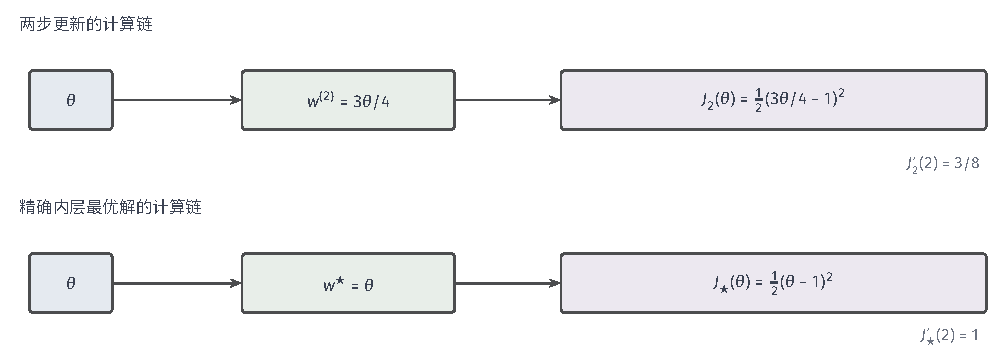
\includegraphics[width=168.998mm]{figures/01-mathematical-preliminaries-upper/01-mathematical-language-combinatorics-analysis-optimization/tikz/opt-bilevel-target-chains/figure.pdf}
  \caption{同一二次内层目标的两条计算链。固定$w^{(0)}=0$、步长$1/2$，两次更新产生$w^{(2)}=3\theta/4$；精确最优解则为$w^\star=\theta$。外层都读取$(w-1)^2/2$，但两个复合目标不同，故在$\theta=2$处分别得到导数$3/8$与$1$。有限步算法的求导与精确解分支的求导各自对应自己的目标。}
  \label{fig:opt-bilevel-target-chains}
\end{figure*}



隐式求导跟踪的是一个选定的非退化局部最小点分支，不自动证明该分支实现全局最小值。
只有当这个分支也是全局最小点并符合前述选择规则时，它才与
$\bm{w}^{\star}(\bm{\theta})$及$J$对应。为区分两者，记局部分支及其外层目标为
$\widehat{\bm{w}}(\bm{\theta})$和
$\widehat{J}(\bm{\theta})
=L_{\mathrm{out}}(\widehat{\bm{w}}(\bm{\theta}),\bm{\theta})$。
若$L_{\mathrm{in}}$二阶连续可微，并且
\[
  \nabla_{\bm{w}}L_{\mathrm{in}}
  (\widehat{\bm{w}}(\bm{\theta}),\bm{\theta})=\bm{0},
\]
记在该分支上计算的二阶导数为
$\bm{H}_{w,w}=\nabla_{\bm{w},\bm{w}}^2L_{\mathrm{in}}$和
$\bm{H}_{w,\theta}=\nabla_{\bm{w},\bm{\theta}}^2L_{\mathrm{in}}$。
对驻点方程关于$\bm{\theta}$求导得到
\[
  \bm{H}_{w,w}\frac{d\widehat{\bm{w}}}{d\bm{\theta}}
  +\bm{H}_{w,\theta}=\bm{0}.
\]
当$\bm{H}_{w,w}$可逆时，第~\ref{chap:mathematical-analysis}章的隐函数定理给出局部可微分支；
固定参数时，这个驻点在附近是孤立的。对非退化局部最小点，
$\bm{H}_{w,w}\succ\bm{0}$保证这一可逆性。链式法则于是给出
\begin{equation}
  \nabla_{\bm{\theta}}\widehat{J}
  =
  \nabla_{\bm{\theta}}L_{\mathrm{out}}
  -\bm{H}_{w,\theta}^{\top}
  \bm{H}_{w,w}^{-\top}
  \nabla_{\bm{w}}L_{\mathrm{out}}.
  \label{eq:opt-implicit-hypergradient}
\end{equation}
式~\eqref{eq:opt-implicit-hypergradient}是\term{隐式超梯度}
（implicit hypergradient）。实际计算通常解线性方程
$\bm{H}_{w,w}^{\top}\bm{v}=\nabla_{\bm{w}}L_{\mathrm{out}}$，无须显式求逆。

用二次内层目标可以核对公式。设$\bm H\in\mathbb R^{d\times d}$对称正定，$\bm B\in\mathbb R^{d\times p}$、$\bm C\in\mathbb R^{m\times d}$、$\bm d\in\mathbb R^m$，
\[
  L_{\mathrm{in}}(\bm{w},\bm{\theta})
  =\frac12(\bm{w}-\bm{B}\bm{\theta})^{\top}
  \bm{H}(\bm{w}-\bm{B}\bm{\theta}),\qquad
  L_{\mathrm{out}}(\bm{w})
  =\frac12\lVert\bm{C}\bm{w}-\bm{d}\rVert_2^2.
\]
这里内层最小点唯一，因此局部分支与全局选择一致：
$\widehat{\bm{w}}=\bm{w}^{\star}=\bm{B}\bm{\theta}$且
$\widehat{J}=J$。直接消元给出
\[
  \nabla_{\bm{\theta}}J
  =\bm{B}^{\top}\bm{C}^{\top}
  (\bm{C}\bm{B}\bm{\theta}-\bm{d}).
\]
隐式公式中$\bm{H}_{w,w}=\bm{H}$、
$\bm{H}_{w,\theta}=-\bm{H}\bm{B}$，代入后得到同一结果。计算时若线性方程残差为
$\bm r=\bm H^\top\widetilde{\bm v}-\nabla_{\bm w}L_{\mathrm{out}}$，
解误差为$\widetilde{\bm v}-\bm v=\bm{H}^{-\top}\bm{r}$；小特征值会放大该误差。因而内层驻点残差、
线性求解残差和曲率病态是三种不同的误差来源。

若内层只近似收敛，驻点残差会进入超梯度误差；若Hessian矩阵奇异，解映射可能不唯一或不可微；
若内层非凸，所选局部分支还依赖初始化与算法路径，并且可能不是全局最小点。后一种情况下，
式~\eqref{eq:opt-implicit-hypergradient}给出的是$\widehat{J}$的梯度，而不是前述全局
双层目标$J$的梯度。展开深度、线性方程精度、内层计算预算与解选择规则因此都是问题定义的
一部分，而不只是实现细节。

误差可在局部强凸条件下定量分开。固定$\bm\theta$，设近似点$\widetilde{\bm w}$
与选定分支$\widehat{\bm w}$之间的凸邻域满足
$\nabla_{\bm w,\bm w}^2L_{\mathrm{in}}\succeq\mu\bm I$，$\mu>0$。
内层残差$\bm r_{\mathrm{in}}=\nabla_{\bm w}L_{\mathrm{in}}(\widetilde{\bm w},\bm\theta)$满足
\[
 \|\widetilde{\bm w}-\widehat{\bm w}\|_2
 \leq\frac{\|\bm r_{\mathrm{in}}\|_2}{\mu},
\]
因为梯度沿线段积分后，与位移的内积至少为$\mu$倍距离平方。
在近似点计算内层Hessian$\widetilde{\bm H}$、混合导数
$\widetilde{\bm B}=\nabla_{\bm w,\bm\theta}^2L_{\mathrm{in}}(\widetilde{\bm w},\bm\theta)$
及外层梯度，再近似求解伴随方程，
令$\bm r_{\mathrm{lin}}=\widetilde{\bm H}^{\top}\widetilde{\bm v}
-\nabla_{\bm w}L_{\mathrm{out}}(\widetilde{\bm w},\bm\theta)$。
线性求解单独贡献的超梯度误差至多为
$\|\widetilde{\bm B}\|_2\|\bm r_{\mathrm{lin}}\|_2/\mu$。
若这些一、二阶导数在该邻域有界且Lipschitz，精确线性求解所定义的超梯度表达式
作为$\bm w$的函数有某个有限Lipschitz常数$C$。记由近似点与近似伴随解算出的
超梯度为$\widetilde{\nabla_{\bm\theta}\widehat J}$，则总误差满足
\begin{equation}
 \|\widetilde{\nabla_{\bm\theta}\widehat J}-\nabla_{\bm\theta}\widehat J\|_2
 \leq\frac C\mu\|\bm r_{\mathrm{in}}\|_2
 +\frac{\|\widetilde{\bm B}\|_2}{\mu}\|\bm r_{\mathrm{lin}}\|_2.
 \label{eq:opt-hypergradient-two-residuals}
\end{equation}
右侧第一项来自内层点不够准确，第二项来自同一点上的线性系统未解准。
只压低其中一项不足以控制总误差，小$\mu$也会同时放大二者。
取得外层方向后，可再对选定的外层目标执行梯度或投影更新；
只有所求超梯度对应的目标和误差范围明确，才能复用前面带误差更新的分析。

\section{本章小结}
\label{sec:opt-summary}

最优化需要分别回答四个问题：候选解是否存在，某个点为何最优，算法怎样到达它，以及误差
按什么尺度收敛。连续性配合紧致性保证存在；在闭域上，下半连续性与强制性也能通过紧
下水平集保证存在。凸性把局部条件提升为全局条件，强凸、光滑性与PL条件则分别控制参数
距离、单步上界和目标误差。它们不能只用“曲率好”一语合并。

共同二次目标$(w_1^2+16w_2^2)/2$展示了这些条件怎样进入计算：
统一梯度步受曲率$16$限制，动量改变历史响应，预条件调整两个方向的尺度，
牛顿法则直接解曲率方程。它们对同一个无约束答案付出不同的信息与计算成本。
加上$\ell_1$项后，软阈值使尖点可精确处理；加上$w_1+w_2=1$后，
二次惩罚的有限参数解仍不满足等式，乘子平衡才给出约束解$(16/17,1/17)$。
因此比较方法要固定原任务、返回质量及成本口径，不能只看更新式是否更复杂或步数是否更少。

带资源约束后，KKT条件描述目标梯度与约束法向量的平衡，对偶变量提供界和敏感性解释。
Farkas证书与线性规划强对偶说明最优值相等需要证明，不能从凸性直接跳得。松弛、对偶界与
可行解共同形成最优性证书；乘子更新提供寻找下界的过程，原解恢复仍需单独保证可行性。
预算例中，对偶值持续改善时原始副本仍可能违规，这正是不能把求解过程与证书混为一谈的原因。

\begin{samepage}
计算预算不足时，可以组合代理、分块及近似更新，但必须分别记录误差来源及其累计方式。
目标下降中的平方误差和，与轨迹偏差中的一次范数和，控制不同对象；
副本一致、块最优和联合最优也需要不同条件。多个指标进一步要求约定权重或Pareto比较，
竞争要求核验最坏响应及鞍点间隙，嵌套要求区分有限步输出、局部驻点分支与理想全局内层解。
这些答案都可以“足够好”，但必须说明好在哪个尺度、满足哪些约束、花了多少计算。
随机逼近还需要条件期望、噪声与平均动力学工具，策略评价则会复用本章的对偶与鞍点语言。
第~\ref{chap:functional-analysis-and-approximation}章将把有限维参数推广到函数空间，
区分表示存在性、逼近误差与函数类复杂度。

\end{samepage}

